\documentclass[a4paper,twoside,UTF8]{ctexbook}


%%%%%%%%%%%%%%%%%%%%%%%%%%%%% 字 体 与 版 式 %%%%%%%%%%%%%%%%%%%%%%%%%%%%%%

\usepackage[charter]{mathdesign}
\setCJKmainfont{方正聚珍新仿简体}
\setCJKfamilyfont{hei}{FZYouHeiS}

\usepackage{geometry}
\geometry{
 a4paper,
 total={170mm,257mm},
 left=20mm,
 top=20mm,
 }
\usepackage{fancyhdr} 
\pagestyle{fancy}
\cfoot{\hei 学而思培优}
\fancyfoot[RO,LE]{\bfseries \thepage}

%%%%%%%%%%%%%%%%%%%%%%%%%%%%%%%%%%%%%%%%%%%%%%%%%%%%%%%%%%%%%%%%%%%%%%%%%%%


%%%%%%%%%%%%%%%%%%%%%%%%%%%%%    宏    包    %%%%%%%%%%%%%%%%%%%%%%%%%%%%%%

\usepackage{graphicx}
\usepackage[colorlinks=true, linkcolor=blue]{hyperref}
\usepackage[squaren]{SIunits}
\usepackage{caption}
\usepackage{CJKfntef}
\usepackage{wrapfig}
\usepackage{tagging}
\usepackage{float}
\usepackage{array}
\usepackage{xcolor}
\usepackage{mdframed}
\usepackage{lmodern}
\usepackage{upgreek}
\usepackage{amsbsy}
\usepackage{amsmath}
\usepackage{eucal}
\usepackage{enumerate}
\usepackage[T1]{fontenc}
\usepackage[utf8]{inputenc}

%%%%%%%%%%%%%%%%%%%%%%%%%%%%%%%%%%%%%%%%%%%%%%%%%%%%%%%%%%%%%%%%%%%%%%%%%%%


%%%%%%%%%%%%%%%%%%%%%%%%%%%%% 命 令 与 环 境 %%%%%%%%%%%%%%%%%%%%%%%%%%%%%%

\renewcommand{\emph}[1]{{\color{red} #1}}
\renewcommand{\arraystretch}{1.5}
\newcommand{\hei}{\CJKfamily{hei}}
\newcommand{\npg}[1]{\vspace{#1}\newpage}
\newcommand{\bs}[1]{\boldsymbol{#1}}
\newcommand{\sidenote}[1]{\marginpar{#1}}
\newcommand{\pow}[1]{\times 10^{#1}}
\newcommand{\dgr}{^\circ}
\newcommand{\cdgr}{^\circ \mathrm{C}}
\newcommand{\si}[1]{\mathrm{#1}}
\newcommand{\ud}{\textrm{d}}
\newcommand{\ue}{{\rm e}}
\newcommand{\ui}{{\rm i}}
\newcommand{\ke}{\frac{1}{4\pi\varepsilon_0}}
\newcommand{\kb}{\frac{\mu_0}{4\pi}}
\newcommand{\ca}{\raisebox{0.5mm}{------}\,}
\newcommand{\dbar}{\textrm{\dj}}
\newcommand{\intl}{\int\limits}
\newcommand{\ointl}{\oint\limits}

%%%%%%%%%%%%%%%%%%%%%%%%%%%%%%%%%%%%%%%%%%%%%%%%%%%%%%%%%%%%%%%%%%%%%%%%%%%%


%%%%%%%%%%%%%%%%%%%%%%%%%%%%%%     正    文    %%%%%%%%%%%%%%%%%%%%%%%%%%%%%

\title{\hei \Huge 高二物理竞赛 \\ 电磁学与近代物理}
\author{陈博}
\date{}


\begin{document}

\frontmatter
\maketitle
\usetag{teacher}

\mainmatter
\tableofcontents

%!TEX root = ../physical-olympics-2.tex
\chapter{静电学}


\section{电荷与电场}

\subsection{电磁相互作用与电荷}
物质若携带\emph{电荷}(charge),\,则可以发生\emph{电磁相互作用}(electromagnetic interaction).\,在经典情形下理解为电荷受到一个力.\,我们先研究\emph{静电学}(electrostatics),\,它要求受力物体与施力物体\footnote{实际上物理上不允许超距的施力物体,\,施力物体就是局域的电场.}都处于静止状态,\,或者认为一切电荷都处于静止状态.

电荷分正负,\,阴阳激荡.

作为协变电磁场理论的基本要求与实验规律,\,电荷是一个参考系不变的标量,\,微观地看电荷具有\emph{量子化}(quantized)的奇妙特性\footnote{与磁单极子的存在与量子化有关.}.\,质子的质量与电子的质量没有简单的整数比关系,\,但电荷量确实严格相反.\,如果设想两者电量有着微小差异,\,那么构成自然界的原子也就携带了一个能够传递远程相互作用的库仑力,\,从而导致自然界的不稳定\footnote{是的,\,这种思考方式就是\emph{人择原理}(antropic principle).}.\,而\emph{质子}(proton)的电量被定义为\emph{基本电荷}(elementary charge)\footnote{这个值是2018新国际标准单位制提出的规定值.}:
\[e=1.602176634\pow{-19} {\rm C}\]

实际上今天我们知道,\,电荷量的量子化单位实际上更小,\,至少是\(\dfrac{1}{3}e\),\,夸克的电量就是这个电量的一倍或两倍,\,可正可负.\,而\emph{电子}(electron)带一个单位的负电荷.\,当然,\,特殊场合还会有带一个单位正电荷的\emph{正电子}(positron)和一个单位负电荷的\emph{反质子}(anti-proton)甚至它们组成的反物质.\,\emph{中子}(proton)是不带电的.

\begin{wrapfigure}[16]{o}[-10pt]{7cm}
\centering
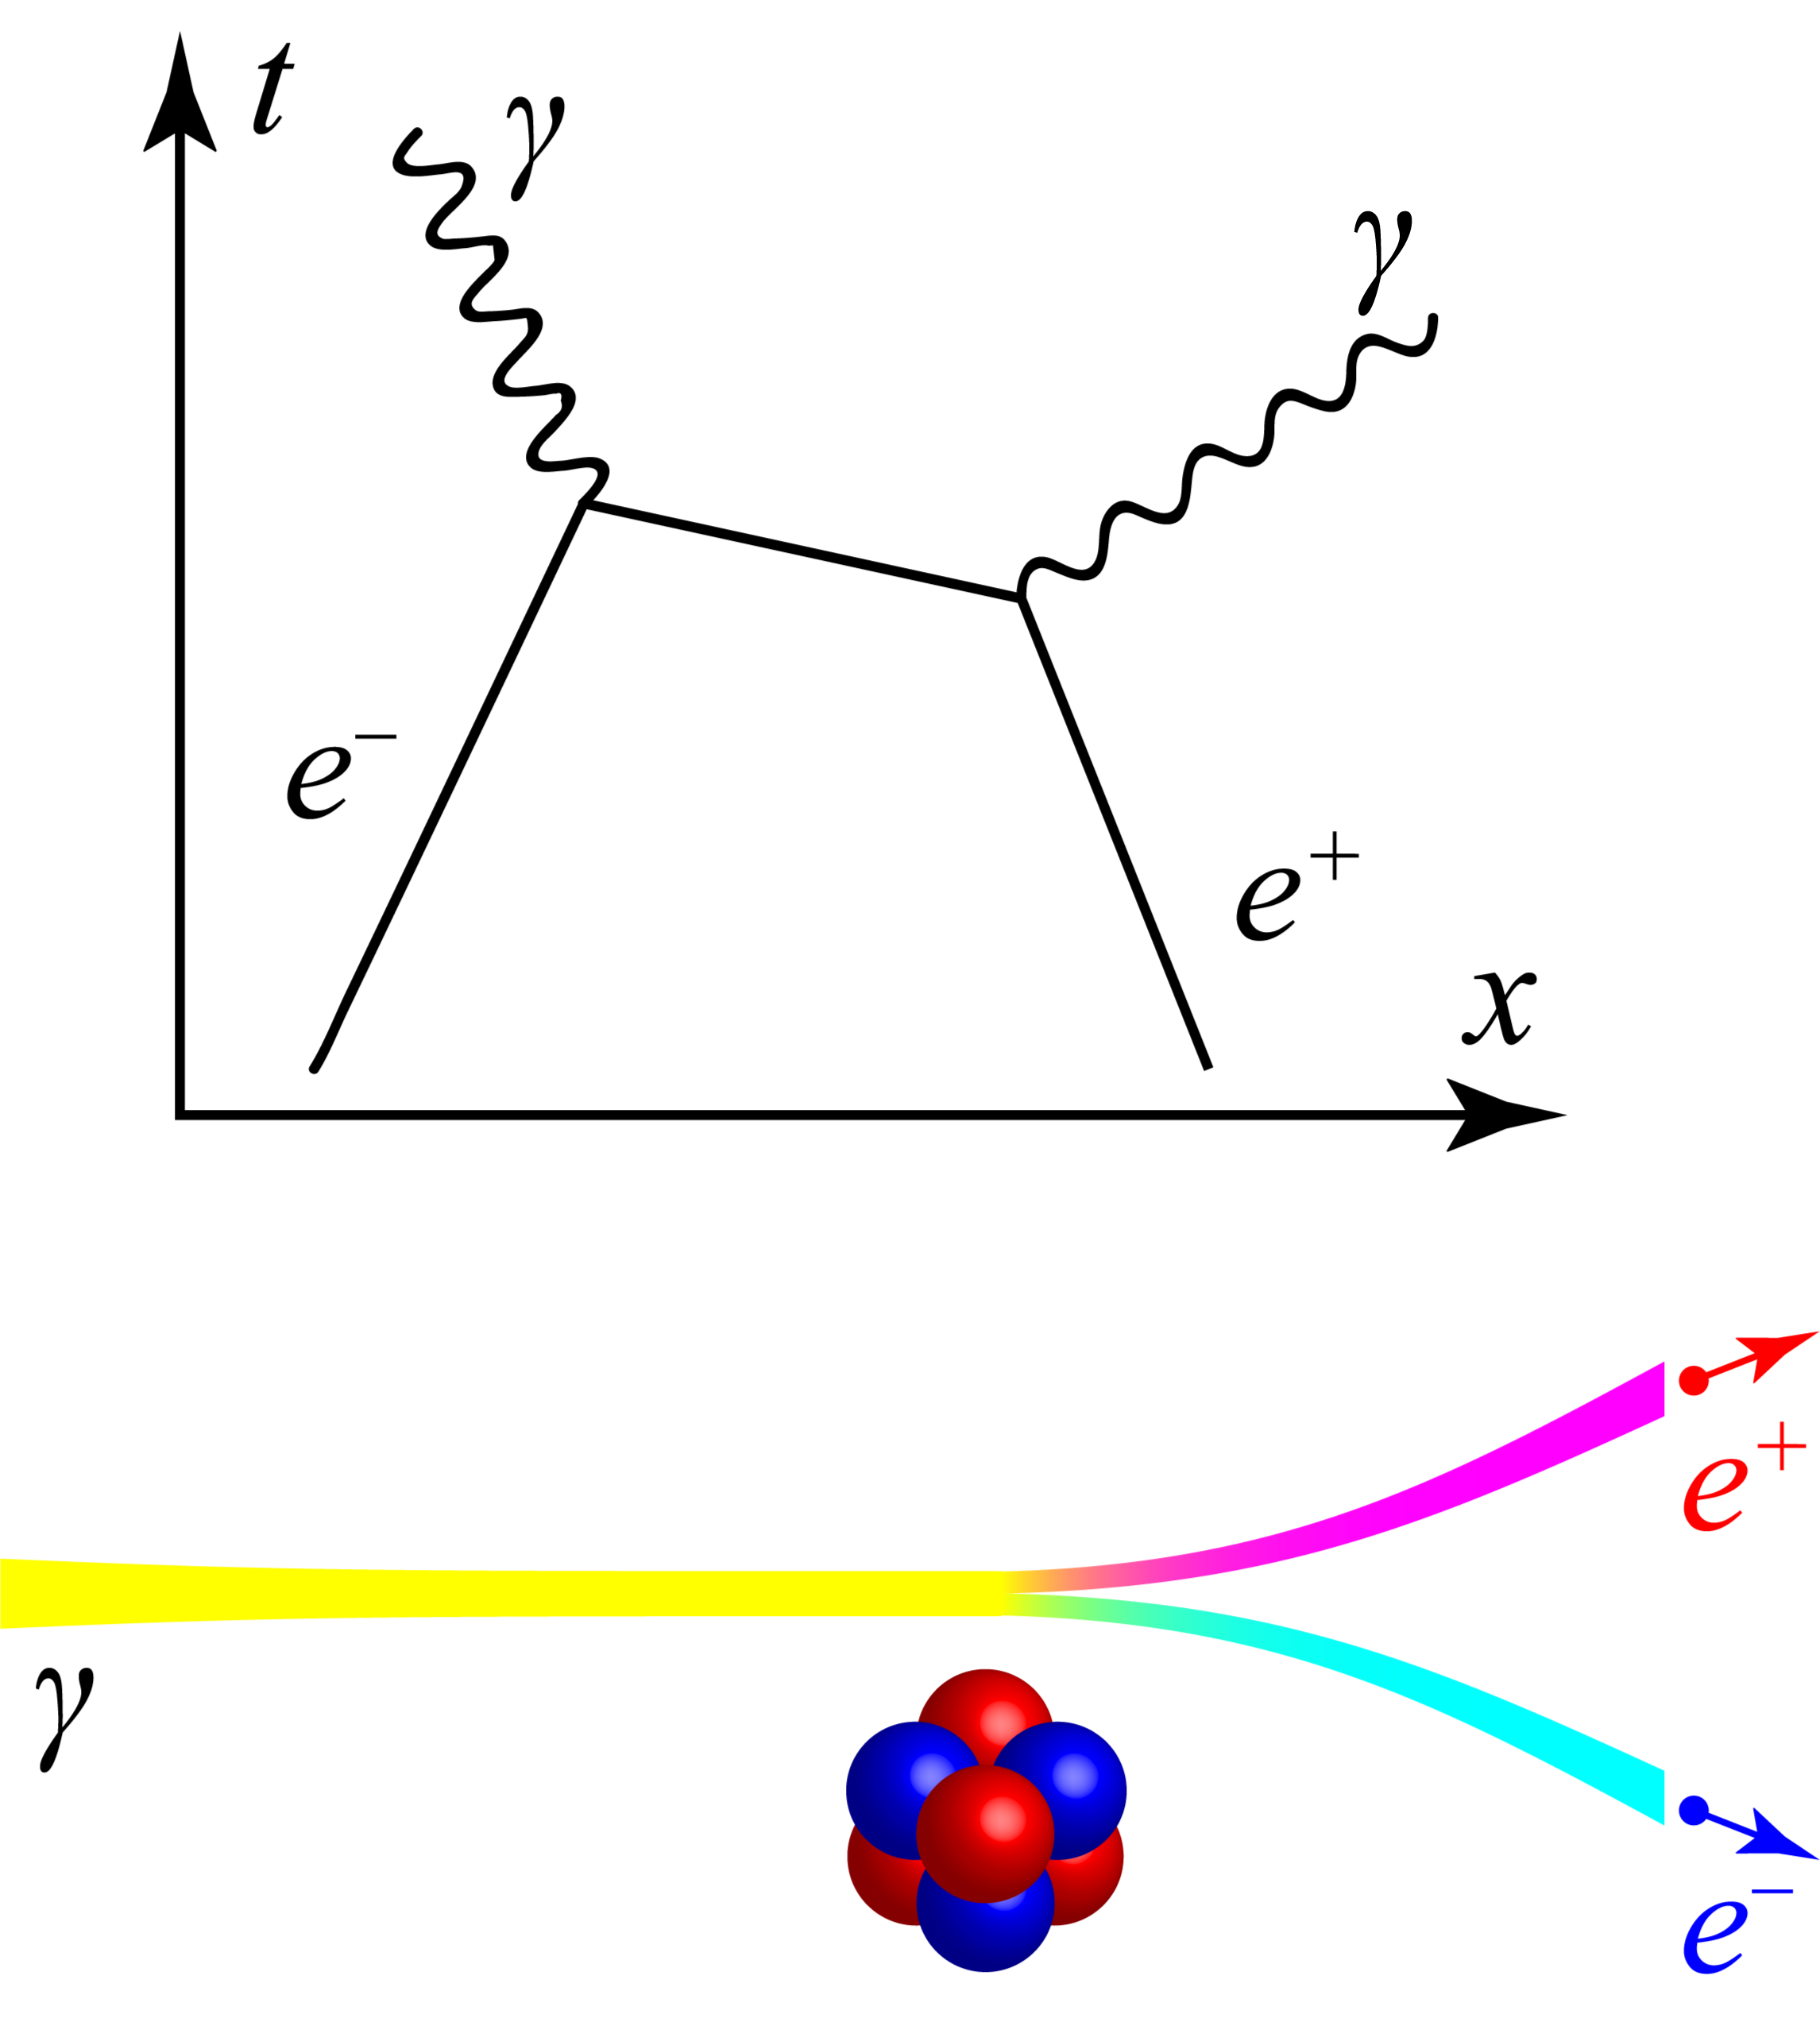
\includegraphics[width=7cm]{image/7-1-1.png}
\caption{电子对湮灭与产生}
\end{wrapfigure}
电荷如同静质量,\,是基本粒子的基本属性.\,它只能随着基本粒子运动,\,没有相互作用时不能被创造与消灭.\,在存在电磁相互作用时电荷可以被创造与消灭,\,典型的过程如电子与正电子\emph{湮灭}(annihilation)为两个光子或高能光子在原子核附近\emph{产生}(production)电子正电子对.\,这些过程电荷的代数和守恒,\,其实现要求反物质与相对论性运动的存在.\,在经典情形下有严格的\emph{电荷守恒定律}(charge conservation),\,电荷可以流动形成电流,\,但流动的过程中电荷的总量不能发生改变.\,我们总是计算一定体积内的电荷代数和:
\[\ud Q=\sum_i{n_i q_i}\ud V\]

其中\(n_i\)是第\(i\)种基本构成粒子的数密度,\,\(q_i\)是这种基本粒子的带电量.\,\(\ud V\)则为微元体积.\,而上式也被写为:
\[\ud Q=\rho \ud V\quad;\quad \rho=\sum_i{n_i q_i}=\sum_i \rho_i\]

\subsection{库仑定律}
\emph{库仑定律}(Coulumb's law)用于描述真空中的两个孤立静止点电荷之间的相互作用力:
\[\bs{F}_{12}=\ke\frac{q_1q_2}{r^2}\bs{e}_{12}\]

其中系数\(k_e=\dfrac{1}{4\pi \varepsilon_0}\approx 8.99\pow{9}{\rm N\cdot m^{-2} \cdot C^{-2}}\)为库仑常数.

\begin{wrapfigure}[11]{o}[-10pt]{7cm}
\centering
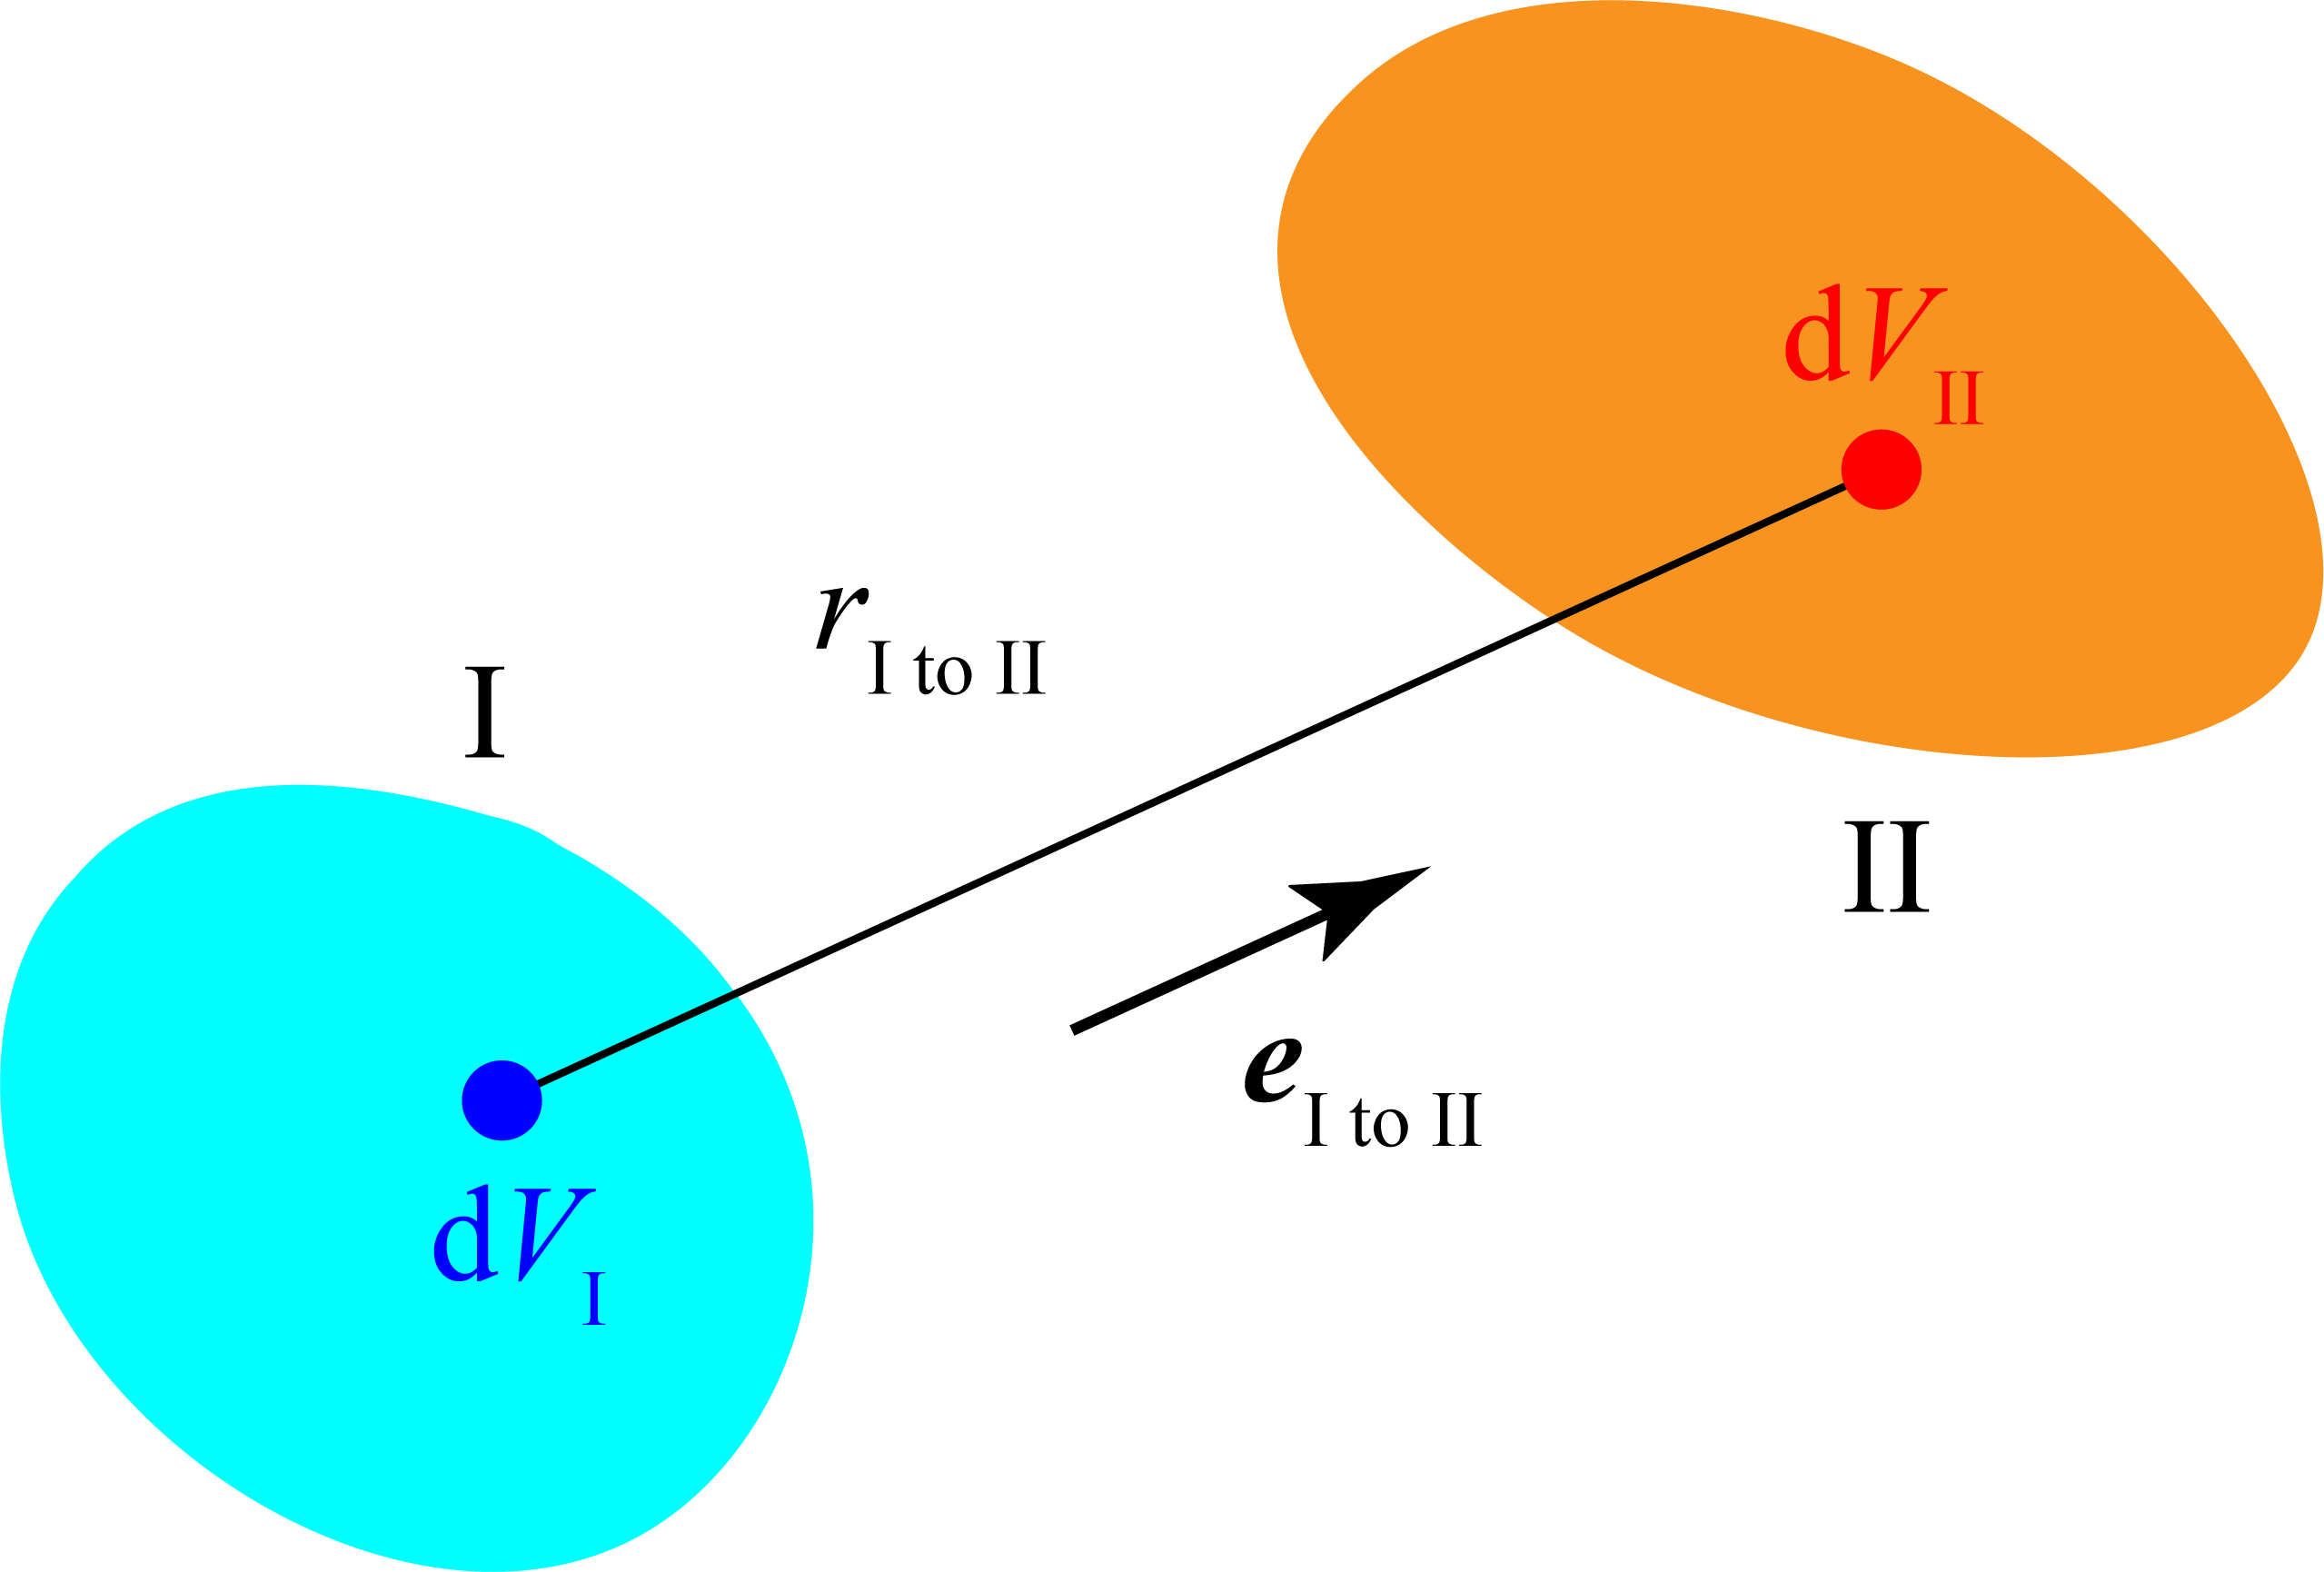
\includegraphics[width=7cm]{image/7-1-2.png}
\caption{电荷体系间的相互作用力}
\end{wrapfigure}
库仑定律是整个电磁学最基本的公理.\,其他所有规律或多或少都可以理解为库仑定律与自洽的物理概念体系的推论.\,库仑定律的特征是:

1.{\hei 平方反比(inverse-square law)}:\,与万有引力相似,\,与强相互作用与弱相互作用不同,\,荷之间的相互作用力遵从平方反比律.\,这一点使得此相互作用成为\emph{长程}(long range)相互作用,\,长至\(10^7{\rm m}\),\,短至\(10^{-17}{\rm m}\),\,库仑定律被证明是有效的.\,更短的距离下则由于量子场论的原因而使得基本电荷量的值上升,\,但基本的规律仍然不变.

2.{\hei 叠加原理(superposition principle)}:\,力与电荷成正比,\,而电荷在概念上可以作为标量线性叠加,\,说明了力的叠加本性.\,一个复杂电荷系统(包括构成介质的电荷)可以用连续的电荷密度描述:
\[\ud Q=\rho \ud V\]
	
那么两部分电荷之间的相互作用力为:
\[\bs{F}_{\rm I\,to\,II}=\ke\int\limits_{V_{\rm II}}\rho(\bs{r}_{\rm II})\int\limits_{V_{\rm I}}\frac{\rho(\bs{r}_{\rm I})}{r_{\rm I\,to\,II}^2}\bs{e}_{\rm I\,to\,II}\ud V_{\rm I}\ud V_{\rm II}\]

相互作用力在定义上就是成对存在的,\,所以两部分电荷体系间的相互作用力满足牛顿第三定律:\,大小相等,\,方向相反,\,对整个体系产生的力矩的贡献为零.

\vspace{1cm}
\subsection{电场}
现代物理认为,\,狭义相对论下的时空观是正确的.\,一个重要的推论就是\emph{局域性原理}(principle of locality):\,物体仅仅被此时此刻周围的物质所影响.\,所有相互作用必须被理解为\emph{近距作用}(action upon contact)而不能是\emph{超距作用}(action at a distance).\,这是为了能与更本质的\emph{因果律}(principle of causality)相适应.\,如果物体这一时刻的状态及其改变取决于同一时刻的空间上相隔一定距离的另外一个点(类空间隔).\,那么就可以另一个点的事件称作因,\,而物体的状态与状态改变称作果.\,但类空间隔在洛伦兹变换下具有可逆性.\,也就是原则上可以在果的时空点也可以制造事件去对因的点产生影响.\,从而造成逻辑上的紊乱.\,所以我们必须规定这两个时空点间不存在因果关系,\,互相独立没有影响.

局域性原理的直接结论便是,\,在引力与电磁相互作用时,\,作为物质的\emph{场}(field)的概念的引入.\,场本是数学概念.\,在一个三维的欧几里得空间\(\mathbb{R}^3\)中,\,如果每一个点都定义了一个数(标量),\,代表某种物理量,\,物理现象可以在不同参考系,\,惯性系中观察,\,所对应的时空点的位置坐标可能发生改变,\,但特定的时空点的概念,\,和与之相结合的物理现象与描述它的这个数,\,不应该发生改变,\,称为\emph{标量}(scalar):
\[\mathfrak{f}:\quad \bs{r}\mapsto f(\bs{r})\]
\npg{0cm}
\begin{wrapfigure}[15]{o}[0pt]{6cm}
\centering
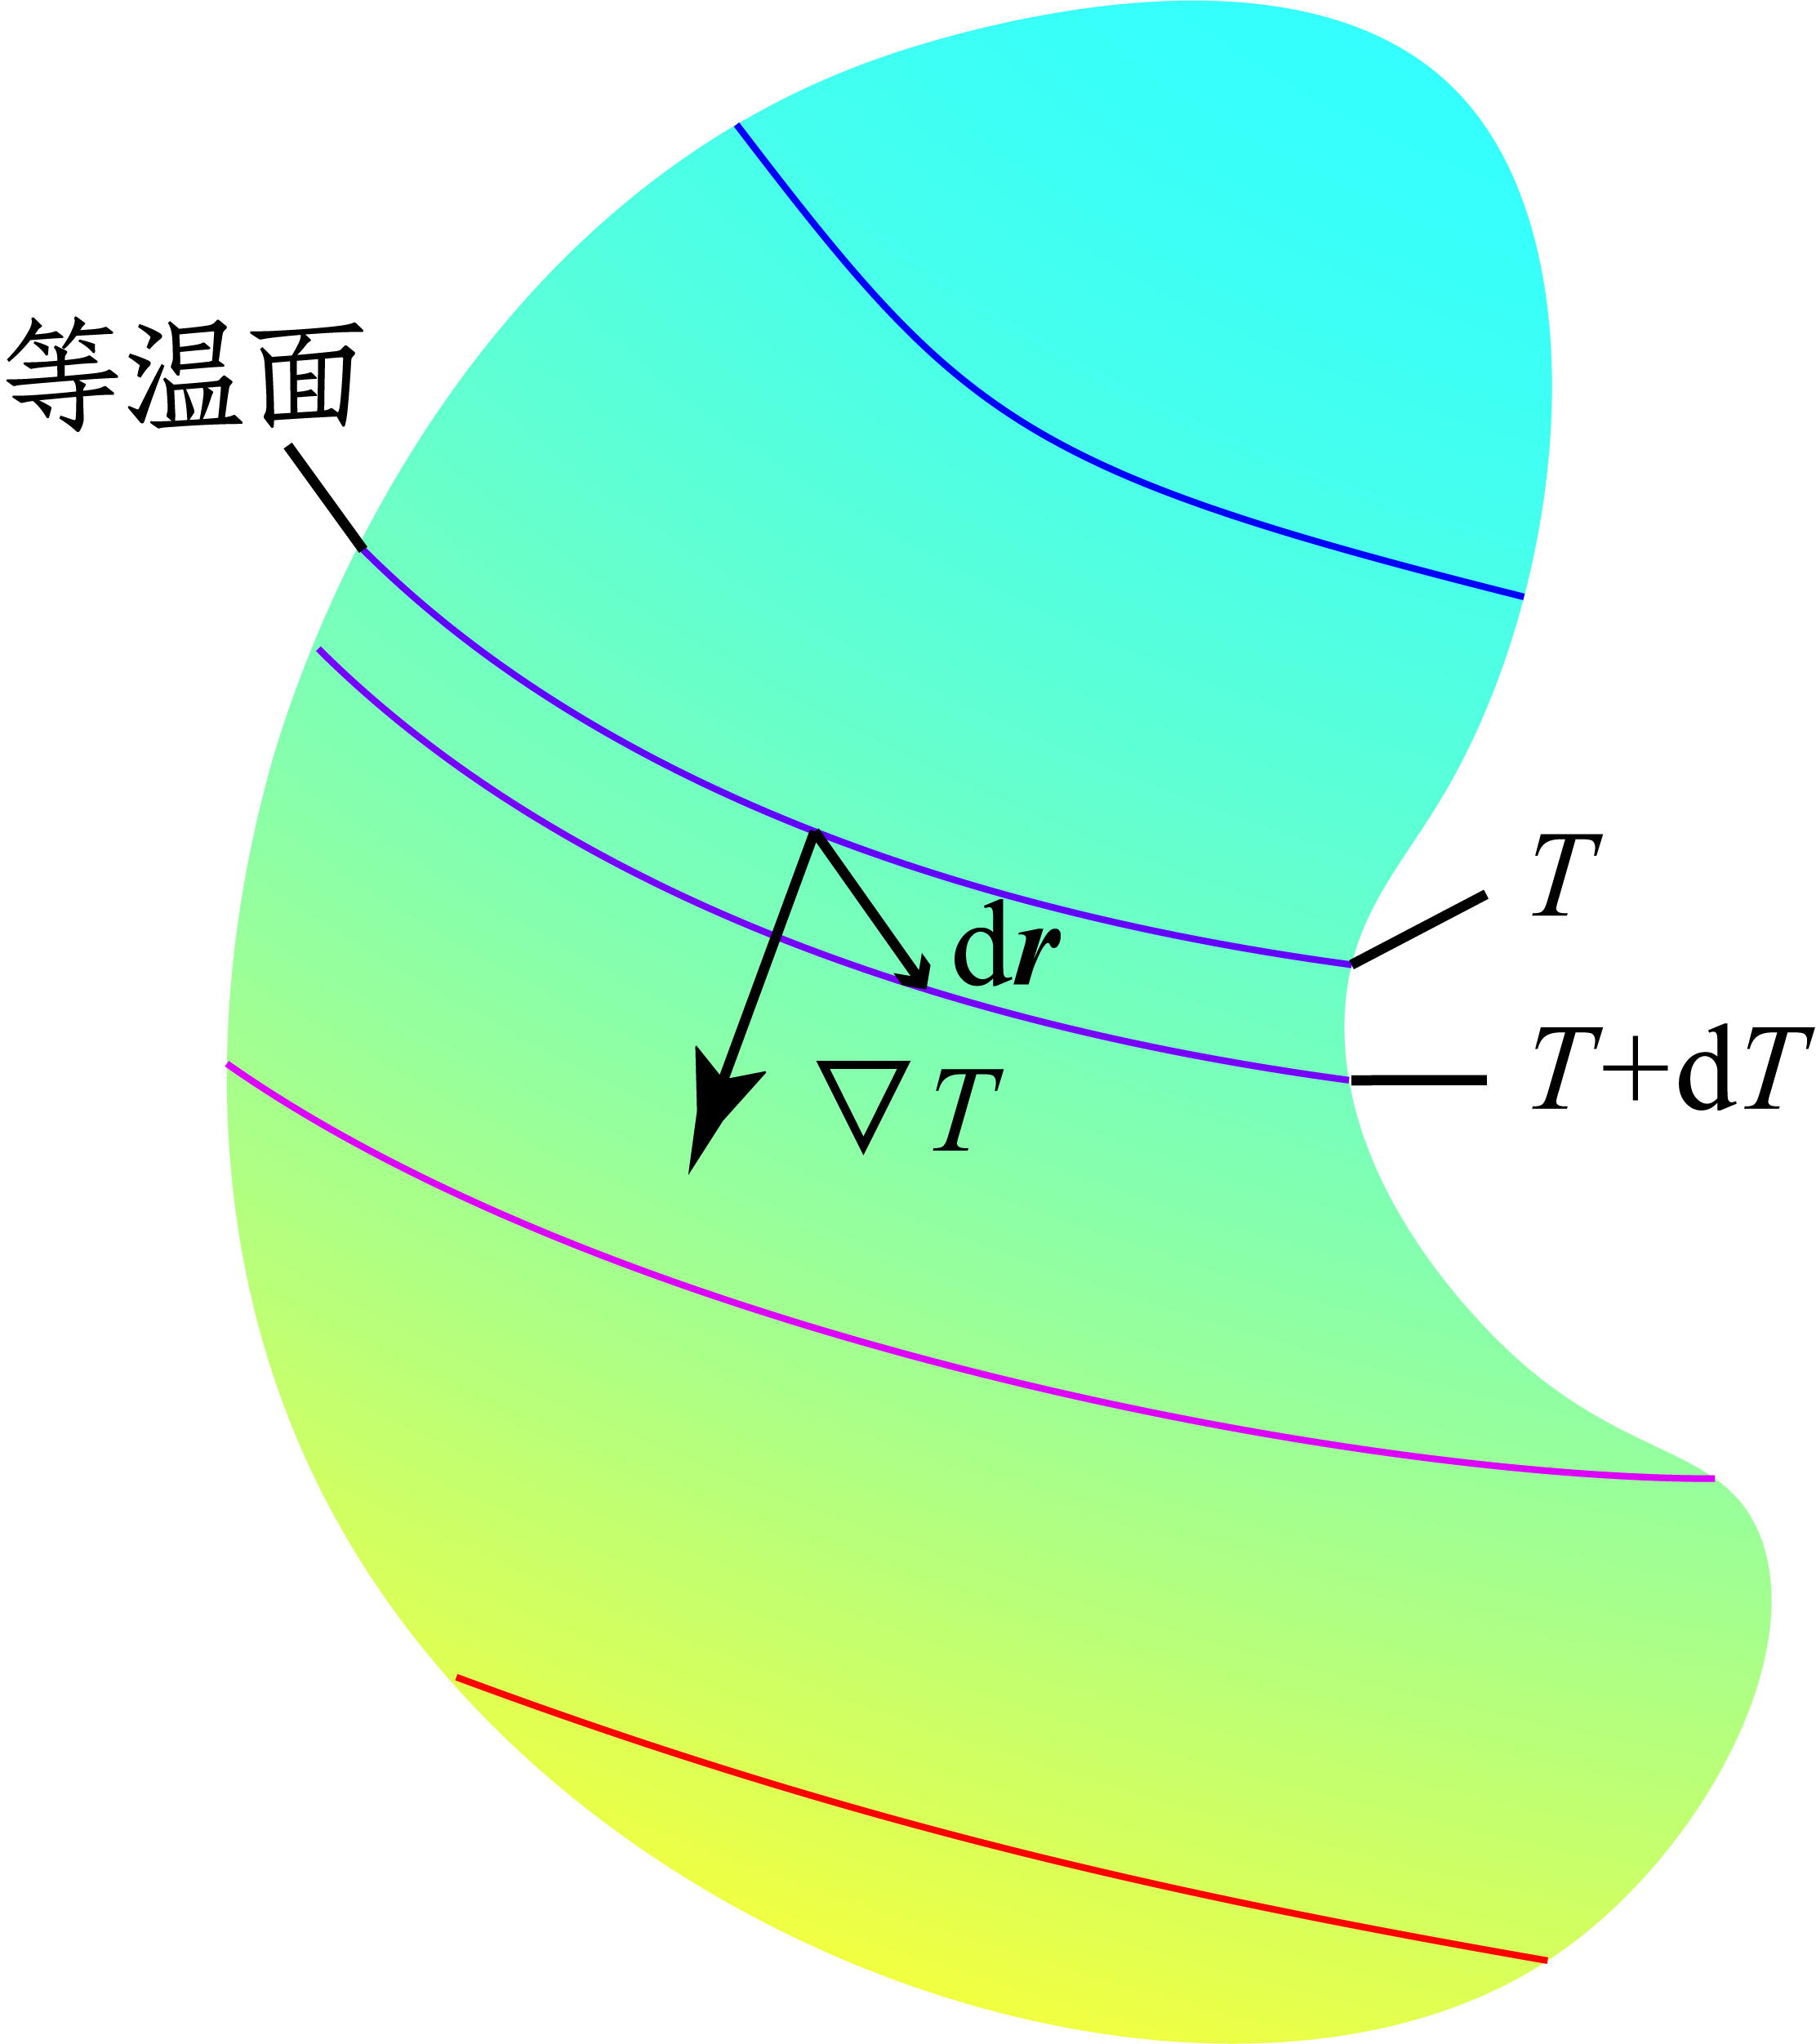
\includegraphics[width=6cm]{image/7-1-3.png}
\caption{温度场的梯度}
\end{wrapfigure}
如,\,压强场,\,温度场,\,波动的相位场,\,都是典型的标量场的例子.\,数学上定义了标量场的\emph{梯度}(gradient)来描述在一点极其附近的标量场的行为,\,它是一个矢量,\,方向是使得标量上升最快的欧几里得空间中的方向,\,大小是沿这个方向的标量变化的方向导数.\,数学上可以证明:
\[\nabla f=\frac{\partial f}{\partial x}\bs{e}_x+\frac{\partial f}{\partial y}\bs{e}_y+\frac{\partial f}{\partial z}\bs{e}_z\]

物理量在某点\(\bs{r}\)的局部,\,偏离一个\(\ud \bs{r}\)后值变为:
\[f(\bs{r}+\ud\bs{r})=f(\bs{r})+\nabla f\cdot\ud \bs{r}\]

这就是微元形式的\emph{牛顿-莱布尼茨定理}(Newton-Leibniz theorem).\,而标量场的梯度往往也具有重要的含义.\,压强场的梯度决定浮力的方向与大小(反向),\,温度场的梯度决定热传导的方向与强弱(也是反向),\,波动的相位场的梯度则决定波的传播方向与波长(波矢).

而在三维的欧几里得空间中在每一个空间点也可以引入一个\emph{矢量}(vector),\,它不占三维空间的有限体积\footnote{即,\,不同于位移矢量那样必须与三维空间中的不同点同时建立联系}而是定义在一个点上,\,可以认为是这个点上扩展出了一个新的与原三维空间坐标平行的\(\bs{e}_x-\bs{e}_y-\bs{e}_z\)坐标系.\,而这一点定义的矢量就位于这个``浓缩在一点''的坐标系中\footnote{数学术语把空间叫做\emph{微分流形}(differentiable manifold),\,而局部的矢量位于的空间叫做\emph{纤维}(fiber)或\emph{切空间}(tagent space),\,每一点都有一个这样的空间,\,合称\emph{纤维丛}(fiber bundle).}:
\[\mathfrak{F}:\quad \bs{r}\mapsto\bs{F}(\bs{r})\]

显然,\,标量场的梯度恰是一个矢量场.\,矢量不能简单理解为三个标量场的合成.\,因为在空间旋转(或时空的惯性系变化)下,\,标量应该是不变的,\,而矢量将发生与坐标系相似的旋转,\,从而三个分量之间相互转化,\,只有矢量的模长是不变的.\,另一种典型的矢量场是流体的流速场\(\bs{v}\),\,或者更普遍的,\,某种物理属性的流密度场\(\bs{j}\),\,前者定义为单位时间通过单位面积的体积,\,后者则推广为单位时间通过单位面积的某物理量\(Q\):
\[\ud Q=\bs{j}\cdot\ud A\ud t\]

在一点附近的矢量场的行为则比标量场复杂很多:
\[\bs{F}(\bs{r}+\ud\bs{r})=\bs{F}(\bs{r})+\ud \bs{r}\cdot\nabla \bs{F}\]

此处\(\nabla=\bs{e}_x\dfrac{\partial}{\partial x}+\bs{e}_y\dfrac{\partial}{\partial y}+\bs{e}_z\dfrac{\partial}{\partial z}\)可以形式地视为矢量微分算符,\,它写在上一式的后一项中实际上是在表示:
\begin{align*}
\ud \bs{F} 	&=\ud F_x \bs{e}_x+\ud F_y \bs{e}_y+\ud F_x \bs{e}_z \\
			&=(\frac{\partial F_x}{\partial x}\ud x+\frac{\partial F_x}{\partial y}\ud y+\frac{\partial F_x}{\partial z}\ud z)\bs{e}_x\\
			&\phantom{=}+(\frac{\partial F_y}{\partial x}\ud x+\frac{\partial F_y}{\partial y}\ud y+\frac{\partial F_y}{\partial z}\ud z)\bs{e}_y\\
			&\phantom{=}+(\frac{\partial F_z}{\partial x}\ud x+\frac{\partial F_z}{\partial y}\ud y+\frac{\partial F_z}{\partial z}\ud z)\bs{e}_z\\
			&=(\ud x\frac{\partial}{\partial x}+\ud y\frac{\partial}{\partial y}+\ud z\frac{\partial}{\partial z})(F_x\bs{e}_x+F_y\bs{e}_y+F_z\bs{e}_z)\\
			&=\ud \bs{r}\cdot\nabla \bs{F}
\end{align*}

而也可以把\(\nabla \bs{F}\)认为能完整描述这个矢量在该点处的一阶变化行为,\,也称为矢量的梯度,\,但它实际上由九个分量组成,\,分别描述三个分量在三个方向的变化率,\,一般写在一张数表中,\,也就是矩阵\footnote{实际上,\,形成了一个\emph{张量场}(tensor filed).\,张量将不在本部分教材的讨论范围内.}:
\[\nabla \bs{F}=\begin{bmatrix}
\dfrac{\partial F_x}{\partial x}&\dfrac{\partial F_y}{\partial x}&\dfrac{\partial F_z}{\partial x}\\[3pt]
\dfrac{\partial F_x}{\partial y}&\dfrac{\partial F_y}{\partial y}&\dfrac{\partial F_z}{\partial y}\\[3pt]
\dfrac{\partial F_x}{\partial z}&\dfrac{\partial F_y}{\partial z}&\dfrac{\partial F_z}{\partial z}
\end{bmatrix}\]

显然用这样的一个矩阵去描述矢量场在一点处的行为是代数的,\,抽象地,\,不几何直观的.\,所以我们引入两个物理上会更实用的概念.

\begin{wrapfigure}[16]{o}[0pt]{7cm}
\centering
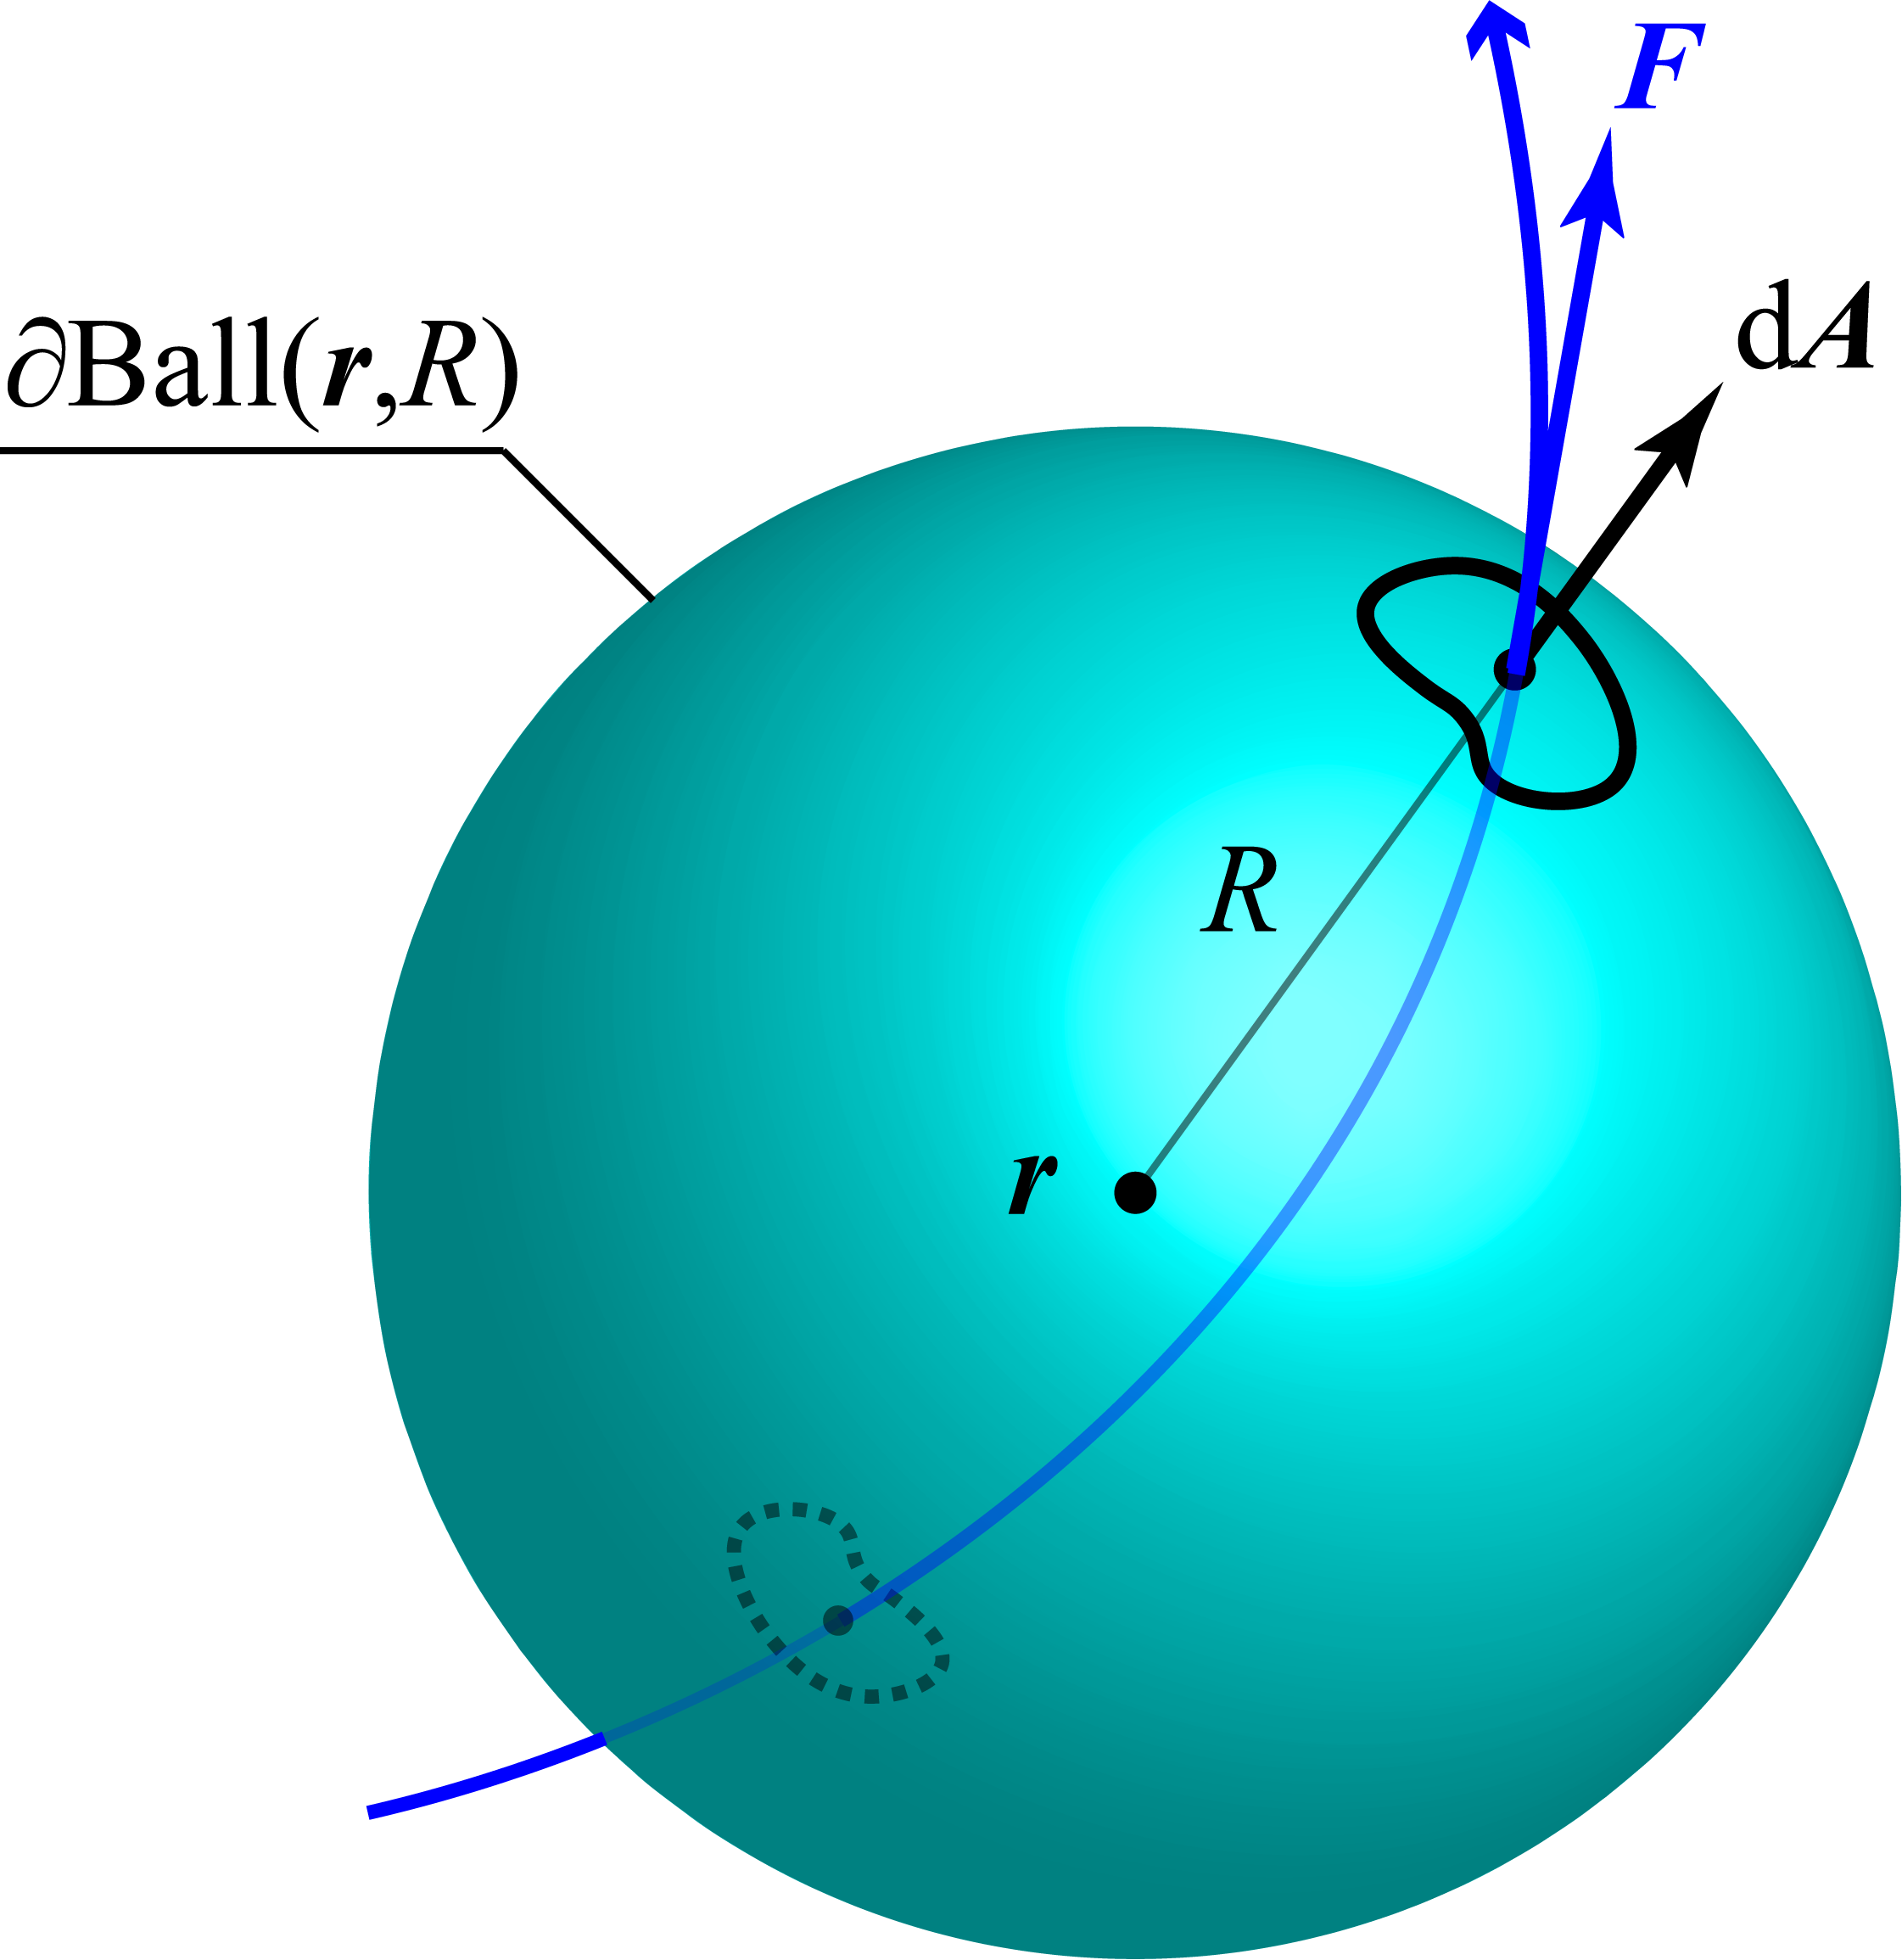
\includegraphics[width=7cm]{image/7-1-4.png}
\caption{矢量场的散度}
\end{wrapfigure}
一是矢量场的\emph{散度}(divergence),\,它是一个标量,\,定义为矢量场的源强度:
\[\nabla\cdot \bs{F}=\lim_{R\to 0}\left.\left(\oint_{\partial {\rm Ball}(\bs{r},R)}\bs{F}\cdot \ud\bs{A}\right)\right/(\frac{4}{3}\pi R^3)\]

其中\({\rm Ball}(\bs{r},R)\)表示以待研究的点为球心的,\,半径为\(R\)的球形体,\,而\(\partial {\rm Ball}\)表示它的表面.\,积分号\(\oint\)用来代表此场合下用来积分的区域是一个闭合的区域\footnote{数学上称为\emph{又闭又开}(clopen)的集合,\,表示它没有边界.}.\,积分的量称为\emph{通量}(flux),\,即矢量场与面积的电场,\,速度场情况下即单位时间通过面\(\ud \bs{A}\)的体积.\,现在对闭合的面进行积分,\,再除以面包含的体积,\,代表的是该点单位体积内产生这个矢量场的场线的源的多少,\,即源强度.\,数学上可以证明,\,它与体积以怎样的取法趋于零无关,\,如果取成与坐标系平行的长方体的形状,\,能够在坐标系下计算出它的值为:
\[\nabla\cdot\bs{F}=\frac{\partial F_x}{\partial x}+\frac{\partial F_y}{\partial y}+\frac{\partial F_z}{\partial z}\]

\begin{wrapfigure}[15]{o}[0pt]{7cm}
\centering
\vspace{0.5cm}
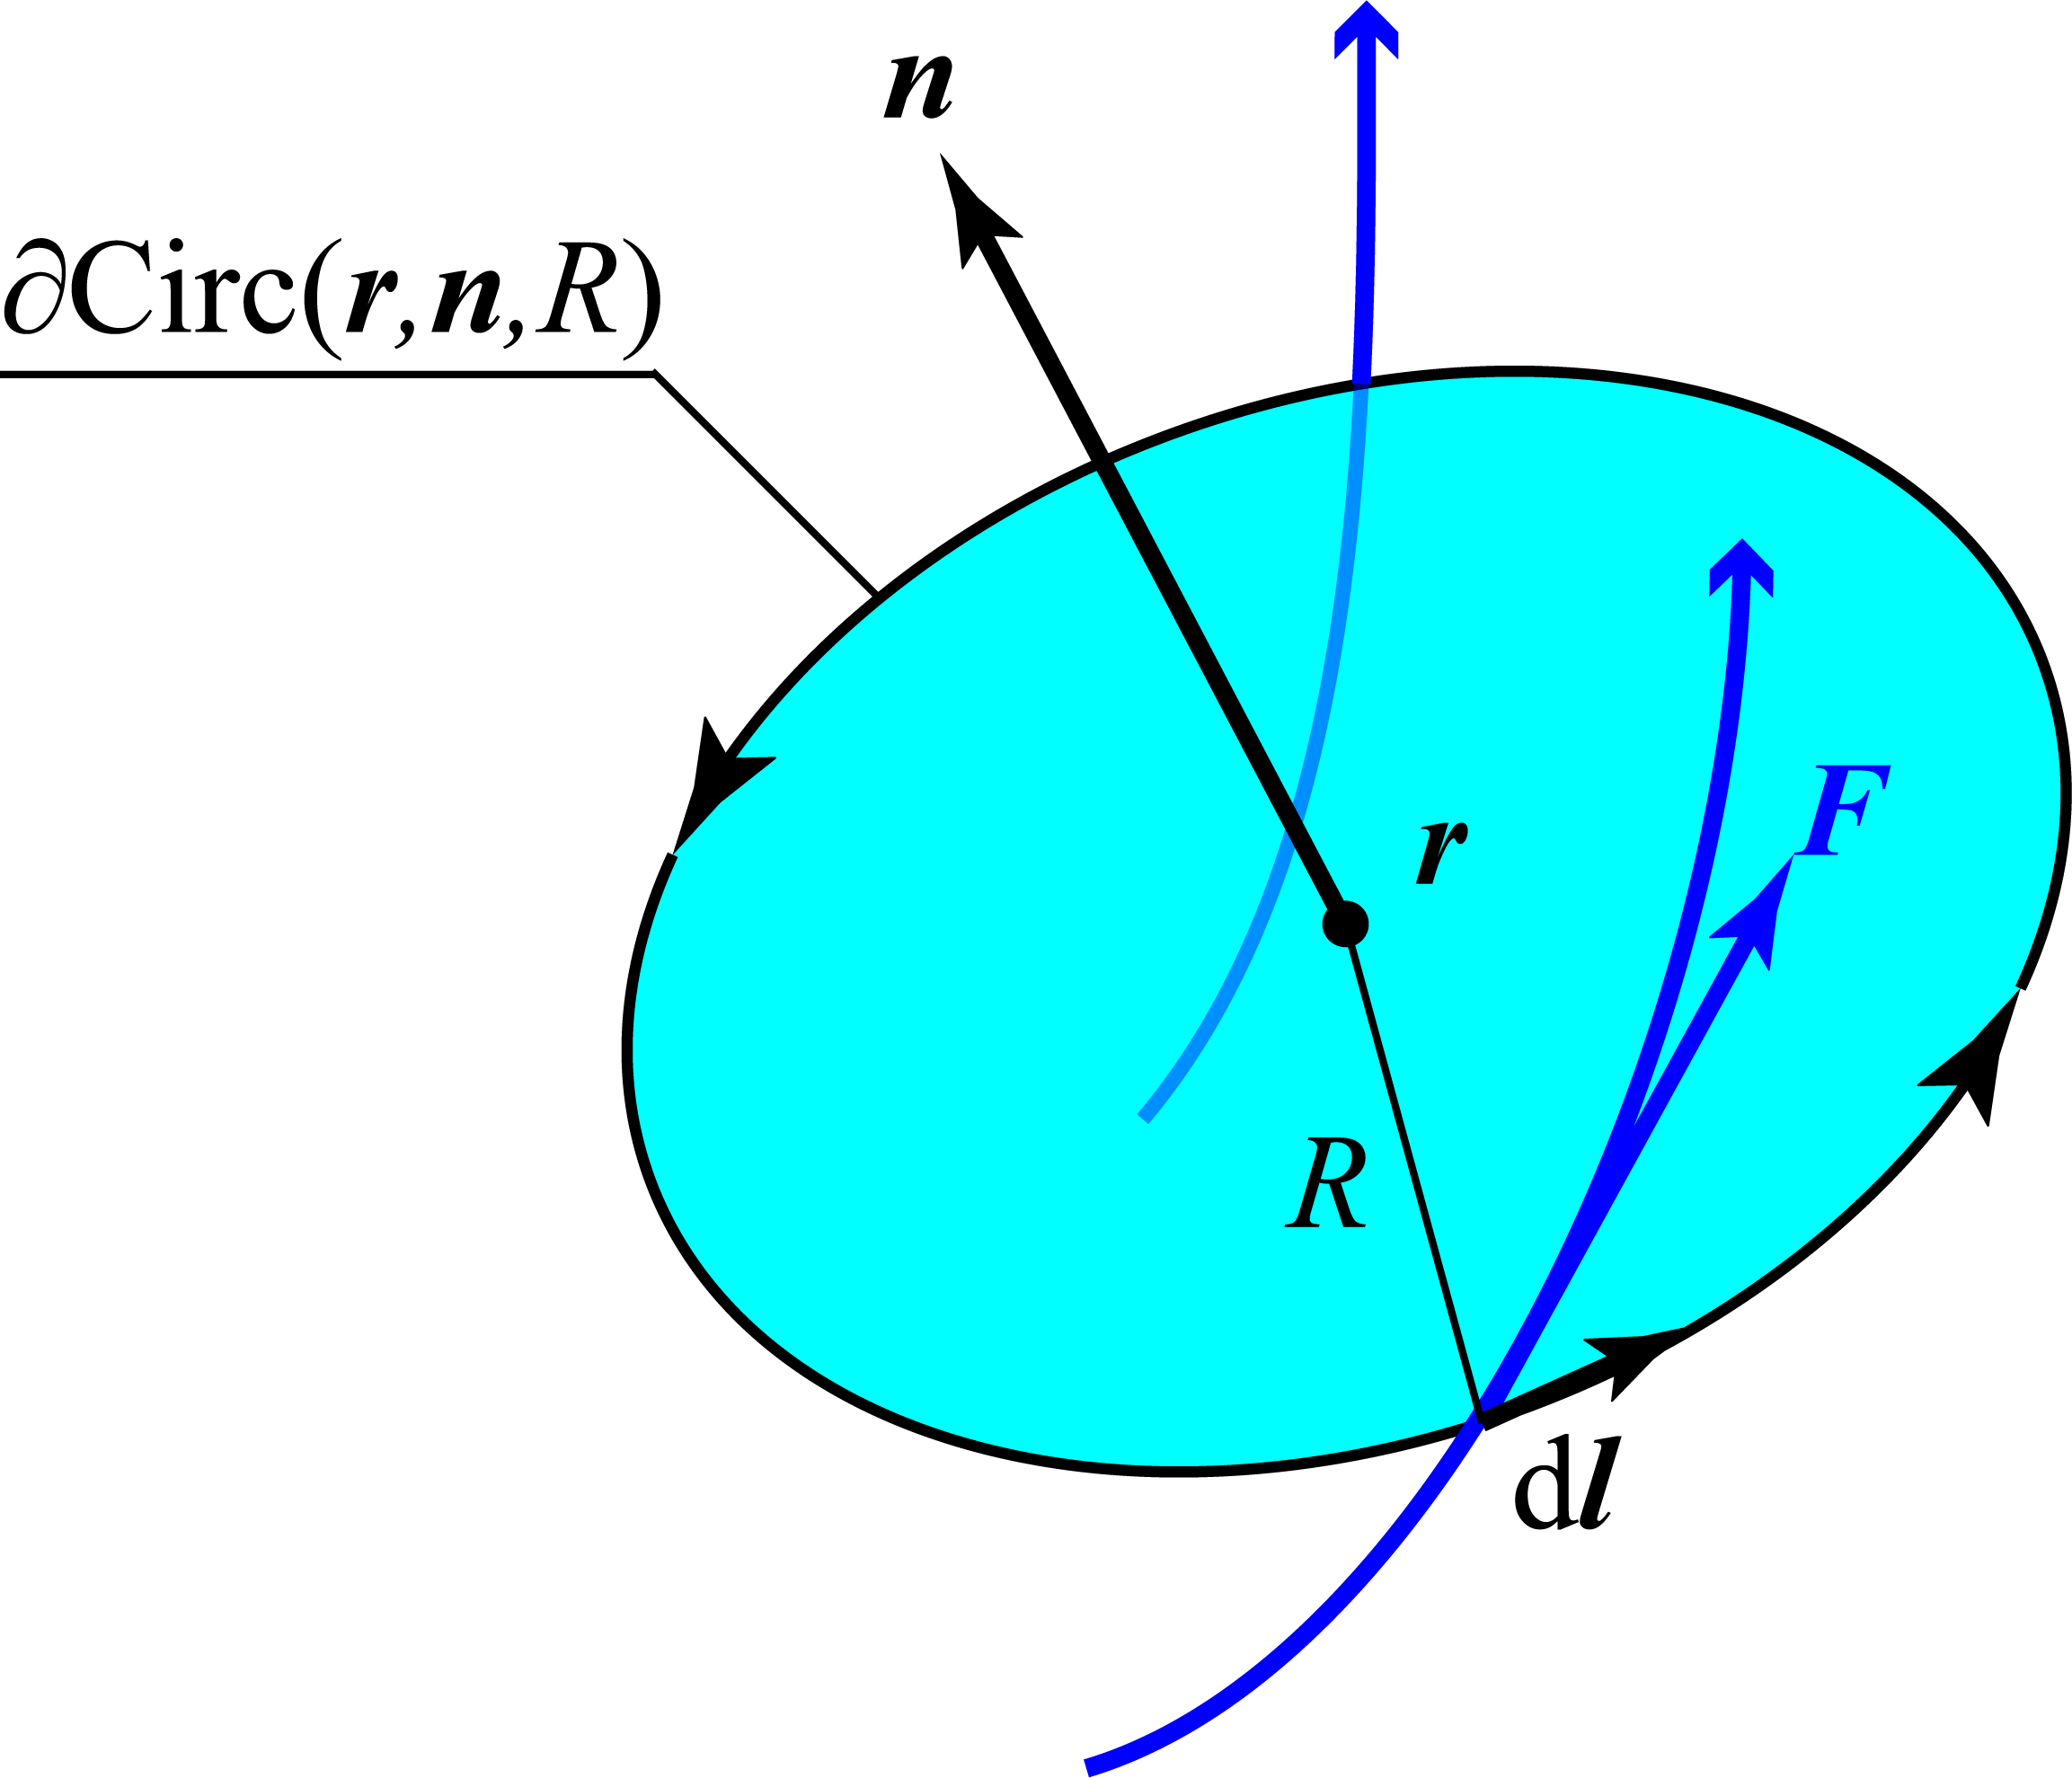
\includegraphics[width=7cm]{image/7-1-5.png}
\caption{矢量场的旋度}
\end{wrapfigure}
第二个概念便是\emph{旋度}(curl)了.\,它实际上代表矢量场的变化矩阵表中反对称的那一部分\footnote{任何一个矩阵都可以被唯一地分解为一个对称矩阵与反对称矩阵之和,\,前者有六个独立分量,\,包含原来的对角线与对称位置的两元素和的一半,\,后者仅有三个独立分量,\,为对称两个位置元素差的一半.}.\,它可以被写为一个矢量.\,与在这一点处的无限小的环积分有关,\,数学上不难证明:
\[\bs{n}\cdot\nabla\times \bs{F}=\lim_{R\to 0}\left.\left(\oint_{\partial {\rm Circ}(\bs{r},\bs{n},R)}\bs{F}\cdot \ud\bs{l}\right)\right/(\pi R^2)\]

由于半径为$R$的圆的选取还依赖于其朝向.\,故在上式中我们对积分的方向和垂直于积分圆面的法向单位矢量$n$采取了右手定则式的对应.\,而最后积分出来得到的数恰好是面法向单位矢量与从$\bs{F}$的各个导数中提取的旋度矢量的点乘.\,环积分通常被称为\emph{环量}(circulation),\,旋度则反应矢量场局域的涡旋程度.\,数学上可以证明旋度可以由行列式表示为:
\[\nabla\times \bs{F}=\begin{vmatrix}
\dfrac{\partial}{\partial x}&\dfrac{\partial}{\partial y}&\dfrac{\partial}{\partial z}\\
F_x&F_y&F_z\\
\bs{e}_x&\bs{e}_y&\bs{e}_z
\end{vmatrix}\]

作为与牛顿-莱布尼茨定理对应的散度与旋度版本,\,根据两个量的定义可知前者发生在体积内部的积分与其闭合表面上,\,后者发生在曲面上面积分和它的闭合曲线边界上:
\[\int\limits_V \nabla\cdot \bs{F}\ud V=\oint\limits_{\partial V}\bs{F}\cdot\ud\bs{A}\]
\[\int\limits_A \nabla\times \bs{F}\cdot\ud \bs{A}=\oint\limits_{\partial A}\bs{F}\cdot\ud\bs{l}\]

前者为\emph{奥斯特诺格拉德斯基-高斯定理}(Ostrogradsky-Gauss theorem),\,后者则为\emph{开尔文-斯托克斯定理}(Kelvin-Stokes theorem)\footnote{微分流形上的微分形式有一个\emph{嘉当-斯托克斯定理}(Cartan-Stokes theorem)统一了以上所有形式:
\[\oint\limits_{\partial \Omega}\omega=\int\limits_\Omega \ud \omega\]}.

现在让我们回到库仑定律,\,现在就必须把它理解为两个公式:
\[\bs{E}=\ke \frac{Q}{r^2}\bs{e}_r\quad ;\quad \bs{F}=q\bs{E}\]

前一半式子说明,\,即使没有引入任何试探电荷$q$,\,在空间中距离场源电荷$Q$为$r$处依然存在某种独立于电荷而存在的``场''.\,否则也就不可能对引入的电荷瞬间产生力的作用.\,这个场由电荷激发,\,以后将知道它有自己的能量与动量,\,而且都是可以被局域地确定\footnote{即,\,可以确定每一点的场能量动量密度.}.\,经典物理中似乎只能由电荷产生场,\,但高能物理下场也能反过来产生电荷粒子,\,实际上此时会将电磁场理解为``光子''这样的物质.\,电磁场的特点是能对带电荷的物质产生作用.

而后一半的式子则给出了电磁场中一点处电场强度矢量$\bs{E}$的定义.\,带电粒子如果在电磁场中静止,\,那么将受到一个与电荷量成正比的力.\,把力与电荷量的比值定义为电场强度矢量.

显然,\,带电粒子的引入也会产生电场.\,这个电场与原来场源电荷产生的电场叠加,\,形成了空间的真实电场分布.\,但在计算这个``试探电荷''的电场时,\,不应该考虑自己在自己这一点处产生的电场.\,因为自己对自己的力总是零.\,而总是计算``外场''在试探电荷这一点的值.\,不过,\,试探电荷的引入与否可能会对外界的场源电荷分部产生改变.\,从而改变外场.\,这又需要另说了,\,我们下一章的导体静电感应就是在不断讨论这个问题.

电场满足\emph{叠加原理}(superposition principle).\,我们总是一对一对地考虑电荷之间的二体作用,\,把相互作用力做非相干的矢量叠加.\,这也就是说,\,给定一个场源电荷分部,\,可以叠加计算出空间中任意一点的电场强度:
\[\bs{E}(\bs{r})=\int\limits_{V'} \ke \frac{\rho \bs{e}_{\bs{R}}}{\bs{R}^2} \ud V'\quad,\quad \bs{R}=\bs{r}-\bs{r}'\]
\[\bs{E}(\bs{r}):=\frac{\bs{F}_{\rm static}}{q}\]

也是出于这个原因,\,所有由电场强度派生出来的量:\,电势,\,电通量等等都符合线性的叠加原理.\,马上就会介绍,\,这是由于描述电场与电荷关系的基本方程是一个线性的微分方程的缘故.




\section{两个定律与电势}

库仑定律是静电学最基本的公理,\,但我们研究电场作为场的性质,\,它与电荷的关系.\,为以后深入了解电磁场整体打好基础.

\subsection{电场的高斯定律}

首先让我们研究\emph{电通量}(electric flux),\,通过一个曲面(不一定闭合)的电通量定义为曲面上电场强度的积分:
\[\varPhi=\int\limits_A \bs{E}\cdot\ud \bs{A}\]

我们在这儿必须引入有向曲线,\,曲面,\,体积的概念.\,固然,\,曲线,\,曲面,\,体积都没有方向与正负,\,它们仅仅是特定空间中的几何形状.\,但定义各种积分时,\,曲线积分的线元矢量$\ud\bs{l}$,\,曲面积分的面元矢量$\ud\bs{A}$都有两个可能的方向.\,而体积元$\ud V$也不一定恒正,\,在某些情况下将取负.\,那么我们通常会有一个符号约定:

\begin{enumerate}
	\item 对于\emph{可定向}(orientable)曲面(不可定向的比如莫比乌斯环),\,总是定义一个方向为正,\,即为每一个面元指定一个面元矢量,\,它取垂直于面的两个方向之一,\,而相邻的面元具有相同的取向.\,而如果涉及到面边界上闭合曲线的环积分,\,则线元矢量取的方向与面元构成\emph{右手定则}(right-hand rule).
	\item 对于\emph{连通}(connected)体积区域,\,如果取体积微元为正,\,那么涉及到区域边界闭合曲面上的面积分时,\,面元取从体积内到体积外的方向.\,如果取体积微元为负,\,则面上面元取体积外到体积内的方向.
\end{enumerate}

而我们之前写出的奥-高定理和开-斯定理,\,都是在这个意义下正确的.

从而以上电通量也就因为我们选择的面的两种可能的正向而造成两个不同的结果,\,它们相差一个相反数.

电场的\emph{高斯定律}(Gauss's law)指出:
\[\varPhi_{\partial V}=\oint\limits_{\partial V} \bs{E}\cdot\ud \bs{A}=\frac{1}{\varepsilon_0}\int\limits_V \rho\ud V\]

\begin{figure}[H]
\centering
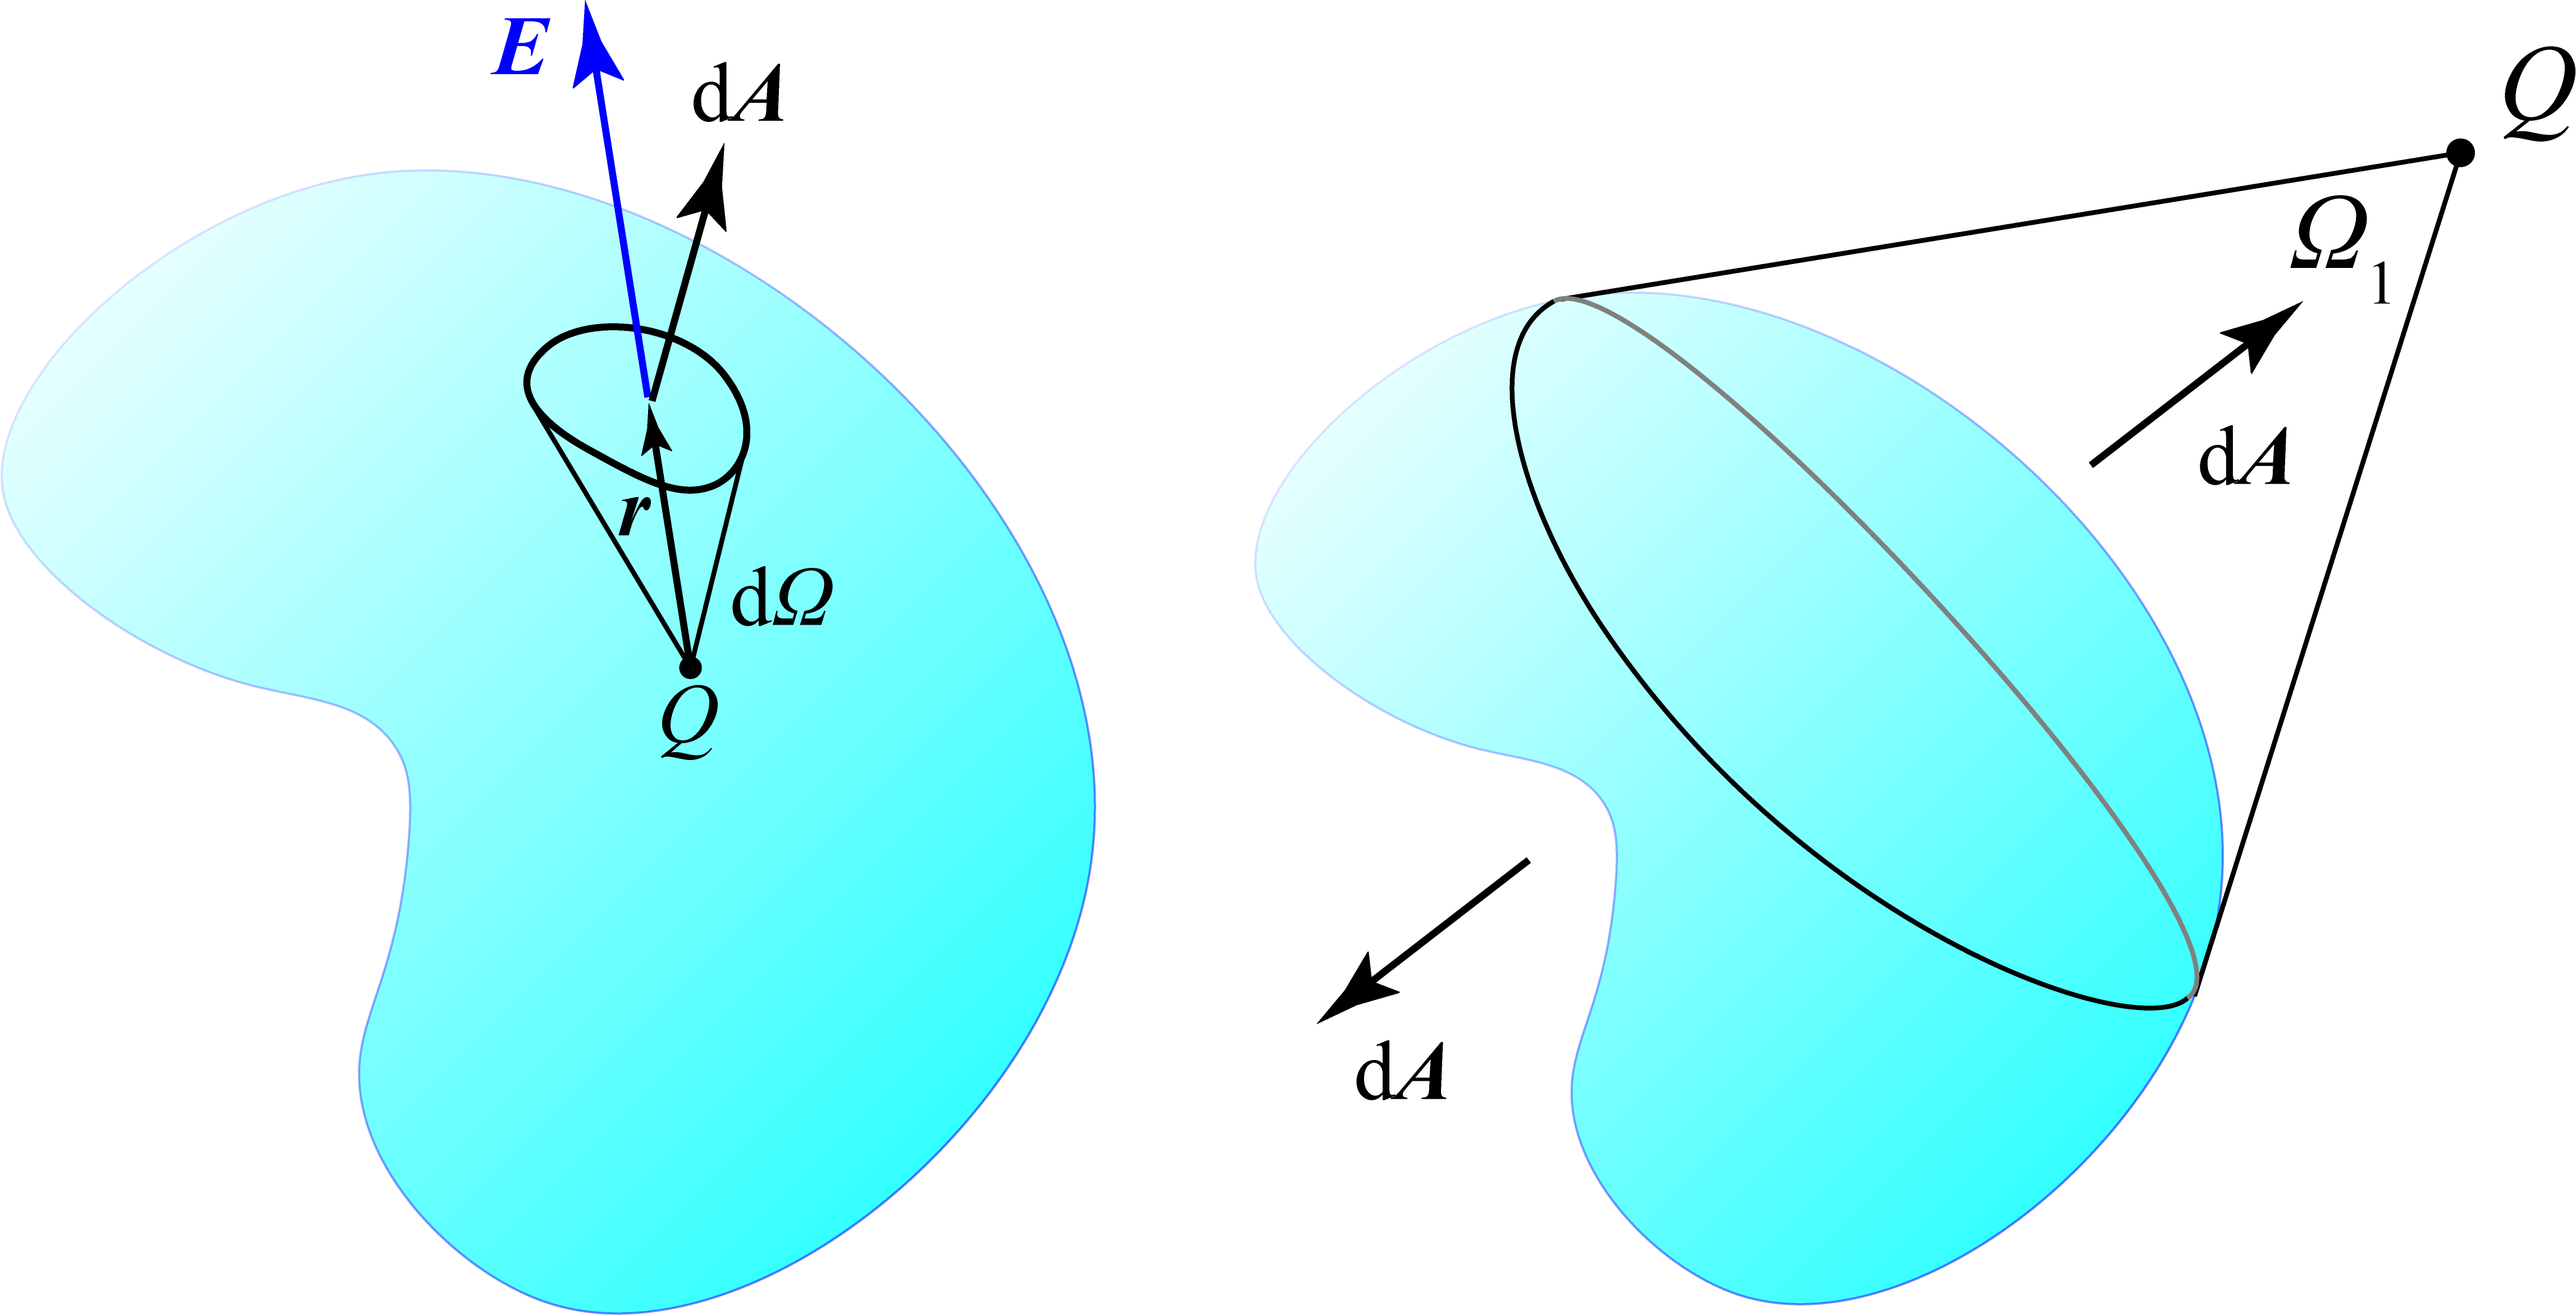
\includegraphics[width=0.5\textwidth]{image/7-1-6.png}
\caption{证明高斯定律}
\end{figure}

我们来用库仑定律证明高斯定律.\,首先考虑一个在闭合曲面内部的点电荷,\,我们发现面元上的通量:
\[\ud \varPhi=\bs{E}\cdot\ud \bs{A}=\ke \frac{Q\bs{e}_{\bs{r}}\cdot\ud \bs{A}}{\bs{r}^2}\]

而这一个小面元对点电荷张的立体角恰好是:
\[\ud\varOmega=\frac{\bs{e}_{\bs{r}}\cdot\ud \bs{A}}{\bs{r}^2}\]

故对面积分总立体角给出$4\pi$的结果:
\[\ud \varPhi=\frac{Q}{\varepsilon_0}\cdot\frac{\ud\varOmega}{4\pi}\quad \Rightarrow\quad \varPhi=\frac{Q}{\varepsilon_0}\cdot\oint\limits_{\partial V}\frac{\ud\varOmega}{4\pi}=\frac{Q}{\varepsilon_0}\]

我们再考虑在面外的点电荷$Q$对面产生的电通量,\,此时面的正向与点电荷产生电场方向的点乘就有了正负号,\,积分以后得到的结果是通过点电荷去看曲面,\,把曲面对点电荷张的最大视角处的曲线找到,\,将曲面分为两个部分,\,立体角都是$\varOmega_1$,\,总积分为:
\[\varPhi=\frac{Q}{\varepsilon_0}\cdot\oint\limits_{\partial V}\frac{\ud\varOmega}{4\pi}=\frac{Q}{\varepsilon_0}(\varOmega_1-\varOmega_1)=0\]

从而我们证明了,\,电荷若在闭合曲面内,\,则电通量贡献为\(\frac{Q}{\varepsilon_0}\).\,而若在闭合曲面外,\,则电通量贡献为$0$.\,再由叠加原理,\,得任意情况下闭合曲面的电通量等于内部总电荷量除真空介电常数$\varepsilon_0$.\,考虑电荷连续分布或准连续分布的情况下,\,有:
\[\oint\limits_{\partial V} \bs{E}\cdot\ud \bs{A}=\frac{1}{\varepsilon_0}\int\limits_V \rho\ud V\]

此即高斯定律,\,由数学上的奥-高定理,\,我们可以把上式写为局域的微分形式:
\[\nabla\cdot\bs{E}=\frac{\rho}{\varepsilon_0}\]

高斯定律旨在说明:\,电荷产生电场(电荷是电场的源强度).

\subsection{电势与电场的环路定律}

对点电荷产生的电场$\bs{E}=\dfrac{Q}{4\pi\varepsilon_0 r^2}\bs{e}_r$,\,再引入以下标量场是方便的:
\[\varphi=\ke\frac{Q}{r}\]

这是因为如果计算球坐标下的梯度:
\[\nabla=\bs{e}_r\frac{\partial}{\partial r}+\frac{\bs{e}_\theta}{r}\frac{\partial}{\partial \theta}+\frac{\bs{e}_\varphi}{r\sin\theta}\frac{\partial}{\partial \varphi}\]

便得到以下关系式:
\[\bs{E}=-\nabla\varphi\]

即电场可以表示为我们引入的另一个标量场的负梯度的形式.\,这个标量场就叫做\emph{电势}(electric petential).\,而以上关系,\,结合梯度的含义理解,\,便是沿电场线方向电势降低.\,可以通过牛-莱定理写为积分形式(下式与路径无关):
\[\int_A^B \bs{E}\cdot \ud\bs{l}=\varphi_A-\varphi_B\]

以上关系式由叠加原理,\,在任意电荷分部的情况下都成立,\,此时对应的电势标量场为:
\[\varphi(\bs{r})=\int \ke\frac{\rho}{|\bs{R}|}\ud V'\quad ,\quad \bs{R}=\bs{r}-\bs{r}'\]

对于电势的引入可能存在一点疑惑:\,我们都知道电场的定义是可以独立于场源电荷的,\,它为在一点处引入静止的试探电荷时单位电荷的受力.\,那么电势是否可以独立于场源电荷而定义呢?\,观点一比较基础,\,它认为在静电场情况下既然全空间电场已经被定义了,\,它就应该反映了该点处场的全部实际信息,\,那么电势作为与电场符合一个梯度关系的梯度场,\,也就能被相应的确定下来,\,两个可能的电势还可以差一个全空间都一致的常数.\,也就是这种观点把电场视为更加基础的场的特征.\,下面便可以知道电势的含义是引入试探电荷后单位试探电荷在该点处的电势能.\,而观点二则更加本质,\,我们今天知道了势比场强实际上包含更多的信息.\,由于微观粒子的量子特性,\,力的概念已然失效,\,从而场强反而不如用势来描述一个场更为直接而实用.\,电磁场论实际上也就是一个是矢量场论,\,它由矢势和标势组成一个四维矢量来完整地描述,\,但取法不唯一,\,多出来的冗余自由度被称为\emph{规范}(gauge),\,它恰好就在表示电荷与场的相互作用时,\,与电荷的量子相位协同变化,\,从而造成实际可以观测的影响.\,为了实际问题的方便,\,通常约定势有特定的取法.\,在静电学的常见情况下(电荷分布区域有限时),\,常常取无穷远处电势为零,\,注意上电势积分式也恰恰符合这一点.

我们进一步考察电势的物理含义,\,如果把以上电场视为外电场,\,引入试探电荷$q$,\,并在以上积分形式的场强与势的关系中乘以$q$,\,便发现$q\bs{E}$就是电荷的受力,\,左边就是表示电场力的做功:
\[W_{A\to B}=q\varphi_A-q\varphi_B\]

很自然地我们发现电场力是保守力,\,而对应的电势能,\,基于它应该与电荷量成正比的观点,\,我们总是直接取为:
\[E_p=q\varphi\]

从而电势的效果,\,是为试探电荷带来一个电势能.

最后我们再考察电场的一个特性,\,由于任何路径上的电场积分可以根据牛-莱定理写为端点的电势差的形式,\,考虑闭合的曲线积分,\,它可以看成一个可定向曲面的边界,\,由于两端点重合:
\[\oint\limits_{\partial A}\bs{E}\cdot\ud \bs{l}=0\]

这就是电场的\emph{环路定律}(circuital law),\,再根据数学上的开-斯定理,\,我们写出环路定律的微分形式:
\[\nabla\times\bs{E}=\bs{0}\]

也就是静电场无旋.\,值得指出这不过是静电场可以表示为标量电势场的负梯度的直接结果,\,因为任意一个标量场的梯度都是无旋的\footnote{这个结论向流形推广就是著名的\emph{庞加莱引例}(Poincar'e lemma)了,\,它指出任意$p-$形式$\omega$的二次全微分为零:
\[\ud\ud\omega=0\]

一个以后会用得上的推论可以通过考察矢量场的旋度在闭合曲面上的面积分,\,而把闭合曲面看成是边界曲线缩小到零的有边界曲面而得:
\[\oint\limits_{\partial V}\nabla \times \bs{F}\cdot\ud \bs{A}=0\quad \Rightarrow \quad \nabla\cdot\nabla \times\bs{F}=0\]}:
\[\oint\limits_{\partial A}\nabla f\cdot\ud \bs{l}=0\quad \Rightarrow \quad \nabla\times\nabla f=\bs{0}\]

\subsection{总结}

\begin{wrapfigure}[9]{o}[0pt]{8cm}
\centering
\vspace{-0.1cm}
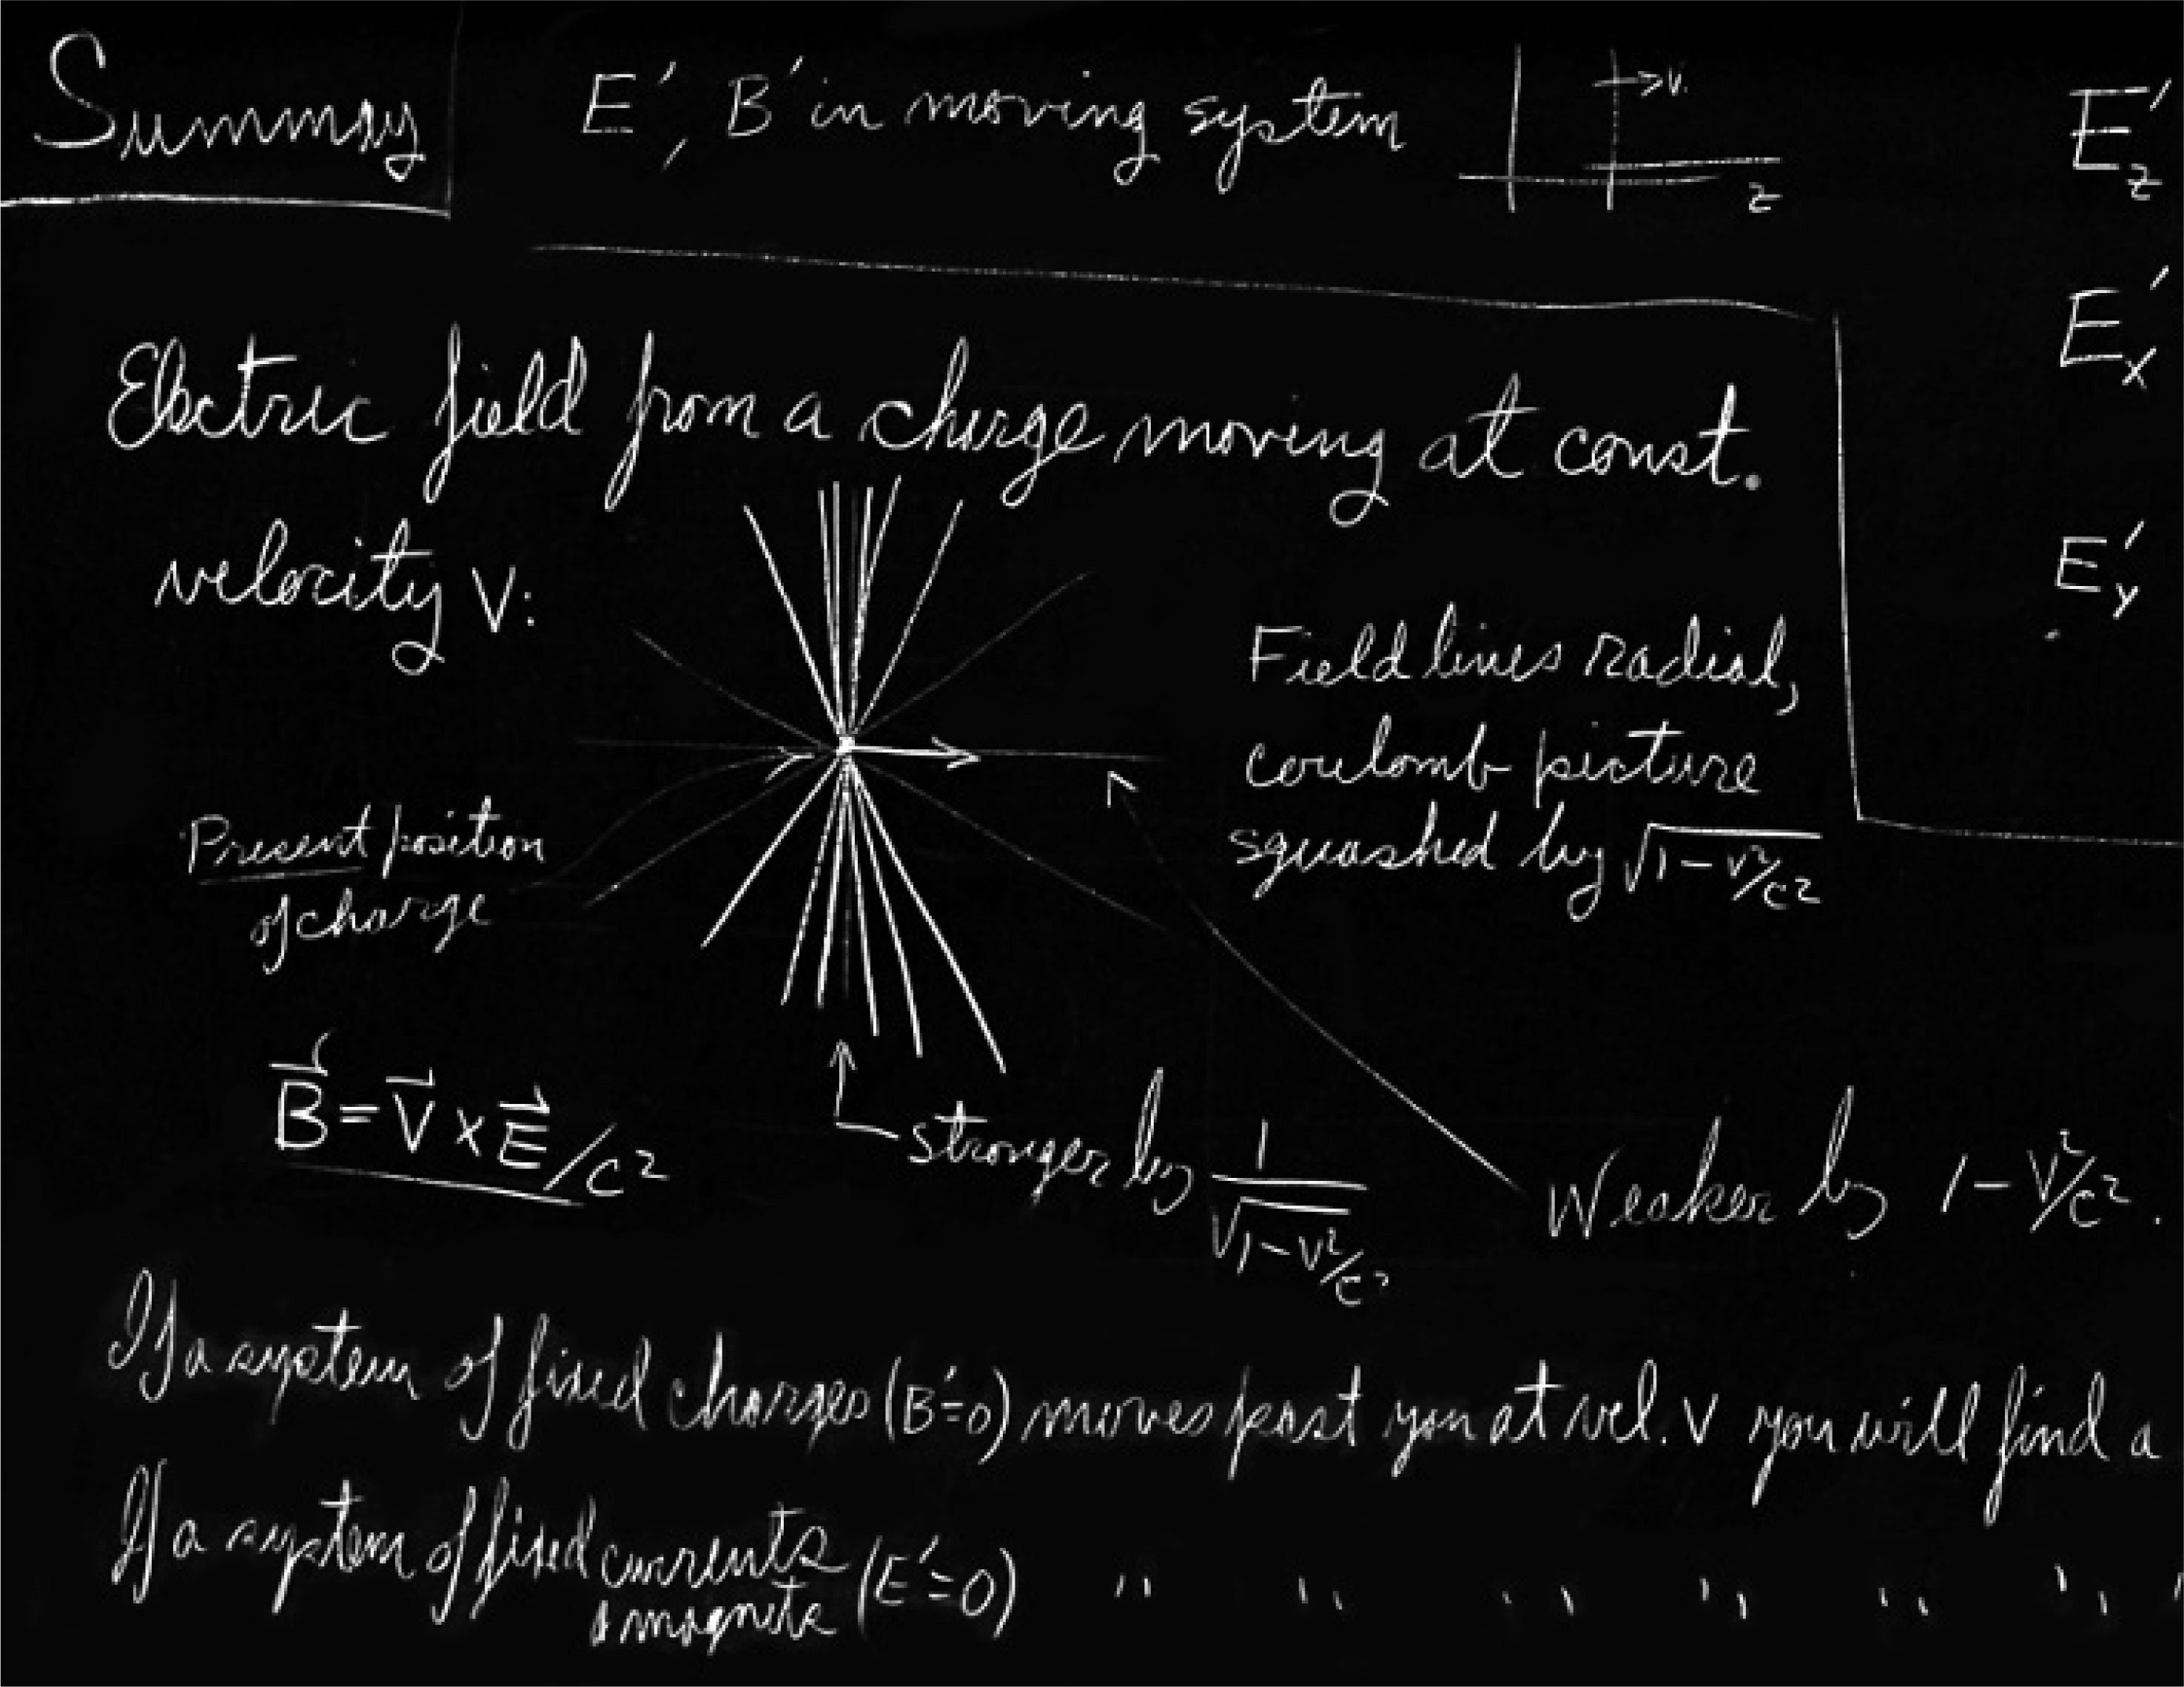
\includegraphics[width=8cm]{image/7-1-7.png}
\caption{Feynman讲座一瞥}
\end{wrapfigure}
我们现在有三个不同的层次去看待电荷与电荷之间的相互作用问题\footnote{拉普拉斯算子$\nabla^2=\nabla\cdot\nabla$,\,如作用在标量上即表示先求梯度后求散度:
	\[\nabla^2f=\nabla\cdot(\nabla f)\]}:
\begin{description}
	\item[{\hei 1. 不引入场:}]

	\[\bs{F}=\ke\frac{Qq}{r^2}\bs{e}\]

	\item[{\hei 2. 引入场,\,用场强描述:}]

	\[\nabla\cdot \bs{E}=\frac{\rho}{\varepsilon_0}\quad ;\quad \nabla\times\bs{E}=\bs{0}\]
	\[\bs{F}=q\bs{E}\]

	\item[{\hei 3. 引入场,\,用势描述:}]
	\[\nabla^2 \varphi=-\frac{\rho}{\varepsilon_0}\]
	\[E_p=q\varphi\]
\end{description}


以上描述一个比一个适用范围更广,\,第一个仅仅适用于静电场或低速情况,\,第二个则是对高速运动的电荷与电磁场适用,\,比如匀速运动的电荷的场强由简单相对论讨论可得:
\[\bs{E}=\ke\frac{Q}{r^2}\frac{1-\beta^2}{(1-\beta^2\sin^2\theta)^{3/2}}\bs{e}_r\]
\[\bs{B}=\frac{\bs{v}\times\bs{E}}{c^2}\]

它要符合第二个式子(旋度需要做相对论修正),\,而第三个式子更是适用于非经典场论情况.


\section{静电能}

我们将进一步深入研究电场相互作用中的能量概念.

\subsection{静电势能}

\begin{wrapfigure}[13]{o}[0pt]{8cm}
\centering
\vspace{-0.1cm}
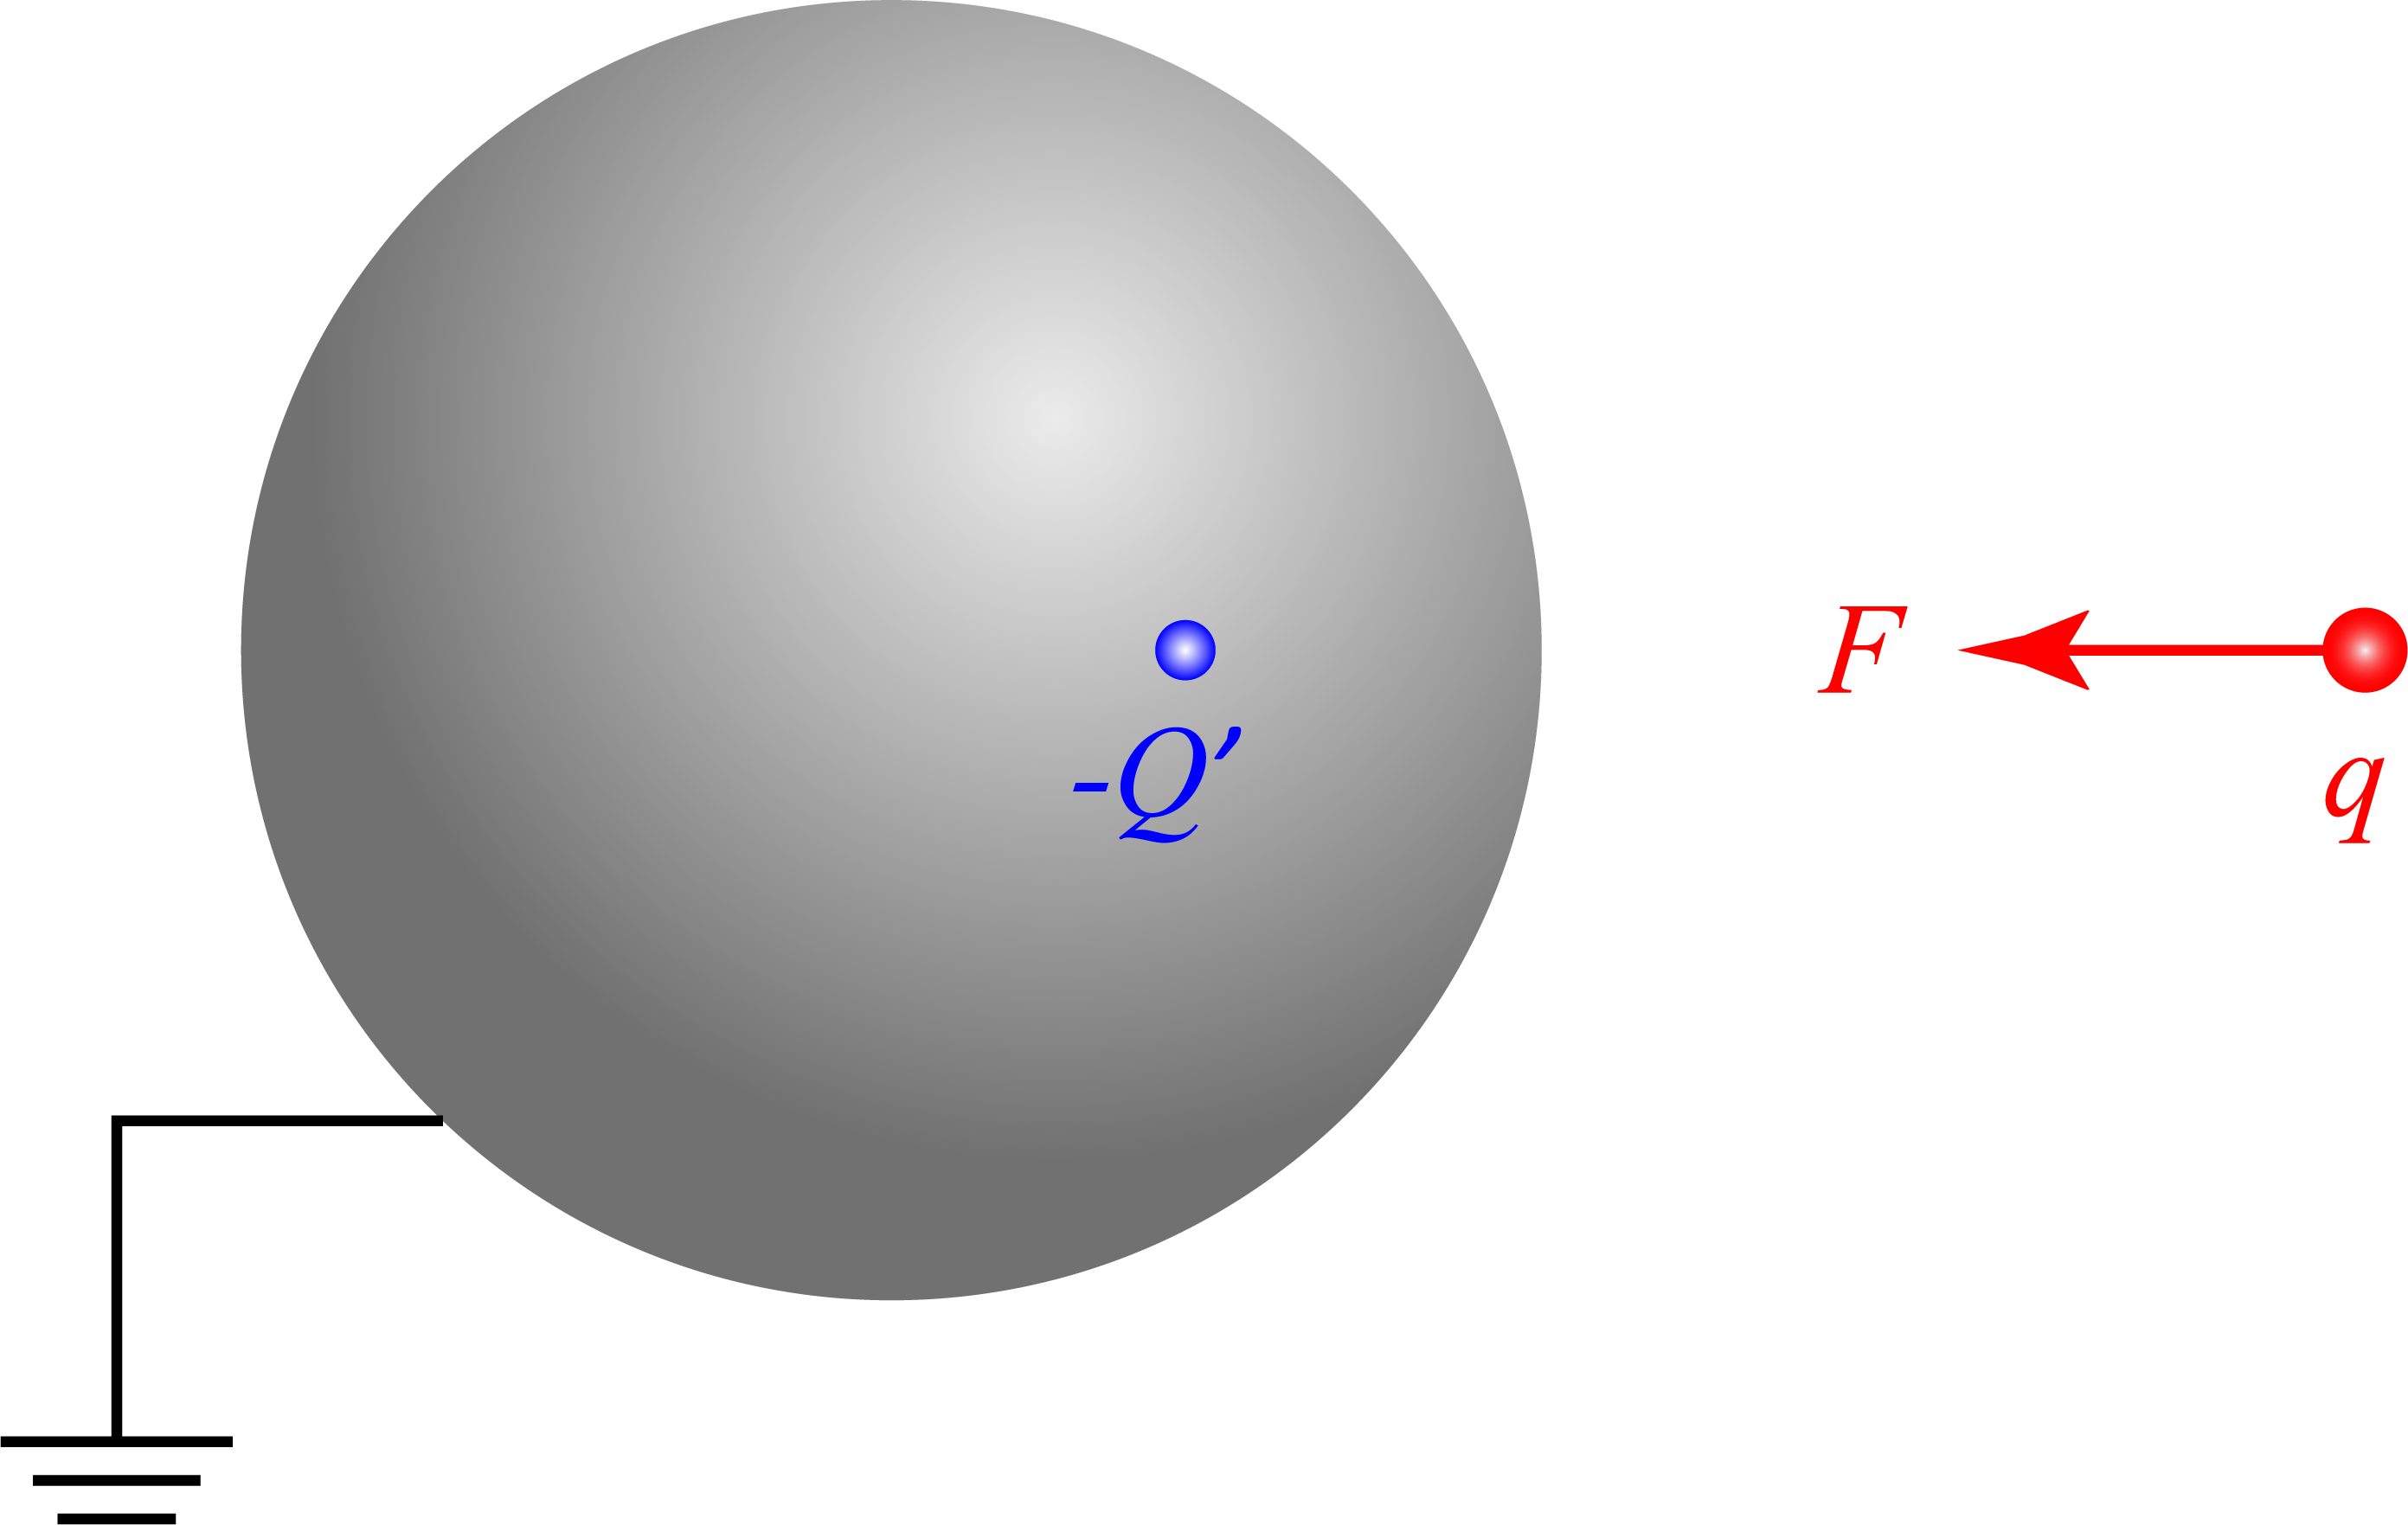
\includegraphics[width=8cm]{image/7-1-8.png}
\caption{情形:\,场源电荷取决于试探电荷}
\end{wrapfigure}
之前已经引入了电势能的概念,\,我们把外场中引入的试探电荷(点电荷)所具有的势能的大小计做电势能,\,并得出了电势能的表达式:
\[E_p=q\varphi\]

还指出了,\,它的作用是用来表示不变的外电场对电荷的做功的多少,\,基于这样的观察,\,我们把这个能量称为\emph{静电势能}(electrostatic potential energy),\,静电的含义,\,是要求外场不能随着试探电荷的引入与移动而改变.\,而更常见的一类情况是,\,随着试探电荷的移动,\,场源电荷也在随着改变,\,如之后将会经常讨论的静电感应的情况.\,此时仍然可以计算外场的场强与电势,\,并引入试探电荷以后依然可以形式地写出\emph{电势能}(electro potential energy)的值$E_p=q\varphi$,\,但它不再代表实际移动试探电荷电场对电荷做的功了,\,它代表什么?\,电场对电荷做功普遍地应该怎么表示?\,外力做功又如何和它发生联系,\,这是我们之后的讨论关心的问题.

首先对于这个问题的第一步考察是,\,虽然试探电荷的特定位置带来特定的外场,\,但一旦确定了外场的场源的电荷分布,\,便可以独立于试探电荷地产生一个分布于全空间的电势与电场,\,而可以设想固定这个电荷分布不变,\,而把试探电荷放在空间中的任意一点,\,讨论其受力与能量.\,这些改变试探电荷位置而不改变外场的位移称为\emph{虚位移}(virtual displacement).\,它是一种广泛用来建立理论模型的方法.\,它的强大之处在于虚位移的任意性,\,在每一个实际时刻试探电荷可以在任意位置,\,外场在缓慢随时间发生改变,\,而试探电荷发生的实际位移是所有虚位移中的一个特例.\,在这个意义下,\,电势能的含义便在于,\,试探电荷发生虚位移时,\,即场源电荷分布不变时,\,电场力对试探电荷做的虚功即为电势能的减小,\,此即静电场下的虚功原理:
\[\delta E_p=-q\bs{E}\cdot\delta \bs{r}\]

我们可以把这个概念推广,\,如果在该外场中引入不止一个点试探电荷,\,我们写出一个电荷体系在外场中的电势能来:
\[E_p=\sum_i q_i\varphi_i\]

这个写法存在一些问题,\,首先是如果没有引入任何试探电荷,\,体系是否固有一个能量?\,用场的角度来理解就会发现不对,\,场是一种物质,\,物质必定伴随着能量.\,或者考虑场源电荷之间的相互作用,\,它也一定会伴随着能量.\,再者,\,引入两个以上的点电荷时,\,它们之间的相互作用能没有被包含在以上项中.\,第三,\,即使是单个点电荷单独存在,\,也必定会带来其自能.\,我们需要从更基础的角度来讨论电荷体系的能量.




\subsection{自能与相互作用能}

考虑真空中的两个点电荷之间的相互作用.\,电荷$q_1$在电荷$q_2$处产生的电场与电势为$\bs{E}_{12}$与$\varphi_{12}$,\,电荷$q_2$在电荷$q_1$处产生的电场与电势为$\bs{E}_{21}$与$\varphi_{21}$无疑,\,相互作用力是相互的,\,满足牛顿第三定律$q_1\bs{E}_{21}+q_2\bs{E}_{12}=\bs{0}$.\,那么电势能是相互的吗?\,注意到:
\[q_1U_{21}=\ke\frac{q_1q_2}{r}=q_2U_{12}\]

从而两个电势能实际上是相等的.\,根据电势能的定义,\,它等于$1$不动$2$移到无穷远电场力所做的功,\,也会等于$2$不动$1$移到无穷远电场力所做的功.\,这两种情况平移对称,\,从而我们有理由判断:\,无论如何移动两个电荷,\,将$1$与$2$分开到无限远时电场力做功都会是以上值,\,这一点也不难在数学上证明.

从而我们把这个能量称为$12$间相互作用力对应的\emph{相互作用能}(interaction energy).\,它可以用任何一个电荷乘以另一个电荷在这个电荷处产生的势相乘得到,\,或者找到这一对相互作用,\,直接写出:
\[I_{12}=\ke\frac{q_1q_2}{r_{12}}\]

按照这思路,\,由叠加原理,\,我们可以很轻易地写出点电荷体系与连续分布电荷体系的总相互作用能:
\begin{description}
	\item[{\hei 1. 点电荷体系:}]
	\[I=\sum_{\{i,j\}!} \ke\frac{q_iq_j}{r_{ij}}\]
	\item[{\hei 2. 连续分布电荷体系:}]
	\[I= \iint\limits_{\{\ud V,\ud V'\}!}\ke\frac{\rho\rho'}{r}\ud V\ud V'\]
\end{description}

关于以上求和我们做出以下解释:

首先,\,点电荷体系的相互作用能表示把点电荷从计算这个能量的状态移动到点电荷彼此之间都相距无穷远时电场力所做的功.\,但一定要注意每个点电荷移动到无穷远以后还会因为自身的电磁相互作用而产生一个待定的能量,\,叫做自能,\,我们紧接着会讨论到这个问题.\,而连续分布电荷体系则表示把每一份电荷微元移动到无穷远以后电场力做的功,\,移动到无穷远以后电荷无限分散(宏观意义上),\,所以每一份微元电荷对应的电磁相互作用能真实地趋于零,\,故我们计算的这个能量就是这个体系的总电磁相互作用对应的能量.

第二,\,是这个求和表示的含义.\,我们用$(i,j)$来表示特定集合中两个元素$i,j$构成的\emph{有序对}(ordered pair),\,而$\{i,j\}$则表示交换$i,j$后表示同一代数元素的\footnote{以后还会用到$n$个元素的\emph{对称无序类}(symmetrized unordered setoid)与\emph{反对称无序类}(antisymmetrized unordered setoid):
\[\{i_1\cdots i_p\cdots i_q\cdots i_n\}=\{i_1\cdots i_q\cdots i_p\cdots i_n\}\]
\[[i_1\cdots i_p\cdots i_q\cdots i_n]=-[i_1\cdots i_q\cdots i_p\cdots i_n]\]
}\emph{对称无序对}(symmetrized unordered pair),\,即$\{i,j\}=\{j,i\}$.\,求和下加这个对符号表示对所有一对一对的情况进行求和.\,每一对只需要求一次即可.\,这之后还跟着一个感叹号,\,它表示$i,j$必须取不同值(而$\ud V$与$\ud V'$可以取相同值,\,这些项会在体积很小时求和也很小而可以忽略).\,那么由简单的代数变形,\,我们发现上两式即:
\[I=\frac{1}{2}\sum_i\sum_{j\neq i}\ke\frac{q_iq_j}{r_{ij}}=\frac{1}{2}\sum_iq_i\phi_i\]
\[I=\frac{1}{2}\int\limits_{\ud V}\int\limits_{\ud V'}\ke\frac{\rho\rho'}{r}\ud V\ud V'=\frac{1}{2}\int\limits_{\ud V}\rho \varphi \ud V\]

注意到第一式中$\phi_i$表示的是别的电荷在$q_i$处产生的电势,\,不包括自己在自己上产生的,\,我们把符号稍微变动一下以示区别.\,而在后一个表达式中则不需要考虑这种区别,\,这个式子将作为一个普遍的求总电磁相互作用能的表达式而使用.

第三,\,是这个求和的使用方法.\,实际上,\,如果电荷连续分布系统从一个状态变化到另一个状态,\,电荷分布与它产生的电势分布都发生改变,\,那么前后的能量增加:
\[\Delta I=\frac{1}{2}\int\rho' \varphi' \ud V-\frac{1}{2}\int\rho \varphi \ud V\]

自然表示电场对电荷体系所做的负功,\,或者表示由电荷流向电场的能量,\,它使得场的能量,\,也就是$I$,\,发生了增长\footnote{场只能和带荷的物质发生作用,\,这也是唯一的使得场能量变化的方法}.\,而反过来考察电荷体系,\,如果外力对电荷体系做功为$W$,\,那么根据动能定理应该有:
\[W-\Delta I=\Delta E_k\]

在十分缓慢地移动电荷的情况下,\,亦或是导体在载流子为电子,\,其动能十分的小可以忽略的情况下,\,动能的增长可以视为零,\,从而有:
\[W=\Delta I\]

即,\,外力做功,\,通过电荷为媒介,\,转化为了场的能量的增长.\,这个观点也是我们经常用的到的.

我们最后回到电势能与相互作用能的关系,\,考虑整个体系由两部分电荷体系构成,\,那么由叠加原理,\,整个空间中每一点的电势可以写成两部分贡献的和$\varphi_1+\varphi_2$.\,我们只需要对全空间的电荷积分,\,就得到了整个体系的相互作用能:
\begin{align*}
I 	&=\frac{1}{2}\int\limits_{\rm I+II}\rho \varphi \ud V \\
	&=\frac{1}{2}\int\limits_{\rm I}\rho_1 (\varphi_1+\varphi_2)\ud V_1 + \frac{1}{2}\int\limits_{\rm II}\rho_2 (\varphi_1+\varphi_2)\ud V_2 \\
	&=\frac{1}{2}\int\limits_{\rm I}\rho_1 \varphi_1\ud V_1+\frac{1}{2}\int\limits_{\rm II}\rho_2 \varphi_2\ud V_2+\frac{1}{2}\left(\int\limits_{\rm I}\rho_1 \varphi_2\ud V_1+\int\limits_{\rm II}\rho_2 \varphi_1\ud V_2\right) \\
	&=I_1+I_2+I_{12}
\end{align*}

\begin{wrapfigure}[14]{o}[0pt]{9cm}
\centering
\vspace{-0.1cm}
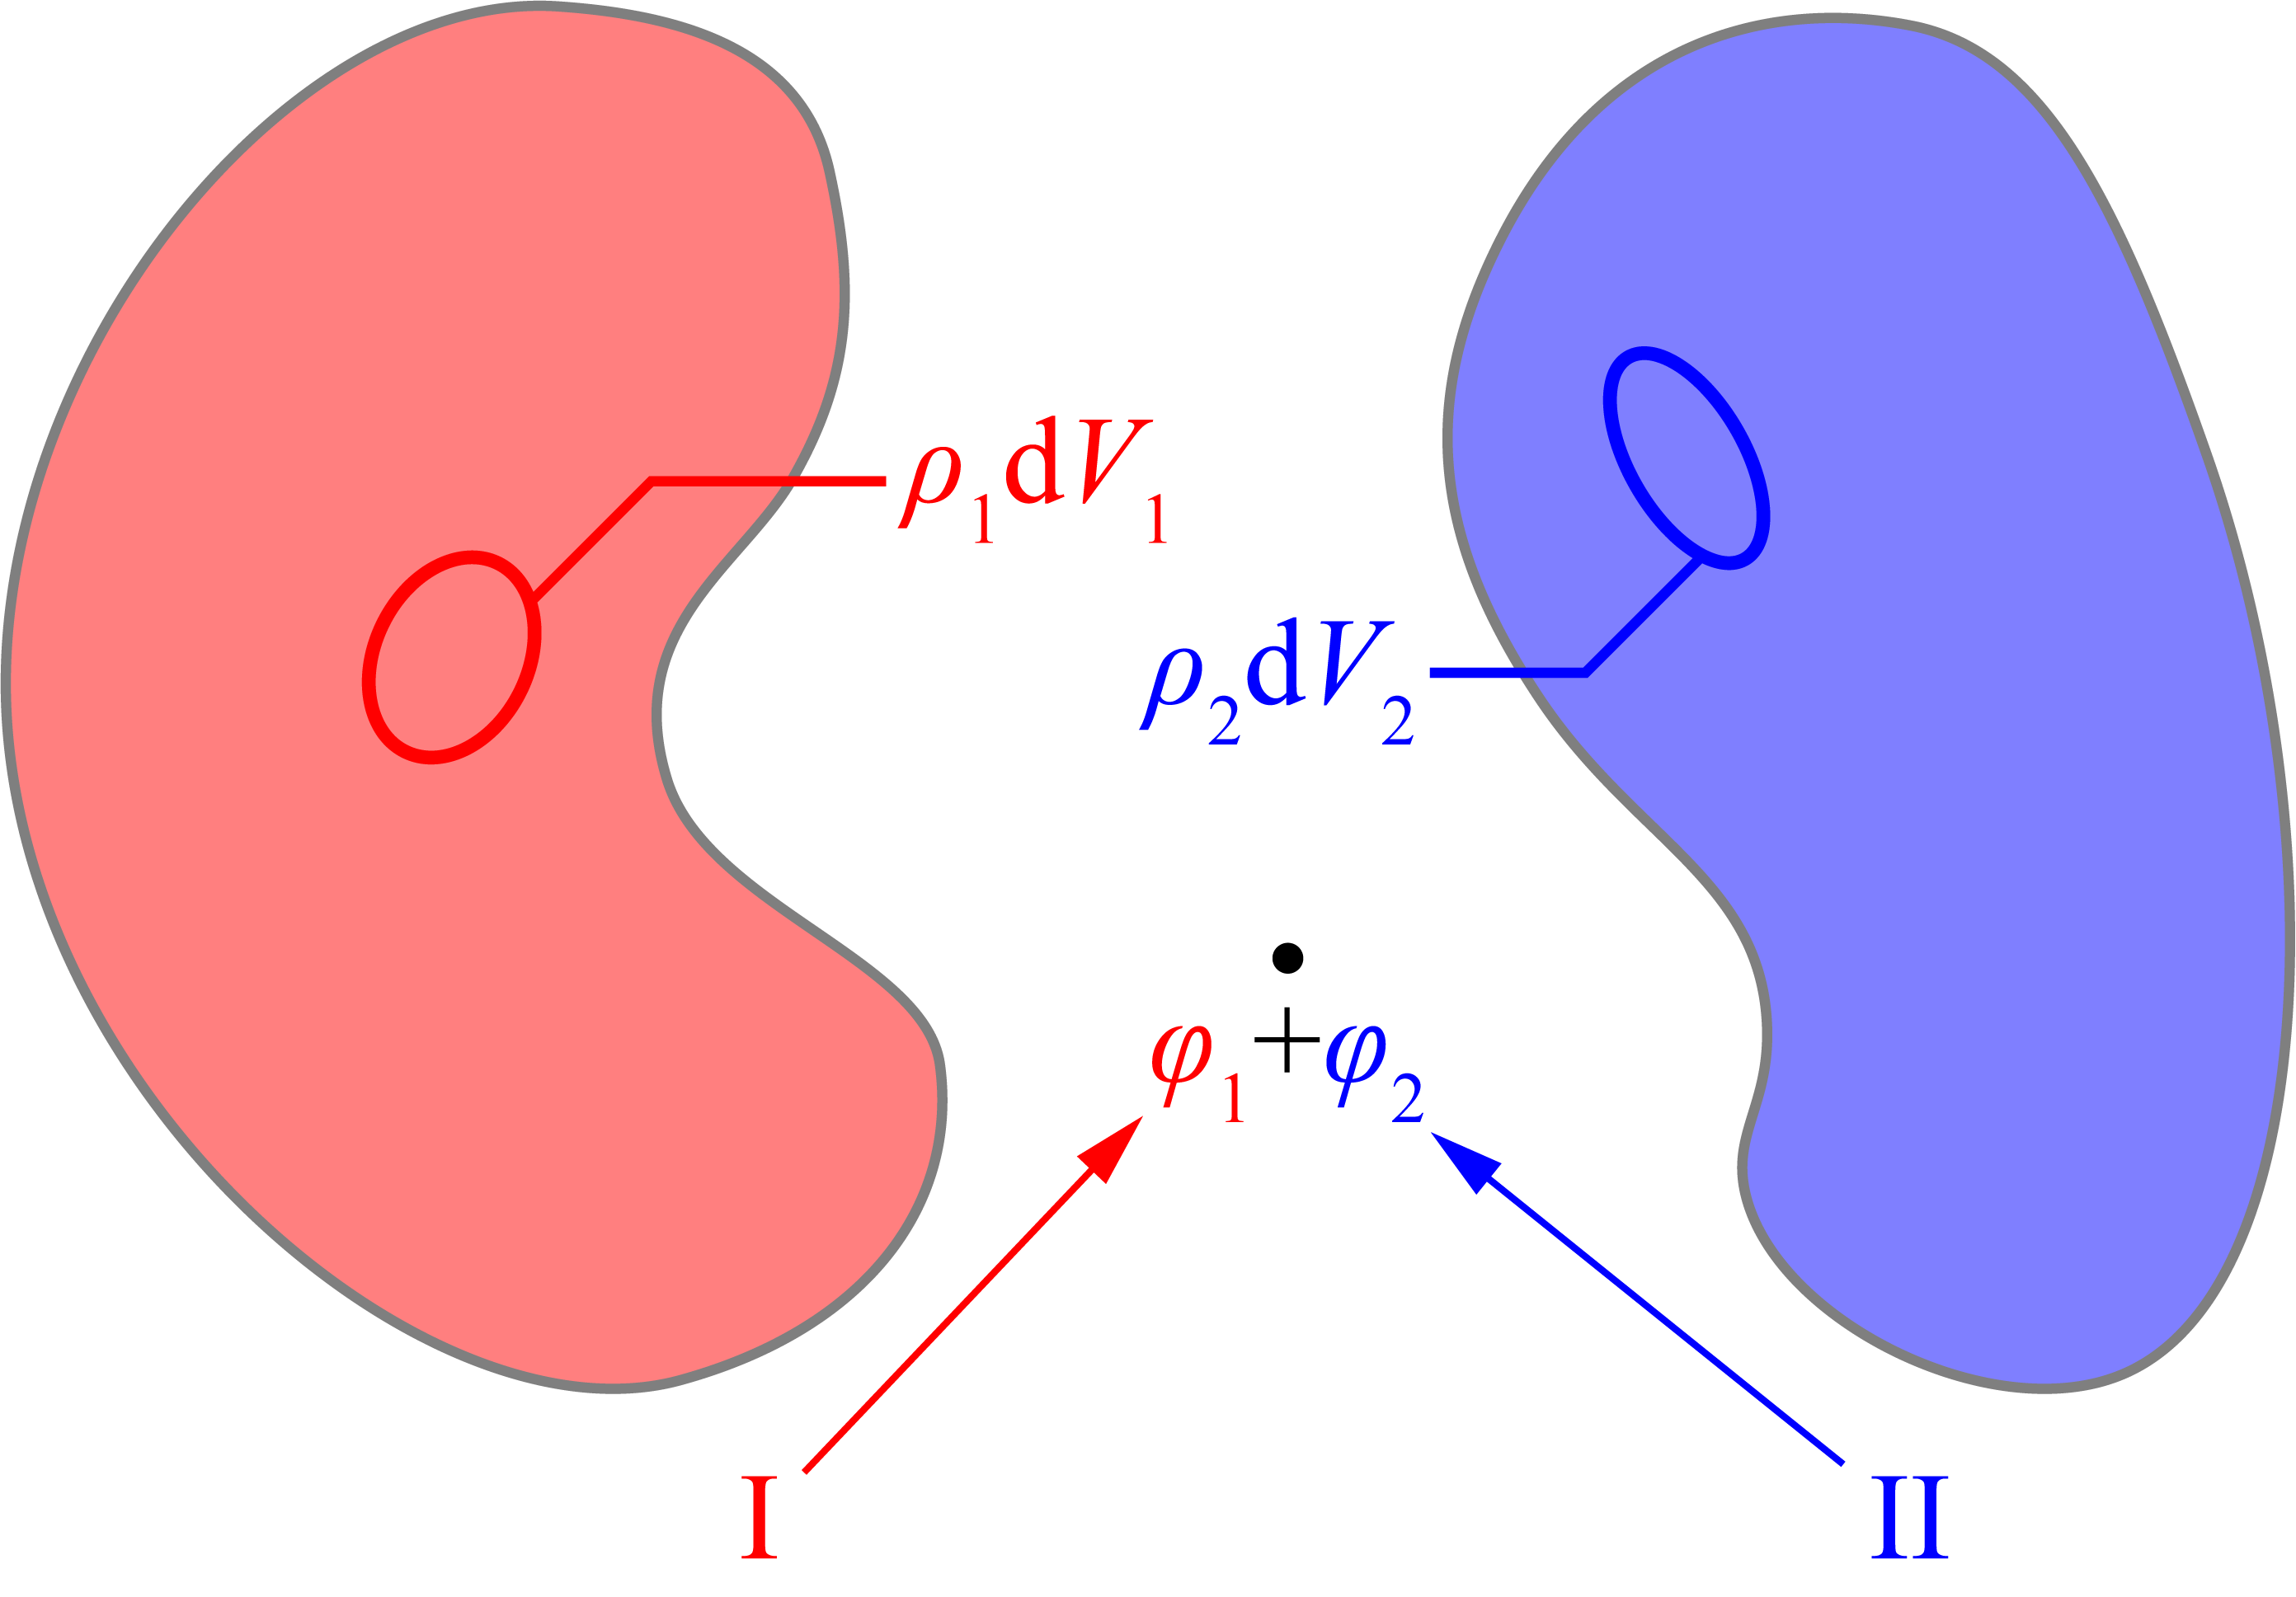
\includegraphics[width=9cm]{image/7-1-9.png}
\caption{自能与相互作用能}
\end{wrapfigure}
我们于是找到了三个能量,\,$I_1,\,I_2$是两个电荷分布体系单独存在时各自的自相互作用能,\,我们把它简称作\emph{自能}(self-energy),\,它一定是大于零的,\,这一点下一节就可以发现.\,而余下的交叉求和项就是表示两个体系之间的相互作用能.\,仔细一看不难发现一项其实就是电荷体系${\rm II}$产生的外场下电荷体系${\rm I}$的电势能,\,而另一项就是电荷体系${\rm I}$产生的外场下电荷体系${\rm II}$的电势能,\,两者仔细研究下发现其实相等:
\[I_{12}=\int\limits_{\rm I}\int\limits_{\rm II}\ke\frac{\rho_1\rho_2}{r}\ud V_1\ud V_2=\int\limits_{\rm I}\rho_1 \varphi_2\ud V_1=\int\limits_{\rm II}\rho_2 \varphi_1\ud V_2\]

这一项可以大于零也可以小于零,\,表示的是相互作用.\,现在我们试探电荷体系在外场中的电势能有了一个新的看法,\,它其实表示试探电荷体系与场源电荷体系的相互作用能,\,作为相互作用,\,它也可以反过来用场源电荷体系在试探电荷体系产生的场中的电势能来计算,\,或是对称地,\,用两者和的一半来计算.

最后让我们来看一下点电荷的自能.\,实际上在之前点电荷体系相互作用能体系中我们已经指出,\,其表达式中电荷$q_i$上电势$\phi_i$与真实电势$\varphi_i$的区别就在于没有计及点电荷在自己位置处产生的电势$\varphi_{ii}$,\,从而漏掉的项其实就是点电荷的自能:
\[I_i=\frac{1}{2}q_i\varphi_{ii}\]

这些项不会影响我们的实际计算,\,因为点电荷总被我们认为是没有内部改变的理想体系,\,我们经常把微观基本粒子做这样的抽象,\,因为它们都是小到可以忽略其尺寸.\,当粒子速度远小于光速,\,且不涉及到高能粒子反应的情况下,\,它们也的确不发生任何内部的改变,\,自能精确地保持不变.\,所以只需要计算扣除点电荷自能的相互作用能表达式,\,就能够知道有多少势能被存储在场中,\,就能够用它来写出电荷分布发生改变时释放出来的能量.

点电荷的自能如何计算呢?\,这取决于我们采取的模型.\,如果我们考虑的是一个电荷均匀分布在表面的球体,\,那么自能为:
\[I=\frac{1}{2}Q\cdot\ke\frac{Q}{r}\]

对于电子,\,如果我们认为电子的静质量全部来源于它携带的场的惯性,\,那么能够写出:
\[I=\frac{e^2}{8\pi\varepsilon_0 r}=m_e c^2\]

事实上我们并不能确定电子内部电荷分布,\,所以我们更常直接定义\emph{经典电子半径}(classical electron radius)为:
\[\frac{e^2}{4\pi\varepsilon_0 r_e}=m_e c^2\quad \Rightarrow \quad r_e=\ke \frac{e^2}{m_e c^2}=2.82\times 10^{-15} {\rm m}\]

然而这仅仅是一个方便计算的实用常数,\,并不能代表电子的真实情况!\,事实上用不带电荷的粒子与电子发生散射实验就会发现,\,电子的尺寸比这要小得多,\,上面的计算结果甚至比质子的半径还要大几倍!\,而实验更是发现电子在多种意义下就是一个点粒子,\,根本没有内部组成结构,\,十分稳定不能衰变.\,那么显然从上式发现这也面临着自能发散的问题.\,双重矛盾如何解决呢?

解决方案是量子力学的引入,\,电子不是点粒子,\,在原子尺度下电子就已经必须要由波函数描述了,\,电子没有同时确定的位置和速度,\,在原子外形成``电子云''.\,\emph{狄拉克}({\it P. Dirac})于1928年提出\emph{狄拉克方程}(Dirac equation),\,把电子像光子那样处理为一个传播的``场'',\,从而从根本上摒弃了电子作为点电荷的观点,\,电子的质量被理解为场的质量或者静能,\,而电子的电荷量被理解为与电磁场(光子)的耦合常数.\,从而把电荷作为一种物质和场物质彻底分割开来独立描述.\,还同时一并给出了电子的自旋与预言了电子的反物质:\,\emph{正电子}(positron)的存在.\,它们都被天然而巧妙的包含在一个统一的代数形式中,\,极大程度地推动了物理学理论的进展.

但这没有给出问题的全部解释,\,对于点电荷自能发散的问题这种做法仍然没有给出绝对的答案.\,经典地看一个匀速运动的经典无穷小点电荷会携带着一个发散的场共同向前运动,\,这在量子场论语言下,\,变成了电子与光子相互作用的无限可能性求和,\,从而也理所当然地引进了各种各样的发散.\,对于这些发散物理学家们发展出了各种各样的处理方法,\,但直到今天还仅仅停留在现象解释的层面,\,背后是否有更加简单的解释方法还是一个谜.


\subsection{电场能}

我们已经十分熟悉,\,电荷之间的相互作用能实际上就是场的能量.\,我们现在将给出这一说法的定域化描述.\,记得一个电荷连续分布体系的相互作用能为:
\[I=\frac{1}{2}\int\limits_V \rho\varphi\ud V\]

而又根据场与电荷之间的关系:
\[\nabla^2 \varphi=-\frac{\rho}{\varepsilon_0}\]

我们把以上积分写为:
\[I=-\frac{\varepsilon_0}{2}\int\limits_V \varphi\nabla^2\varphi\ud V\]

再根据著名的\footnote{而\emph{第二格林等式}(Green's second identity)在格林函数法解边值问题时将十分有用:
\[\nabla\cdot(\phi\nabla\psi-\psi\nabla\phi)=\phi\nabla^2\psi-\psi\nabla^2\phi\]}\emph{第一格林等式}(Green's first identity):
\[\nabla\cdot(\phi\nabla\psi)=\phi\nabla^2\psi+\nabla\phi\cdot\nabla\psi\]

我们再取$\phi,\,\psi$都为$\varphi$,\,从而:
\[\varphi\nabla^2\varphi=\nabla\cdot(\varphi\nabla\varphi)-(\nabla \varphi)^2\]

带入以上积分,\,我们得到:
\begin{align*}
I 	&=\frac{\varepsilon_0}{2}\int\limits_V (\nabla \varphi)^2\ud V-\frac{\varepsilon_0}{2}\oint\limits_{\partial V} \varphi\nabla\varphi\cdot\ud \bs{A}\\
	&=\int\limits_V \frac{\varepsilon_0}{2} \bs{E}^2 \ud V + \frac{\varepsilon_0}{2}\oint\limits_{\partial V} \varphi\bs{E}\cdot\ud \bs{A}
\end{align*}

我们总是考虑电荷分布有限的情况.\,此时最初的积分体积只要包含所有电荷即可,\,那么我们最后得到的这个恒等式就十分的有意思,\,,它将一个体系的相互作用转化为了一个量的体积分和另一个量在包含所有电荷的面上的面积分的形式.\,我们如果取体积为无穷大的全空间,\,那么考虑到随着远离电荷体系$R$处$\varphi$以至多$\dfrac{1}{R}$的方式衰减(若体系总电荷量为零则衰减更加剧烈),\,而$\bs{E}$以至多$\dfrac{1}{R^2}$的方式衰减,\,而积分面积以$R^2$的方式增加,\,故整个积分以至多$\dfrac{1}{R}$的方式衰减,\,在无穷远处这个积分的第二项就会趋于零.\,

从而我们得到了:
\[I=\int \frac{\varepsilon_0}{2} \bs{E}^2 \ud V\]

从而发现相互作用能可以用场来定域地计算.\,电场的\emph{能量密度}(energy density)为:
\[w_e=\frac{\varepsilon_0}{2} \bs{E}^2\]

场的能量不再由电荷造成,\,而是由场自己的场强去定义,\,以后还会进一步证明,\,场在一点处对电荷有力的作用,\,将会使场的动量密度发生改变,\,而对电荷有做功,\,将会影响这一点处的能量密度.


\section{电荷体系}

讨论若干电荷体系对于之后问题的理解是大有帮助的.\,这些包括:

\subsection{电偶极子}

\begin{wrapfigure}[11]{o}[0pt]{7cm}
\centering
\vspace{-2cm}
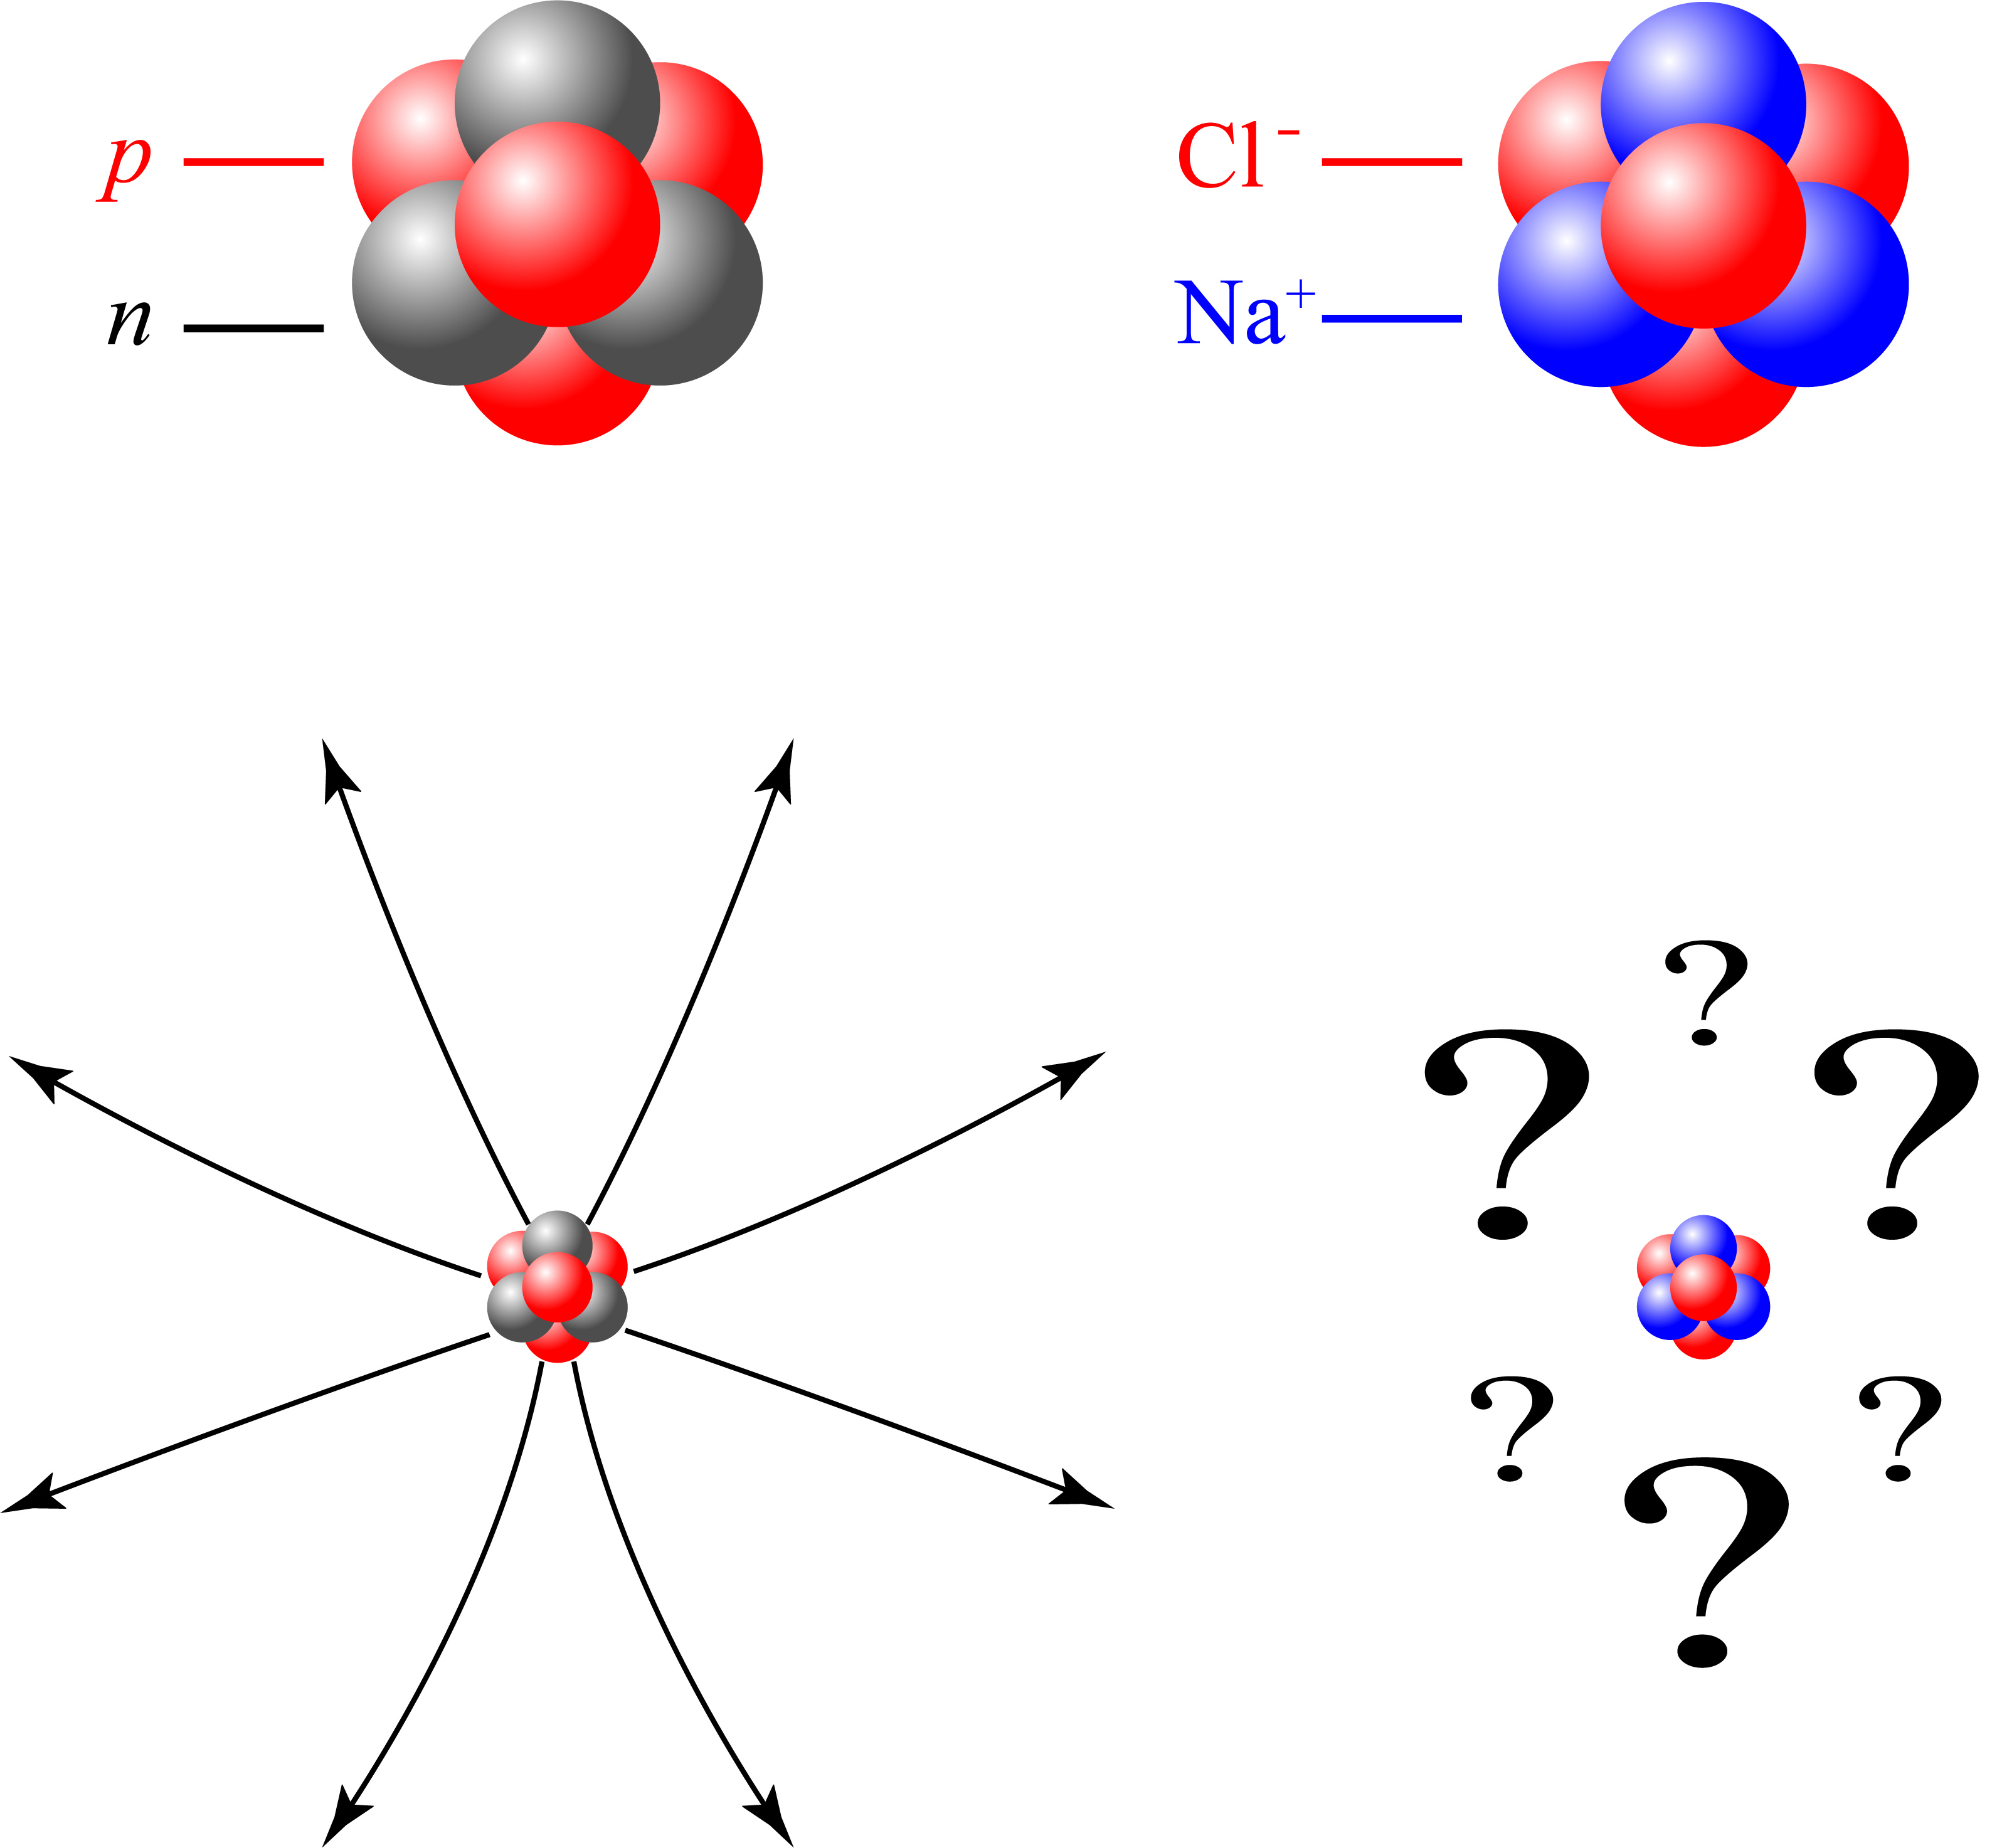
\includegraphics[width=7cm]{image/7-1-10.png}
\caption{远方的场}
\end{wrapfigure}
我们都知道一个电荷体系如果带电,\,那么尽管在离电荷体系很近处电场分布不均匀,\,但离开分布电荷足够远处的场强却总是趋于一个点电荷的电场.\,常见的情况发生在原子核中,\,原子核由质子和中子组成,\,质子带电而中子不带电.\,原子核内电荷分布总是不均匀的,\,但在考虑外界电子受力时总是将其产生的场视为库仑场.\,这是因为电子典型半径:\,玻尔半径与原子核的尺寸比差了$5$个数量级.\,在这个距离处电场完全可以看成是库仑场,\,它与库仑场的偏离将作为一个可以忽略的小量而不去考虑.

但类似的,\,我们将考虑到很多不带净电荷的电荷分布体系,\,它们在近处产生一个不均匀的电场,\,而在远处产生的电场却总是存在着某些规律.\,这个问题有重要的实用价值.\,比如我们如果从${\rm NaCl}$晶体中取出一小块来,\,它的总电量总是为零,\,但由于晶体的变形等因素导致正负电荷产生的电场并不能完全抵消,\,这个电场将会与晶体的动力学耦合,\,极大地影响晶体的动力学特征.\,又比如很多分子实际上属于\emph{极性分子}(polar molecule),\,由于原子的\emph{电负性}(electronegativity)差异,\,原子间的键合具有极性,\,在很多情形下一个原子对公用电子对的吸引能力更强,\,导致电子集中在一个原子一侧.\,从而负电荷的中心向这个原子位移.\,只要分子结构上的对称性不会使得键的极性不会相互抵消,\,整个分子就会显示出极性来,\,它是溶液中溶剂溶解机理的关键,\,也会影响物质的熔点,\,沸点,\,极化率等等关键的物理特性.

\begin{wrapfigure}[11]{o}[0pt]{6cm}
\centering
\vspace{-0.6cm}
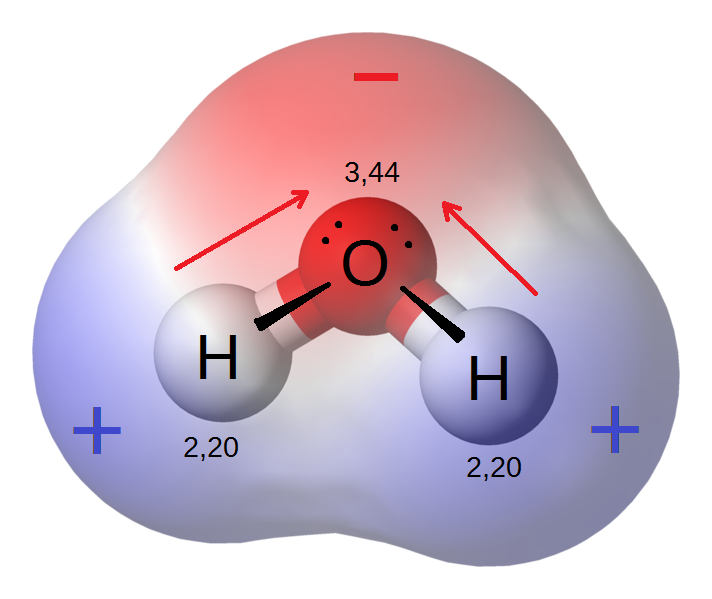
\includegraphics[width=6cm]{image/7-1-11.png}
\caption{水分子极性}
\end{wrapfigure}
所以我们关心总电荷量为零的体系在很远处产生的电场,\,理论上我们可以采取更完整的\emph{多极展开}(multipole expansion)的做法,\,在很多情况下\emph{电偶极项}(dipole term)成为了这种情形下的\emph{领头项}(leading order).\,我们定义小范围分布电荷体系中所有正电荷的``中心''和负电荷的``中心'':
\[\bs{r}_+=\frac{\displaystyle\sum_{q_i>0} q_i \bs{r}_i}{Q}\quad,\quad Q=\sum_{q_i>0} q_i\]
\[\bs{r}_-=\frac{\displaystyle\sum_{q_i<0} q_i \bs{r}_i}{-Q}\quad,\quad -Q=\sum_{q_i<0} q_i\]

而体系的\emph{电偶极矩}(dipole moment)就被定义为由负电荷指向正电荷的矢量:
\[\bs{d}=Q(\bs{r}_+-\bs{r}_-)\]

或者写为:
\[\bs{d}=\sum_{i} q_i \bs{r}_i\]

求和遍及所有电荷,\,无论正负.\,由于总电荷量是零,\,不难验证这个矢量与坐标原点的选取无关,\,为了纪念物理学家\emph{德拜}({\it P. Debye})在分子物理领域的相关开创性工作,\,它一般使用以德拜命名的单位,\,它是一个高斯制单位:
\begin{align*}
1 \;{\rm D} 	&=10^{-18} \;{\rm statC\cdot cm} \\
			&=\frac{1}{299792458}\times 10^{-21} \;{\rm C\cdot m} \\
			&=3.34\pow{-30} \;{\rm C\cdot m} \\
			&=0.208 \;{\rm e\cdot \angstrom}
\end{align*}


\begin{wrapfigure}[8]{o}[0pt]{4cm}
\centering
\vspace{-2.5cm}
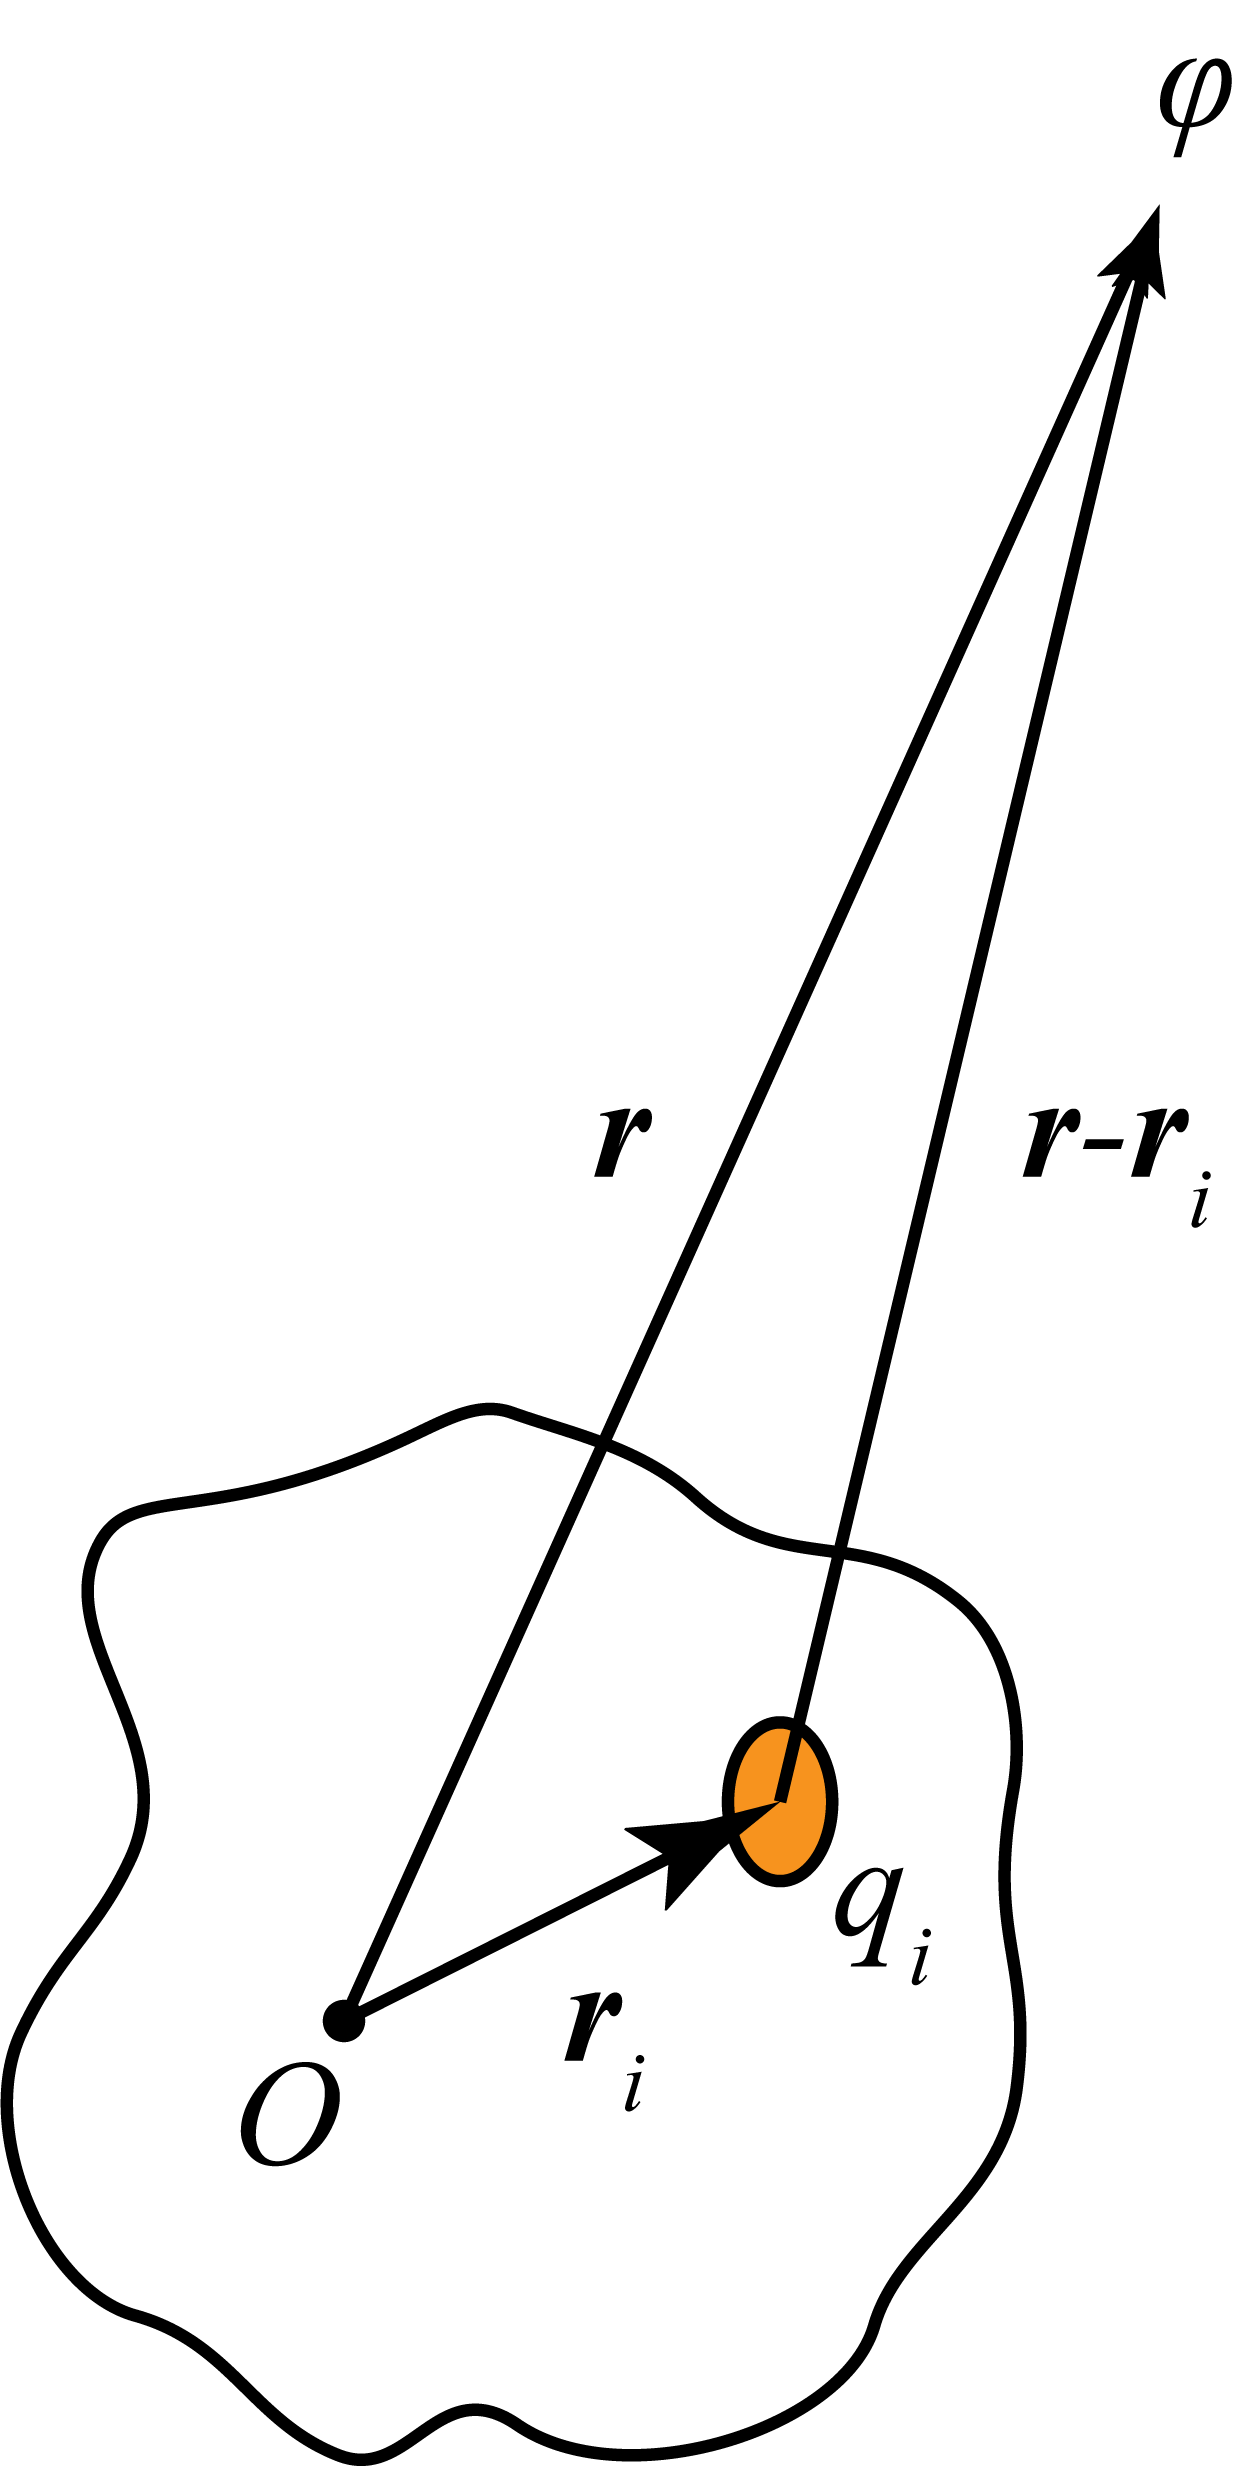
\includegraphics[width=4cm]{image/7-1-12.png}
\caption{偶极展开}
\end{wrapfigure}
为何定义这样的一个矢量呢?\,我们考察在原点附近分布了一个电荷体系$\{q_i ,\, \bs{r}_i\}$,\,那么在很远处产生的电势应该为:
\[\varphi(\bs{r})=\sum_i \ke \frac{q_i}{|\bs{r}-\bs{r}_i|}\]

而对于分母中的矢量的模,\,我们考虑到$|\bs{r}|\gg|\bs{r}_i|$,\,可以做如下近似:
\begin{align*}
\frac{1}{|\bs{r}-\bs{r}_i|} 	&=[(\bs{r}-\bs{r}_i)^2]^{-\frac{1}{2}}=(\bs{r}^2-2\bs{r}_i\cdot\bs{r}+\bs{r}_i^2)^{-\frac{1}{2}} \\
								&\approx (r^2-2\bs{r}_i\cdot\bs{r})^{-\frac{1}{2}}=\frac{1}{r}(1-2\frac{\bs{r}_i\cdot\bs{r}}{r^2})^{-\frac{1}{2}} \\
								&\approx \frac{1}{r}(1+\frac{\bs{r}_i\cdot\bs{r}}{r^2})=\frac{1}{r}+\frac{\bs{r}}{r^3}\cdot \bs{r}_i \\
								&=\frac{1}{r}+\frac{\bs{e}_r}{r^2}\cdot \bs{r}_i
\end{align*}

代入求和表达式,\,得:
\[\varphi(\bs{r})\approx \ke \frac{\displaystyle\sum_i q_i}{r}+\ke \frac{\bs{e}_r\cdot\displaystyle\sum_i q_i \bs{r}_i}{r^2}\]

第一项求和由于总电荷量为零放弃了成为领头项的机会,\,而第二项凸显了出来,\,根据我们之前定义的电偶极矩,\,它实际上就是:
\[\varphi(\bs{r})=\ke \frac{\bs{e}_r\cdot\bs{d}}{r^2} \quad (r\gg d)\]

我们取了等号,\,条件是我们考察的点的矢径$r$远大于电荷分布的平均尺寸$d$.\,而理论上常常构造一种十分独特的体系,\,我们让一对电量为$+Q$与$-Q$严格相等的点电荷相离$\bs{r}_+-\bs{r}_-=\bs{l}$,\,再令$Q\to\infty$而$\bs{l}\to \bs{0}$,\,而保持$\bs{p}=Q\bs{l}$的值保持不变,\,其极限就是抽象的模型:\,\emph{点电偶极子}(point dipole),\,它在除原点外,\,全空间产生的电势都可以用上式来表示.\,这也是我们以后讨论的中心.\,如果在点电偶所在空间点建立球极坐标系,\,而把电偶极矩矢量指向的方向作为极轴,\,我们可以写出电势为:
\[\varphi(r,\,\theta)=\ke\frac{p\cos\theta}{r^2}\]
\begin{wrapfigure}[11]{o}[0pt]{7cm}
\centering
\vspace{-0.5cm}
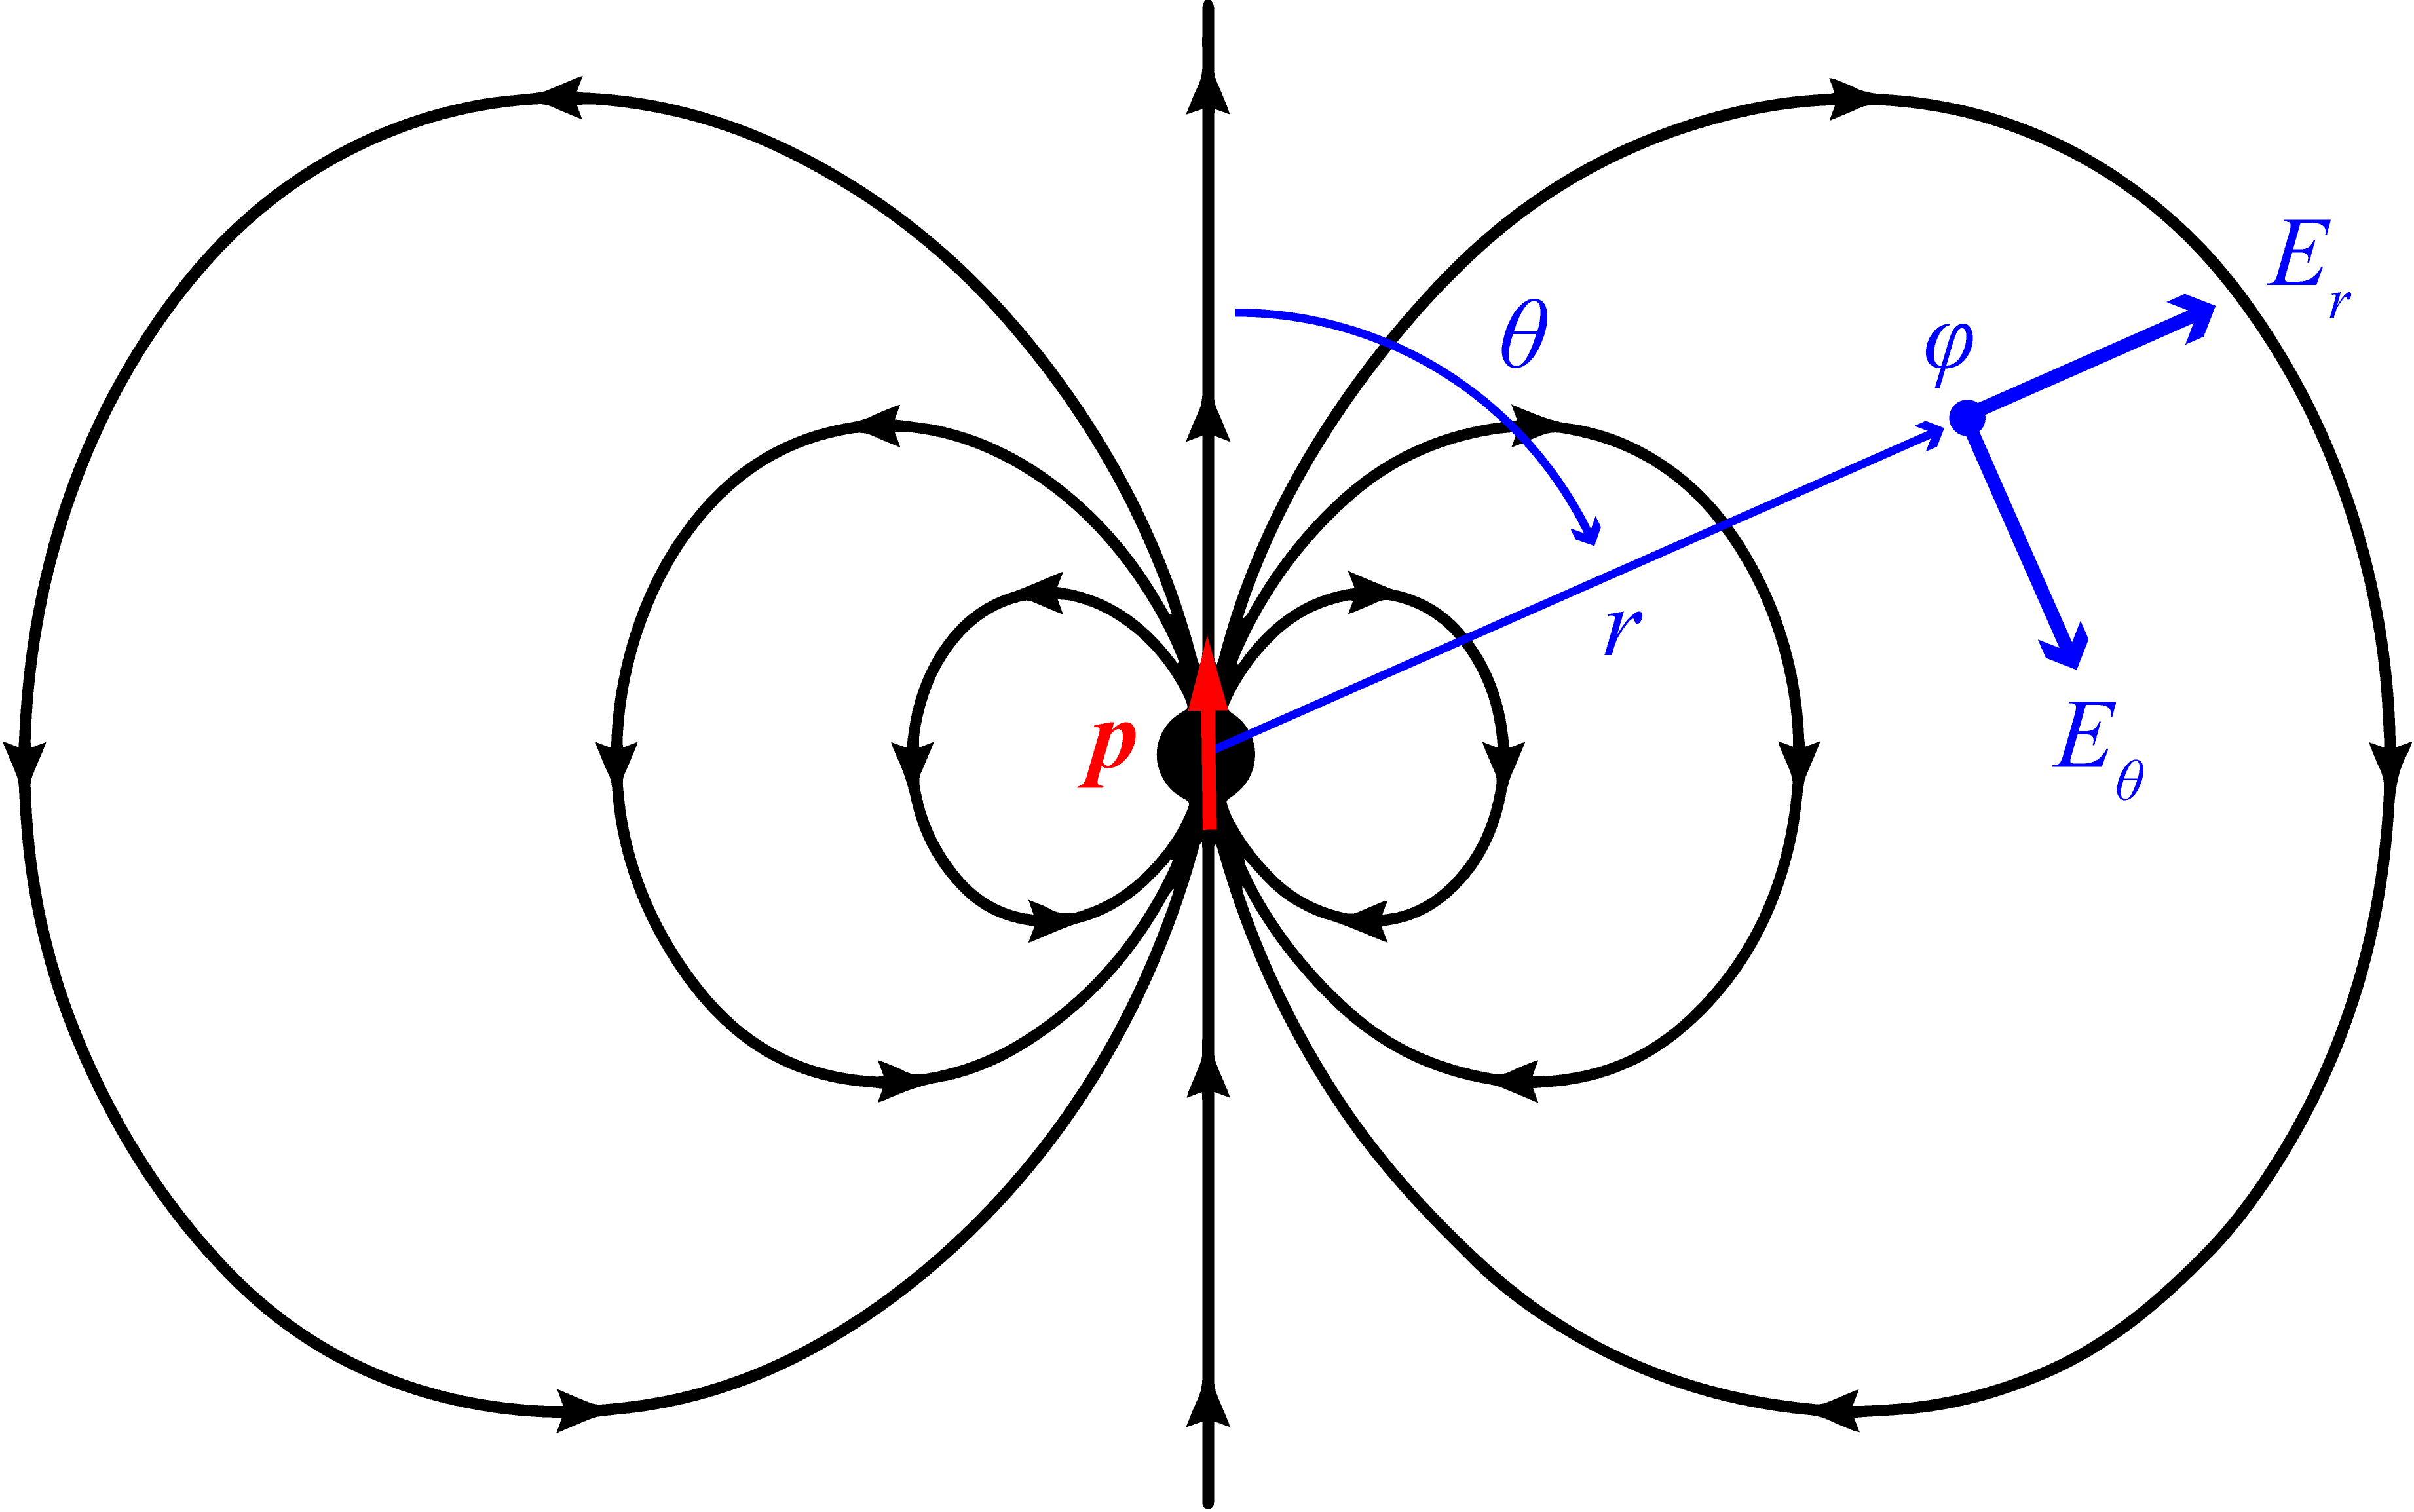
\includegraphics[width=7cm]{image/7-1-13.png}
\caption{点电偶极子的场}
\end{wrapfigure}
这是一个与半径平方反比的电势,\,它与角度有关.\,利用球坐标下梯度算符的表示:
\[\nabla=\bs{e}_r \frac{\partial}{\partial r} +\frac{1}{r}\frac{\partial}{\partial \theta}+\frac{1}{r\sin\theta}\frac{\partial}{\partial \phi}\]

我们计算出点电偶极子的电场来:
\[E_r(r,\,\theta)=\ke\frac{2p\cos\theta}{r^3}\]
\[E_\theta(r,\,\theta)=\ke\frac{p\sin\theta}{r^3}\]

可见电场倒是三次反比了.\,它比点电荷产生的场随距离减少地更快.\,理论研究经常会把以上两个分量式组合为一个矢量式,\,不难验证\footnote{这个表达式对原点以外的点适用,\,如果考虑原点的奇异电场特性,\,并引入\emph{狄拉克德尔塔函数}(Dirac delta function),\,则更准确的表达式为:
\[\bs{E}=\ke \frac{3(\bs{e}_r\cdot\bs{p})\bs{e}_r-\bs{p}}{r^3}-\frac{\bs{p}}{3\varepsilon_0}\delta^3(\bs{0})\]}
\[\bs{E}=\ke \frac{3(\bs{e}_r\cdot\bs{p})\bs{e}_r-\bs{p}}{r^3}\]

如果考虑电偶极子在外场中的情形,\,采用两电荷分布极限为点电偶极子的结果,\,我们很容易发现它的电势能为:
\[V=Q(\varphi_+-\varphi_-)=Q\bs{l}\cdot\nabla\varphi=-\bs{p}\cdot\bs{E}\]

注意到根据电势能的含义,\,这个能量是不包含构成电偶极子的两电荷之间的相互作用能的,\,而在电偶极子在电场中发生位移的过程中我们也应该不能让电偶极子发生结构的改变:\,即,\,$\bs{p}$的大小不能改变,\,但$\bs{p}$的方向,\,位置都可以发生改变,\,随着这两个剩余自由度发生变化,\,电场对电偶极子做的虚功$-\delta V=\delta[\bs{p}\cdot\bs{E}(\bs{r})]$就被理解为力矩与受力:
\[\delta \bs{r}=\bs{0},\;\delta \bs{p}=\delta \bs{\theta}\times \bs{p}:\; -\delta V=\bs{M}\cdot \delta\bs{\theta}\quad \Rightarrow \quad \bs{M}=\bs{p}\times\bs{E}\]
\[\delta \bs{r}\neq\bs{0},\;\delta \bs{p}=0:\; -\delta V=\bs{F}\cdot \delta\bs{r}\quad \Rightarrow \quad \bs{F}=\bs{p}\cdot\nabla\bs{E}\]

其中表达式$\bs{p}\cdot\nabla\bs{E}$的含义为取沿$\bs{p}$方向的矢量场$\bs{E}$的方向导数.\,以后会提到导体或电介质颗粒将会在外电场下感应或极化出一个电偶极子来:
\[\bs{p}=\alpha \bs{E}\]

把此式代入受力公式,\,我们发现:
\[\bs{M}=0\quad;\quad \bs{F}=\frac{\alpha}{2}\nabla{E^2}\]

这也就是我们常说的电场有能够吸引轻小物体的本领的解释,\,我们发现这些小物体在外电场中的受力方向总是指向电场强度大小增加的方向的,\,而与电场强度方向关系不大.

\subsection{电荷密度}

\begin{figure}[H]
\centering
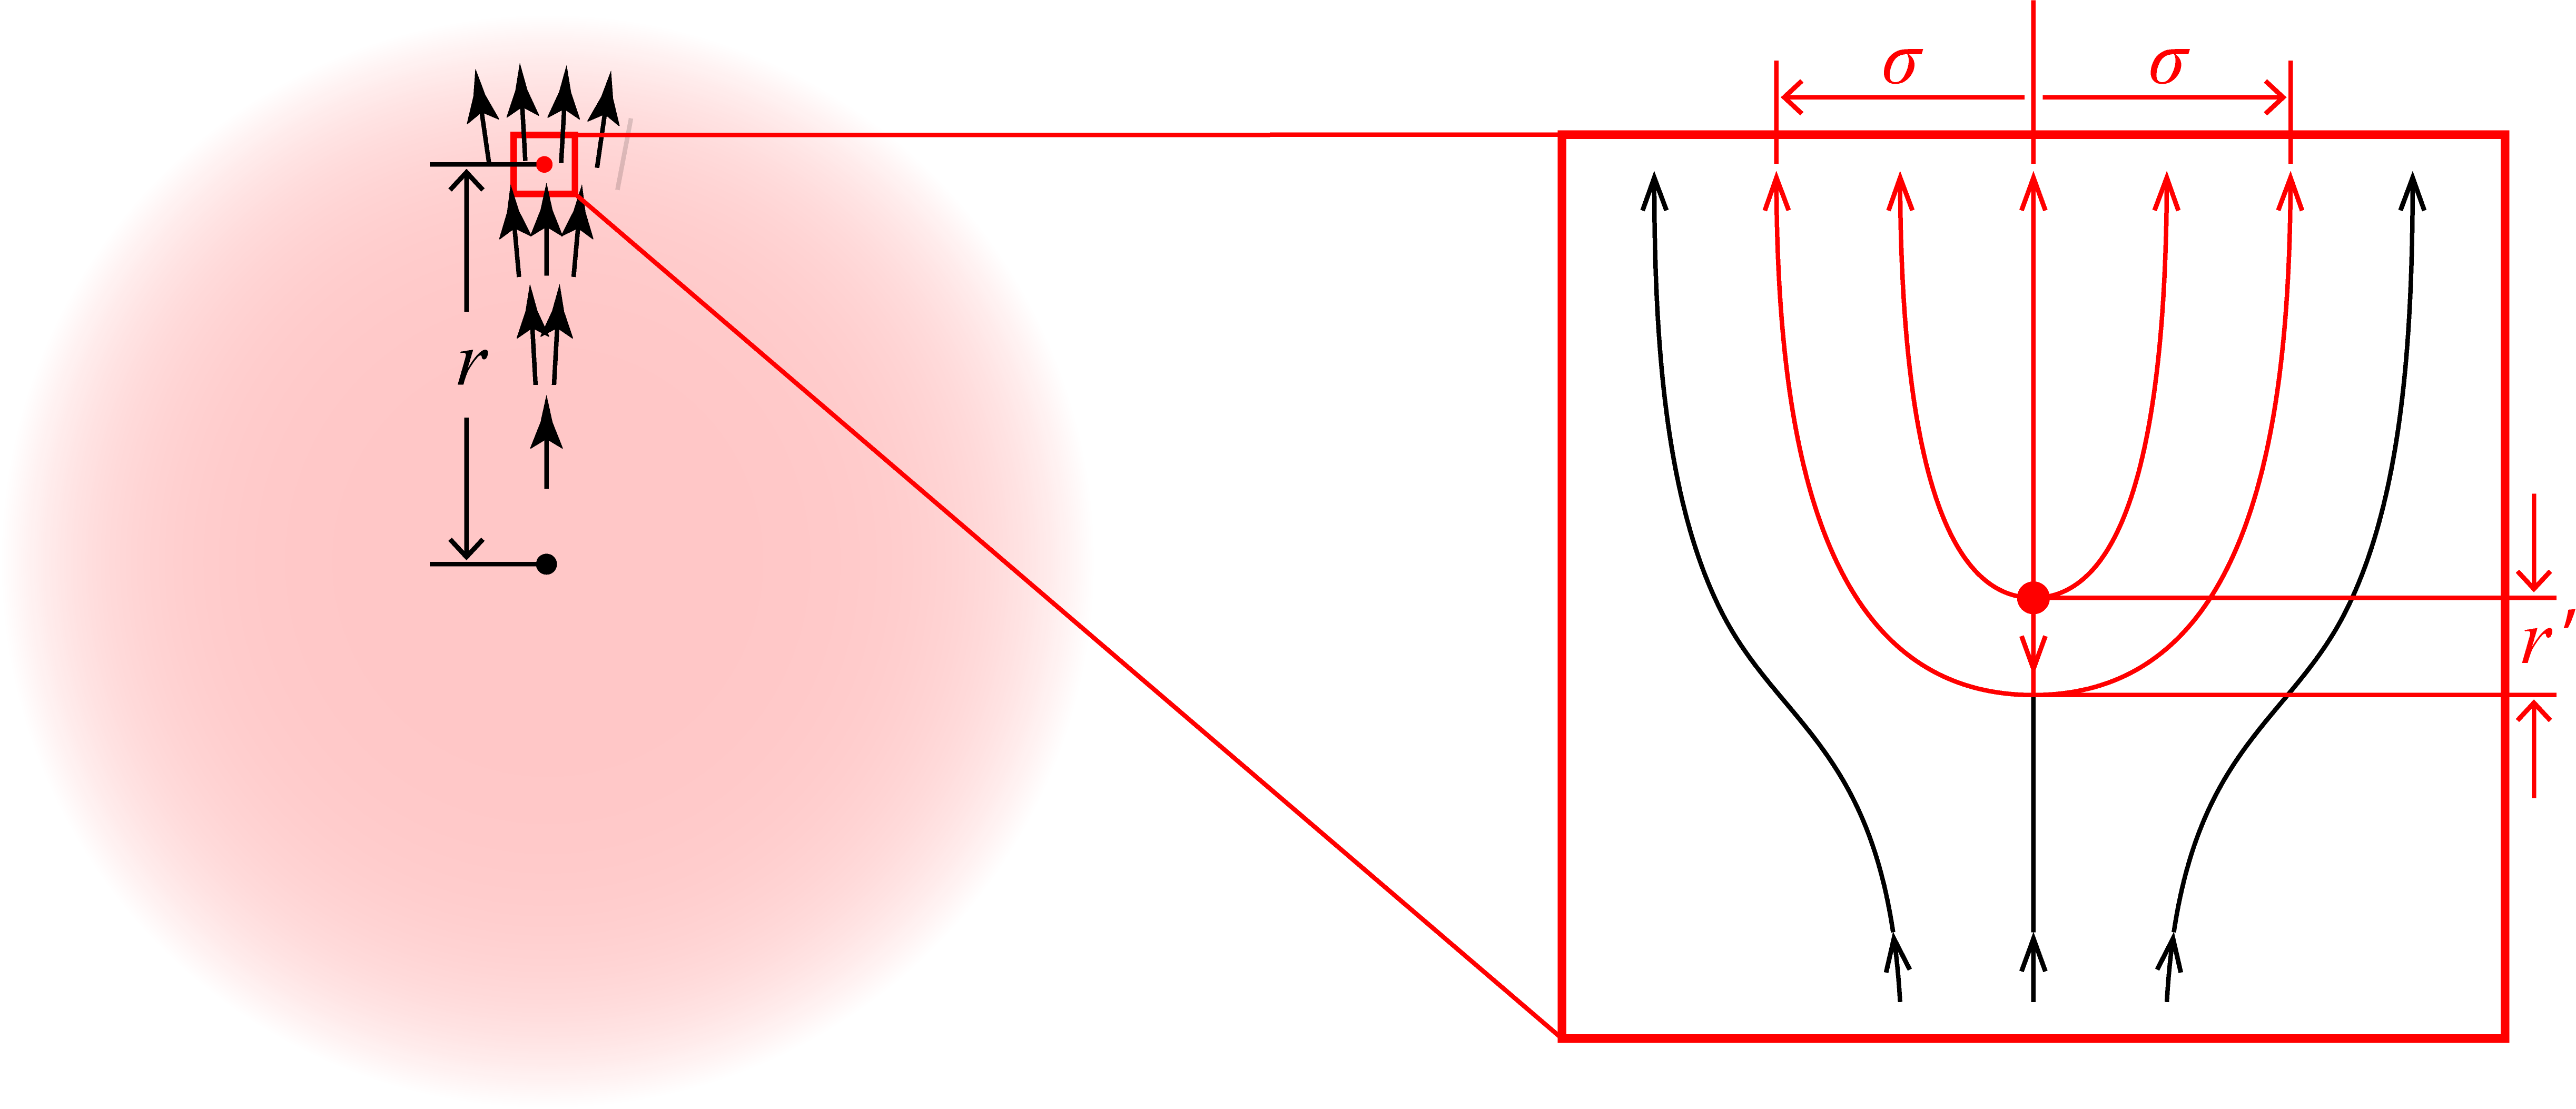
\includegraphics[width=0.5\textwidth]{image/7-1-14.png}
\caption{连续分布点电荷产生平均电场}
\end{figure}
我们经常会用到连续分布的电荷这样的说法,\,把电荷分布写成一个$\rho(\bs{r})$的形式,\,表示每一个体积元$\ud V$中含有的电荷量为$\rho\ud V$.\,这种做法在分析理论问题时发挥了很重要的作用,\,但是它却并不实际.\,实际电荷分布在很小的尺度看来永远是不连续的,\,经典情况下一般可以视为由基本电荷量的点粒子产生的.\,那么正如前述,\,在这样的情况下电荷密度被理解为:
\[\rho=\sum_i n_iq_i\]

更难理解的此时电场强度的定义.\,让我们考虑一个均匀带点的球,\,此时球外的电场强度自然可以简单的按$\dfrac{Q}{4\pi\varepsilon_0 r^2}$来计算.\,若内部的电场若按照完全的连续电荷分布来计算,\,给出了:
\[\bs{E}=\frac{\rho \bs{r}}{3\varepsilon_0}\]

的结果.\,但这个结果忽略了电荷的离散性,\,我们如果认为这个球是由电荷数密度为$n$,\,电荷量为$q$的大量点电荷构成.\,那么设在半径为$r$处的电场与单个点电荷在距中心为$r'$处的电场相等.\,我们可以得到:
\[\frac{nqr}{3\varepsilon_0}=\frac{q}{4\pi\varepsilon_0 r'^2}\]

如果一个电荷的平均占据体积视为球体,\,半径为$R$,\,那么电荷数密度与它的关系为:
\[n\cdot\frac{4}{3}\pi R^3=1\]

这样就得到:
\[\frac{r'}{R}=\sqrt{\frac{R}{r}}\]

或者用$r$区域内包含的电荷数量$N=\left.\dfrac{4}{3}\pi r^3\right/\dfrac{4}{3}\pi R^3$,\,得到:
\[r'=\frac{R}{N^{1/6}}\]

还有一种看法是考察一个电荷发出的电场线在远方形成匀强电场以后的截面:
\[\frac{nqr}{3\varepsilon_0}\cdot \pi\sigma^2=\frac{q}{\varepsilon_0}\]

我们很容易发现:
\[\sigma=2r\]

也就是说,\,离开中心区域越远,\,包含的总电荷数量越多,\,该处点电荷产生的电场相对与由内部大量电荷积累而来的大的几乎均匀的电场相比就足够地小.\,点电荷使得外电场偏离均匀的空间范围就远小于电荷与电荷之间的间距,\,使得电荷之间的空间就可以视为一个几乎均匀的场.

最后我们总结,\,在用堆放点电荷的方式来得到一个电荷密度时,\,尽管微观来看产生的电磁场仍然很不均匀,\,但我们可以抽象出来每一点的平均场强的概念.\,它的意义有二:\,一是下一节即将证明的该点局部微元体积内电场的平均值.\,二是如果保证电荷密度不变电荷无限分散的极限情形下该点处的实际场强.\,它的算法依然是:
\[\bs{E}=\int\limits_{V'} \ke \frac{\rho \bs{e}_{\bs{R}}}{\bs{R}^2} \ud V'\]

而既然电场算法与真实的连续分布的电荷没有区别.\,电势,\,局部电荷受力体密度就仍然可以这样计算:
\[\varphi=\int \ke\frac{\rho}{|\bs{R}|}\ud V'\quad ,\quad \bs{f}=\rho \bs{E}\]

\subsection{极化强度}

往往,\,平常状态下的物质的真实情况是,\,所有局部都不是由单一的点电荷单元堆积而成.\,就比如液体的水,\,它的重复单元是电中性的水分子.\,尽管电中性,\,对外表现出偶极子,\,在原场情况下近似为点电偶极子,\,便是其电势电场的领头项.\,故我们需要考虑的实际情况是:\,单位体积内有$n(\bs{r})$个偶极矩为$\bs{p}(\bs{r})$的点电偶极子.\,这里$\bs{p}$不会是常矢量,\,首先其方向往往随着空间位置逐渐在改变,\,而每个电偶极子的电偶极矩大小亦可能因为极化程度的不同而有所区别,\,下一章我们要介绍的位移极化就是这样的情形.\,我们将数密度$n$与电偶极矩$\bs{p}$相乘,\,得到单位体积内的电偶极矩,\,即\emph{极化强度}(polarization density):
\[\bs{P}=n\bs{p}\]

对于连续情况,\,我们发现电势应该用电偶极子的电势进行体积分来得到:
\[\varphi=\int \ke \frac{\bs{P}\cdot \bs{e}_{\bs{R}}}{\bs{R}^2}\ud V' \quad ,\quad \bs{R}=\bs{r}-\bs{r}'\]

然而我们发现以下等式是成立的:
\[\nabla'=\bs{e}_x\frac{\partial}{\partial x'}+\bs{e}_y\frac{\partial}{\partial y'}+\bs{e}_z\frac{\partial}{\partial z'}\]
\[\nabla'\cdot\frac{\bs{P}}{|\bs{R}|}=\frac{\nabla'\cdot \bs{P}}{|\bs{R}|}+\bs{P}\cdot\nabla'\frac{1}{|\bs{R}|}\]
\[\nabla\frac{1}{|\bs{R}|}=\nabla\frac{1}{|\bs{r}-\bs{r}'|}=-\frac{\bs{r}-\bs{r}'}{|\bs{r}-\bs{r}'|^3}=-\frac{\bs{e}_{\bs{R}}}{\bs{R}^2}\quad,\quad \nabla'\frac{1}{|\bs{R}|}=\nabla'\frac{1}{|\bs{r}-\bs{r}'|}=-\frac{\bs{r}'-\bs{r}}{|\bs{r}'-\bs{r}|^3}=\frac{\bs{e}_{\bs{R}}}{\bs{R}^2}\]
\[\Rightarrow\quad \frac{\bs{P}\cdot \bs{e}_{\bs{R}}}{\bs{R}^2}=\nabla'\cdot\frac{\bs{P}}{|\bs{R}|}-\frac{\nabla'\cdot \bs{P}}{|\bs{R}|}\]

这样我们就得到在区域$V'$内存在极化矢量$\bs{P}$时在全空间产生的电势的公式:
\begin{align*}
\varphi 	&=\int\limits_{V'}\ke (\nabla'\cdot\frac{\bs{P}}{|\bs{R}|}-\frac{\nabla'\cdot \bs{P}}{|\bs{R}|})\ud V'\\
			&=\oint\limits_{\partial V'} \ke \frac{\bs{P}\cdot\ud \bs{A}'}{|\bs{R}|}+\int\limits_{V'}\ke\frac{-\nabla'\cdot \bs{P} \ud V'}{|\bs{R}|}\\
			&=\oint\limits_{\partial V'} \ke \frac{\sigma_P\ud A'}{|\bs{R}|}+\int\limits_{V'}\ke\frac{\rho_P \ud V'}{|\bs{R}|}
\end{align*}

\begin{figure}[H]
\centering
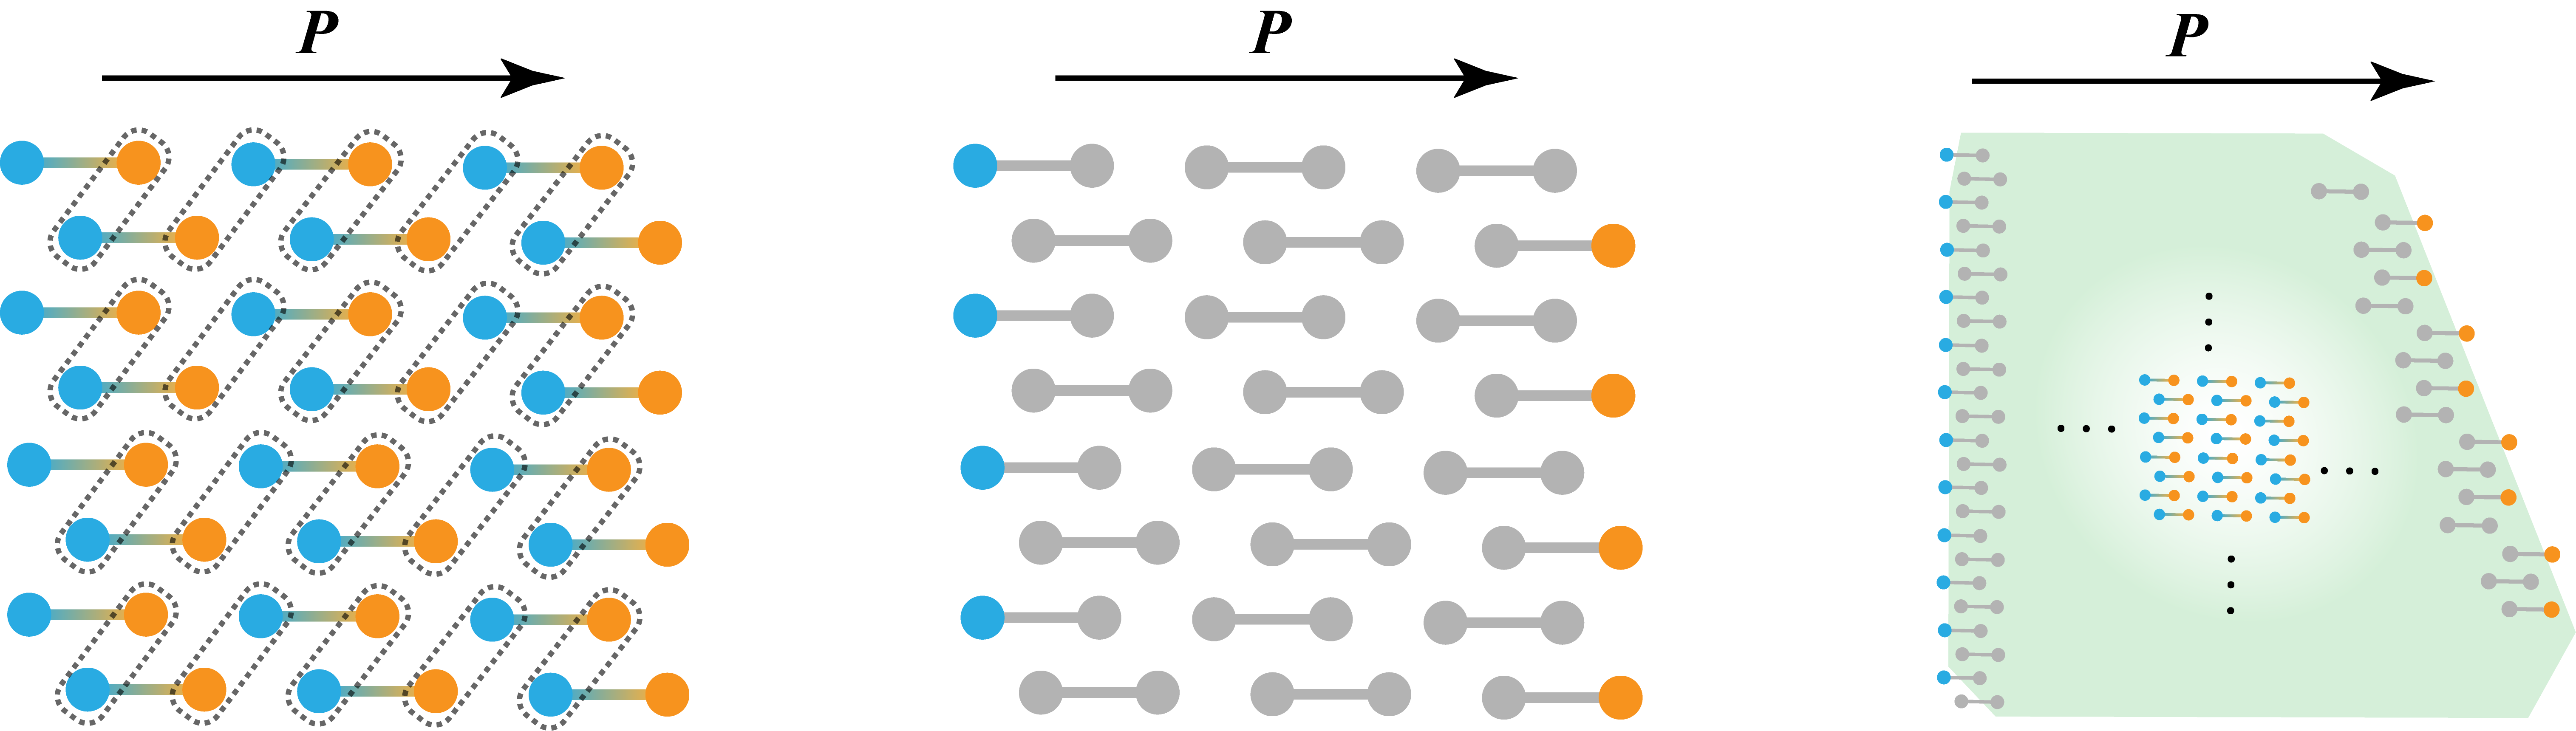
\includegraphics[width=0.9\textwidth]{image/7-1-16.png}
\caption{极化强度导致表面面电荷分布}
\end{figure}

从以上表达式看得出来,\,最后电势有一种等效的求法,\,就是认为在体内有一个$\rho_P=-\nabla'\cdot\bs{P}$的电荷密度分布,\,而认为在体表面的面元$\ud \bs{A}$上带有面电荷$\ud Q=\bs{P}\cdot\ud \bs{A}$,\,或者认为有面电荷密度$\sigma_P=\bs{P}\cdot\bs{n}$,\,其中$\bs{n}$为体积表面的外法向量.\,与其说这是一种等效,\,不如说这只是对实际情况的另一种理解.\,如上图所示,\,这是一块均匀极化的介质,\,我们这样理解介质表面上会出现的电荷:\,对介质内部的电荷进行合适的分组使得一对一对的正负电荷产生的场互相抵消.\,这样便只剩下了表面的电荷能产生场了.\,在几何学上不难证明,\,如果电偶极子长$l$,\,两电荷为$q$,\,体密度为$n$,\,那么在与极化矢量平行的方向看两端未配对电荷的面密度恰好为$\sigma=nql=np=P$.\,再考虑面可能的倾斜便容易发现以上极化电荷面密度$\sigma_P$的公式.\,类似地,\,体电荷密度$\rho_P$对应于沿某方向的$\bs{P}$分量在变化的情形.\,具体的物理图像也请读者加以分析与思考.

我们有把握预期空间各处的电场强度的公式,\,也可以通过上述方式等效,\,毕竟我们可以通过电势计算电场:
\[\bs{E}=\oint\limits_{\partial V'} \ke \frac{\sigma_P\ud A'}{|\bs{R}|^2}\bs{e}_{\bs{R}}+\int\limits_{V'}\ke\frac{\rho_P \ud V'}{|\bs{R}|^2}\bs{e}_{\bs{R}}\]

然而,\,若要开始考虑电偶极子在场中受到的外力,\,那就势必要考虑连续分布的电荷体系产生的电场和微观非均匀分布的电荷体系的局部场之间的区别.\,我们会惊人地发现以上电场只能作为平均意义下的\emph{宏观场}(macroscopic field)而区别于电偶极子具体感受到的\emph{局域场}(local field).\,首先让我们来计算一个概念,\,一个球体内的平均场强$\overline{\bs{E}}$.\,它会计算球体内电荷的受力提供关键线索.\,以原点为中心,\,半径为$R$的球内积分直接得到:
\[\overline{\bs{E}}=\left.\int\limits_{\rm Ball}\bs{E} \ud V\right/ \frac{4}{3}\pi R^3\]

直接计算会具有相当的难度.\,这里采用的技巧是在分子积分中引入$\rho'$常数,\,把积分看做原来的电荷体系产生的电场与均匀分布在这个球体内部的电荷体系之间的相互作用力\footnote{数学上相当于把$1$视作$\bs{r}$的散度的$1/3$,\,即:
\[\nabla\cdot \bs{r}=\frac{\partial x}{\partial x}+\frac{\partial y}{\partial y}+\frac{\partial z}{\partial z}=3\]
}.\,这样的球体产生的电场强度为:
\[\bs{E}'=\begin{cases} \frac{\rho' r}{3\varepsilon_0}\bs{e}_r & (r<R)\\[4pt] \frac{\rho' R^3}{3\varepsilon_0 r^2}\bs{e}_r & (r>R) \end{cases}\]

从而上式被等价写作:
\[\overline{\bs{E}}=\left.\int\limits_{\rm Ball}\rho' \bs{E} \ud V\right/ \frac{4}{3}\pi \rho' R^3=\left.\int\limits_{\rm Ball} \bs{E}\nabla\cdot\bs{E}'  \ud V\right/ \frac{4}{3}\pi \rho' R^3=\left.\int\limits_{\rm all} \bs{E}\nabla\cdot\bs{E}'  \ud V\right/ \frac{4}{3}\pi \rho' R^3\]

最后一步${\rm all}$改为对全空间积分.\,由牛顿第三定律,\,几乎可以肯定上式通过某种化简\footnote{数学上需要用到张量分析,\,过程略去.}后可以得到作用力与反作用力和为零的结论:
\[\int\limits_{\rm all} \bs{E}\nabla\cdot\bs{E}'  \ud V+\int\limits_{\rm all} \bs{E}'\nabla\cdot\bs{E}  \ud V=\bs{0}\]

于是把原电场对应的电荷密度记做$\rho$,\,待求的量变成:
\[\overline{\bs{E}}=-\left.\int\limits_{\rm all}\rho \bs{E}' \ud V\right/ \frac{4}{3}\pi \rho' R^3=\ke\frac{-\int\limits_{\rm Ball}\rho \bs{r}\ud V}{R^3}+\int\limits_{\rm all-Ball}\ke\frac{\rho(-\bs{e}_r)}{r^2}\ud V\]

\begin{figure}[H]
\centering
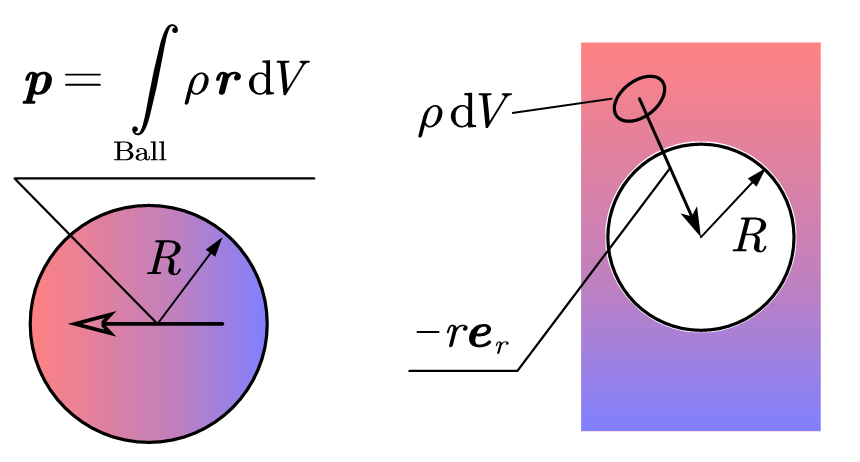
\includegraphics[width=0.6\textwidth]{image/7-1-17.png}
\caption{球内平均电场的两项积分}
\end{figure}

通过以上结果我们发现,\,在一个电荷分布体系中的一个球体内的平均电场取决于两项积分.\,第一项不是别的,\,就是直接取决于球内电荷分布产生的电偶极矩$\bs{p}$.\,第二项则代表外界电荷直接对球心处产生的电场\footnote{这意味着如果球内没有电荷,\,那么对球内电场做平均的结果恰好得到球心处电场.\,这种性质称作\emph{调和}(harmonic).}.

接下来可以进行以下推演:\,如果外界电荷不是那么紧密地靠近球面,\,那么我们可以通过球面把电荷体系分为两部分.\,现在我们来关心内部这些电荷的受力.\,依然从电场考虑,\,由于外部电荷离球面较远,\,故可以近似认为在球内产生一个均匀的电场$\bs{E}_{\rm ex}$,\,甚至于它就可以近似地等于对球心处的场强,\,这样我们就把之前的式子写为:
\[\overline{\bs{E}}=\ke \frac{-\bs{p}}{R^3}+\bs{E}_{\rm ex} \quad\Rightarrow \quad \bs{E}_{\rm ex}=\overline{\bs{E}}+\ke \frac{\bs{p}}{R^3}\]

如果让求平均的体积非常小,\,而电荷又总是连续化,\,那么$\overline{\bs{E}}$又应当与之前通过极化电荷分布计算的体内点场强$\bs{E}$无异.\,我们已经观察到一个十分关键的信息:\,考虑球内电荷受力时应当使用的外界的场$\bs{E}_{\rm ex}$,\,它与忽略电荷不连续性而计算出来的``平均场''$\bs{E}$存在一个差.\,最后考虑到极化强度的定义$\bs{P}=\lim\limits_{R\to 0}\bs{p}\left/\frac{4}{3}\pi R^3\right.$,\,最终我们得到:
\[\bs{E}_{\rm ex}=\bs{E}+\frac{\bs{P}}{3\varepsilon_0}\]

这个细节对理解介质的极化十分重要.\,我们将会在下一章重新回到这个问题.

\subsection{若干对称带电体系的场}

%!TEX root = ../physical-olympics-2.tex
\chapter{导体与介质}




\section{导体与静电平衡}

\subsection{绝缘体与导体}



微观地看,\,物质由原子或分子等组成,\,其中导电现象通常发生在不同情况下:

	\vspace{0.3cm}1. 真空导电:\,一般不会说真空具有\emph{导电性}(conductive),\,因为真空中是没有\emph{载流子}(charge carrier)的\footnote{量子场论认为真空存在电子对的产生湮灭涨落从而具有一定的导电性.}.\,的确,\,在\emph{阴极射线管}(cathode ray tube)中,\,加热一个阴极,\,并辅以合适的偏置电压可以造成真空中的电流.\,或是用一束能量足够的光子去轰击金属表面造成电子逸出,\,甚至纯粹由于阴极表面尖处十分强的电场导致电子直接克服逸出功发射出来.\,三种现象分别称为\emph{热发射}(thermionic emission),\,\emph{光电效应}(photoelectric effect)与\emph{场发射}(field emission).这种电荷的定向移动现象被统一地称为\emph{输运现象}(transport phenomenon).\,由于真空输运的独特性质,\,比如电子不会受到散射,\,平均自由程远大于仪器尺寸,\,与凝聚态物理中的一些概念对应,\,这被称为\emph{弹道输运}(ballistic transport).

	\begin{wrapfigure}[16]{o}[0pt]{5cm}
	\vspace{-1.6cm}
	\centering
	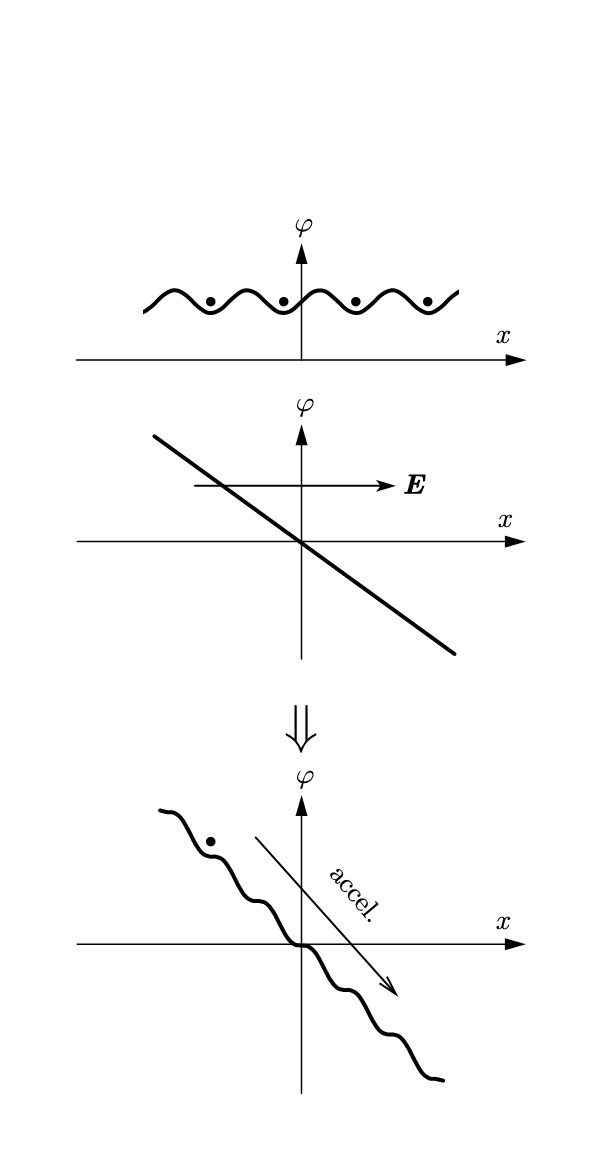
\includegraphics[width=5cm]{image/7-2-1.png}
	\caption{晶体击穿}
	\end{wrapfigure}

	\vspace{0.3cm}2. 绝缘体漏电:\,大多数非金属晶体,\,或是不含离子的液体与气体,\,原子核在晶体中都限制在点阵格子的特定位置,\,在气体,\,液体中则是可以活动的原子分子周围.\,电子分为两类,\,,一类是原子的内层电子,\,它极为稳定地存在于原子周围,\,离子晶体中的几乎完全被阴离子夺取的电子也属于这种情况.\,它们与原子核一起构成\emph{原子实}(atomic core).\,而\emph{价层电子}(valence shell electron),\,它们用来成键,\,将原子连接形成分子或者晶体,\,一般被定域在原子间的特定区域.\,所有这些电子的特点都是\emph{束缚态}(bond state).\,它们不能在介质中自由传导,\,一个电子的区域到另一个电子的区域间存在\emph{势垒}(potential barrirer),\,经典物理认为电子的动能不足以穿过这些势垒.\,但是,\,量子理论则认为电子的波函数可以通过\emph{隧道效应}(tunnelling)以小概率在不同区域间转移.\,这就为有电场的情况下电荷的平均定向移动提供了可能.\,这种现象称为\emph{漏电}(leakage).

	\vspace{0.3cm} 3. 绝缘体击穿:\,在十分高的电场下,\,原子与原子间,\,或是分子中显不同电性的部分之间的典型电压将大于阻碍电子转移的势垒.\,在晶体被击穿时此时电子在本质上可以被视为在周期性势能场与线性势能场的叠加中运动的经典粒子.\,不难看出电子不仅可以脱离单个势阱的束缚,\,还可以在这样的电场力下做持续的加速运动.\,气体液体则是在电场力作用下原子,\,分子被撕裂为离子而继续在电场力下做加速运动.\,此时碰撞就发生了:\,碰撞的结果往往是使得更多的原子分子发生电离.\,这样就会雪崩式的累积,\,固液气中的这些现象都称作\emph{雪崩击穿}(avalanche breakdown).\,尤其是气体中的放电现象在不同电流条件下分别造成\emph{汤森放电}(Townsend discharge),\,\emph{电晕放电}(corona discharge),\,\emph{辉光放电}(glow discharge),\,\emph{电弧放电}(arc discharge)的不同情况.

	\vspace{0.3cm} 4. 自然的导体:\,我们将材料区分为\emph{绝缘体}(insulator)与\emph{导体}(conductor),\,最重要的依据就是在弱场下是否天然地具有能产生电荷输运的载流子.\,所以导体就是一类事先就具有一定数密度$n$的一种或多种载流子$q$的材料,\,它们往往在有电场$\bs{E}$在场时发生位移,\,且与散射造成的形式阻力平衡,\,造成平均的匀速运动,\,即\emph{定向漂移}(directional drift).\,常见的金属以最外层的自由电子为载流子,\,半导体以热激发或掺杂形成的电子或空穴为载流子,\,电解质溶液或部分气态或液态的等离子体以阴阳离子为载流子.\,它们都是典型的导体.\,区别于前三种情况与最后的超导体.

	\vspace{0.3cm} 5. 超导体:\,低温下的很多奇异的宏观现象大大拓宽了人们对量子理论在物理学各个层次中应用的认识.\,其中很典型的一个就是\emph{超导}(superconductivity)现象.\,最早在1911年由\emph{昂内斯}({\it H. K. Onnes})在研究低温下汞的电阻率时惊人的发现在$4.2{\rm K}$下电阻率消失至零,\,这就是超导的发现.\,但是直到约十年后才引起足够重视.\,在$1933$年\emph{迈斯纳}({\it F. W. Meissner})才发现超导不仅仅是电阻率的消失,\,还伴随着\emph{完全抗磁性}(perfect diamagnetism):\,就好像理想导体内部无电场线,\,在超导体中交变的磁场也只能存在于表面极小的深度内(趋肤深度),\,也称\emph{迈斯纳效应}(Meissner effect).\,后来通过量子理论的蓬勃发展,\,在$1957$年提出的\emph{BCS理论}(Bardeen-Cooper-Schrieffer theory)终于解释了超导的成因,\,原来是一对\emph{库珀电子对}(Cooper pair)通过与声子(晶格振动)相互作用而造成了没有任何散射的量子模式.\,完整地解释了直到1986年所有\emph{低温超导}(low-temperatre superconductivity)的现象.\,但是随着$35{\rm K}$超导的镧钡铜氧体的发现,\,宣告人类进入\emph{高温超导}(high-temperatre superconductivity)纪元.\,新的超导材料不断被发现,\,新的理论也不断被提出,\,目前最``高温''的材料是汞钡钙铜氧体,\,超导临界温度$135{\rm K}$.\,为什么有高温超导?\,高温超导的临界温度如何进一步提高?\,直到今天这也还是方兴未艾的研究领域.\,其在科研,\,科技,\,生产,\,生活方面的应用是不可估量的.

\vspace{0.5cm}

我们将把研究的范围主要放在导电的导体和不导电的绝缘体上.\,前者分析其静电平衡,\,即本章要集中讲的情形;\,下一章的稳恒电流和之后章节的拟稳的一些情况则是导体研究的其他场合.\,对于绝缘体我们本章也介绍其介电特性,\,光作为电磁波在介质中的传播则本章做一个抛砖引玉,\,主要内容在光学色散理论中讲解.

\subsection{导体的特点}

这里说的导体,\,主要指固体形式的金属.

首先界定我们研究的问题范围:\,\emph{静电平衡}(electrostatic equilibrium)问题是一种\emph{稳态}(steady state).\,我们研究的问题由各式各样的,\,有限的块状导体${\rm C}_1,\,{\rm C}_2\cdots {\rm C}_n$构成,\,这些导体带电情况由体电荷密度$\rho$和面电荷密度$\sigma$描述.\,但是导体${\rm C}_i$上的总电荷量不一定为零:
\[Q_i=\int\limits_{{\rm C}_i}\rho \ud V+\int\limits_{\partial{\rm C}_i}\sigma \ud S\neq 0\]

这个电量$Q_i$一般也是可以在一定范围内人为控制的,\,即给导体\emph{充电}(charge).\,利用电容的性质很容易可以做到这一点.\,在为导体充电后由于电量守恒,\,其总电量就不能改变了,\,但是其电荷分布一般是未知的.


除了它们往往还有人为指定的各种点电荷$q_j$或者电荷分布$\rho(\bs{r})$存在于导体外.\,那么,\,容易想像,\,当导体外突然产生电荷分布时(如原来中和的电荷被重新分开),\,或者导体被置入电荷体系中,\,本质上就是当导体外的场环境发生改变时,\,导体内部显然不可能保持电场强度始终为零.\,只要有电场就会引起电流,\,它必然使得内部和表面的电荷分布发生改变$\dot{\rho}(t),\,\dot{\sigma}(t)\neq 0$.\,这些状态就是\emph{暂态}(transient state).\,但是只要外界的场不再变动,\,经过特征的\emph{弛豫时间}(relaxation time)后,\,一般很短只有$10^{-14}{\rm s}$量级,\,就会接近,\,直到变成稳态.

通过以上推理,\,足以看出,\,\emph{静电平衡下,\,导体内部应当没有电场.}\,这就是静电平衡理论的初始命题.\,它的初步推演泛化出以下的九宫格式的结论,\,分别讨论导体内,\,导体表面,\,导体外三处的电荷分布,\,电场分布,\,和电势分布三个特性:

\begin{table}[H]
\centering
\begin{tabular}{|c||c|c|c|}
\hline
一般特征	&电荷		  		&电场&电势\\
\hline\hline
导体内 		&$\rho = 0$			&$\bs{E} = 0$	&$\varphi=C$\\
\hline
导体表面	&$\sigma\neq 0$ 	&奇异			&$\varphi=C$\\
\hline
导体外 		&$\rho \neq 0$ 	&$\bs{E} \neq 0$&$\varphi\neq C$\\
\hline
\end{tabular}
\caption{静电平衡的初级结论}
\end{table}

其实就是说,\,因为导体内部没有电场,\,所以导体内部也没有形成电场的电荷(高斯定理可证),\,也使得导体成为一个\emph{等势体}(equipotential body),\,导体表面成为一个\emph{等势面}(equipotential surface).\,注意,\,这里说的``内部'',\,``表面'',\,``外部''包含两种情况.\,导体内部就是金属成分的空间,\,外部一般是真空与外加电荷分布的空间,\,表面是它们的分界面,\,但是下图左的情况,\,导体的外部延伸到了无穷远,\,这种为\emph{开外界}(open exterior),\,但是中和右两种情况,\,导体的外部是有限的\emph{闭外界}(closed exterior).\,第二种典型情况这个单连通的闭外界还被称作\emph{空腔}(cavity).\,除非特殊说明,\,我们一般默认导体的内部不会延伸到无穷远(总是闭的).

\begin{figure}[H]
\centering
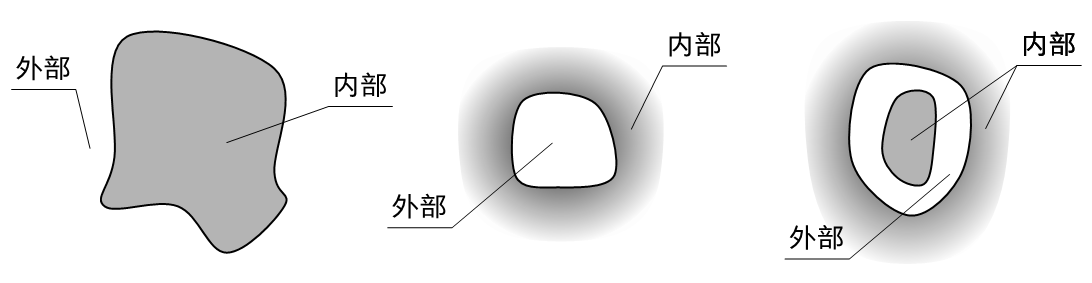
\includegraphics[width=0.7\textwidth]{image/7-2-2.png}
\caption{导体内外}
\end{figure}

在导体表面发生了电场计算的奇异性,\,因为这里是面电荷分布.\,我们考察细节就会进一步发现以下进一步的结论:\,\emph{导体表面的面电荷只朝外侧发出(或吸收)电场线,\,其方向垂直于表面(电场线垂直于等势面),\,且疏密程度正比于电荷密度(即高斯定理).}\,即:
\[\bs{E}=-\nabla\varphi=\frac{\sigma}{\varepsilon_0}\bs{n}\]

\begin{figure}[H]
\centering
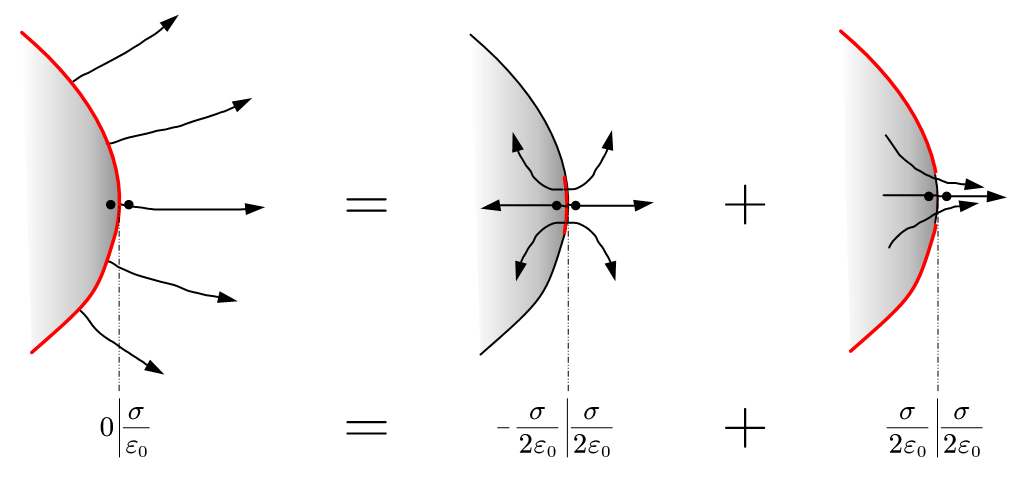
\includegraphics[width=0.6\textwidth]{image/7-2-3.png}
\caption{导体表面}
\end{figure}

但是正如上图所示,\,如果在十分接近表面的内外各取一点,\,就会发现如果只选取相对这两点足够大的一块面电荷(但又足够小以至于可以视作平面),\,它对面左右的电场强度只贡献以上值的一半.\,那么另一半必然由去掉这一块电荷的另外的部分所贡献.\,所以如果要讨论面上的场强,\,通过上一节的球体平均的理解方式,\,它就自然地被定义为内外场强和的一半,\,即:
\[\bs{E}=\frac{\sigma}{2\varepsilon_0}\bs{n}\]

对于导体静电平衡问题的计算求解,\,也包括模拟求解,\,本质上都建立在以下基本原理的基础上:

\begin{verse}
\emph{独立叠加原理}:\,静电平衡问题可以拆解为独立的在导体外部一个个连通区域内的静电边值问题.
\end{verse}

所谓的\emph{边值问题}(boundary value problem)本是偏微分方程的术语,\,在这里特指下面说的静电情况.\,每一种情况中,\,我们无需分析导体的内部的电荷,\,电场,\,电势.\,只需要求解外部的电场$\bs{E}(\bs{r})$和电势$\varphi(\bs{r})$.\,导体外部的电荷分布$\rho(\bs{r})$却是事先给定的.\,还给定了每一种导体表面的,\,要么是电势$V_i$(从而导体内部的电势也是这个值),\,把这种导体称作第一类导体,\,对应条件称为第一类边界条件;\,要么是给定了这个面上的总电量$Q_i$,\,把这种导体称作第二类导体,\,对应条件称为第二类边界条件.\,而每一个导体外部的区域的边界,\,就回到了各个导体的表面$\Sigma_1,\,\Sigma_2\cdots\Sigma_n,\,\Pi_1,\,\Pi_2\cdots\Pi_m$构成的集合.\,但是表面上的电荷分布也是事先不知道的.\,由于电荷,\,电场都可以从电势中得到,\,故只暂时考虑求电势,\,我们把静电边值问题整理一下:

\begin{verse}
\emph{已知}:\,导体外连通区域$D$以第一类导体表面$\Sigma_1,\,\Sigma_2\cdots\Sigma_n$和第二类导体表面$\Pi_1,\,\Pi_2\cdots\Pi_m$为边界.\,已知区域$D$内电荷分布$\rho$,\,已知第一类导体表面$\Sigma_i$上的电势$V_i$.\,已知第二类导体表面$\Pi_j$上的电量$Q_j$:
\[\partial D=\biggl(\bigcup_i \Sigma_i\biggr)\cup \biggl(\bigcup_j\Pi_j  \biggr) \]
\[\rho=\rho(\bs{r}) \quad,\quad \bs{r}\in D\]
\[\varphi(\bs{r})|_{\Sigma_i}=V_i \quad, \quad \int\limits_{\Pi_j}\nabla\varphi\cdot \ud \bs{S}=Q_j/\varepsilon_0 \quad, \quad \varphi(\bs{r})|_{\Pi_j}=C\]

\emph{未知}:\,导体表面电荷的具体分布$\sigma(\bs{r})|_{\Sigma_i,\,\Pi_j}$

\emph{待求}:\,$D$内的电势分布$\varphi(\bs{r})|_{D}$

\end{verse}


\begin{wrapfigure}[19]{o}[0pt]{7cm}
\vspace{-0.6cm}
\centering
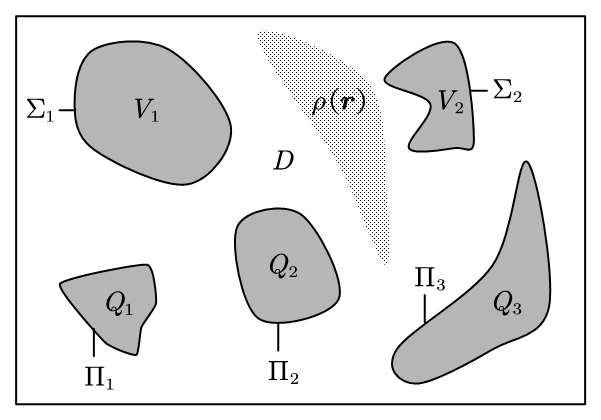
\includegraphics[width=7cm]{image/7-2-4.png}
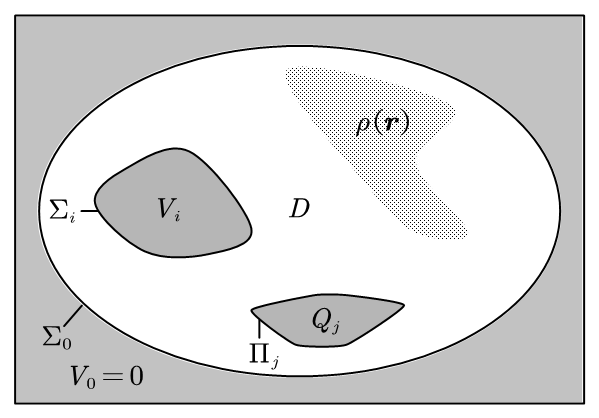
\includegraphics[width=7cm]{image/7-2-5.png}
\caption{边值问题}
\end{wrapfigure}
但是还要注意这种边值问题又分为\emph{外问题}(outside problem)和\emph{内问题}(inside problem)两类.\,外问题是区域$D$延伸到了无穷远,\,这种情况的边值问题提法就完全如上所述.\,但是内问题中区域$D$存在一个最外的表面$\Sigma_0$,\,它把整个$D$和其他所有金属表面与内部包含在其内部.\,$\Sigma_0$的外部亦是金属.\,对于内问题,\,我们很容易发现$\Sigma_0$上的总带电量为内部所有带电量的和的相反数,\,且仅仅由内部体系和它产生的电场线不会延伸到$\Sigma_0$外部.\,所以我们暂时可以以这一类问题中$\Sigma_0$上的电势为零点:
\[\varphi(\bs{r})|_{\Sigma_0}=0\]

这样所有已知未知的电势皆是相对$\Sigma_0$而言的电势差.


对于每一个具体的边值问题,\,指导我们求解的重要思想是\emph{广义叠加原理}(general superposition principle)和\emph{唯一性定理}(uniqueness theorem).\,从语义上看广义叠加原理显然与之前的单纯的叠加原理有着直接的联系.\,其实它更是来自于数学上具有线性结构的系统的解的叠加原理.\,这个叠加原理是这样表述的:
\begin{verse}
\emph{广义叠加原理}:\,两个边值问题如果$D,\,\Sigma_i,\,\Pi_j$一致.\,第一个问题具有第一类边界条件$V_{1i}$和第二类边界条件$Q_{1j}$和内部电荷分布$\rho_1(\bs{r})|_D$.\,第二个问题具有第一类边界条件$V_{2i}$和第二类边界条件$Q_{2j}$和内部电荷分布$\rho_2(\bs{r})|_D$.\,两个问题的解分别为$\varphi_1(\bs{r})|_D,\,\varphi_2(\bs{r})|_D$.\,则同样以$D$为区域,\,$\Sigma_i,\,\Pi_j$为$D$两类导体边界,\,但是以$V_{1i}+V_{2i}$和$Q_{1j}+Q_{2j}$为两类边界条件的问题的解一定是:
\[\varphi(\bs{r})=\varphi_1(\bs{r})+\varphi_2(\bs{r})\]
\end{verse}

这个定理的证明是显然的:\,首先$\varphi$作为一个边值问题的解,\,当且仅当它满足以下的一个全局条件和若干边值条件:
\[\nabla^2\varphi=-\frac{\rho}{\varepsilon_0}\]
\[\varphi(\bs{r})|_{\Sigma_i}=V_i \quad, \quad \int\limits_{\Pi_j}\nabla\varphi\cdot \ud \bs{S}=Q_j \quad, \quad \varphi(\bs{r})|_{\Pi_j}=C\]

那么既然$\varphi_1$和$\varphi_2$都是之前两个问题的解,\,这就意味着:
\[\nabla^2\varphi_1=-\frac{\rho_1}{\varepsilon_0} \quad,\quad \nabla^2\varphi_2=-\frac{\rho_2}{\varepsilon_0}\]
\[\varphi_1(\bs{r})|_{\Sigma_i}=V_{1i} \quad, \quad \int\limits_{\Pi_j}\nabla\varphi_1\cdot \ud \bs{S}=Q_{1j} \quad, \quad \varphi_1(\bs{r})|_{\Pi_j}=C\]
\[\varphi_2(\bs{r})|_{\Sigma_i}=V_{2i} \quad, \quad \int\limits_{\Pi_j}\nabla\varphi_2\cdot \ud \bs{S}=Q_{2j} \quad, \quad \varphi_2(\bs{r})|_{\Pi_j}=C\]

那么定义$\varphi=\varphi_1+\varphi_2$,\,它就自然也能满足:

\[\nabla^2\varphi=-\frac{\rho_1+\rho_2}{\varepsilon_0}\]
\[\varphi(\bs{r})|_{\Sigma_i}=V_{1i}+V_{2i} \quad, \quad \int\limits_{\Pi_j}\nabla\varphi\cdot \ud \bs{S}=Q_{1j}+Q_{2j} \quad, \quad \varphi(\bs{r})|_{\Pi_j}=C\]

从而就的确是新问题的一个解.\,但是这个解是否唯一?\,答案是肯定的.\,这就是著名的唯一性定理,\,可以这么表述:
\begin{verse}
\emph{唯一性定理}:\,如果同一个边值问题具有两个解$\varphi_1,\,\varphi_2$.\,那么$\varphi_1-\varphi_2= 0$.
\end{verse} 	 

其证明的核心思想是利用上一章介绍的第一格林等式\footnote{其实使用简单的``电荷发出电场线,\,沿电场线方向电势降低"的观点也是可以论证这个定理的.\,请读者思考过程.}.\,首先注意到如果$\varphi_1,\,\varphi_2$都是同一个边值问题的解.\,那么命$\varphi=\varphi_1-\varphi_2$就是以下边值问题的解:
\[\nabla^2\varphi=-\frac{\rho-\rho}{\varepsilon_0}=0\]
\[\varphi(\bs{r})|_{\Sigma_i}=0 \quad, \quad \int\limits_{\Pi_j}\nabla\varphi\cdot \ud \bs{S}=0 \quad, \quad \varphi(\bs{r})|_{\Pi_j}=C\]

上面这个等号右侧都是零的方程称作\emph{齐次方程}(homogeneous equation).\,那么问题就被转化为证明齐次方程的解必为零解.\,想起第一格林等式:
\[\nabla\cdot(\phi\nabla\psi)=\phi\nabla^2\psi+\nabla\phi\cdot\nabla\psi\]

同样是在$\phi,\,\psi$都取$\varphi$的情况:
\[\varphi\nabla^2\varphi=\nabla\cdot(\varphi\nabla\varphi)-(\nabla\varphi)^2\]

现在把$\varphi$就视作刚刚定义的$\varphi_1-\varphi_2$,\,并把这个公式运用于$D$中的任意一点,\,由于电势满足的条件$\nabla^2\varphi=0$,\,就有:
\[(\nabla\varphi)^2=\nabla\cdot(\varphi \nabla\varphi)\]

等号右侧会让人联想到奥-高定理.\,事实上如果把它应用到$D$:\,左右两侧就能化为:
\[\int\limits_D(\nabla\varphi)^2\ud V=\int\limits_D \nabla\cdot(\varphi \nabla\varphi)\ud V=\oint\limits_{\partial D}\varphi\nabla\varphi \cdot \ud \bs{S}=\oint\limits_{\scriptscriptstyle\left(\cup_i \Sigma_i\right)\cup \left(\cup_j\Pi_j  \right)}\cdots=\sum_i \oint\limits_{\Sigma_i}\varphi\nabla\varphi \cdot \ud \bs{S}+\sum_j \oint\limits_{\Pi_j}\varphi\nabla\varphi \cdot \ud \bs{S}\]

在第一类导体边界上,\,由于$\varphi=0$所以积分为零.\,在第二类导体边界上,\,首先$\varphi$也是常数所以可以提出到积分外面,\,即:
\[\oint\limits_{\Pi_j}\varphi\nabla\varphi \cdot \ud \bs{S}=C\cdot\oint\limits_{\Pi_j}\nabla\varphi \cdot \ud \bs{S}=C\cdot 0=0\]

从而得到恰好等号的右侧就是$0$.\,这就相当于证明了这个电势$\varphi$满足:
\[\int\limits_D(\nabla\varphi)^2\ud V=0\]

一个总是不小于零的$(\nabla\varphi)^2$,\,经过积分得到了零的结果.\,这就说明它恒等于零:
\[\nabla\varphi=\bs{0}\]

从而电势就是一个常数,\,由于在第一类边界条件上得取零,\,故只能是:
\[\varphi=0\]


以上两个原理是静电平衡问题能够被分析与解决的基础.\,以下几类问题中,\,区域$D$有高度对称性,\,且内部都没有电荷分布$\rho$,\,那么其解决甚至用不上这两个原理,\,下一节的电像法就非常依赖这两个原理了.\,不过这里的几类情况足以解决很多实际的问题:

\subsection{常见简单体系}

1.\,平行的无限大导体板

\begin{wrapfigure}[10]{o}[0pt]{9cm}
\vspace{-0.2cm}
\centering
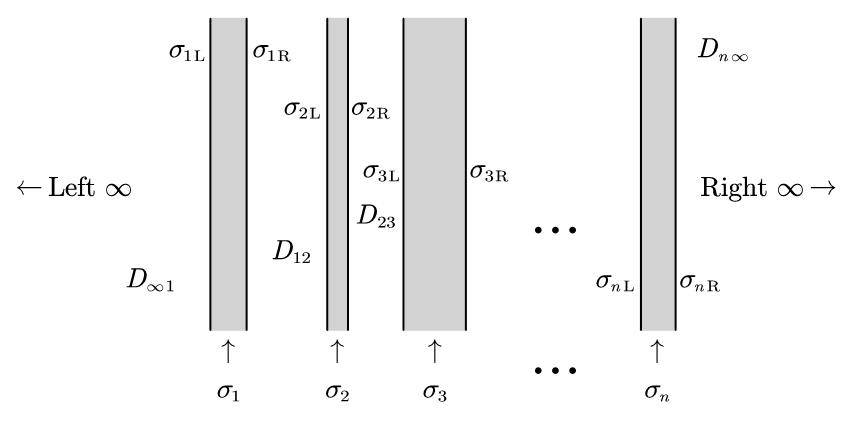
\includegraphics[width=9cm]{image/7-2-6.png}
\caption{平行板问题}\label{fig7-2-6}
\end{wrapfigure}
我们先考虑无限大的导体平面板,\,它可能具有一定的厚度.\,把这样的$n$块板子从左至右平行放置,\,如图\ref{fig7-2-6}.\,这样就把空间隔离为中间的$D_{12},\,D_{23},\,\cdots,\,D_{n-1\,n}$等区域.

我们没有必要严格写出这个问题的解.\,把这个体系的解需要满足的性质罗列出来会更实用.\,首当其冲地我们写出每一块板上的电量需要满足的关系.\,如果板非常薄,\,那么左右两侧的带电面密度$\sigma_{i{\rm L}}$和右侧$\sigma_{i{\rm R}}$就可以合成为统一的$\sigma_i$.\,那么以下两个特征是显著的:
\begin{enumerate}
\item $\sigma_{i{\rm R}}+\sigma_{i+1\,{\rm L}}=0$
\item $\sigma_{1{\rm L}}=\sigma_{n{\rm R}}=(\sigma_1+\cdots+\sigma_n)/2$
\end{enumerate}

而在第$i$与第$i+1$块板之间的区域$D_{i\,i+1}$内,\,如果研究场强,\,以向右为正.\,它应该满足两个关系:
\begin{enumerate}
\item[3.] $E_{i\,i+1}=\sigma_{i{\rm R}}/\varepsilon_0=-\sigma_{i+1\,{\rm L}}/\varepsilon_0$
\item[4.] $E_{i\,i+1}=(\sigma_1+\cdots+\sigma_i-\sigma_{i+1}-\cdots-\sigma_n)/2\varepsilon_0$
\end{enumerate}


请注意,\,在以上关系式中,\,$1,\,3$关系式仅仅依赖于上一节我们推出过的边界条件.\,是无条件成立的.\,但是$2,\,4$却无法从边界条件中推导出来.\,所以这两个式子的成立是有条件的:\,那就是整个体系``仅仅''由这些带电的板组成.\,事实上,\,如果把第$1$块板和第$n$向左向右平移到无限远,\,可以想象不改变板上的电荷分布也能保持静电平衡.\,但是这样中间就只剩下$2,\,3,\,\cdots,\,n-1$这些板,\,它们就可以造成典型的仅仅符合$1,\,3$而不符合$2,\,4$的带电体系.\,所以$2,\,4$的正确性要求``无穷远处不能有电荷分布''.\,此时我们可以通过叠加原理来解释$4$的正确性.\,又分过来通过$4$计算出来的电场强度用$3$来计算各板左右两侧的带电量.\,最后就能推导出$2$式来.

对于等式$2$,\,我们发现这实际上代表一种左右对称性:\,在这些所有板的外侧区域$D_{\infty 1},\,D_{n\infty}$观察,\,这些所有板等效于单块$\sigma_1+\cdots+\sigma_n$的板.\,从而左右的场强都是:
\[E_\infty=\frac{\sigma_1+\cdots+\sigma_n}{2\varepsilon_0}\]

\begin{wrapfigure}[10]{o}[0pt]{10cm}
\vspace{-0.2cm}
\centering
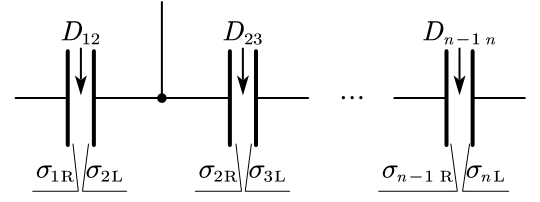
\includegraphics[width=10cm]{image/7-2-7.png}
\caption{电容器}\label{fig7-2-7}
\end{wrapfigure}
如果把上面的模型替换为电容器电路,\,各个区域$D$变成电容内部的场强区,\,而每一块导体板内部的区域被改成一根导线,\,并可以通过外界引入电量.\,那么需要注意,\,这个体系额外多了一个性质:\,\emph{一般情况下}各个电容器外侧的电量都一定是零.\,这是因为电容器初始状态必然不带电,\,而充放电过程是拟稳\footnote{即符合节点电流方程等,\,见之后章节的说明.}的,\,故两极板积累的电量必然相反.\,故按照上面的公式计算的$E_\infty$就是零.\,所以电容器极板外侧一般不允许有场强.\,除非遇到电容器中间被放置了外电荷的情况,\,比如在中间引入电压可以调控的栅极,\,对于这种``异型''电容的问题处理方法就又回到了之前我们说的四个结论上.

\vspace{0.5cm}
对于一个面积为$S$,\,极板间距为$l$的\emph{平板电容器}(parallel plate capacitor),\,正常工作的时候根据之前的结论,\,两板正对面带相反的电荷,\,电场线起始于带正电的板而终止于带负电的板.\,如果忽略其边缘效应,\,即$S\gg l$情况下,\,我们可以认为其去掉边缘以后的正对面积与$S$的相对误差非常小,\,电容就被定义为两板带正电或负电的绝对值与两板电势差的比值,\,它等于:
\[C=\frac{Q}{U}=\frac{\varepsilon_0S}{l}\]

\begin{wrapfigure}[12]{o}[0pt]{8.5cm}
\vspace{-0.5cm}
\centering
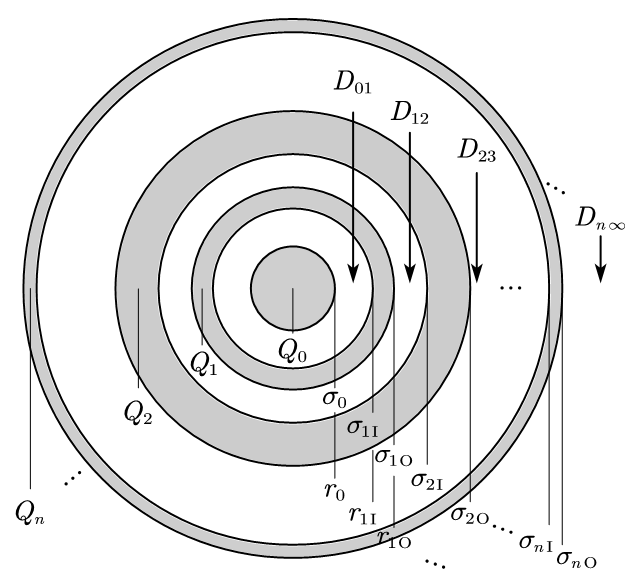
\includegraphics[width=8.5cm]{image/7-2-8.png}
\caption{球壳或柱壳}\label{fig7-2-8}
\end{wrapfigure}
当平板电容器带电时,\,其产生的能量可以通过静电能公式或计算外界做功,\,也可以用电场能量计算得到:
\[E=\frac{1}{2}CU^2=\frac{1}{2}QU=\frac{1}{2}\frac{Q^2}{C}\]

这个公式是普遍的,\,对任何符合上一个式子定义的电容都是成立的.

\vspace{1cm}
2.\,同心导体球与球壳

导体球与球壳反倒简单一些,\,它们面上的总带电量不存在发散的情况,\,而且也不需要考虑无穷远处的边界条件.\,用各内表面总带电量$Q_{\rm I}$和外表面带电量$Q_{\rm O}$描述,\,之前的四个条件现在也需要改写为:
\begin{center}\begin{minipage}{0.35\textwidth}
\begin{enumerate}
\item $Q_{i{\rm O}} +Q_{i+1\,{\rm I}}=0$
\item $Q_{n{\rm O}}=Q_1+\cdots+Q_n$
\item $E_{i\,i+1}=\dfrac{Q_{i{\rm O}}}{4\pi \varepsilon_0r^2}=-\dfrac{Q_{i+1\,{\rm I}}}{4\pi \varepsilon_0r^2}$
\item $E_{i\,i+1}=\dfrac{Q_1+\cdots+Q_i}{4\pi\varepsilon_0 r^2}$
\end{enumerate}
\end{minipage}\end{center}


两个球壳构成的电容器,\,如果内外球壳半径分别为$r_{\rm I}$和$r_{\rm O}$,\,那么电容为:
\[C=4\pi\varepsilon_0\frac{r_{\rm O}r_{\rm I}}{r_{\rm O}-r_{\rm I}}\]

\vspace{0.5cm}
3.\,共轴的导体圆柱与圆柱壳

我们先考虑无限长的圆柱.\,那么依然参考上图\ref{fig7-2-8}.\,圆柱带电应用单位长度的电量$\lambda$来描述,\,四个关系式变为:

\begin{center}\begin{minipage}{0.35\textwidth}
\begin{enumerate}
\item $\lambda_{i{\rm O}} +\lambda_{i+1\,{\rm I}}=0$
\item $\lambda_{n{\rm O}}=\lambda_1+\cdots+\lambda_n$
\item $E_{i\,i+1}=\dfrac{\lambda_{i{\rm O}}}{2\pi \varepsilon_0r}=-\dfrac{\lambda_{i+1\,{\rm I}}}{2\pi \varepsilon_0r}$
\item $E_{i\,i+1}=\dfrac{\lambda_1+\cdots+\lambda_i}{2\pi\varepsilon_0 r}$
\end{enumerate}
\end{minipage}\end{center}

两个柱壳构成的电容器,\,如果内外球壳半径分别为$r_{\rm I}$和$r_{\rm O}$,\,其长度为$l$且忽略边缘效应,\,即$l\gg r_{\rm O}>r_{\rm I}$那么电容为:
\[C=2\pi\varepsilon_0l\ln\frac{r_{\rm O}}{r_{\rm I}}\]

\section{电像法}

下面考虑两种实际的边值问题的解.\,第一种问题中区域$D$为半无限大空间,\,即,\,其边界为一个无限大导体的表面.\,第二种问题中区域$D$要么是一个球面外的延伸到无穷远的区域(外问题),\,要么是球面内的区域(内问题),\,不管哪种,\,区域边界都是导体的球面表面,\,只是前一种是外表面,\,后一种是内表面.

我们提供的方法为电像法.\,其意义是,\,先考虑一个较简单的,\,在空间中$\bs{R}$处放置一个点电荷$q$:
\[\rho(\bs{r})=q\delta(\bs{r}-\bs{R})\]

的情况下,\,边值问题的求解.\,其中$\delta(\bs{r}-\bs{R})$为\emph{狄拉克德尔塔函数}(Dirac delta function),\,读者大可以把它视作某物理量的某种极限化的密度分布的抽象\footnote{实则这样的广义函数数学上称作一种\emph{分布}(distribution),\,它是通过积分形式的运算定义的:
\[f(\bs{r}) \circ g(\bs{r}):=\int f(\bs{r})g(\bs{r})\ud V\]
\[\delta(\bs{r}-\bs{R})\circ g(\bs{r}):=g(\bs{R})\]
},\,例如物理量总值为$1$,\,分布在$\bs{R}=\bs{0}$附近的一个非常小的范围内,\,那么其密度就是:
\[\delta(\bs{r})=\begin{cases}
	+\infty &(\bs{r}=\bs{0})\\
	0	&(\bs{r}\neq \bs{0})
\end{cases} \qquad \&\quad \int\limits_{\rm Ball(\bs{0},\epsilon)} \delta(\bs{r})\ud V=1\]

那么此前的密度函数$\rho(\bs{r})=q\delta(\bs{r}-\bs{R})$就可以表示点电荷的电荷密度分布.

\subsection{半无限大空间的电像法}

下面考虑在无限大导体平板处建立坐标系,\,$z>0$就是待研究的$D$区域.\,现在在$\bs{R}$处放置一个正点电荷$q$,\,容易证明,\,由于导体板延伸到无穷远,\,所以导体板的表面自然成为第一类边界条件的表面且其电势为零$V=0$.\,表面上就会产生一个面电荷分布$\sigma(x,\,y)$.
\begin{figure}[H]
\centering
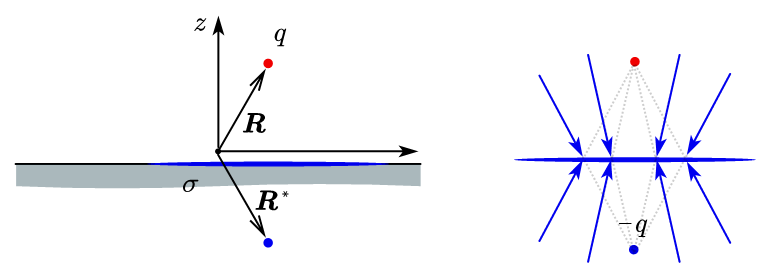
\includegraphics[width=0.7\textwidth]{image/7-2-9.png}
\caption{半无限空间的电像}
\end{figure}

见上图右,\,单独考虑这个面电荷产生的电场线,\,由于在$z<0$区域内为导体,\,合电场强度必然为零.\,故这个区域面电荷的电场线要与原来的$\bs{R}$处的$q$的电场线相抵消.\,故为指向$\bs{R}$处的汇聚的电场线.\,但是,\,由于这个面电荷产生的电场的上下的镜面对称性,\,这就导致我们可以直接证明它对$z>0$的$D$区域产生的电场线,\,实际上就相当于在$\bs{R}$的镜面对称点$\bs{R}^\ast$处放置一个\emph{像电荷}(image charge),\,值为$-q$而产生的电场.

从而$z>0$区域的电场,\,实际上就是由在$\bs{R}$的原电荷和在$\bs{R}^\ast$的像电荷共同产生的电场.\,或者说,\,满足以下方程的唯一解:
\[\nabla^2\varphi =-\frac{q\delta(\bs{r}-\bs{R})}{\varepsilon_0}\,(z>0)\quad ,\quad \varphi|_{z=0}=0\]

就是:
\[\varphi(\bs{r}) =\ke \frac{q}{|\bs{r}-\bs{R}|}-\ke \frac{q}{|\bs{r}-\bs{R}^\ast|}\]

那么我们如何求解下列更加普遍的第一类边值问题\footnote{第二类边值问题此时会有问题:\,首先导体面上的总电荷量就是上方的自由电荷量总值的相反数而不可以任意给定,\,而最终电势的结果也会产生一个未定常数的不确定性.}呢?
\[\nabla^2\varphi = -\frac{\rho(\bs{r})}{\varepsilon_0}\,(z>0)\quad ,\quad \varphi|_{z=0}=V\]

这个解答是简单的:\,就是对以上点电荷电像法的情形做叠加原理.\,我们把以上问题中,\,如果点电荷为单位电荷时,\,对应的解称作参数为$\bs{R}$处的\emph{格林函数}(Green function):
\[\delta(\bs{r}-\bs{R})\quad \longrightarrow\quad  \varphi(\bs{r})=\quad G(\bs{R},\,\bs{r})=\ke \left(\frac{1}{|\bs{r}-\bs{R}|}-\frac{1}{|\bs{r}-\bs{R}^\ast|}\right)\]

由于任意的电荷分布可以看成是点电荷的叠加,\,下式$\ud V$为$\bs{R}$改变对应的体积元:
\[\rho(\bs{r})=\int \rho(\bs{R})\delta(\bs{r}-\bs{R})\ud V\]

那么这个电荷分布产生的电势,\,就是各个点电荷的格林函数的叠加:
\[\rho(\bs{r})\quad \longrightarrow \quad \varphi(\bs{r})=\int  \rho(\bs{R})G(\bs{R},\,\bs{r})\ud V\]

这样在导体面上产生的电势依然是零,\,为了符合边界条件,\,只需要整体加上常数$V$,\,最终结果为:
\[\varphi(\bs{r})=V+\int \ke \left(\frac{1}{|\bs{r}-\bs{R}|}-\frac{1}{|\bs{r}-\bs{R}^\ast|}\right)\rho(\bs{R})\ud V\]

\subsection{球面外与球面内的电像法}

有了半无限区域的电像法求解边值问题做基础,\,我们对球面内外区域的边值问题的求解就有了线索.\,同样的,\,在球心处建立原点和坐标系,\,求解这两个问题的关键在于先求解以下两个最简单的第一类边值问题:
\[\nabla^2\varphi =-\frac{q\delta(\bs{r}-\bs{R})}{\varepsilon_0}\,(|\bs{r}|>a)\quad ,\quad \varphi|_{|\bs{r}|=a}=0\]
\[\nabla^2\varphi =-\frac{q\delta(\bs{r}-\bs{R})}{\varepsilon_0}\,(|\bs{r}|<a)\quad ,\quad \varphi|_{|\bs{r}|=a}=0\]

分别对应外问题和内问题.\,即下图左和右:
\begin{figure}[H]
\centering
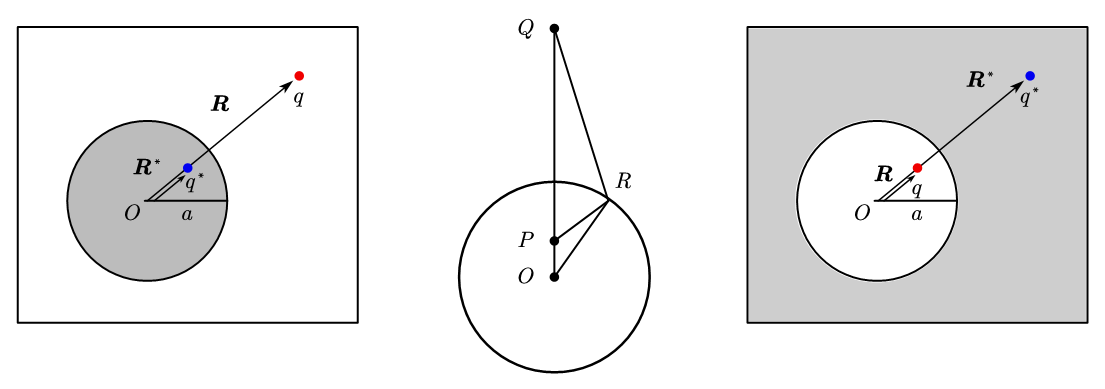
\includegraphics[width=0.8\textwidth]{image/7-2-10.png}
\caption{球面的电像}
\end{figure}

而以上两个问题的电像解,\,其实直接就都是:
\[\varphi(\bs{r}) =\ke \frac{q}{|\bs{r}-\bs{R}|}+\ke \frac{q^\ast}{|\bs{r}-\bs{R}^\ast|}\]

其中像电荷与原电荷在同一条半径上,\,且其大小$q^\ast$和到原点的距离$R^\ast$与圆的半径$a$分别满足:
\[RR^\ast=a^2\]
\[-\frac{q^\ast}{q}=\frac{a}{R}=\frac{R^\ast}{a}\]

证明这两个解的正确性的关键在于原电荷与像电荷的位置对圆是构成了一对反演点的关系.\,见上图中间的几何关系,\,不难证明:
\[\overline{OP}\cdot\overline{OQ}=a^2=\overline{OR}\quad \Rightarrow \quad \triangle OPR\sim \triangle ORQ\]

于是根据相似关系不难得到:
\[\frac{{\overline{OP}}^{1/2}}{\overline{PR}}=\frac{{\overline{OQ}}^{1/2}}{\overline{QR}}\]

所以只要让两个电荷分别位于$P,\,Q$处,\,且电荷量反号且大小之比为${\overline{OP}}^{1/2}:{\overline{OQ}}^{1/2}$,\,那么它们在$R$处的电势和就是零.\,实际上上面的电势解就是取了这样的两个电荷的电势的和,\,故就能满足原来的方程的边界条件,\,而这样的电势恰好在给定区域$D$内也能满足对应的微分方程:\,即$\nabla^2\varphi$只得到$\bs{R}$处电荷$q$.

这就证明了以上写出来的解是正确的.\,根据唯一性定理,\,它也是唯一的.

\vspace{0.5cm}
下面考虑在普遍的第一类和第二类边值问题下外问题的解.\,先考虑第一类边值问题,\,即:
\[\nabla^2\varphi = -\frac{\rho(\bs{r})}{\varepsilon_0}\,(|\bs{r}|>a)\quad ,\quad \varphi|_{|\bs{r}|=a}=V\]

同样的是利用以上解写出格林函数:
\[\quad G(\bs{R},\,\bs{r})=\ke \left(\frac{1}{|\bs{r}-\bs{R}|}-\frac{a/|\bs{R}|}{|\bs{r}-\bs{R}^\ast|}\right)\]

于是只需要写出下列积分,\,就可以满足问题前一半的拉普拉斯方程:
\[\int \rho(\bs{R})G(\bs{R},\,\bs{r})\ud V \]

这样一个势在边界上必然取零的值.\,为了使得最后的解满足边界条件,\,自然去思考叠加原理:\,让外界$\rho=0$且边界上具有电势$V$的电势显然为:
\[\varphi=\frac{VR}{r}\]

故,\,最后的解就是:
\[\varphi=\frac{VR}{r}+\int \ke \left(\frac{1}{|\bs{r}-\bs{R}|}-\frac{a/|\bs{R}|}{|\bs{r}-\bs{R}^\ast|}\right)\rho(\bs{R})\ud V\]

但是如果换为第二类边值问题:
\[\nabla^2\varphi = -\frac{\rho(\bs{r})}{\varepsilon_0}\,(|\bs{r}|>a)\quad ,\quad \int\limits_{|\bs{r}|=a}\nabla\varphi\cdot \ud \bs{S}=Q\;,\;\varphi|_{|\bs{r}|=a}=C\]

这就需要先考虑格林函数对应的势在边界上产生的总面电荷量,\,他其实就是像电荷的值:
\[\delta(\bs{r}-\bs{R})\quad \longrightarrow\quad  \int\limits_{|\bs{r}|=a}\nabla\varphi\cdot \ud \bs{S}=-\frac{a}{|\bs{R}|}\]

于是单独对格林函数进行积分得到的电势就使得面上带上电荷:
\[\rho(\bs{r})\quad \longrightarrow\quad \int\limits_{|\bs{r}|=a}\nabla\varphi\cdot \ud \bs{S}=-\int \frac{a}{|\bs{R}|}\rho(\bs{R})\ud V\]

那么通过叠加原理,\,为了使得面上电荷量变为$Q$,\,就需要引入一个电势:
\[\varphi=\ke \frac{Q+\displaystyle\int \frac{a}{|\bs{R}|}\rho(\bs{R})\ud V}{r}\]

综上,\,最后的解为:
\[\varphi =\ke \frac{Q+\displaystyle\int \frac{a}{|\bs{R}|}\rho(\bs{R})\ud V}{r}+\int \ke \left(\frac{1}{|\bs{r}-\bs{R}|}-\frac{a/|\bs{R}|}{|\bs{r}-\bs{R}^\ast|}\right)\rho(\bs{R})\ud V \]

球面外问题中,\,所有电势的结果都是$\rho(\bs{r})$和球面上的面电荷分布通过叠加原理产生的电势.

最后考虑内问题.\,我们介绍过,\,此时只有唯一的一种情况:\,即内表面取为电势为零的第一类边界条件.\,其问题表述和解必然为:
\[\nabla^2\varphi = -\frac{\rho(\bs{r})}{\varepsilon_0}\,(|\bs{r}|<a)\quad ,\quad \varphi|_{|\bs{r}|=a}=0\]
\[\varphi=\int \ke \left(\frac{1}{|\bs{r}-\bs{R}|}-\frac{a/|\bs{R}|}{|\bs{r}-\bs{R}^\ast|}\right)\rho(\bs{R})\ud V\]

这个电势就是内部的电荷$\rho(\bs{r})$和面上的感应面电荷共同对球内叠加产生的电势的和.\,对于球外的电势的叠加必然为零.

\subsection{几种其他情况*}

\vspace{0.2cm}
1. 球谐函数
\vspace{0.2cm}

将一个中心在原点$\bs{r}=\bs{0}$,\,半径为$a$的球置于外场中讨论静电平衡为上一节中外问题的设置.\,但是上一节选择了在距离球心$R$处放置了一个点电荷.\,从而得到了球面在点电荷产生的外场下形成的格林函数$G(\bs{R},\,\bs{r})$.\,实用问题中通常把外场按照\emph{立体谐函数}(solid harmonics)在原点进行分解,\,类似于泰勒展开.\,只不过立体谐函数更适合于球坐标:
\[R_{lm}(\bs{r})=\sqrt{\frac{(l-m)!}{(l+m)!}}r^lP_{lm}(\cos\theta)e^{\ui m\varphi}\]
\[P_{lm}(x)=(-)^m(1-x^2)^{m/2}\frac{\ud^mP_l(x)}{\ud x^m}\]
\[P_l(x)=\frac{(-)^l}{2^ll!}\frac{\ud^l}{\ud x^l}(1-x^2)^l\]

这样的复杂定义其实非常自然地缘起于球坐标下拉普拉斯方程的解.\,除了以上\emph{正规}(regular)部分,\,还有一组对应的在原点发散的\emph{非正规}(irregular)解:
\[I_{lm}(\bs{r})=\sqrt{\frac{(l-m)!}{(l+m)!}}r^{-(l+1)}P_{lm}(\cos\theta)e^{\ui m\varphi}\]

非正规解作为电势代表的场由放在原点的电荷,\,电偶极子乃至更高阶的对象产生.\,因为我们在原点放置了一个导体球, 所以它受到的外场不可能含有非正规成分.

以上完备谐函数组非常复杂,\,实际我们考虑的问题通常对球坐标$\varphi$的改变是对称的,\,例如球外点电荷对原点附近的外场,\,若以原点和点电荷的连线方向为极轴定义$\theta,\,\varphi$,\,那么这个外场就不含任何立体谐函数中$m\neq 0$的成分.\,此时仅考虑$m=0$的那些函数是完备的:
\[R_l(\bs{r})=\frac{1}{2^ll!}\cdot{r^l}\cdot\left(\frac{\ud}{\sin\theta\ud \theta}\right)^l\sin^{2l}\theta\]
\[I_l(\bs{r})=\frac{1}{2^ll!}\cdot\frac{1}{r^{l+1}}\cdot\left(\frac{\ud}{\sin\theta\ud \theta}\right)^l\sin^{2l}\theta\]

对于较小的$l$我们罗列若干对称立体谐函数:
\begin{table}[H]
\centering
\def\arraystretch{2}
\begin{tabular}{c|c|c}
\hline
l	&正规	&非正规 \\
\hline\hline
0	&$1$	&$\dfrac{1}{r}$\\\hline
1	&$r\cos\theta$	&$\dfrac{\cos\theta}{r^2}$\\\hline
2	&$\dfrac{r^2}{2}(3\cos^2\theta-1)$	&$\dfrac{1}{2r^3}(3\cos^2\theta-1)$\\\hline
3	&$\dfrac{r^3}{2}(5\cos^3\theta-3\cos\theta)$	&$\dfrac{1}{2r^4}(5\cos^3\theta-3\cos\theta)$\\\hline
4	&$\dfrac{r^4}{8}(35\cos^4\theta-30\cos^2\theta+3)$	&$\dfrac{1}{8r^5}(35\cos^4\theta-30\cos^2\theta+3)$\\\hline
$\vdots$&$\vdots$&$\vdots$\\\hline
\end{tabular}
\caption{对称立体谐函数表}
\end{table}

值得注意的是,\,正规的立体谐函数总是可以写成多项式的形式.\,如果以$\theta=0$的方向为$z$轴,\,那么$r\cos\theta=z,\,r^2=x^2+y^2+z^2$.\,这样就得到了对称情况下的\emph{谐和多项式}(harmonic polynomials),\,例如:
\begin{align}
R_0(\bs{r})=\mathcal{P}_0(x,\,y,\,z)	&=1\\
R_1(\bs{r})=\mathcal{P}_1(x,\,y,\,z)	&=z\\
R_2(\bs{r})=\mathcal{P}_2(x,\,y,\,z)	&=\frac{2z^2-(x^2+y^2)}{2}\\
R_3(\bs{r})=\mathcal{P}_3(x,\,y,\,z)	&=\frac{2z^3-3z(x^2+y^2)}{2}\\
R_4(\bs{r})=\mathcal{P}_4(x,\,y,\,z)	&=\frac{35z^4-30z^2(x^2+y^2)-3(x^2+y^2)^2}{8}\\
&\vdots
\end{align}

不难验证它们都会符合拉普拉斯方程:
\[\left(\frac{\partial^2}{\partial x^2}+\frac{\partial^2}{\partial y^2}+\frac{\partial^2}{\partial z^2}\right)\mathcal{P}_l(x,\,y,\,z)=0\]

就是这样一些正规立体谐函数代表的电势,\,如果作为外场施加在置于原点的接地导体球上,\,应该得到怎样的静电平衡结果呢?\,首先我们明确这种场合下第一类边值问题表述为:
\[\nabla^2\varphi=0(|\bs{r}|>a)\quad ,\quad \varphi|_{|\bs{r}|=a}=0 \quad ,\quad \varphi|_{|\bs{r}|\to+ \infty}=\lambda R_l(\bs{r})\]

由于正规立体谐函数电荷摆放于无穷远处,\,而球面上感应电荷产生的电势在无穷远处影响一次反比于半径,\,故此时边界条件变成了一个\emph{渐进边值条件}(asymptotic boundary condition),\,它规定了半径趋近于无穷远时电势函数的变化趋势.

这个方程的解非常平庸地等于同阶的非正规立体谐函数与原来的正规谐函数的叠加:
\[\varphi(\bs{r})=\lambda R_l(\bs{r})+\mu I_l(\bs{r})\]

这是非常显然的.\,同阶的正规与非正规谐函数关于角度的部分变化趋势是一致的,\,为了满足在球面上电势为零的边值条件,\,我们只需要把半径取$a$并视作系数,\,再要求两个系数抵消,\,这只需要要求:
\[a^l\lambda+\frac{\mu}{a^{l+1}}=0\]

从而马上得到$\mu=-a^{2l+1}\lambda$.\,或者更简单地,\,我们把以下电势作为这一类问题的基础解:
\[\varphi=\frac{Q}{2^ll!\cdot 4\pi\varepsilon_0 a}\cdot\left[\left(\frac{a}{r}\right)^{l+1}-\left(\frac{r}{a}\right)^l\right]\cdot\left(\frac{\ud}{\sin\theta\ud \theta}\right)^l\sin^{2l}\theta\]



\section{电介质}

之前介绍过,\,绝缘体只有考虑漏电或是大电场下击穿时,\,导电才得以发生.\,但这绝对不意味着忽略导电现象以后绝缘体对于静电场没有任何响应.\,这时发生的一个重要的现象为\emph{极化}(polarization).\,它会造成很多独特现象:\,从在头发上摩擦过的塑料笔杆对小纸屑的吸引\footnote{用金属屑的静电平衡也可以实现,\,不过金属屑密度大现象更不明显.},\,到电气工业大电容器的制作,\,更广义地说,\,在交变电场中介质的极化最终还能决定电磁波或光在介质中的传播,\,下一章我们将首次小小讨论以下这个问题.\,我们把明显能产生极化的介质称作\emph{电介质}(dielectrics).\,极化的含义可以从微观和宏观两个角度来考虑,\,背后涉及物理学的多个方面.\,我们分别进行讨论.\,最后揭示微观角度与宏观角度极化规律的联系.\,

\subsection{微观角度理解极化}

固体或晶体,\,尤其是离子晶体或部分共价晶体,\,每一个原子实际上本身就带电,\,其极化机理非常复杂,\,需要用到爱因斯坦,\,玻恩,\,黄坤等人的陆续完善的理论.\,或是放弃研究微观机理,\,通过宏观的方式引入唯象的描述方法.\,我们下面研究的主要是由原子,\,分子构成的气体或者液体的极化.

在这样的场合下,\,每一个单元被单独研究,\,原子或分子整体是没有电性的,\,但是正如之前所说的,\,下式决定的原子或分子的电偶极矩不必为零:
\[\bs{p}=\int \rho \bs{r} \ud V\]

如果从非量子的经典物理观点(包括半经典的玻尔模型)来看,\,即使简单如氢原子,\,看作轻的电子绕近似不动的质子做匀速圆周运动,\,每一个瞬时也会形成一个电偶极矩.\,但是它随时间快速转动而导致在静电场意义下其平均值为零.\,事实上,\,量子力学认为无论哪一个时刻,\,氢原子都处于电偶极矩沿任何方向概率都相等的\emph{定态}(stationary state),\,并没有在随时间演变.\.所以无论是从理论上来看还是从实际上来看,\,孤立氢原子基态下总是不体现电偶极矩的:
\[\overline{\bs{p}}=\bs{0}\]

具有这样性质的分子就称作\emph{无极分子}或\emph{非极性分子}(nonpolar molecule),\,反之则称作\emph{有极分子}或\emph{极性分子}(polar molecule)一般可以通过化学原理给出分子的成键和立体构型加以判断.\,例如${\rm CO}$分子和${\rm H_2 O}$具有极性而${\rm CO_2}$分子和${\rm CH_4}$则是无极的.

现在把无极分子放在外电场中,\,情况就会发生戏剧性的转变:\,把无极分子感受到的局部的电场视作匀强场,\,这个外场记做$\bs{E}'$.\,即使是简单如氢原子,\,其平均电偶极矩也不应当再视作零.\,这一个现象有若干解释方法:

\begin{enumerate}
\item 最唯象的解释方法把氢原子视作一个由劲度系数$k$的弹簧连接的作为正电负电中心的质点构成的体系,\,带电量为$\pm e$.\,但是忽略正负电荷之间的电相互作用力,\,只用去考虑受到的外力与等效电相互作用出来的线性弹性力的平衡,\,那么自然平衡时从负电荷到正电荷具有位移:
\[\bs{r}=\frac{e\bs{E}'}{k}\]

从而得到分子平均电偶极矩:
\[\overline{\bs{p}}=e\bs{r}=\frac{e^2}{k}\bs{E}'\]

\item 一个具有可证伪性的结果由以下考虑描述.\,通过量子理论的计算,\,把原子外的电子看作电子云,\,它是一个总电量为$-e$的连续电荷密度分布:
$$
\rho =\frac{-e}{\pi a_{0}^{3}}\ue^{-\frac{2r}{a_0}}
$$

其中$a_0=5.3\times 10^{-11}{\rm m}$为玻尔半径.\,进一步假设这个电荷分布为彻底刚性的.\,在外电场作用下,\,仅仅是原来在原点的质子现在位移到了$\bs{r}$处.\,质子对电子云的力就是电子云对质子的力,\,它与外电场力平衡.\,这样计算可以得到:
\[\bs{r}=\frac{3\pi\varepsilon_0 a_0^3}{e}\bs{E}\quad ,\quad \overline{\bs{p}}=3\pi\varepsilon_0 a_0^3\bs{E}'\]

\item 以上结果仅仅是与实验测量结果数量级一致,\,但是差了$6$倍,\,即实验结果表明:
\[\overline{\bs{p}}=18\pi\varepsilon_0 a_0^3\bs{E}'\]

这是因为上一个做法中认为电子云不会发生任何改变,\,反倒是质子位移了的做法不符合事实.\,正确的做法反而需要依然以质子为原点去解库仑场与弱匀强电场下电子的薛定谔方程的微扰解.\,这样才可以给出电子云的新分布.\,同样的计算也会带来著名的\emph{斯塔克效应}(Stark effect).\,即玻尔模型对应的第$n$能级(第$n-1$激发态)现在将分裂为$2n-1$个能级.\,进而影响谱线.

\end{enumerate}

不管用何种方式解释,\,以上现象就是第一种极化机理,\,称作\emph{位移极化}(distorsion polarization).\,它的结果为每一个分子产生了一个量子平均的电偶极矩,\,在弱场下这个电偶极矩应当正比于电场强度:
\[\overline{\bs{p}}=\alpha \bs{E}'\]

其中$\alpha$称作\emph{分子极化率}(molecular polarizability).\,它是表征微观极化难易程度的重要参数.\,对于位移极化,\,分子极化率是一个量子行为的结果,\,从氢原子的极化率就可以看出,\,因为玻尔半径$a_0$的计算依赖于普朗克常数的取值:
\[\alpha =18\pi\varepsilon_0 a_0^3=\frac{9(4\pi\varepsilon_0)^4\hbar^6}{2m_e^3e^6}=7.42\times 10^{-41} {\rm F\cdot m^2}\]
\vspace{1cm}

而对于有极分子,\,分子即使在没有外场作用时,\,由于其电荷分布本身就会造成一个电偶极矩,\,称作\emph{固有电偶极矩}(permanent dipole moment),\,我们记做$p_0$,\,但是由于无规则的热运动,\,其方向$\bs{e}$是随机的,\,所以作为每个分子的电偶极矩矢量$\bs{p}=p_0\bs{e}$的统计平均,\,其结果依然应当为$\bs{0}$:
\[\overline{\bs{p}}=\bs{0}\]

\begin{wrapfigure}[11]{o}[0pt]{6cm}
\vspace{-0.2cm}
\centering
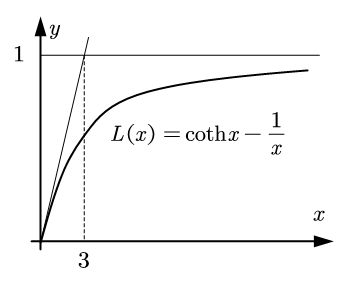
\includegraphics[width=6cm]{image/7-2-11.png}
\caption{郎之万函数}\label{fig7-2-11}
\end{wrapfigure}
现在施加外电场$\bs{E}'$以后,\,如果认为分子依然保持刚性,\,即$p_0$不变,\,但方向可以自由转动,\,则与电场保持同向的电偶极子的势能得到降低,\,电偶极子在动力学上倾向于与外电场同向排列.\,但是其热运动越剧烈,\,转动动能就越大,\,不同电偶极子相互影响就会使得其排列趋于杂乱无章.\,忽略可能的量子效应,\,由玻尔兹曼分布可以得到在温度为$T$时分子沿电场方向的平均电偶极矩:
\[\overline{p}=p_0\left({\rm coth}\,\frac{pE'}{kT}-1\middle/\frac{pE'}{kT}\right)\]

一般把上面这个函数称作\emph{郎之万函数}Langevin function),\,即:
\[\overline{p}=p_0 L\left(\frac{pE'}{kT}\right)\quad,\quad L(x)={\rm coth}\,x-\frac{1}{x}\]

这个函数的图像如\ref{fig7-2-11}所示.\,它有两条渐近线,\,分别对应两种具体的物理情形:

如果低温($T$很小)或者强场($E'$很大)但不至于漏电或击穿.\,使得宗量$x=pE'/kT\gg 1$,\,那么就使用水平$y=1$渐近线,\,即:
\[\overline{p}\approx p_0\]

对应几乎所有电偶极子都沿电场方向排列的\emph{饱和极化}(saturated polarization)情况.

如果高温($T$很大)或者弱场($E'$很小).\,使得宗量$x=pE'/kT\ll 1$,\,那么就使用原点切线$y=x/3$的渐近线,\,即:
\[\overline{p}\approx \frac{p_0^2}{3kT}E'\]

写成矢量式,\,我们发现与位移极化得到了相似的结果:
\[\overline{\bs{p}}=\alpha \bs{E}'\quad,\quad \alpha =\frac{p_0^2}{3kT}\]

这被称作\emph{郎之万-德拜定律}(Langevin-Debye law).\,同样地把$\alpha$称作分子极化率.\,而这种极化机理称作\emph{取向极化}(orientation polarization).\,取向极化的极化率是一个热学行为的结果,\,从极化率反比于温度这一点就可以看出来.

\vspace{1.5cm}

关于取向极化和位移极化我们总结以下几点:

一是要注意两者的不同:\,前者是外电场诱导产生或改变固有电偶极矩,\,是一个量子行为,\,几乎不依赖于温度.\,后者是外电场诱导固有电偶极矩选取优势方向,\,是一个热学现象,\,定性解释不依赖于量子特性.\,但是严格说来温度对前者也会有非常微小的影响,\,低温下量子特性对后者也会有不小的改变.

二是要注意两者可以同时出现:\,无极分子当然只能采取位移极化.\,但有极分子的取向极化和位移极化是并存的.\,所以分子极化率的完整计算方法为分别考虑两种极化方式带来的系数的和:
\[\alpha=\alpha_{\rm dis}+\alpha_{\rm ort}\]

三是要注意具体情况主要考虑哪一种极化方式:\,一般说来,\,有极分子的极化率中取向极化远大于位移极化的贡献\footnote{使分子转向导致的能量差小,\,使电子在不同能级间跃迁需要的能量差大,\,前者易后者难.},\,故有极分子的极化主要是取向极化.\,但是无极分子,\,位移极化就取代取向极化称为唯一需要考虑的极化因素了,\,故静电场下其分子极化率一般比有极分子要小一个量级.\,但是对于高频电场,\,\emph{弛豫时间}(relaxation time)成为了另一个需要考虑的重要因素.\,大约对于超过红外线频率的电场下,\,取向的改变就难以跟上电场的变化频率了,\,这导致介质的极化转而成为了电子的位移极化,\,考虑介质对光的色散和吸收都是基于这一点的.

\subsection{宏观角度理解极化}

之前章节已经介绍过极化强度$\bs{P}$的定义与相关的性质.\,宏观上的极化规律指的是,\,如果介质内部某点处局域地存在(平均意义下的)场强$\bs{E}$,\,那么该点就局域地产生一个极化强度$\bs{P}$,\,做为$\bs{E}$的响应函数:
\[\bs{P}=f(\bs{E})\]

这样的函数实际上或是应用上都不一定是线性的,\,但是在各向同性介质,\,弱场,\,低频的三个条件下,\,理论或实验都能给出线性的结果,\,一般写为:
\[\bs{P}=\chi_e \varepsilon_0 \bs{E}\]

这样$\chi_e$就是只与材料和环境(温度,\,压强)有关的,\,而与外加电场大小与方向无关的无量纲标量常数.\,称作\emph{极化率}(susceptibility).

类似于导体的静电平衡问题,\,介质的极化是如何达到平衡的?,\,这一个问题也应当动态地去思考:\,对比导体中的平衡条件$\bs{E}=\bs{0}$,\,介质中的上平衡条件也不过是一个最终才能达到的结果,\,达到平衡前的弛豫过程,\,等号不一定要成立.\,导体未平衡时,\,内部正是因为有电场才驱使电荷定向运动从而转移,\,从而电场才被改变,\,在改变中逐渐趋于零.\,那么介质也是类似:\,如果把一块未被极化的介质置于外电场$\bs{E}_0$中,\,一开始$\bs{P}=\bs{0}$将小于预期的$\chi_e \varepsilon_0 \bs{E}_0$值,\,那么极化就会慢慢发生,\,$\bs{P}$开始增大,\,位移极化和取向极化在逐渐发生,\,宏观看会产生\emph{极化电流}(polarization current),\,不难验证其电流密度为$\bs{J}_P=\partial \bs{P}/\partial t$.\,但是由于$\bs{P}$的变化,\,势必会在介质表面甚至内部产生极化电荷分布$\sigma_P,\,\rho_P$.\,这些电荷产生的场将部分抵消原来的外电场,\,称作\emph{退极化场}(depolarization field).\,于是$\bs{E}_0$也将动态的变化到最终的$\bs{E}$,\,使得以上平衡方程成立.\,这样极化强度就不再增加.

所以同样的以极化平衡条件$\bs{P}=\chi_e \varepsilon_0 \bs{E}$为出发点,\,应当期望可以类似于导体静电平衡那样得到有效的求解带电介质的静电平衡问题.\,但是由于平衡条件更复杂,\,我们的方法也需要进行改进.\,事实上不难验证改进的方法取$\chi_e\to+ \infty$就会退化为导体的情况.\,所以改进的方法反而更具有普遍性.

最核心的一点是引入辅助的\emph{电位移}(electric displacement)矢量来简化问题.\,这个矢量被定义为:
\[\bs{D}=\varepsilon_0 \bs{E}+\bs{P}\]

用$\bs{D}$的值反过来计算反映极化的$\bs{P}$,\,这会带来两个好处,\,第一是,\,极化规律的平衡条件被等价地写作:
\[\bs{D}=\varepsilon_0 \bs{E}+\chi_e \varepsilon_0 \bs{E}=\varepsilon_r \varepsilon_0 \bs{E}=\varepsilon \bs{E}\]

同样的$\varepsilon_r=1+\chi_e$也会作为一个基本常数,\,与原来的极化规律的结构复杂度一致.\,这个常数称作\emph{相对介电常数}(relative permittivity),\,其与真空介电常数$\varepsilon_0$的乘积$\varepsilon=\varepsilon_r \varepsilon_0$则称作\emph{绝对介电常数}(absolute permittivity)或简单称作\emph{介电常数}(permittivity).\,合理的极化率应当为正数,\,而根据相对介电常数的定义,\,它则要是大于$1$的正数.\,而介电常数的实用程度大于极化率的实用程度.

第二个关键的好处是,\,我们已经知道,\,$\bs{E}$与电荷通过高斯定理联系,\,而$\bs{P}$与极化电荷也可以通过高斯定理联系:
\[\nabla\cdot \bs{E}=\frac{\rho}{\varepsilon_0}\quad ,\quad \nabla\cdot \bs{P}=-\rho_P\]

代入刚才的电位移的定义马上就可以发现:
\[\nabla \cdot \bs{D}=\rho_f\]

即,\,电位移通过高斯定理联系的电荷就是``自由''电荷.\,这里的``自由''不是指导体中或导体表面的电荷,\,恰恰相反,\,如果把导体静电平衡问题中的导体也视作$\varepsilon_r\to+ \infty$的特殊电介质,\,这些电荷反倒要被排除.\,$\rho_f$的含义通过推导上式使用的关系式$\rho_f=\rho-\rho_P$就很容易看出来了,\,表示除去介质极化产生的面电荷或体电荷以外的一切电荷,\,一般都是置于介质外部区域的给定电荷,\,但对于介质情况它也可以分布在介质内.

对于带介质的静电平衡问题的求解就有了两种思路,\,第一种思路仅仅适用于比较简单的情况,\,这种情况不需要借助我们引入的电位移矢量$\bs{D}$就能得到结果.\,分别是把无限大块状介质和介质球放在匀强电场$\bs{E}_0$中的求解:

\begin{figure}[H]
\centering
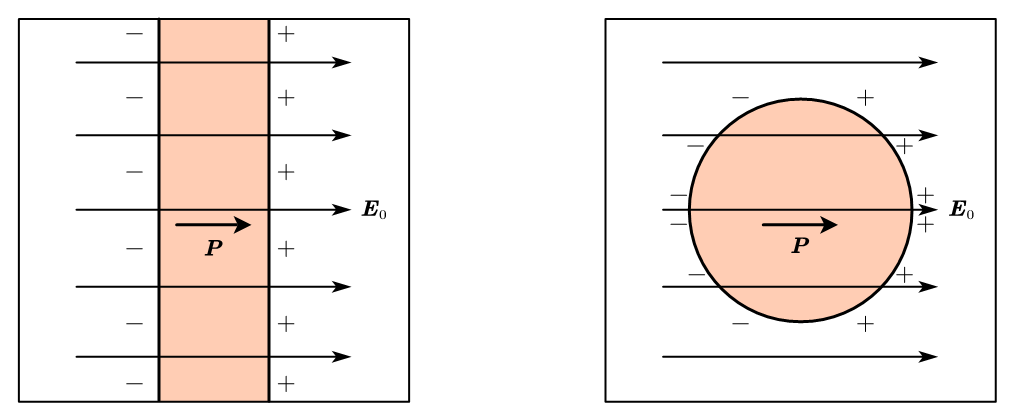
\includegraphics[width=0.6\textwidth]{image/7-2-12.png}
\caption{两种简单情况}
\end{figure}

这两个问题的核心在于大胆猜测介质内部是均匀极化的.\,设极化强度为$\bs{P}$.\,对于平板介质块,\,极化电荷在两侧产生的电荷面密度$\pm \sigma_P$就是:
\[\sigma_P=P\]

从而在介质内部形成的退极化场就是:
\[\bs{E}_P=-\frac{\bs{P}}{\varepsilon_0}\]

从而极化规律导致:
\[\bs{P}=\chi_e \varepsilon_0 \bs{E}=(\varepsilon_r-1)\varepsilon_0\left( \bs{E}_0 -\frac{\bs{P}}{\varepsilon_0}\right)\]

这就解出了平衡时的极化强度:
\[\bs{P}=\frac{\varepsilon_r-1}{\varepsilon_r}\varepsilon_0 \bs{E}_0\]

我们关心的是介质内部的电场强度:
\[\bs{E}=\bs{E}_0 -\frac{\bs{P}}{\varepsilon_0}=\frac{ \bs{E}_0}{\varepsilon_r}\]

这个结论很贴切地反应了$\varepsilon_r$的物理意义:\,它是简单的平板情况下介质对电场的削弱.\,故对于导体情况,\,内部电场强度在静电平衡时被削弱为零,\,故可以视作$\varepsilon_r\to +\infty$.

\begin{wrapfigure}[10]{o}[0pt]{7cm}
\vspace{-0.2cm}
\centering
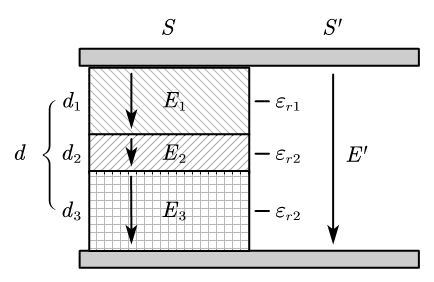
\includegraphics[width=7cm]{image/7-2-13.png}
\caption{电容器}\label{fig7-2-13}
\end{wrapfigure}
注意到这样的$\pm\sigma_P$在介质块外场强为零,\,故不影响外界.\,从而如果把多块介质块叠放,\,不同介质块就相当于按照不同的相对介电常数去削弱同一个电场.\,也就是说如图\ref{fig7-2-13}的三个介质块上方下方的导体板上的电荷面密度如果为$\sigma$,\,就会有:
\[E_0=\frac{\sigma}{\varepsilon_0}\quad ,\quad \varepsilon_{r1}E_1=\varepsilon_{r2}E_2=\varepsilon_{r3}E_3=E_0\]

但是要注意,\,这个$E_0$不一定要与旁边的空间中的$E'$相等,\,即在$S$和$S'$面上的电荷面密度没有必要是相等的,\,同一个表面的带电可以不均匀.\,而$E_i,\,i=1,\,2,\,3$也没有必要等于$E_0$,\,这不会与电场的环路定理矛盾,\,因为在介质块的边缘电场实际上已经不能视作匀强电场,\,而这一点作为边缘效应被我们忽略了.\,只有以下等势条件式是必须成立的:
\[E_1d_1+E_2d_2+E_3d_3=E'd=U\]

除了严格把以上量都解出来,\,我们讨论这个体系的静电平衡时经常会把它看做电容,\,每一个电容的性质和值由以下关系描述:
\[Q=CU\quad ,\quad C=\frac{\varepsilon S}{d}\]

注意电容器的并联等效电容应当满足直接求和的关系,\,串联反倒需要用电阻并联的方式来计算:
\[C_{\rm series}=C_1+C_2\quad ,\quad C_{\rm parallel}=C_1\parallel C_2=\frac{C_1C_2}{C_1+C_2}\]

于是上一个问题的总电容就是:
\[C=(C_1\parallel C_2\parallel C_3)+C'\]

现在让我们关心一下在三个介质中的电位移矢量,\,就会发现:
\[D_1=D_2=D_3=\varepsilon_0 E_0=\sigma\]

可以发现电位移与忽略电介质时的电场其实就差一个物理常数$\varepsilon_0$.\,它的存在可以理解为仅仅为了统一量纲.

\vspace{0.8cm}

现在让我们看介质球的极化问题.\,此时均匀的极化为球的表面带来的电荷面密度就变成了$\sigma_P=P\cos\theta$,\,而如上一章所述,\,这样的电荷分布带来的退极化场为:
\[\bs{E}_P=-\frac{\bs{P}}{3\varepsilon_0}\]

仅为块状情况的三分之一.\,可以想见,\,其极化会更加的强.\,事实上平衡方程与解变为:
\[\bs{P}=(\varepsilon_r-1)\varepsilon_0\left( \bs{E}_0 -\frac{\bs{P}}{3\varepsilon_0}\right)\quad \Rightarrow \quad \bs{P}=\frac{3(\varepsilon_r-1)}{\varepsilon_r+2}\varepsilon_0\bs{E}_0\]

那么球内的电场就被削弱到了:
\[\bs{E}= \bs{E}_0 -\frac{\bs{P}}{3\varepsilon_0}=\frac{3}{\varepsilon_r+2}\bs{E}_0\]

可见此时$\varepsilon_r$就没有体现出它的物理意义来:\,它并不能代表任意情况下介质对外加电场的削弱的比例,\,这里被削弱的比例变成了:
\[\epsilon=\frac{\varepsilon_r+2}{3}\]

从而这种情况下研究电位移表面上看上去没有意义:
\[\bs{D}=\varepsilon_0 \bs{E}+\bs{P}=\frac{3\varepsilon_r}{\varepsilon_r+2}\varepsilon_0\bs{E}_0\]

其实不然,\,下面我们来看带电介质的静电平衡问题的第二种思路,\,它也是普遍问题的处理思路,\,主要就是需要借助电位移矢量来考虑问题的.

\vspace{1cm}

首先,\,在同一种介电常数为$\varepsilon$的介质中,\,我们抛弃极化矢量$\bs{P}$,\,用电场强度$\bs{E}$和电位移$\bs{D}$可以完备地表达出极化平衡以后的场与荷(下面默认去除极化电荷,\,平衡的时候极化电荷的值是有唯一解的未知量)关系,\,它由三个关系构成:
\[\bs{D}=\varepsilon\bs{E}\]
\[\begin{cases}\;\nabla \cdot\bs{D}=\rho\\ \; \nabla \times\bs{E}=0\end{cases}\quad \text{或}\quad \begin{cases}\displaystyle\;\;\oint\limits_{\partial V} \bs{D}\cdot \ud \bs{A}=\int\limits_V\rho\ud V\\  \displaystyle\;\;\oint\limits_{\partial A} \bs{E}\cdot \ud \bs{l}=0\end{cases}\]

第一个式子称作电介质的\emph{本构方程}(constitutive equation).\,后两个式子就是介质中的高斯定律和环路定律.\,实际上还缺少一个势与它们的关系,\,势与场之间的关系不需要做任何改变:
\[\bs{E}=-\nabla \varphi\]

从而很容易得到势与荷之间的关系,\,现在变为:
\[\nabla^2\varphi=-\frac{\rho}{\varepsilon}\]

那么现在我们考虑电介质的静电平衡问题的表述方法.\,与导体静电平衡的区别在于,\,除了各真空区域$\varepsilon=\varepsilon_0$的电势分布待解以外,\,各个介质内部的电势分布也是待解的,\,我们甚至可以把外电荷引入介质的内部.\,这样我们索性就把空间按大块介质分成不同不相交的区域$D_i$的并:
\[\mathbb{R}^3=\bigcup_i D_i\]

每一个区域内部的介电常数为$\varepsilon_i$.\,而待解的电势为$\varphi_i$,\,如果该区域内有外电荷分布$\rho(\bs{r})$,\,则在介质内部需要满足:
\[\nabla^2\varphi(\bs{r})|_{\bs{r}\in D_i}=-\frac{\rho(\bs{r})}{\varepsilon_i}\]

但是凭以上方程不足以确定整个问题,\,一般还需要配合\emph{边界条件}(boundary relation).\,介质静电平衡问题的边界条件有它独特的重要性,\,一般会做如下表述:

\begin{wrapfigure}[8]{o}[0pt]{6cm}
\vspace{-0.9cm}
\centering
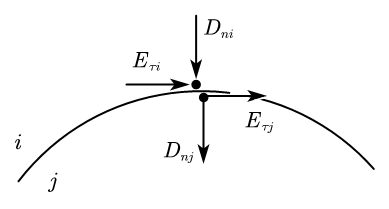
\includegraphics[width=6cm]{image/7-2-14.png}
\caption{边界条件}\label{fig7-2-14}
\end{wrapfigure}
如图\ref{fig7-2-14},\,在介质$i,\,j$的分界面上,\,把$i$指向$j$为正方向的场的法向分量的电位移记为$D_{ni},\,D_{nj}$.\,而切向分量以其自然方向为正方向的电场强度记做$E_{\tau i},\,E_{\tau j}$.\,如果面上没有外电荷,\,只有极化电荷,\,那么根据高斯定律和环路定律,\,容易得到:
\[D_{ni}=D_{nj}\quad ,\quad E_{\tau i}=E_{\tau j}\]

通常称作:\,\emph{法向电位移连续,\,切向电场强度连续.}

但是面上如果有$\sigma_{ij}$的外电荷,\,第一个式子就必须改为:
\[D_{nj}-D_{ni}=\sigma_{ij}\]

用这样的方程来确定平板电容器或其他具有高对称性电容器中的场分布非常方便.\,即使是之前的球在匀强电场中极化的问题,\,抛弃极化矢量而取而代之利用电位移也不会造成困难.\,此时我们假设表面上的电荷分布为$\sigma=\sigma_0 \cos\theta$.\,那么对面内面外产生的退极化场场强为:
\[\bs{E}_P=\begin{cases}\displaystyle\;-\frac{\sigma_0	}{3\varepsilon_0} \bs{e}&(r<R)\\\displaystyle \; \ke \frac{2p\cos\theta }{r^3}\bs{e}_r+\ke \frac{p\sin\theta }{r^3}\bs{e}_\theta&(r>R)\end{cases}\]

其中$p=4\pi\sigma_0 R^3/3$.\,现在取在$\theta=0,\,r=R$处的分界面,\,将退极化场与外场叠加,\,得法向内外场强分别为:
\[E_1=E_0-\frac{\sigma_0	}{3\varepsilon_0}\quad ,\quad E_2 =E_0+\ke \frac{2p}{R^3}=E_0+\frac{2\sigma_0	}{3\varepsilon_0}\]

再由法向电位移连续条件,\,即得到:
\[\varepsilon_r \varepsilon_0 E_1=\varepsilon_0 E_2\quad \Rightarrow \quad \sigma_0=\frac{3(\varepsilon_r-1)}{\varepsilon_r+2}\varepsilon_0 E_0\]

代入之前的电场表达式就得到了平衡时的场强分布.

\vspace{1cm}

但是含介质问题的静电平衡问题难度有甚于导体的静电平衡问题:\,在导体静电平衡问题中我们发展了格林函数法,\,并对区域$D$的边界为平面和球面两种情况分别引入了电像法.\,但是对于介质问题,\,可以证明平面情况依然可以使用电像法,\,但是球面的静电平衡问题外电荷已经不存在单个的简单的电像.\,此时原则上静电平衡的求解需要用到偏微分方程求解的通用思路,\,这已经超出本教材的范围,\,在此不再加以介绍.


\subsection{微观与宏观的联系}

我们已经得到微观和宏观的极化规律并使用后者解决了一部分问题:
\[\overline{\bs{p}}=\alpha \bs{E}'\quad ,\quad \bs{P}=\chi_e \varepsilon_0\bs{E}\]

当然如果单个分子的平均电偶极矩为$\overline{\bs{p}}$,\,而这些分子以数密度$n$组成介质,\,那么介质的极化强度满足以下关系式也是正确无误的:
\[\bs{P}=n\overline{\bs{p}}\]

但因此而认为微观的分子极化率是通过以下关系式确定宏观的极化率$\chi_e$的话就不够准确了:
\[\chi_e=\frac{n\alpha }{\varepsilon_0}\]

这是因为$\bs{E}'$和$\bs{E}$略有区别.\,但是我们先指出,\,以上做法对于稀疏的材料,\,比如气体,\,通常是足够准确的了.\,但是一旦分子稠密起来,\,比如低温下的液氦或是分子晶体固体,\,就必须考虑$\bs{E}'$和$\bs{E}$的区别.\,前者是造成分子极化的场强,\,而后者则是在宏观小,\,微观大尺度下平均化的局域场强.\,两者的区别实际上就在于偶极子自己的场强在前者计算中需要略去,\,因为自己的场强不可能极化自己.\,而后者则需要加以考虑.\,定量上的差值实际上我们在上一章末也进行过计算,\,关系式为:
\[\bs{E}'=\bs{E}+\frac{\bs{P}}{3\varepsilon_0}\]

这样就得到更准确的关系式:
\[\chi_e=\frac{n\alpha}{\varepsilon_0-n\alpha/3}\]

可见,\,如果$n\alpha\ll \varepsilon_0$,\,那么之前的近似计算法就可以适用,\,此时总是有$\chi_e\ll 1$,\,从而只会得到$\varepsilon_r\approx 1$介质的介电特性与真空区别不大.\,所以对于所有介电特性明显的电介质,\,实际的联系微观分子极化率与宏观极化率的公式必然是以上式子,\,或者写为相对介电常数:
\[\varepsilon_r=\frac{\varepsilon_0+2n\alpha/3}{\varepsilon_0-n\alpha/3}\]

这两个公式称为\emph{克劳修斯-莫索蒂关系}(Clausius-Mossotti relation).\,我们对于稀薄介质的判定条件进一步加以说明.\,如果采用氢原子的位移极化模型,\,我们就知道$\alpha =18\pi \varepsilon_0 a_0^3$,\,代入条件$n\alpha\ll \varepsilon_0$就得到了:
\[na_0^3\ll 1\]

如果把每个分子占据的体积近似为$a_0^3$,\,这就是说,\,单位体积内被分子占据的体积必须是个小量,\,主要的体积必须是被真空占据才能称作``稀薄''.\,这一点也符合物理的直觉.\,但是要注意,\,如果考虑取向极化,\,分子极化率要大一个量级,\,那么就要求$n$更小一个量级才能符合``稀薄''的条件.

\section{再议静电能}

导体静电平衡时的总静电能计算并不会带来任何问题.\,之前的用荷与势的公式和用场的计算公式依然适用:
\[I=\frac{1}{2}\int\limits_{V}\rho \varphi \ud V=\int\limits_{V}\frac{1}{2}\varepsilon_0\bs{E}^2\ud V\]

唯一要注意的问题是别在使用电像法的场合,\,把像电荷也代入第一个电荷乘电势的公式去计算了.\,这很可笑,\,第一可笑是即使出现了像电荷,\,它也仅仅是作为一种替代:\,用来替代某一部分感应电荷在某一特定区域产生的场强与电势.\,但绝对不是说这个虚假的电荷和它那个位置的实际的电势会对这个像电荷产生一个实际的能量.\,第二可笑是因为在更多的静电平衡问题中原则上没法用电像法,\,就更加不存在使用上面的积分计算静电能时没有考虑像电荷上的能量的问题了.

还有一个细节可以简化:\,实际上导体静电平衡问题中除了第一类或第二类区域,\,现在统一记为$D_i$中可以有$\rho(\bs{r})$分布以外,\,其余部分就是各个导体,\,每一个导体都等势,\,故具有带电量$Q_j$和电势$V_j$.\,那么总的静电能就可以更具体地表达为:
\[I=\sum_i \frac{1}{2}\int\limits_{D_i}\rho \varphi \ud V+\sum_j \frac{1}{2}Q_iV_i\]

如果实际电荷分布实际由微观的点电荷形成,\,那么在平均场意义下的上式应当代表所有点电荷之间的相互作用能的和.\,而点电荷的自能并不包含在上式中:\,它一般也不会改变.

但是如果遇到电介质极化的情况,\,问题就大不相同了!\,因为此时伴随着分子的极化,\,分子内部的能量也会改变.\,位移极化改变了分子的自能是不言而喻的.\,但是取向极化何以改变分子内部的自能?\,分子仅仅是在外电场下选取了优势方向而已.\,事实上,\,注意到极化率是温度的函数,\,就非常容易理解,\,此时有效的能量其实不是真正的系统内能,\,而是热力学理论中的自由能,\,它代表体系能量最低原理与熵最大原理的一种平衡:
\[F=U-TS\]

当分子取向杂乱无章时,\,极化强度$\bs{P}=\bs{0}$,\,此时熵最大,\,自由能最小.\,可以取为自由能的零点.\,但是一旦产生极化,\,$\bs{P}\neq\bs{0}$,\,此时熵减小,\,自由能就因此而增加.

这样就不难理解,\,讨论介质极化时,\,此时的能量(自由能)应当具有四个组成部分:
\begin{enumerate}
	\item 非宏观静电形式的,\,形成极化导致的\emph{极化能}(polarization energy).
	\item 单纯看介质极化自己产生的,\,介质内外的电场能,\,即介质自己的静电自能.
	\item 不考虑介质时其他电荷产生的全空间的电场能,\,即其他电荷分布的静电自能.
	\item 介质与其他电荷之间的静电相互作用能.
\end{enumerate}

其中后三个部分构成了我们之前意义上的``静电能''.\,但是它并不是能量的全部.\,考虑一个能量守恒的过程时,\,应当有外界做的功等于体系内部所有能量的变化.\,如为一个电容器充电的过程.\,很容易发现,\,如果介质内部采取取向极化,\,在一个等温的极化过程中介质是要向外界放热的,\,因为体系的熵在降低.\,故外界需要做的功,\,并不是要与体系的内能挂钩,\,而是直接与自由能挂钩:
\[W=\Delta U-Q=\Delta U-T\Delta S=\Delta F\]

所以从这个意义上说,\,我们此时定义的静电能,\,应当包括第一项极化能,\,而直接就是指自由能:
\[I=F\]

我们从平板电容器的极化来思考其表达式,\,因为这种情况场是简单的匀强场,\,而且区域限制在简单的长方体的内部.\,我们不妨预先假设,\,极化能的能量密度应当为极化强度的二次函数:
\[w_p=\frac{1}{2}\alpha \bs{P}^2\]

做这个假设的原因是因为自由能必然可以对$\bs{P}$泰勒展开,\,而空间的各向同性决定了它必然不含一阶的项(一维情况就是必然是偶函数),\,那么处于弱场近似可以忽略高阶项.\,其实待会也可以发现,\,这是唯一能够得到之前的极化规律的能量密度的取法.

那么在电容器完成极化后,\,真正的静电能,\,就应当为上式代表的极化能与后三项代表的之前意义上的``静电能''的和,\,其能量密度为:
\[w=w_p+w_0=\frac{1}{2}\alpha \bs{P}^2+\frac{1}{2}\varepsilon_0 \bs{E}^2\]

此时我们可以将介质的极化看作是一种自由能最小的结果:\,需要将外场$\bs{E}_0$视作一种不变的约束,\,而极化强度被视作自由能中的变量,\,在极化平衡时应当有以下自由能密度函数最小:
\[w=\frac{1}{2}\alpha \bs{P}^2+\frac{1}{2}\varepsilon_0 (\bs{E}_0-\frac{\bs{P}}{\varepsilon_0})^2\]

那么由导数为零的方式得到:
\[\alpha\bs{P}=\bs{E}_0-\frac{\bs{P}}{\varepsilon_0}\]

对比之前的极化规律,\,我们就非常容易看出来:
\[\alpha=\frac{1}{\chi_e\varepsilon_0}\]

从而得到极化能量密度的表达式:
\[w_p=\frac{\bs{P}^2}{2\chi_e\varepsilon_0}\]

这一点我们在用稀薄气体模型配合位移极化中的最唯象的弹簧模型进行一个验证.\,位移极化使得每个弹簧偏离平衡位置$\bs{r}$以后,\,弹簧势能造成的能量密度就是极化能的本质:
\[w_p=n\cdot\frac{1}{2}k\bs{r}^2\]

再结合宏观极化强度,\,微观电偶极矩与位移值三者的关系:
\[\bs{P}=n\bs{p}=ne\bs{r}\]

得到:
\[w_p=\frac{\bs{P}^2}{2ne^2/k}\]

而由之前讨论过的平衡方程得到分子极化率:
\[\alpha=\frac{e^2}{k}\]

从而宏观极化率,\,在稀薄条件下为:
\[\chi_e=\frac{n\alpha }{\varepsilon_0}\]

把上两式去代换之前的极化能,\,就得到了:
\[w_p=\frac{\bs{P}^2}{2\chi_e\varepsilon_0}\]

所以这就是均匀各向同性的介质的极化能公式.\,如果与之前的``静电能''合并,\,就得到了体系真正的静电能,\,如果利用极化规律就得到:
\begin{align*}
w 	&=\frac{\bs{P}^2}{2\chi_e\varepsilon_0}+\frac{1}{2}\varepsilon_0 \bs{E}^2\\
	&=\frac{(\chi_e\varepsilon_0\bs{E})^2}{2\chi_e\varepsilon_0}+\frac{1}{2}\varepsilon_0 \bs{E}^2\\
	&=\frac{1}{2}(1+\chi_e)\varepsilon_0\bs{E}^2\\
	&=\frac{1}{2}\varepsilon_r\varepsilon_0\bs{E}^2\\
	&=\frac{1}{2}\varepsilon\bs{E}^2\\
	&=\frac{1}{2}\bs{D}\cdot \bs{E}
\end{align*}

可见其实相比纯粹的静电场,\,能量密度就是单纯的增大了$\varepsilon_r$倍.

以上静电能也具有用电荷来计算的变式.\,在一块状均匀介质的内部区域$D_i$,\,由于此时电势梯度依然是场强$\bs{E}$,\,但是场强的散度与极化电荷挂钩,\,故如果考虑电位移$\bs{D}=\varepsilon\bs{E}$,\,其散度就会是外电荷,\,从而得到:
\[\nabla^2\varphi=-\frac{\rho}{\varepsilon}\]

通过上一章类似的积分公式,\,在这块介质内部总是有:
\[\frac{1}{2}\int\limits_{D_i} \rho\varphi\ud V=\int\limits_{D_i} \frac{1}{2}\varepsilon\bs{E}^2\ud V+ \oint\limits_{\partial {D_i}} \frac{1}{2}\varphi\cdot\varepsilon\bs{E}\cdot \ud \bs{A}\]

前一项的积分是我们熟知的,\,后一项在朝外为正的表面上的积分可以拆解为各个介质分界面上的项的求和,\,如果是介质$1,\,2$之间的分界面,\,两项积分合成为:
\[\int\limits_{\Sigma_{12}} \frac{1}{2}\varphi(\bs{D}_1-\bs{D}_2)\cdot \ud \bs{A}_{12}=-\int\limits_{\Sigma_{12}} \frac{1}{2}\varphi(D_{2n}-D_{1n})\ud A\]

由之前说过的介质边界条件,\,两个法向电位移的差就是在分界面上具有的外电荷面密度,\,故以上积分被简单化为:
\[-\frac{1}{2}\int\limits_{\Sigma_{12}} \sigma_{12}\varphi\ud A\]

综上,\,在分块介质情况下,\,体系的总静电能就等价于求体内与分界面上两类外电荷与电势产生的以下积分值:
\[I=\sum_i \frac{1}{2}\int\limits_{D_i}\rho \varphi \ud V+\sum_j\frac{1}{2}\int\limits_{\Sigma_j} \sigma\varphi\ud A\]

最后,\,容易验证,\,即使有电介质,\,电容器具有的总能量的表达式形式依然不变,\,为:
\[E=\frac{1}{2}CU^2=\frac{Q^2}{2C}=\frac{1}{2}QU\]

这一点不难理解:\,虽然这个能量并不必真正意义上内部的``内能'',\,但是它作为自由能,\,的的确确要与充电过程中外电路需要做的功相联系.\,而在这个意义上通过外电路电压对积累的电荷量积分就会得到完全一致的结果.\,只是要注意,\,如果涉及取向极化,\,电容器充放电的过程就总是伴随着与外界的吸放热.
%!TEX root = ../physical-olympics-2.tex
\chapter{稳恒电流}


\section{稳恒电流描述与形成}
\subsection{德鲁特模型}
电荷的定向移动形成\emph{电流}(current).\,就好像一缸气体在慢慢挪动那样,\,电荷的定向移动并不是纯粹的匀速运动,\,而是与无规则的热运动相叠加.\,1900年前后德鲁特({\it P. Drude})和洛伦兹({\it H. A. Lorentz})等人提出\emph{德鲁特模型}(Drude model)来解释金属中的导电现象.\,主要观点是金属内部自由运动的电子类似于理想气体那样做自由的运动,\,称为\emph{自由电子气}(free electron gas).\,我们用电子电量$-e$,\,质量$m$,\,电子数密度$n$,\,和\emph{弛豫时间}(relaxation time)$\tau$,\,平均速度$v$来表示其特征.\,弛豫时间就是电子做匀速直线运动,\,与原子实两次碰撞之间的平均间隔时间.\,与之相关的另一个量还可以是\emph{平均自由程}(mean free path)$\lambda$.\,容易想像,\,典型的情形是,\,常温下电子的平均速度是和气体分子的平均热运动速度那样,\,一个非常巨大的速度,\,而金属原子之间的距离又是那么地短,\,导致电子发生十分频繁的碰撞.\,而如果在金属中加一个电场$\bs{E}$,\,它在两次碰撞内是只可以让电子速度改变一个十分微小的量的:
\[\bs{a}=-\frac{e\bs{E}}{m}\]
\[\bs{v}(0)\quad\longrightarrow\quad\bs{v}(t)=\bs{v}(0)+\bs{a}t\quad\longrightarrow\quad\bs{v}(\tau)=\bs{v}(0)+\bs{a}\tau\]

我们根据统计力学的思想,\,计算在某一时刻电子速度对所有电子取热平衡分布的平均:
\[\bs{u}=\langle\bs{v}\rangle=\langle\bs{v}(0) +\bs{a}t\rangle = \bs{a}\tau\]

上式$t$代表距离上次碰撞每个电子幸存的时间.\,$\bs{v}(0)$代表上次碰撞后其速度.\,一方面,\,认为碰撞使得电子速度完全随机分布,\,平均的结果为零.\,另一方面,\,认为电子的碰撞是一个泊松过程,\,其碰后幸存时间的概率分布是一个指数分布:
\[p(t)=\ue^{-\frac{t}{\tau}}\]

从而平均的$t$为
\[\langle t\rangle=-\int_0^\infty t\ud p=\left. pt\right|^0_\infty+\int_0^\infty \ue^{-\frac{t}{\tau}} \ud t=\tau\]

最后结合电流密度为:
\[\bs{j}=-ne\bs{v}\]

我们得到:
\[\bs{j}=\frac{ne^2 \tau}{m}\bs{E}\]

的结果.\,称为\emph{微观欧姆定律}(microscopic Ohm's law),\,其中系数被称为\emph{电导率}(electrical conductivity):
\[\sigma=\frac{ne^2 \tau}{m}\quad;\quad \bs{j}=\sigma\bs{E}\]

十分值得指出的是,\,作为德鲁特模型的另一个重要结论,\,金属的\emph{热导率}(thermal conductivity)在理论中也可以给出一个估计值.\,我们都知道金属比绝大多数其他固体都拥有好得多的导热性能.\,这可以用热导率与\emph{傅里叶热传导定律}(Fourier's law of thermal conduction)来描述:
\[\bs{q}=-\kappa \nabla T\]

其中$\bs{q}$为热流密度,\,$\kappa$即为材料的热导率.\,水常温下热导率只有$0.591 \rm W/(m\cdot K)$,\,但纯的铜却能够达到$401 \rm W/(m\cdot K)$.\,金属的高热导率全都得益于轻盈的电子气,\,它能够迅速地把局部的热运动加剧传导开来.\,类比理想气体的非平衡态统计方法,\,我们给出:
\[\kappa=\frac{1}{3}nv\lambda c\]

式中$c$为每个电子的动能与温度的比.\,利用$\lambda=v\tau$,\,我们把热导率和电导率做比,\,便可以把较难确定的散射弛豫时间消去,\,得到:
\[\frac{\kappa}{\sigma}=\frac{mv^2c}{3e^2}\]

德鲁特模型认为,\,作为类似于理想气体的电子气,\,理应有:
\[c=\frac{3}{2}k\quad ;\quad \frac{1}{2}mv^2=\frac{3}{2}kT \]

从而得到:
\[\frac{\kappa}{\sigma T}=\frac{3}{2}(\frac{k}{e})^2\]

历史上金属热导率和电导率的比值与温度相关的现象很早就被人们发现,\,一般温度升高时电导率会有十分明显的下降,\,也就是金属的电阻会上升.\,小灯泡在未发光时与正常发光时电阻就经常有2倍左右的差距.\,而1853年魏德曼({\it G. Wiedemann})和弗朗茨({\it R. Franz})观察到不同金属虽然导电导热性能差距悬殊,\,室温下两者之比却接近一个常数,\,称为\emph{魏德曼-弗朗茨定律}(Wiedemann-Franz's law).\,而洛伦茨({\it L. Lorenz})\footnote{注意,\,丹麦物理学家路德维希·洛伦茨({\it Ludvig Lorenz})(1829-1891)与荷兰物理学家亨德里克·洛伦兹({\it Hendrik Lorentz})(1853-1928)是两个不同的人.\,有一个方程以它们两人的名字共同命名:\,Lorenz-Lorentz关系.}在1872则把这一经验规律确定到常数与绝对温度成正比的形式.\,最后德鲁特电子论将这个常数以微观常数的形式确定下来,\,等式右边现在约为$1.11\pow{8} \rm W \cdot\Omega /K^2$,\,这与实验结果数量级是一致的,\,但却差了约2倍.\,真实的值被称为\emph{洛伦兹常数}(Lorentz number):
\[\frac{\kappa}{\sigma T}=L=\frac{\pi^2}{3}(\frac{k}{e})^2=2.44\pow{8} \rm W \cdot\Omega /K^2\]

这个理论很成功,\,但最后的结果的不符合让人感到疑惑.\,还有一个令人感到疑惑的问题.\,就是对于电子气的电容.\,既然电子是完全独立于金属原子实的另一个热力学体系.\,按照经典统计物理.\,原子实的摩尔热容与离子晶体等类似,\,大概在$3R$附近\footnote{即\emph{督龙-裴替定律}(Dulong-Petit Law).}.\,而电子按只有平动自由度的理想气体考虑应贡献$1.5R$热容.\,实验却否定了这一点,\,金属常温下热容仍然是在$3R$附近.\,电子仿佛没有被热激发,\,然而电子又势必参与导热,\,因为金属的导热性能明显优于其他物质.\,那么以上推导过程中哪儿存在不合理之处?\,几年后到来的量子力学革命让人们认识到这一个经典模型从一开始就做了不止一个的与微观实际情况不符的假定,\,但又是十分巧合地,\,最终结果与真实值数量级自动一样了.

\subsection{费米气观点*}

元素周期律引发了人们对原子核外电子排布规律的研究,\,人们惊奇地发现电子是\emph{费米子}(fermion),\,符合\emph{泡利不相容原理}(Pauli exclusion principle).\,这赋予电子独特的量子特性.\,具体来说,\,单位体积内如果电子数目越多,\,那么其最低平均能量就必须越大.\,因为能量最低的状态一旦被占据,\,其他电子就必须占据能量更高的状态,\,即使按照最低能量的方式去堆积(绝对零度时的行为),\,电子也将具有很高的平均能量.\,它符合类似位置-动量不确定性原理的反比率,\,电子浓度的减小了单电子占据的位置尺度,\,则它的动量就会增加,\,从而根据色散关系$p^2=2mE$其能量也会升高.\,这一点使得我们去修改经典的德鲁特模型.\,相应的量子气体称为\emph{费米气}(Fermi gas).

定量计算费米气的特性需要考虑电子的波动本性.\,我们暂时取金属为长宽高为$ABC$的长方体,\,那么如果将$N$个电子倒入这个容器,\,电子的数密度为:
\[n=\frac{N}{ABC}\]

让我们考虑一下电子对状态的填充,\,长方体相当于一个谐振腔,\,事实上给出了电子动量状态的量子化:
\[p_x A=ah\;,\; p_y B=bh\;,\; p_z C=ch\]
\[a,b,c\in\mathbb{N}\]

这是因为根据德布罗意关系$p=\hbar k$而电子状态需要满足$kL=2m\pi$的缘故.\,从而我们发现电子的三个方向的动量都是量子化的.\,量子化的单位为:
\[\Delta p_x=\frac{h}{A}\;,\;\Delta p_y=\frac{h}{B}\;,\;\Delta p_z=\frac{h}{C}\]

\begin{wrapfigure}[16]{o}[-10pt]{7cm}
\centering
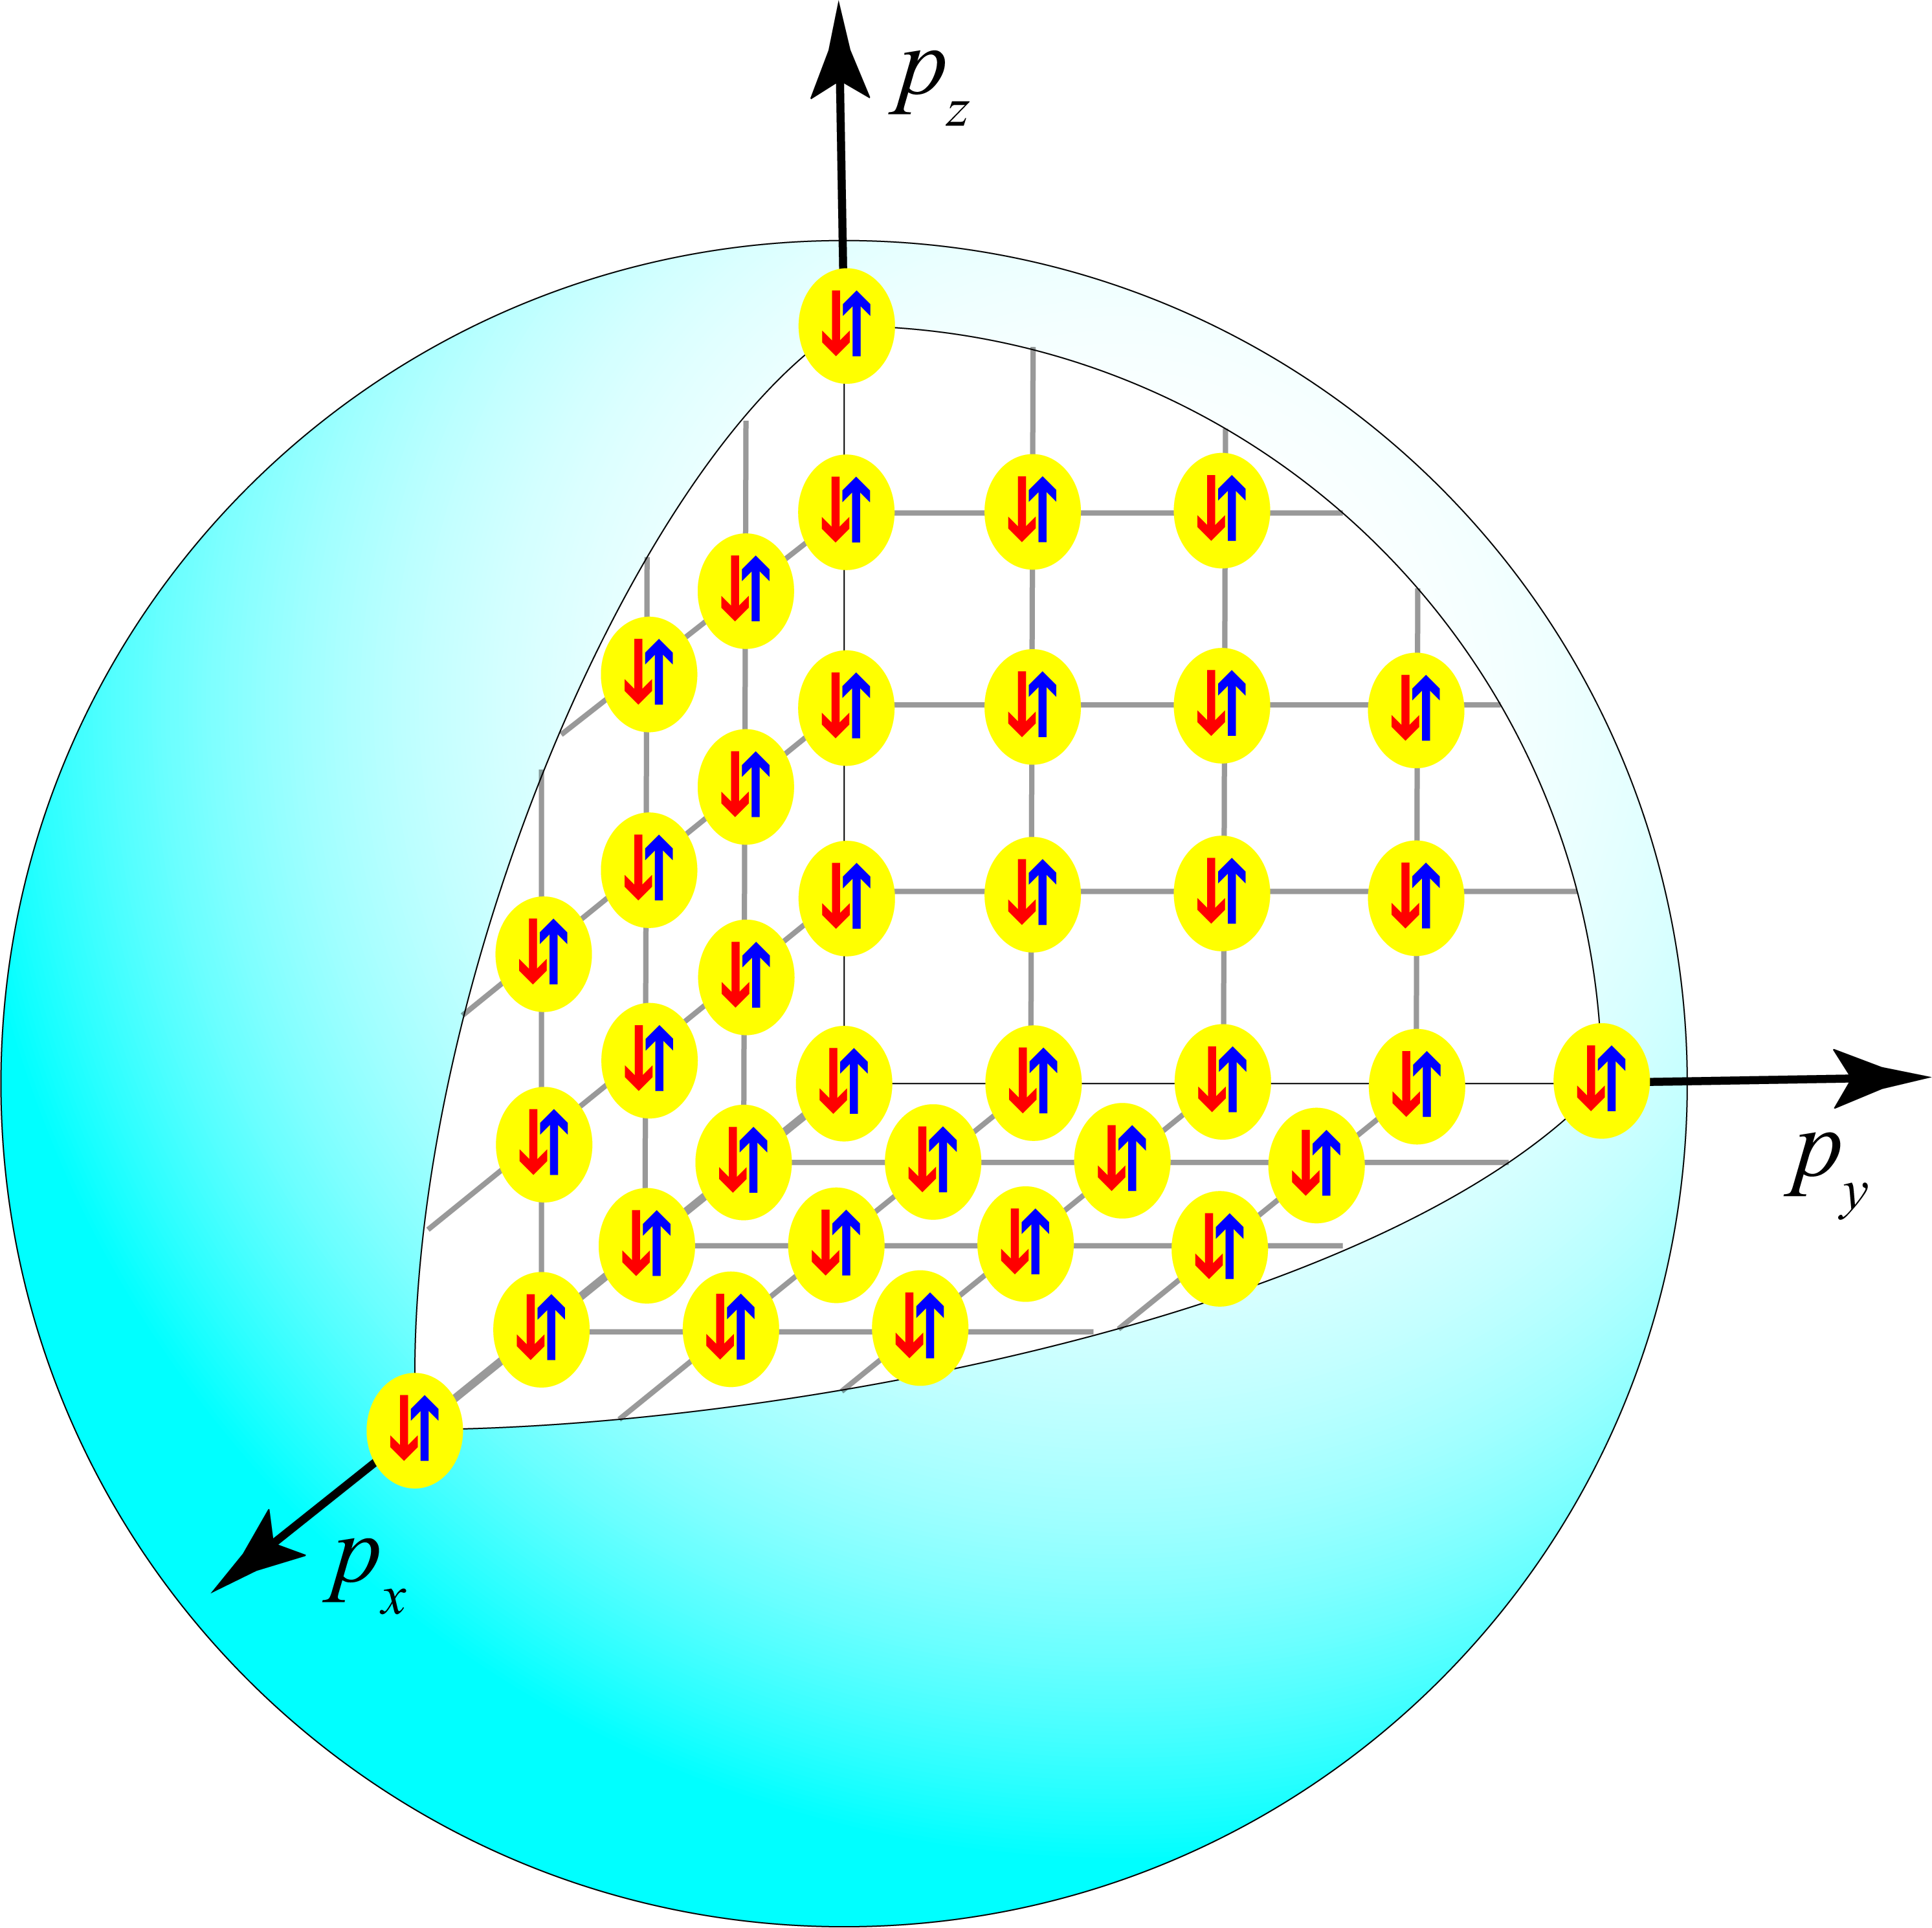
\includegraphics[width=7cm]{image/7-3-1.png}
\caption{电子态密度}
\end{wrapfigure}
现在把$N$个电子倒入动量空间中,\,那么电子在低温下将从最低能量态开始填充,\,由于电子数目巨大,\,最后电子将填充到能量为$\varepsilon_F$处.\,这样的一个填满电子的动量空间中的球体称为\emph{费米海}(fermi sea),\,最终填充到的能量称为费米能级$\varepsilon_F$,\,对应的电子动量为费米动量$p_F$.\,注意到一个动量空间中的一个标志状态的坐标内部实际上有两个独立的态,\,它们表示即使这两个波的波矢$\bs{k}$一样,\,它们代表电子的自旋也不一样\footnote{电子的微观描述是旋量波,\,也就是二分量波函数,\,具有两种可能的自旋.}.\,从而我们写出:
\[2\cdot\left.\frac{4\pi p_F^3}{3}\right/(\Delta p_x \Delta p_y \Delta p_z)=N\]

从而得到:
\[p_F=(\frac{3Nh^3}{8\pi N})^{\frac{1}{3}}=(\frac{3nh^3}{8\pi})^{\frac{1}{3}}\]

在以上过程中总电子数和总体积被消去了,\,最后电子堆积到的动量值仅仅取决于各处电子的数密度而成为了强度量.\,这样一个由于泡利不相容原理所造成的动量值对应到速度上,\,对一般金属估计约为$10^6\rm m/s$.\,而如果按非费米气计算,\,热运动速度应为$\sqrt{kT/m}\sim 7\pow{4}\rm m/s$,\,我们发现经典结果是严重估计少了的.\,但电子的热容又估计多了.\,量子统计给出:
\[c=\frac{\pi^2}{2}k\cdot\frac{kT}{\varepsilon_F}\]

代入热导率公式,\,得:
\[\frac{\kappa}{\sigma}=\frac{\pi^2}{6}\cdot\frac{mv_F^2}{\varepsilon_F}\cdot(\frac{k}{e})^2\cdot T\]

恰好,\,$\varepsilon_F=\dfrac{1}{2}mv_F^2$,\,从而我们得到了正确形式的魏德曼-弗朗茨定律:
\[\frac{\kappa}{\sigma T}=\frac{\pi^2}{3}(\frac{k}{e})^2\]

我们最后做一个经典德鲁特模型与量子费米气模型的比较.\,两个理论都承认以下基本公式的成立:
\[\sigma=\frac{ne^2 \tau}{m}\quad ,\quad \kappa=\frac{1}{3}nv^2\tau c\]

先看电导率,\,经典理论与量子理论对各个参数的估计除了$\tau$其他都是一致的.\,而经典更倾向于对$\tau$的估计更小.\,因为经典理论一般认为$\tau=\lambda/v$,\,而$\lambda$一般就按照原子实之间的平均距离来估计.\,这一点之后就知道是不妥当的,\,因为电子实际上可以在严格周期性的势能场中毫无散射的传播下去.\,而使得电子能够被散射的其实是晶格的缺陷,\,热振动等因素,\,从而一般温度升高,\,$\tau$减小,\,金属的导电性能就大大减弱.\,这给出了金属电阻随温度升高而升高的结论.\,这里经典理论对$\lambda$的过低估计恰好被对$v$的过低估计所抵消掉一部分,\,从而最后$\tau$的值在常温下差距也不大.\,而对于热导率,\,经典理论对$v$的过低估计又恰好被对$c$的过高估计修正,\,精确到了仅仅相差一个常数,\,除了经典理论说不清楚的$\tau$,\,经典与量子的在数量级上是基本符合的.

值得一提,\,热导率描述导热,\,电导率描述导电,\,而导电现象的附效应便是热产生.\,也就是\emph{焦耳热}(Joule heating).\,微观的功率密度
\[\bs{j}=\sigma \bs{E}\quad ,\quad w=\bs{j}\cdot\bs{E}\]

也即:
\[w=\sigma \bs{E}^2=\rho \bs{j}^2\]

其中\emph{电阻率}(resistivity)$\rho$为电导率的倒数.\,上为\emph{微观焦耳-楞次定律}(microscopic Joule-Lenz law).

\subsection{能带论*}

费米气模型在量子力学迅猛发展的几十年后回头看又是过于na\"\i ve了.\,人们发现电子终究是在晶格间传播的波动,\,如果原子实与背景的电子给出了严格的周期性的势能,\,那么如果电子的总机械能小于最大势能,\,那么就成为了束缚态,\,限制在一个原子附近运动而成为原子实的一部分.\,而如果电子守恒机械能大于最大势能,\,就成为不受任何阻碍的传导态.\,动能虽在运动中有所波动,\,但绝不会越来越小.\,描述电子的波函数称为\emph{布洛赫波函数}(Bloch wave function).\,而电子如何去填充怎样的能级?\,\emph{布洛赫}({\it F. Bloch})研究并发现了\emph{能带论}(energy band theory)来替代旧的费米气理论,\,这个理论可以统一地描述导体与绝缘体.

能带论可以看成是电子在单原子外的束缚态特征与传导的自由电子气的特征的一种综合,\,一方面电子在这样的一个周期性势场中的运动其守恒的机械能并不是可以取所有值,\,而是分为可以连续取值的区间:\,\emph{能带}(band)与根本取不到的能量区间:\,\emph{带隙}(gap)所构成.\,而电子作为波动用其所在的能带与波矢$\bs{k}$来描述.\,其波矢方向的物理意义不再重要,\,因为每一个态一般都代表某种驻波与行波的混合,\,而每一个态附近的群速度则可以代表这个态代表的真实电子运动速度.\,另一方面这些能带的结构又恰好对应到了单原子的束缚态能级.\,这使得我们经常是一望某元素的单原子核外电子排布,\,便能从其是否具有最外层电子读出这种元素单质是否能导电的信息.
\begin{figure}[H]
\centering
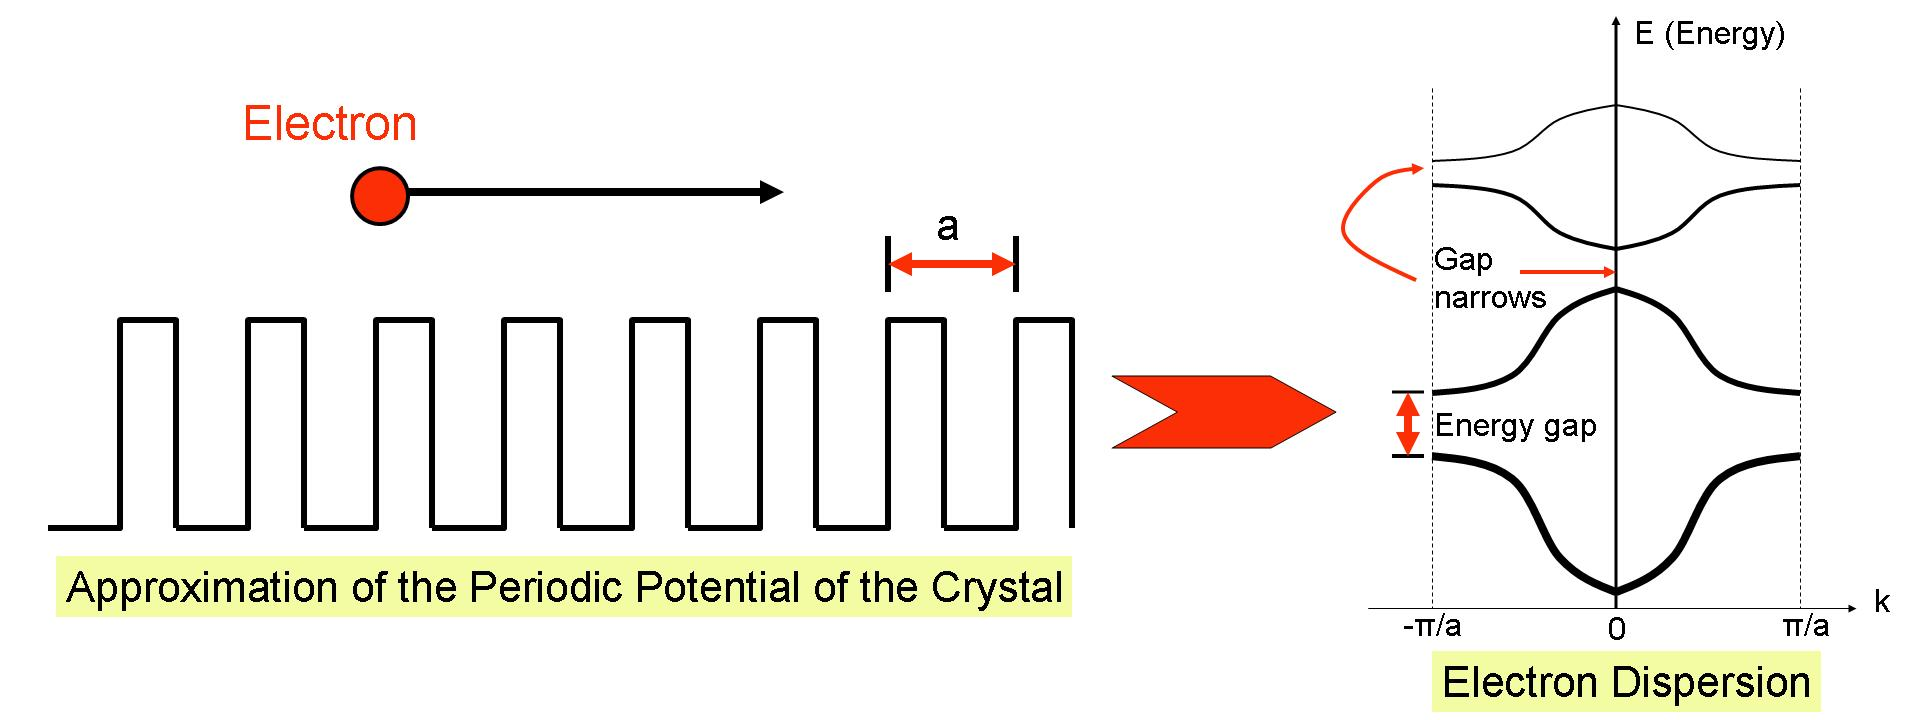
\includegraphics[width=0.8\textwidth]{image/7-3-2.jpg}
\caption{电子在周期性势场中传播}
\end{figure}

某种原子形成晶体时,\,电子从最低的能带开始填充,\,内层电子填满了较低的那些能带,\,它们不参与导电,\,对应于原子实电子和在晶体共价键键合的价电子.\,最外层电子较少的原子,\,形成晶体时最后填充的那个能带没有填满,\,或者虽然填满但与下一个能带在能量区间上重合而能够导电.\,称为\emph{导体}(conductor).\,对应的元素也就显示出明显的金属性\footnote{思考:\,氢是否具有金属性?\,参考\url{https://en.wikipedia.org/wiki/Metallic_hydrogen}.}.\,而若原子外层电子数目多,\,则很有可能电子恰好填满一个能带后隔着一个能隙与空的上方能带相望,\,则所有态都稳定不变,\,材料所有电子都是束缚电子,\,最后填充的那个满带称为\emph{价带}(valence band),\,代表原子间成共价键的价电子所在的能带.\,而上方的那个空带称为\emph{导带}(conduction gap).\,意为一旦这个带中存在电子则会大大改善其导电性能.\,此时元素体现出非金属性,\,一般形成的都是\emph{绝缘体}(insulator).\,而在金属性元素与非金属元素分界处则存在很多的\emph{类金属}(metalloid),\,它们形成的晶体虽然与绝缘体一样,\,在最低能量时恰好把价带排满,\,而隔着一个带隙与空的导带相望.\,但带隙很小(小于$4{\rm eV}$),\,导致常温的热激发和掺杂,\,抑或是光照激发都将在导带中激发大量载流子而具有可观的导电性能.\,这些材料称为\emph{半导体}(semiconductor).
\begin{figure}[H]
\centering
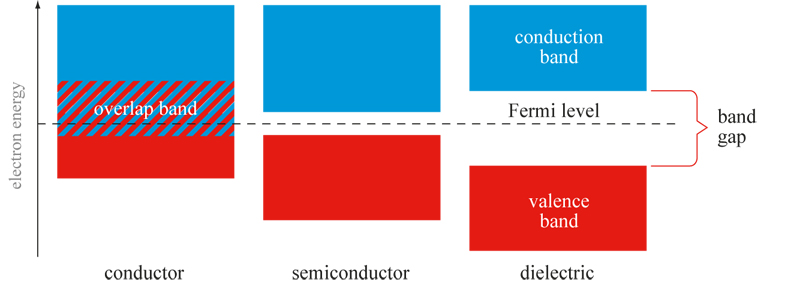
\includegraphics[width=0.8\textwidth]{image/7-3-3.jpg}
\caption{能带与导电性}
\end{figure}
\begin{figure}[H]
\centering
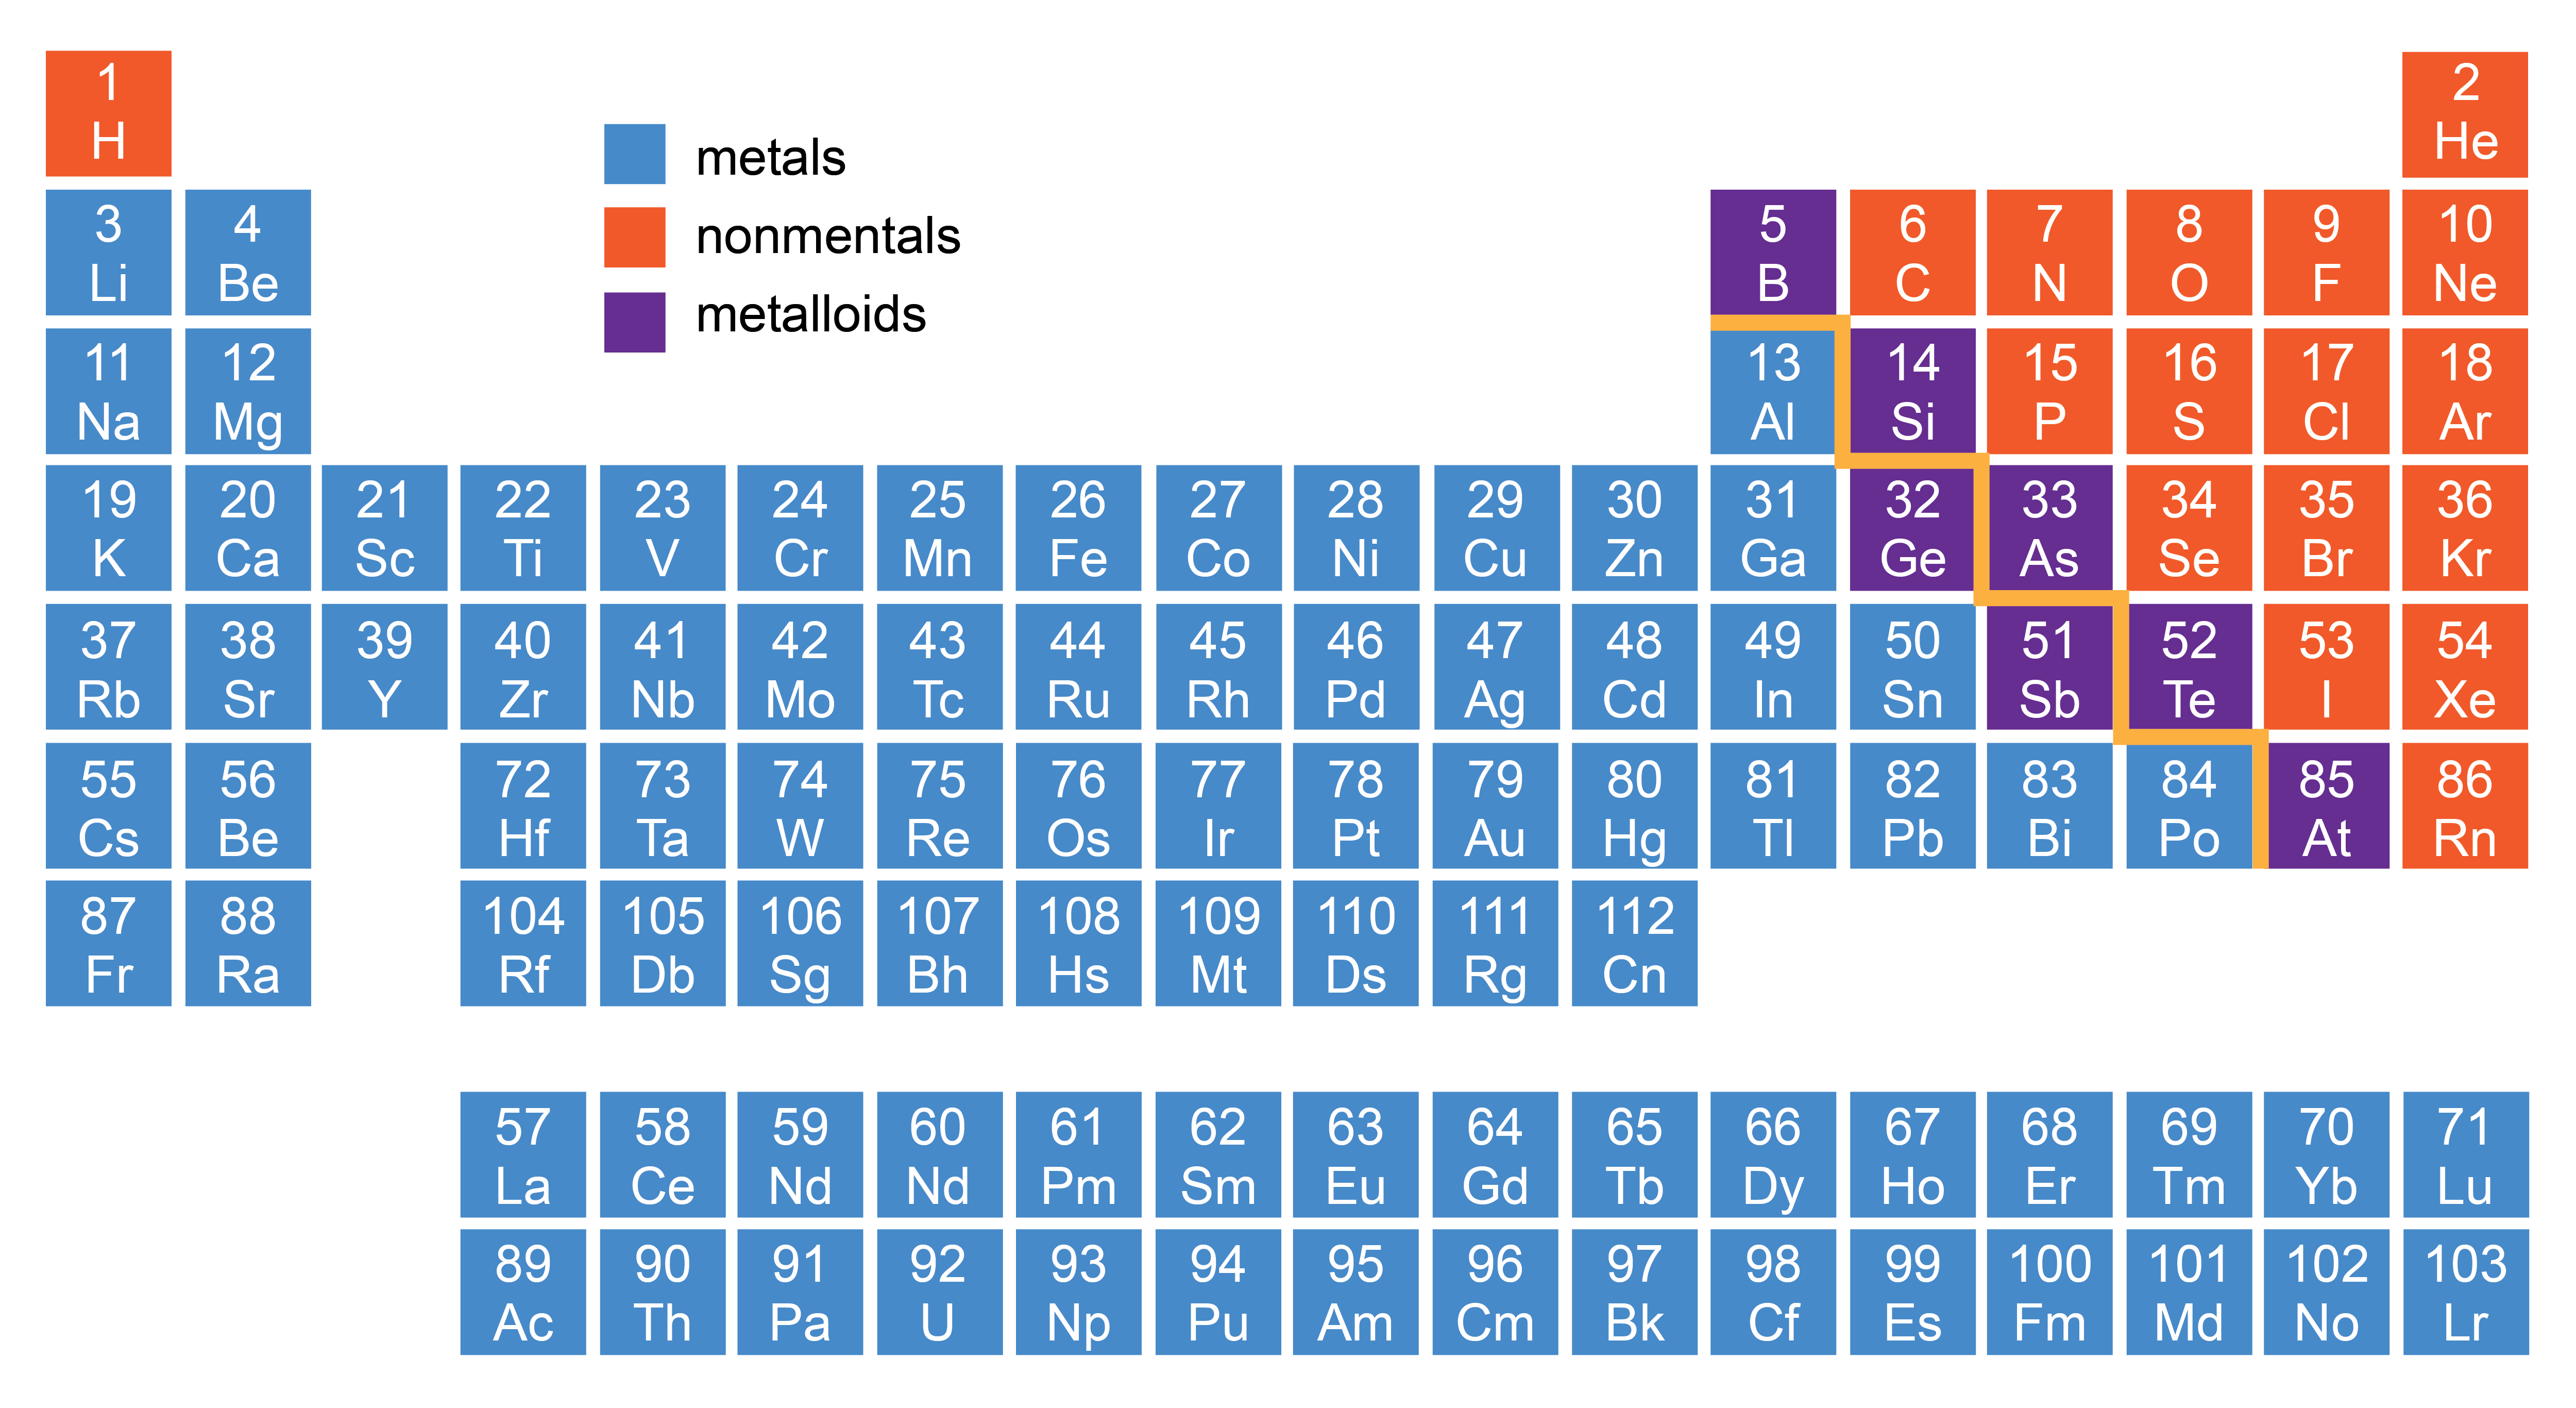
\includegraphics[width=0.8\textwidth]{image/7-3-4.jpg}
\caption{金属,\,类金属与非金属元素}
\end{figure}

那么能带论如何给出电导率的计算公式?\,仍然是:
\[\sigma=\frac{ne^2 \tau}{m}\]

与上一个费米气模型区别在于一点,\,就是这里的$m$不再是电子的\emph{裸质量}(bare mass),\,而是由于与周期性势场相互作用,\,电子的色散关系(能量与波矢关系)被修正后给出的\emph{有效质量}(effective mass).\,即使对于金属,\,这个质量与真实电子质量相差好几倍的现象也是十分普遍的.



\subsection{惯性,\,阻尼与回复力}

在量子力学还未诞生的时期,\,为了解释导体的导电,\,绝缘体的介电现象,\,并适用于任意交变电磁场在介质中的传播,\,色散,\,吸收与散射.\,洛伦兹提出著名的\emph{洛伦兹模型}(Lorentz model)作为德鲁特模型的补充.\,在这儿电子的惯性被重视,\,电子与晶格的碰撞被简化,\,可能的原子实对电荷的束缚被简化为线性回复你.\,也就是洛伦兹用唯象的谐振子类比来解释电子在外场下的行为:
\[m\ddot{\bs{r}}+\gamma \dot{\bs{r}}+ k\bs{r}=-e\bs{E}\ue^{i\omega t}\]

这个模型的解和它对应的各种特性我们将在光学教材里详细讲解.\,在这里我们仅仅讨论导体中的自由电子,\,故$k=0$.\,与导体导电相关的两个因素为:

一是阻尼系数$\gamma$.\,在直流电场下平衡时稳定的电子速度为:
\[\dot{\bs{r}}=-\frac{e}{\gamma}\bs{E}\]

对比更加本质的德鲁特等导电模型的电导公式,\,容易发现这个唯象系数与电导率和基本参量关系为:
\[\gamma=\frac{ne^2}{\sigma}=\frac{m}{\tau}\]

于是我们可以写出在导体上突然加一个不随时间变化的匀强电场后电子的运动的微分方程:
\[m\ddot{\bs{r}}+\frac{m}{\tau} \dot{\bs{r}}=-e\bs{E}\]

它的解为:
\[\dot{\bs{r}}=-\frac{e\bs{E}\tau}{m}(1-\ue^{-\frac{t}{\tau}})\]

我们十分自然地发现定义电子碰撞的弛豫时间恰好与导体对电场响应的弛豫时间相吻合.\,这一点稍微需要一些讨论和修正.\,见下.

第二点我们来讨论表示电子惯性的质量$m$.\,正是它导致了衰减因子$\ue^{-\gamma t/m}$,\,从而造成电路对电场响应的弛豫.\,但如果讨论电路的弛豫,\,或者说电流的惯性,\,有一点是被我们过低地估计了,\,便是自感现象.\,电荷的加速运动形成变化的电流,\,从而与之相伴的是变化的磁场.\,这个变化的磁场反过来给电流一个反向的作用力.\,由于该力正比于加速度,\,故等价于增加了载流子的质量.\,这里的弛豫时间对应直流暂态电路中的$\tau^\prime=L/R$.\,如果一定要理解为电子的惯性质量,\,那么一般比电子的裸质量要大好几个数量级$m^\ast\gg m$.\,从而一般有电路弛豫时间$\tau=m^\ast/\gamma$不等于微观碰撞弛豫时间.

纯粹的导体是否有回复力项?\,显然在以上电子运动方程中不含这一项.\,但注意到如果有回复力项,\,即使外场为零电子也会做振动.\,真实情况会发生这样的现象吗?\,答案是会,\,即\emph{等离子体振荡}(plasma oscillation).\,原因是电子相对于原子实的位移实际上在金属的表面累积了电荷分布,\,从而在内部激发了电场.\,由于频率很高,\,一般要到紫外波段的频率,\,我们可以完全忽略阻尼的影响.\,当电子有位移$\bs{r}$时将形成极化强度\footnote{显然此时``极化强度''描述的非极化电荷,\,而是自由电荷.}:
\[\bs{P}=-ne\bs{r}\]

我们考虑块状金属板\footnote{的确,\,取不同形状的物体这个频率会有所不同.}的集体等离子体振荡,\,那么由于金属表面的累积电荷在金属内部形成的电场为:
\[\bs{E}=\bs{E}_{\rm in}=-\frac{\bs{P}}{\varepsilon_0}=\frac{ne\bs{r}}{\varepsilon_0}\]

代入原方程:
\[m^\ast \ddot{\bs{r}}=-e\bs{E}=-\frac{ne^2\bs{r}}{\varepsilon_0}\]

从而得到谐振子方程.\,振荡频率为:
\[\omega_p=\sqrt{\frac{ne^2}{\varepsilon_0 m^\ast}} \quad;\quad\sigma=\varepsilon_0\omega_p^2\tau\]

最后我们考虑低频电磁波(内部实际场强)下金属的电子行为,\,利用光学中讨论过的洛伦兹模型,\,我们计算金属的复电容率,\,最后得到:
\[\varepsilon_r(\omega)=1-\frac{\omega_p^2\tau^2}{1+\omega^2\tau^2} \quad ; \quad \sigma(\omega)=\frac{\sigma}{1+\omega^2\tau^2}\]

一般$\omega_p\tau\gg 1$,\,故低频下金属的介电常数实际上是绝对值很大的负数.\,电导率随着频率的增加而减小.


\subsection{稳恒电流与形成条件}

作为电荷的流动,\,电流密度与电荷密度间满足电荷守恒定律:
\[\nabla\cdot\bs{j}+\frac{\partial\rho}{\partial t}=0\]

而所谓\emph{稳恒电流}(steady current)指的是一定区域内导电物质形成的电荷,\,电场,\,电流分布.\,其中电流的分布不能随时间变化,\,自然的结论是电荷密度分布也不能随时间变化.\,否则将产生随时间变化的电场,\,电场造成电流的变化.\,即上式必有:
\[\frac{\partial\rho}{\partial t}=0\quad;\quad \nabla\cdot\bs{j}=0\]

即在稳恒电流中电流密度是一定没有散度的,\,无头无尾的闭合曲线.\,稳恒电流必须是\emph{直流}(direct current)而非\emph{交流}(alternating current).

容易发现,\,在稳恒电流中微观欧姆定律写成以下形式是不完整的:
\[\bs{j}=\sigma \bs{E}\]

在很多情况下,\,上式并没有问题.\,$\bs{E}$被理解为由电荷分布$\rho$形成的静电场\footnote{实际上,\,不包括涡旋电场,\,因为它被归于之后引入的非静电力.\,换句话说,\,这里的$\bs{E}$不再由静止电荷的受力$\bs{F}/q$去定义,\,而是单纯根据静止电荷分布产生平方反比的电场叠加去定义.},\,它是一定可以引入电势的:
\[\bs{E}=-\nabla\varphi\]

\begin{wrapfigure}[13]{o}[-10pt]{8cm}
\centering
\vspace{-0.3cm}
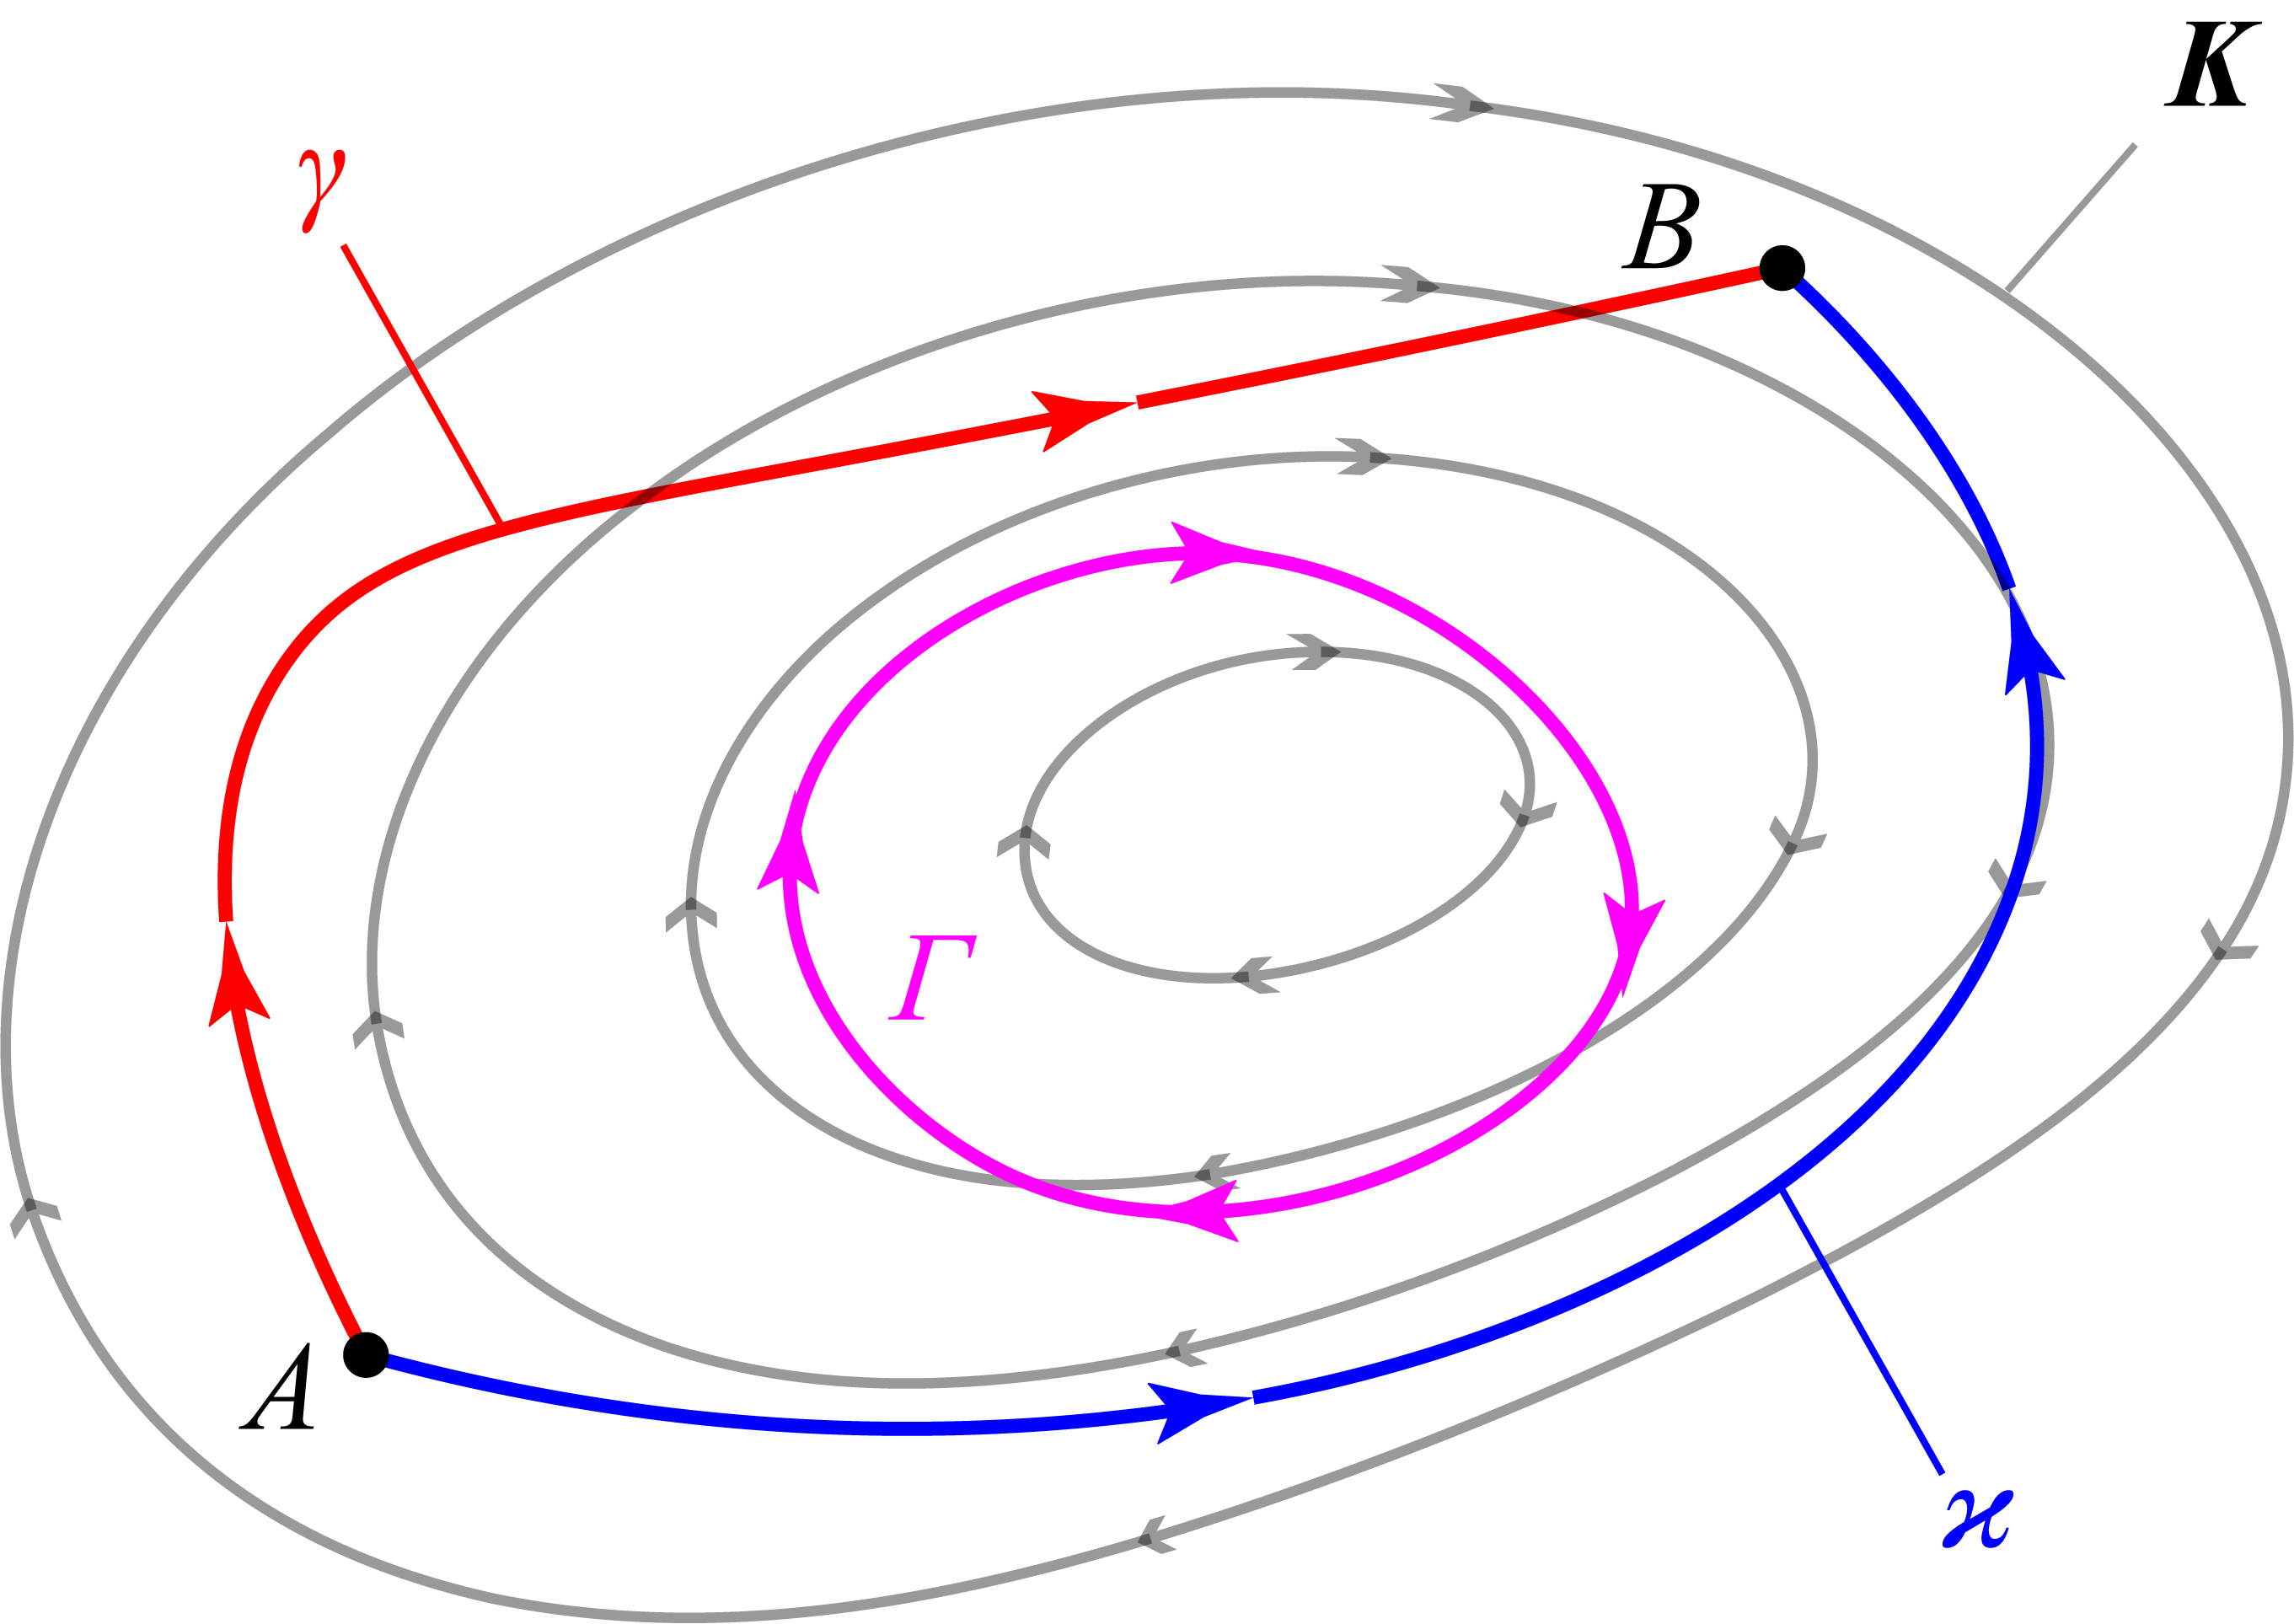
\includegraphics[width=8cm]{image/7-3-5.png}
\caption{非静电场}
\end{wrapfigure}
那么如果承认以上形式的微观欧姆定律就会引起矛盾:\,电流线是环状闭合的,\,电场线必须与电流线同向平行,\,但电场线又不能是闭合的,\,否则与静电场环路定理,\,电势的可定义性矛盾.\,实际上,\,微观形式的欧姆定律必须被写成:
\[\bs{j}=\sigma (\bs{E}+\bs{K})\]


上式$\bs{K}$代表\emph{非静电力场}(non-electrostatic field)对电子产生的作用.\,定义方式与电场量纲一致,\,都是单位正电荷的受力.\,这么写的不同之处就在于,\,把驱动电流的力分成了两部分:\,静电场$\bs{E}$是保守的,\,可以引入势的,\,在一个回路中不做功的,\,不吞吐能量的场(注意电流本身就会发热,\,这不是场造成的而是电荷定向流动碰撞晶格造成的).\,但非静电力就是源源不断做功驱动回路中电流流动的,\,非保守的,\,不能引入势来描述的场.\,虽然不能引入电势来描述非保守力,\,但可以用\emph{电动势}(electromotive force)来描述非静电力:
\[\mathscr{E}_\gamma=\int\limits_{A\stackrel{\gamma}{\longrightarrow}B} \bs{K}\cdot\ud\bs{r}\quad;\quad \mathscr{E}_\varGamma=\oint\limits_{\varGamma}\bs{K}\cdot\ud\bs{r}\]

不像对静电场的积分那样仅仅取决于端点,\,电动势与积分路径一一对应.\,回路电动势一般来说不为零,\,从而相同端点的两个路径电动势也不一定相等:
\[\mathscr{E}_\varGamma\neq 0\quad;\quad \mathscr{E}_\gamma\neq\mathscr{E}_\varkappa\]

非静电力既然能够作用在电子上,\,其形式一般就是电磁力,\,万有引力,\,或是惯性力.\,磁场力对应\emph{动生电动势}(motional emf),\,而由于变化的磁场激发的涡旋电场部分的电场力对应\emph{感生电动势}(transformer emf).\,电子会受到引力,\,1967年Schiff指出电子会因为引力的原因聚集到金属的底部.\,而后Dessler提出了严格的考虑晶格在重力场下压缩与不均匀情况下的电子平衡情况.\,引力是很弱的保守力,\,对金属内部电荷体系的影响虽然很小但绝不是不可观测.\,而与引力类似的惯性力则可以人工制造出很大的数值,\,而且可以使它非保守.\,试想加速旋转一个线圈,\,那么在随晶体加速的参考系里电子受到的角向惯性力就和受到一个电场力造成的效果没有本质的区别.

\begin{wrapfigure}[13]{o}[-10pt]{8cm}
\centering
\vspace{-0.5cm}
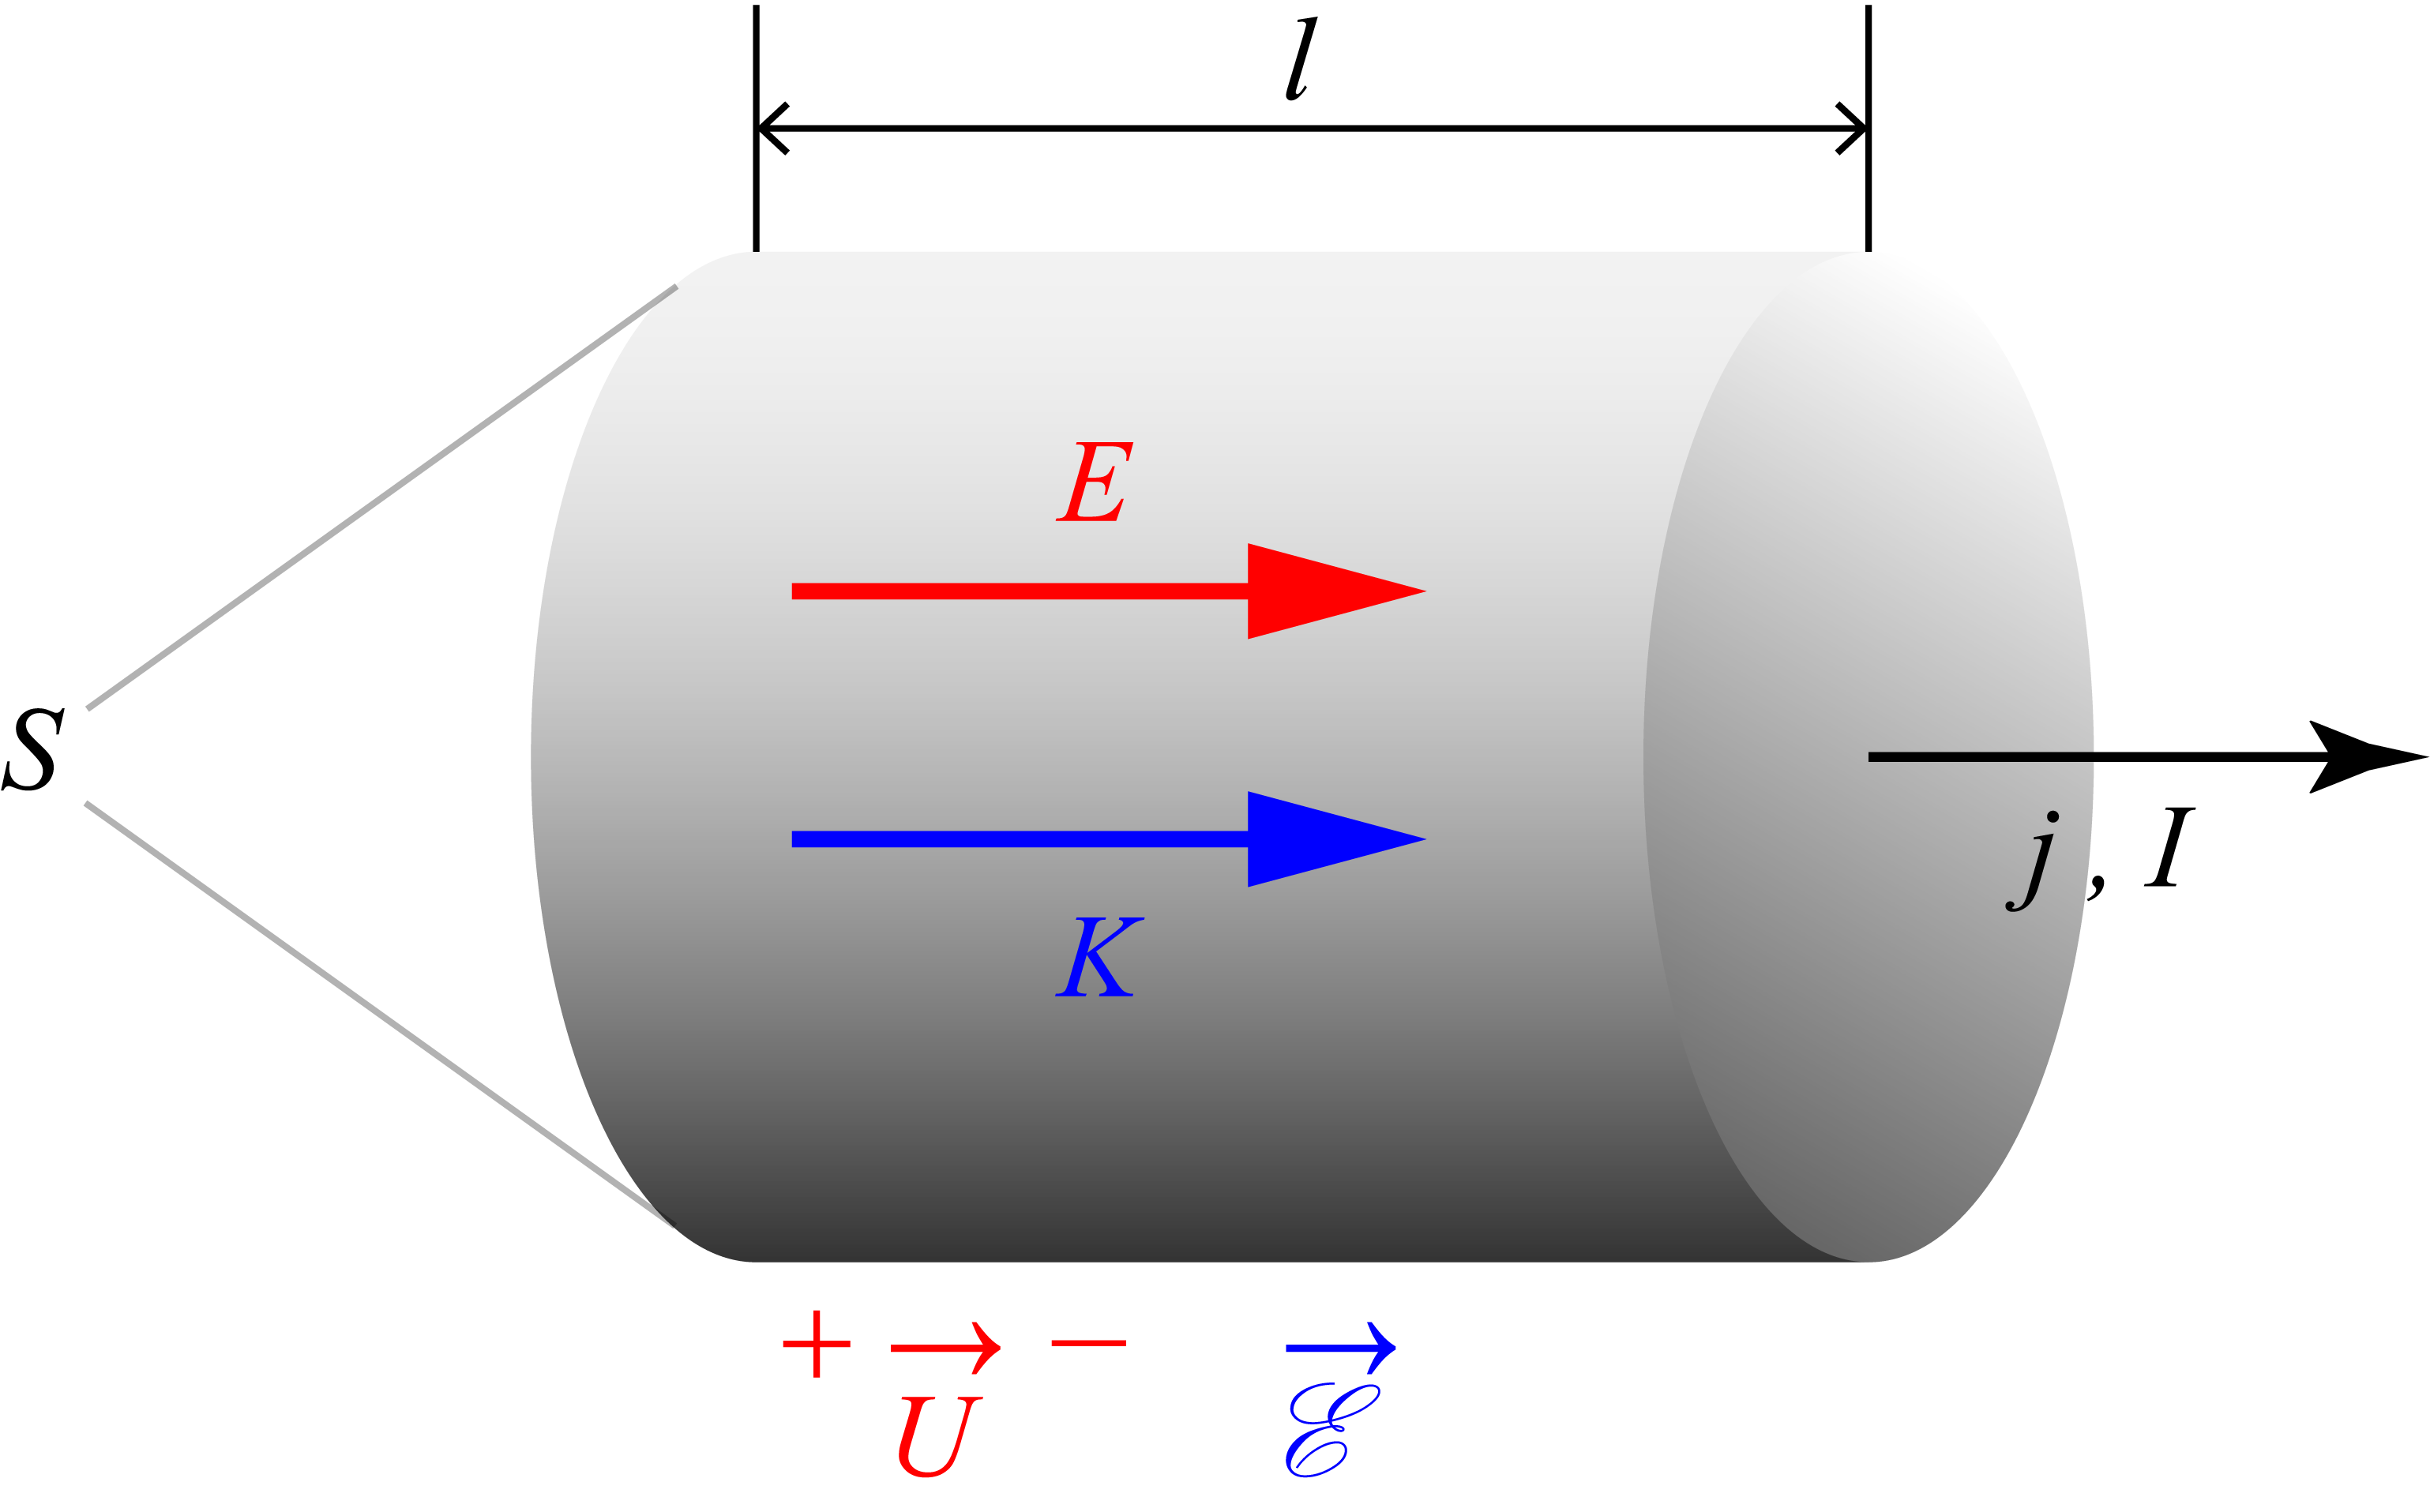
\includegraphics[width=8cm]{image/7-3-6.png}
\caption{宏观欧姆定律}
\end{wrapfigure}
还有一些电动势一般无法用非静电力描述.\,因为在一个回路中某些部分的确有能量的输入,\,但不是以作用在某些具体的电荷上的力的形式.\,而是更加广义的一些力作用在一些流上.\,例如温差电偶利用两种物质的电子的热扩散性质差异,\,从高温端吸取热量而驱动电流.\,化学反应更是源源不断地产生新的物质,\,利用反应的自发性而驱动物质做定向的移动形成电流.\,在这些抽象的场合,\,我们采用某段电路中移动单位电荷,\,外界向体系注入的能量来定义电动势:
\[\mathscr{E}=\frac{\ud W}{\ud Q}\]

\begin{figure}[H]
\centering
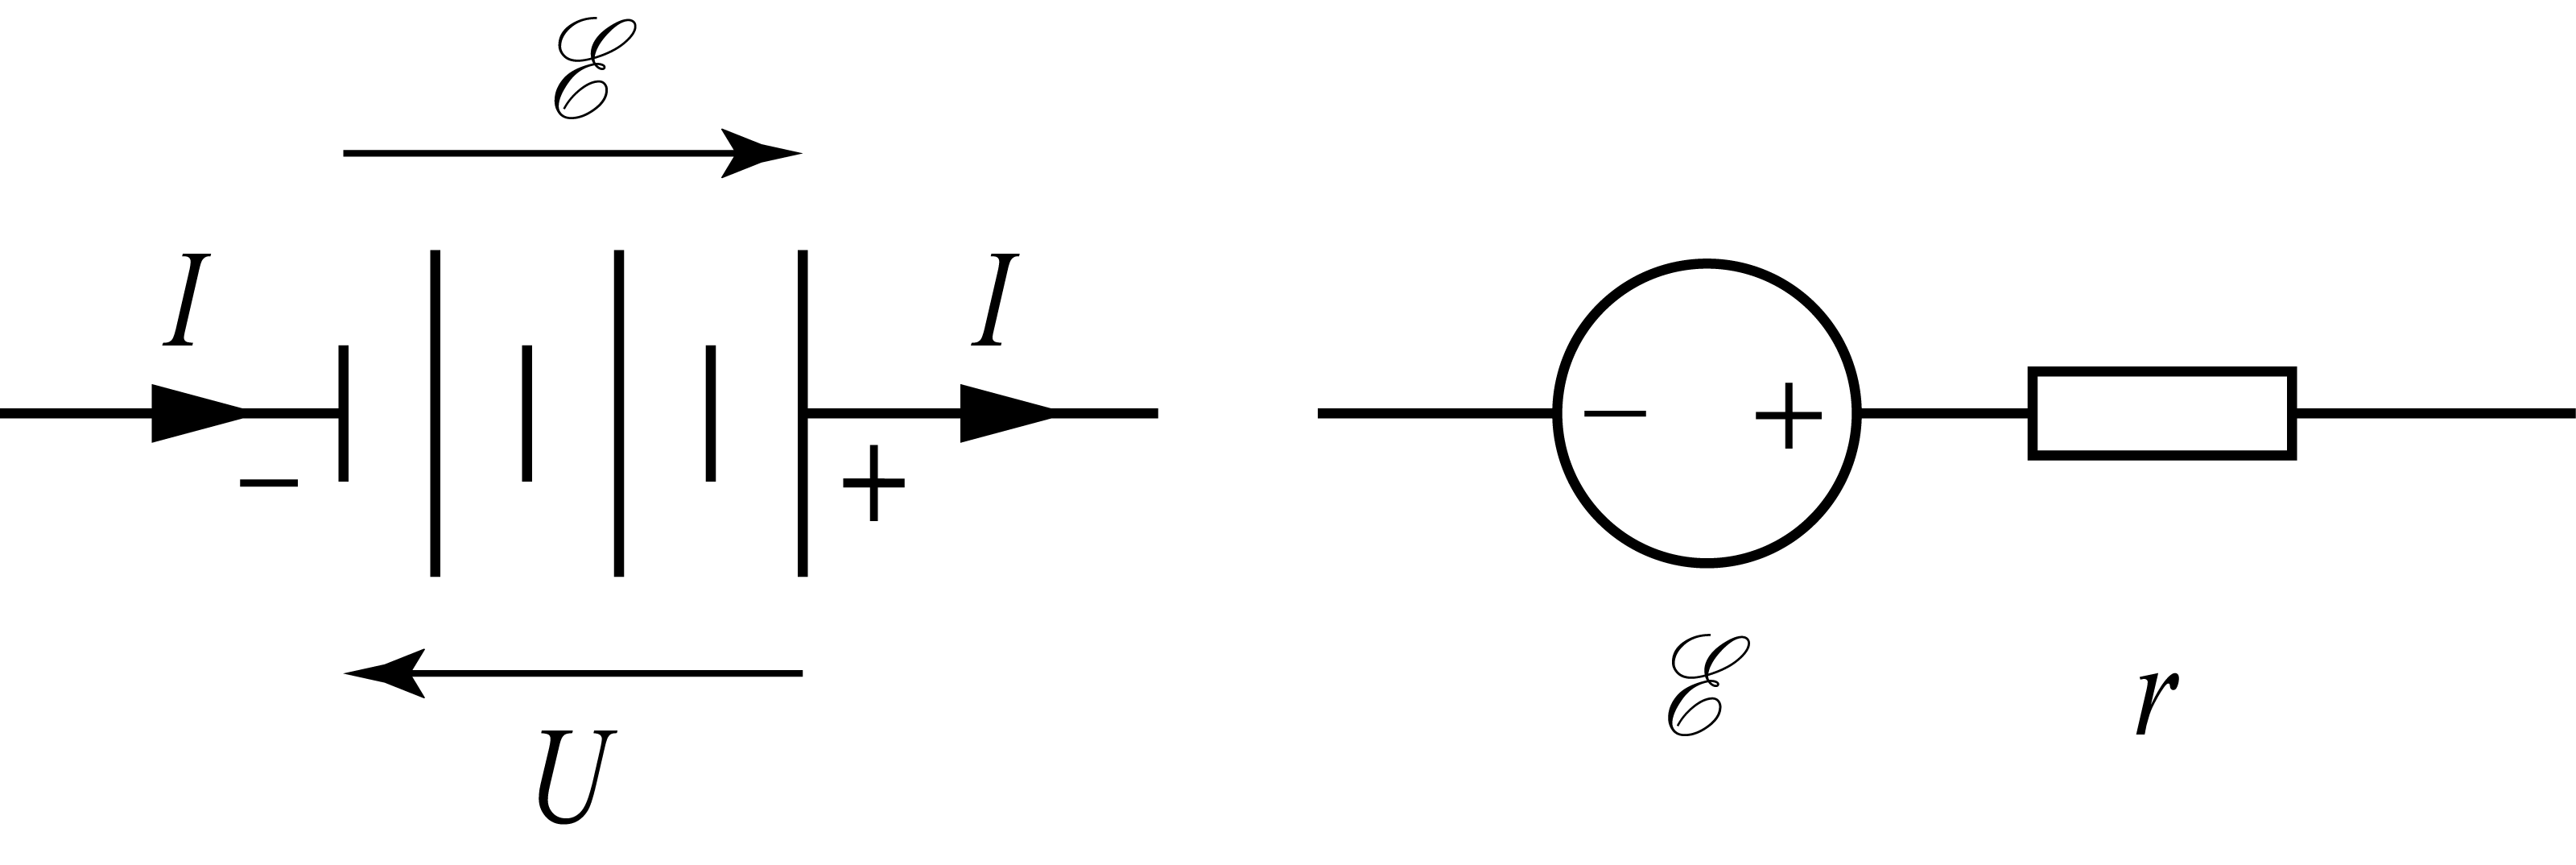
\includegraphics[width=0.6\textwidth]{image/7-3-7.png}
\caption{电池的欧姆定律}
\end{figure}
最后,\,从微观到宏观,\,我们考虑一段长为$l$,\,面积为$S$,\,电阻率为$\rho$的导体上的欧姆定律:
\[E+K=\rho j\]

等式两边同时乘以$l$,\,把电流密度写成$I/S$.\,得到:
\[U+\mathscr{E}=IR \quad;\quad R=\rho\frac{l}{S}\]

一般叫做部分电路的欧姆定律.\,而如果考虑\emph{电池}(battery)的两端,\,正常工作时一般正极电压更高,\,故约定电动势与电压取相反的方向,\,电流则与电动势方向一致,\,却与电压方向反向:
\[U=\mathscr{E}-Ir\]

为一段含源电路的欧姆定律.\,此时我们把电池等效为理想电压源和一个定值电阻$r$的串联.\,电阻即为电池的\emph{内阻}(internal resistance).






\section{电路与电路方程}

具体到直流电路中,\,我们一般提供以下理想的电路元件:
\begin{figure}[H]
\centering
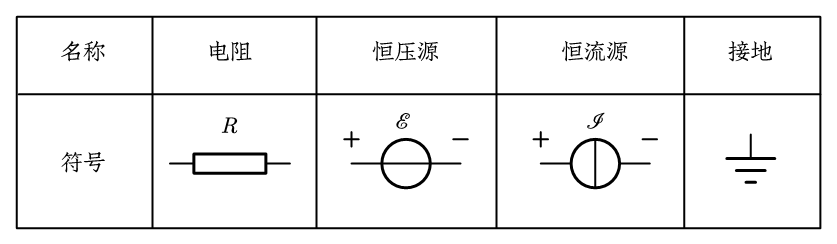
\includegraphics[width=0.7\textwidth]{image/7-3-8.png}
\caption{常见电路元件}
\end{figure}

实际电路总是由这些元件和导线构成,\,导线和元件的内阻均被用实际电阻显式表示.\,接地符号可以被视作特殊的导线.\,一般与真实的``地面''没有任何联系,\,电路中一般``地''指的是公共的零电势参考点.\,电路中如果仅仅有一个接地符号,\,就把接地的点的电势认为是零.\,如果出现了多个接地符号,\,就用导线把这些点连接到同一个点,\,并把这个点电势视作零.

\begin{wrapfigure}[12]{o}[-10pt]{8cm}
\centering
\vspace{-1cm}
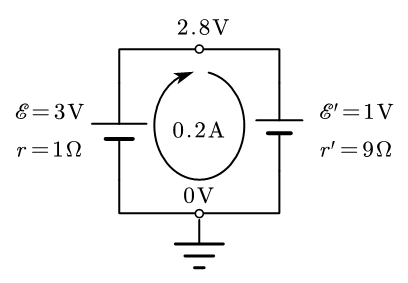
\includegraphics[width=8cm]{image/7-3-9.png}
\caption{相关方向}\label{fig7-3-9}
\end{wrapfigure}
任何一个元件,\,或者二端的部分电路,\,为了研究的统一性与方便,\,我们规定两端的电压的正方向与流过的电流的正方向都取``相关方向'',\,沿着这个方向,\,元件或部分电路表现的像一个电阻,\,或者宽泛一点说,\,像一个用电器.\,即电流就是沿这个方向流动,\,而且电压也沿这个方向降低.\,比如在如图\ref{fig7-3-9}所示的左侧大电池为右侧小电池充电的过程中,\,右侧电路对上下两端口以向下为电压电流的相关参考方向,\,则电压和电流分别为:
\[U=+2.8{\rm V}\quad ,\quad I=+0.2{\rm A}\]

但如果对左侧电路依然取向下为电压电流的相关参考方向,\,则电压和电流分别为:
\[U=+2.8{\rm V}\quad ,\quad I=-0.2{\rm A}\]

可以发现,\,如果一个元件或部分电路按照相关方向计算的电压电流同时是正或者负,\,这个元件就是\emph{类用电器}的,\,整体效果是消耗电能,\,而如果一正一负,\,就是\emph{类电源}的,\,整体效果是产生电能.

在具体分析复杂电路时,\,顺次串联的各个部分电路相关方向一般取为同向;\,讨论单个回路时,\,各个部分的相关方向也是按照某种环绕方向确定的;\,多个二端电路并联在两点之间也通常取各个支路为统一约定的从一个点到另一个点的相关方向.

对于之前的三种元件,\,电阻由于对称性没有天生的电压电流相关方向.\,无论如何取相关方向,\,其电压$U$,\,电流$I$和其参数电阻$R$都一定要满足:
\[U=IR\]

恒压源,\,顾名思义,\,总是能保持其正极电压比负极电压高$\mathscr{E}$.\,在正常工作状态时,\,电流应当从正极流出,\,使得其成为类电源的元件.\,取此时电流方向为其相关方向(具体问题中相关方向也可以与之相反),\,则其特性为:
\[U=-\mathscr{E}\quad ,\quad I>0\]

理想的恒压源同样能够工作在$I<0$的类用电器区域,\,此时同样有$U=-\mathscr{E}$.\,但是对理想电压源短路是没有意义的,\,一般恒压源所在支路一定需要串联电阻.

恒流源,\,顾名思义,\,总是能保持从负极向正极输出电流$\mathscr{I}$.\,在正常工作状态时,\,正极电压应当比负极电压高,\,使得其成为类电源的元件.\,取此时电流方向为其相关方向(具体问题中相关方向也可以与之相反),\,则其特性为:
\[I=\mathscr{I}\quad ,\quad U<0\]

理想的恒流源同样能够工作在$U>0$的类用电器区域,\,此时同样有$I=\mathscr{I}$.\,但是对理想电压源开是没有意义的,\,推广了看,\,一般恒流源所在支路一定需要并联电阻.

\section{电路分析基础}

\subsection{电路的整体结构与拓扑学结论}

\subsection{电路的求解套路}

\section{电路分析方法}

\subsection{二端电路等效}

\subsection{等效电阻计算方法}

\subsection{电路定理}

\section{半导体}

%!TEX root = ../physical-olympics-2.tex
\setcounter{chapter}{3}
\chapter{静磁场} 


\section{电流与磁场}

\subsection{磁场地位与电流分布}

\begin{itemize}
\item 磁场:\,运动电荷之间的相互作用.\,只有运动电荷才产生磁场,\,磁场也只对运动电荷造成力.

\item 但是运动与静止具有相对性,\,所以磁场是电场的相对论效应.\,即,\,如果认可一个参考系中电荷产生了磁场,\,那么就必须任何换一个参考系以后电荷也以另一种方式产生了相似的物质,\,但是如果变换到相对电荷静止的参考系,\,发现只存在电场,\,这就证明了磁场与电场描述的不过是同一种物质:\,\emph{电磁场}(electromagneto field).

\item 根据相对论的力变换公式:
\[F_x'=F_x-\frac{u}{c^2}\cdot\frac{v_yF_y+v_zF_z}{1-\frac{uv_x}{c^2}}\quad ,\quad F_y'=\frac{F_y}{\gamma (1-\frac{uv_x}{c^2})}\quad ,\quad F_z'=\frac{F_z}{\gamma (1-\frac{uv_x}{c^2})}\]

假设原参考系中只有电场,\,那么无论原参考系中的速度$v_x,\,v_y,\,v_z$如何,\,受力都不取决于速度大小,\,它是:
\[F_x=qE_x\quad ,\quad F_y=qE_y \quad ,\quad  F_z=qE_z\]

代入原式,\,并假设原参考系速度和变换速度相对$c$都是小量,\,故新参考系速度可以使用经典的速度叠加:
\[v_x=v_x'+u\quad ,\quad v_y=v_y' \quad ,\quad v_z=v_z'\]

近似到与$v_x',\,v_y',\,v_z'$一阶相关的领头项:

\[F_x'=qE_x-qv_y'\cdot \frac{uE_y}{c^2}-qv_z'\cdot \frac{uE_z}{c^2}\]
\[F_y'=qE_y+qv_x'\cdot \frac{uE_y}{c^2}\]
\[F_z'=qE_z+qv_x'\cdot \frac{uE_z}{c^2}\]

我们如果假设以下\emph{洛伦兹力}(Lorentz force)公式的成立性:
\[\bs{F}=q(\bs{E}+\bs{v}\times \bs{B})\]

事实上,\,这构成了磁场的严格定义,\,而且具有相对论协变性,\,这一点以后近代物理部分还会加以讨论.\,这个式子即:
\[F_x'=qE_x'+qv_y'B_z'-qv_z'B_y'\]
\[F_y'=qE_y'+qv_z'B_x'-qv_x'B_z'\]
\[F_z'=qE_z'+qv_x'B_y'-qv_y'B_x'\]

对比即知道:
\[B_x'=0\quad ,\quad B_y'=\frac{uE_z}{c^2} \quad ,\quad B_z'=-\frac{uE_x}{c^2}\]

这实际上是:
\[\bs{B}=-\frac{\bs{u}\times \bs{E}}{c^2}\]

如果原参考系是静止点电荷产生的电场,\,现在换参考系以后,\,点电荷做速度为$-\bs{u}$的匀速直线运动而产生以上磁场,\,那么就能推理出,\,如果点电荷以速度$\bs{v}$做匀速直线运动,\,那么它产生的磁场必然为:
\[\bs{B}=\frac{1}{4\pi \varepsilon_0 c^2}\frac{q\bs{v}\times \bs{e}_r}{r^2}\]

这其实就已经是毕奥-萨伐尔定律了,\,只不过历史上它是先通过\emph{奥斯特}(H. C. \O rsted)发现电流的磁效应,\,外加\emph{安培}(A. M. Amp\`ere)等人精妙设计的实验以实验规律给出,\,其形式略有变化,\,见下.\,表面上看推导出的毕奥-萨伐尔定律仅在低速下成立,\,但是麦克斯韦方程的协变性反过来证明了低速下它也是对的.

\item 本章讨论仅限于静磁场,\,即电流分布不随时间改变的磁场,\,上一节告诉我们这就是要求:
\[\nabla \cdot \bs{j}=0\]

\item 电荷运动,\,体电流元,\,面电流元,\,线电流元的等价性:
\[q\bs{v}\sim \bs{j}\ud V \sim \bs{i}\ud S\sim I\ud \bs{l}\]

\end{itemize}

\subsection{毕奥-萨伐尔定律}

\begin{itemize}
\item 电场与磁场的定义:\,任何情况下都是通过洛伦兹力公式:
\[\bs{F}=q(\bs{E}+\bs{v}\times \bs{B})\]

\item 磁场的国际单位:
\[1{\rm T}=10^4{\rm Gs}=1{\rm N/(A\cdot m)}\]

\item 实验规律:\,\emph{毕奥-萨伐尔定律}(Biot-Savart law):
\[\ud \bs{F}_{12}=I_2\ud \bs{l}_2\times \ud \bs{B}_{12}\quad ,\quad \ud \bs{B}_{12}=\frac{\mu_0}{4\pi}\frac{I_1\ud \bs{l}_1\times \bs{e}_{12}}{r^2}\]

虽然是实验规律,\,但之后的理论发展使得其中$\mu_0$不是新的常数,\,它直接被定义为:
\[\mu_0=\frac{1}{\varepsilon_0 c^2}=1.256637062\cdots \times10^{-6}{\rm H/m}\]

称作\emph{真空磁导率}(magnetic permeability of vacuum).
\end{itemize}


\section{两个定律与矢势}

\subsection{磁场环路定律}

\begin{itemize}

\item 磁场环路定律,\,又名安培环路定律:
\[\oint\limits_{\partial S}\bs{B}\cdot \ud \bs{l}=\mu_0 \int\limits_S\bs{j}\cdot \ud \bs{S}\]
\[\nabla\times \bs{B}=\mu_0 \bs{j}\]

\item 
\end{itemize}

\subsection{矢势与磁场高斯定律}

\begin{itemize}

\item 对电流元引入以下矢量场是方便的:
\[\bs{A}=\frac{\mu_0}{4\pi}\frac{\bs{j}\ud V}{r}\]

这是因为计算可得,\,这直接导致了:
\[\bs{B}=\frac{\mu_0}{4\pi}\frac{\bs{j}\ud V\times \bs{e}_r}{r^2}=\nabla\times \bs{A}\]

这个矢量称作\emph{磁矢势}(magnetic vector potential).

\item 由于叠加原理,\,一个电流分布体系的磁矢势和磁场应当为:
\[\bs{A}=\int\limits_V \frac{\mu_0}{4\pi}\frac{\bs{j}\ud V}{r}\quad ,\quad \bs{B}=\int\limits_V \frac{\mu_0}{4\pi}\frac{\bs{j}\ud V\times \bs{e}_r}{r^2}\]

同样地将满足:
\[\bs{B}=\nabla\times \bs{A}\]

\item 以上旋度关系写成积分形式意味着一种计算磁通量的特殊方法:
\[\Phi=\oint\limits_{\partial S} \bs{A}\cdot \ud \bs{l}=\int\limits_S\bs{B}\cdot \ud \bs{S}\]


\item 对于无边界的闭合曲面,\,上式直接证明了磁场高斯定律:
\[\oint\limits_{\partial V}\bs{B}\cdot \ud \bs{S}=0\]
\[\nabla\cdot \bs{B}=0\]

\item 可以设想存在可以像点电荷产生电场那样的方式产生磁场的物质,\,称作\emph{磁单极子`}(magnetic monopole),\,从而可以产生不为零的净\emph{磁荷}(magnetic charge),\,事实证明这样的物质至今都未曾找到,\,从而相伴的磁场形式也仅仅存在与理论中.\,但是,\,总磁荷为零的体系:\,\emph{磁偶极子}(magnetic dipole),\,不仅仅是纯粹的理论模型,\,后面可以发现线圈产生的磁场与磁偶极子是相似的.
\end{itemize}


\section{电流体系}

\subsection{磁偶极子}

\begin{itemize}
\item \emph{磁偶极子}(magnetic dipole)模型一般不指由正负磁单极子构成的体系,\,和电偶极子类似,\,它也来自矢势与磁场计算过程中的多极展开,\,由于需要用到较深的张量知识,\,在此仅仅给出展开的结果:
\[\bs{m}=\frac{1}{2}\int\limits_V \bs{r}\times \bs{j}\ud V\quad ,\quad \bs{A}=\frac{\mu_0}{4\pi}\frac{\bs{m}\times \bs{e}_r}{r^2}\quad ,\quad B_r=\frac{\mu_0}{4\pi}\frac{2m\cos\theta }{r^3}\quad ,\quad B_\theta=\frac{\mu_0}{4\pi}\frac{m\sin\theta }{r^3}\]

其中$\bs{m}$称作\emph{磁矩}(magnetic moment),\,任何情况下这都会是一个电流体系激发的磁场的领头项,\,因为磁单极子不存在,\,类似点电荷产生平方反比的电场那样的磁荷项,\,由于磁高斯定律,\,永远是不可能的.

\item 一个线圈,\,面矢量为$\bs{S}$,\,它的磁矩,\,由于以下积分公式:
\[\bs{S}=\frac{1}{2}\oint\limits_{\partial S}\bs{r}\times \ud \bs{r}\]

可以发现:
\[\bs{m}=\frac{1}{2}\int\limits_V \bs{r}\times I \ud \bs{l}=I\bs{S}\]

如果考虑$I\to \infty,\,S\to 0$的模型,\,就构成了\emph{点磁偶极子}(point dipole).

\item 磁偶极子的磁势能,\,受力与力矩:
\[V=-\bs{m}\cdot \bs{B}\quad ,\quad \bs{F}=\bs{m}\cdot \nabla\bs{B}\quad ,\quad \bs{M}=\bs{m}\times \bs{B}\]

\end{itemize}

\subsection{磁化强度}

\begin{itemize}
\item \emph{磁化强度}(magnetization):
\[\bs{M}=n\bs{m}\]

\item 磁化强度造成的体电流与面电流分布:
\[\bs{j}_M=\nabla\times \bs{M}\quad ,\quad \bs{i}_M=\bs{M}\times \bs{n}\]


\end{itemize}

\subsection{若干对称体系的磁场}

\begin{itemize}
\item 无限长载流直线:
\[\bs{A}=-\frac{\mu_0 I}{2\pi}\ln r\quad ,\quad \bs{B}=\frac{\mu_0 I}{2\pi r}\bs{e}_\varphi\]

\begin{figure}[H]
\centering
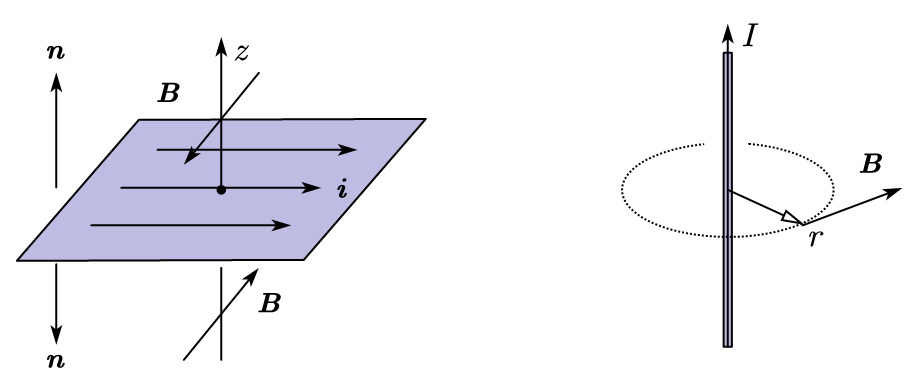
\includegraphics[width=0.7\textwidth]{image/7-4-1.png}
\caption{无限大平面与无限长直线}\label{fig7-4-1}
\end{figure}

\item 无限大载流平面:
\[\bs{B}=\frac{1}{2}\mu_0\bs{i}\times \bs{n}\]

\item 圆环:\,半径为$R$的标准载流线圈轴线上磁场:
\[\bs{B}=\frac{\mu_0IR}{2(R^2+z^2)^{\frac{3}{2}}}\bs{e}_z\]

该处的径向场强可以由磁高斯定理确定:
\[\frac{1}{2}\frac{\ud B_r}{\ud r}+\frac{\ud B_z}{\ud z}=0\quad \Rightarrow \quad B_r\approx -\frac{3\mu_0IRzr}{(R^2+z^2)^{\frac{5}{2}}}\]

\item 无限长密绕螺线管:\,无论其横截面形状,\,总是有:
\[B=\mu_0 i=\mu_0 nI=\frac{\mu_0 NI}{l}\]
\end{itemize}


\npg{-2cm}

\section{磁介质与磁能}

\subsection{微观角度理解磁化}

\begin{itemize}
\item 分子的固有磁矩:\,电子自旋磁矩+电子轨道磁矩.
\item 如果分子具有固有磁矩,\,那么按照热力学规律发生取向磁化:\,磁矩倾向于取与外磁场相同的方向,\,宏观上产生\emph{顺磁性}(paramagnetism).\,类似于电介质的极化,\,微观上顺磁磁化规律可以写作:
\[\bar{\bs{\mu}}=\alpha \bs{B}\]
\item 电子的磁矩与角动量的比称为\emph{旋磁比}(gyromagnetic ratio),\,轨道旋磁比与自旋旋磁比分别为:
\[\gamma_L=-\frac{e}{2m_e}\quad ,\quad \gamma_S=-\frac{e}{m_e}\]

角动量量子化理论告诉我们,\,$z$方向上电子轨道与自旋角动量只能为:
\[L_z=\pm n\hbar \quad ,\quad  S_z=\pm \frac{\hbar}{2}\]

故$z$方向上的磁矩的单位就是著名的\emph{玻尔磁子}(Bohr magneton):
\[\mu_B=\frac{e\hbar}{2m_e}=0.00579{\rm meV/T}\]

事实上由于自旋-轨道耦合,\,分子磁矩可以是玻尔磁子的分数倍.

\item 原子核也有磁矩,\,显然由于质子质量比质子质量大三个量级,\,故根据旋磁比算法,\,其磁矩也小三个量级.\,虽然对分子磁矩和宏观磁化几乎没有贡献,\,但是利用在磁场下形成的各个能级间跃迁吸收发射电磁辐射的原理可以造成\emph{核磁共振}(nuclear magnetic resonance)现象.

\item 如果分子的固有磁矩为零,\,那么在外磁场下会产生一个与外磁场反向的磁矩,\,宏观上造成\emph{抗磁性}(diamagnetism).\,从微观来看似乎与电介质极化的方向相反,\,但是从宏观效果上却与电介质削弱电场的效果相同,\,这是电与磁固有的区别导致的.

\item 抗磁性的微观起源为电子轨道运动的\emph{拉莫尔进动}(Larmor precession).\,由轨道运动产生的力矩,\,角动量,\,磁矩三者关系可得:
\[\bs{M}=\bs{\mu}\times \bs{B}\quad ,\quad  \bs{\mu}=\gamma \bs{L}\quad ,\quad  \frac{\ud}{\ud t}\bs{L}=\bs{M}\]
\[\Rightarrow \quad  \frac{\ud}{\ud t}\bs{L}=-\gamma \bs{B}\times \bs{L}=\frac{e\bs{B}}{2m}\times \bs{L}\]

故在运动学上,\,电子将以以下角速度发生进动:
\[\bs{\Omega}=\frac{e}{2m}\bs{B}\]

电子原来的轨道运动半径如果按照玻尔半径$a_0$估计,\,而角动量量级为$\hbar$,\,那么现在附加的角速度与原来的角速度的比为:
\[\Omega/\omega\sim\frac{ea_0^2}{2\hbar}B\]

故产生的磁矩与原来的玻尔磁子的比值的量级也与之相当,\,得到磁矩的量级为:
\[\bar{\bs{\mu}}\sim-\frac{e^2a_0^2	}{4m}\bs{B}\]

系数便是抗磁性磁化的分子磁化率的量级,\,它一般比顺磁性磁化要小一到两个量级.

\item 有一些金属,\,或者特殊的金属化合物具有独特的\emph{铁磁性}(ferromagnetism),\,微观上它们由介观的包含大量原子的\emph{磁畴}(magnetic domains)构成.\,每一个磁畴由于单元之间的关联已经超过了热力学的涨落而成为了决定性的因素,\,使得所有电子的自旋几乎都严格指向同一个方向,\,磁化达到饱和.\,而材料的磁化过程其实是不同的磁畴在外磁场下的转向.\,它的磁化率将远远大于简单的顺磁和抗磁磁化.\,而且体现出非线性和历史相关性.


\end{itemize}

\subsection{宏观角度理解磁化}

\begin{itemize}
\item 出于$\bs{B}$和$\bs{M}$的旋度分别为总电流密度和磁化电流密度,\,引入\emph{磁场强度}(magnetic field strength)以区别于以往一贯描述磁场的$\bs{B}$,\,一般可区别称作\emph{磁通密度}(magnetic flux density):
\[\bs{H}=\frac{\bs{B}}{\mu_0}-\bs{M}\]

这样这个矢量的旋度就只取决于外电流:
\[\nabla\times \bs{H}=\bs{j}_f\]

\item 在顺磁或铁磁的柱状介质外绕制密绕螺线管,\,那么没有介质时其磁通密度为:
\[B_0=\mu_0 i\]

那么,\,由于此时加入介质时磁化电流不影响$\bs{H}$的计算,\,故磁场强度为:
\[H=\frac{B_0}{\mu_0}=i\]

但是磁化电流的存在将产生一个与原磁场同向的附加磁场,\,使得介质内部的磁场变大,\,那么定义此时磁场与原磁场的比值为\emph{相对磁导率}(relative magnetic permeability):
\[B/B_0=\mu_r\]

那么把绝对磁导率定义为$\mu=\mu_r\mu_0$,\,就有以下关系式:
\[B=\mu H=\mu i\]

\[M=(\mu_r-1)H=\chi_m H\]

其中$\chi_m$就是宏观的\emph{磁化率}(magnetic susceptibility).\,对于抗磁性物质,\,其值是小于零的.


\end{itemize}

\subsection{磁场能量}

磁场体系的能量的计算方法可以证明可以有用电流与矢势和用能量密度两种计算方法:
\[I=\frac{1}{2}\int \bs{j}\cdot\bs{A}\ud V=\int \frac{1}{2\mu_0}	\bs{B}^2\ud V\]

同样地,\,两个体系同时存在时,\,体系将产生自能与相互作用能.\,如两个电感元件如果之间存在互感,\,那么其总能量应当为:
\[E=\frac{1}{2}L_1I_1^2+\frac{1}{2}L_2I_2^2+ MI_1I_2\]

如果存在介质,\,其能量密度需要加上磁化带来的能量,\,能量密度变为:
\[w=\frac{1}{2\mu}	\bs{B}^2=\frac{1}{2}\mu \bs{H}^2 =\frac{1}{2}	\bs{B}\cdot \bs{H}\]

%\section{超导简介}

%!TEX root = ../physical-olympics-2.tex
\chapter{电磁感应}


\section{动生电动势}
\begin{itemize}
\item 动生电动势的非静电力:\,磁场力沿导线方向的分量:
\[\bs{K}=\bs{v}\times \bs{B}\]

\item 回路的总动生电动势的计算方法:
\[\mathscr{E}_m=\oint \bs{K}\cdot\ud \bs{l}=-\left.\frac{\ud \Phi}{\ud t}\right|_{B\text{不变}}\]

总电动势等于磁通量变化率,\,这就是法拉第电磁感应定律的动生部分.

\item 一段电路动生电动势做功的功率:
\[\ud P_{\mathscr{E}}=\ud \mathscr{E}\cdot I=I(\bs{v}\times \bs{B})\cdot \ud\bs{l}\]

该功率变成了电路内部的能量.\,但是注意到磁场力的另外一个分力:\,安培力也要做功,\,功率为:
\[\ud P_A=\ud \bs{F}\cdot \bs{v}=I(\ud\bs{l}\times \bs{B})\cdot  \bs{v}\]

这个功将转化为导线的机械能.\,那么由于磁场力本质上不会做功,\,这一点很容易就能够利用三重标积公式在两个功率上得到印证:
\[\ud P_{\mathscr{E}}+\ud P_A=0\]

从而两个功率的大小代表机械能和电能转化的快慢.\,对于电动机,\,电能转化为机械能,\,对于发电机,\,机械能转化为电能.
\end{itemize}

\section{感生电动势}

\begin{itemize}
\item 相对性原理容易说明,\,如果产生磁场的物质在发生运动以致使其发生变化,\,那么即使线圈静止,\,也会产生感应电动势.\,那么内部电荷受到的非静电力就必然不是磁场力,\,因为根据电磁场的定义:
\[\bs{F}=q(\bs{E}+\bs{v}\times\bs{B})\]

而现在线圈$\bs{v}=\bs{0}$.\,我们只能把这个力称作电场力.\,这种电场称作\emph{感生电场}(induced electric field).\,它可以理解为由变化的磁场产生的.\,事实上,\,磁场又由电流产生.\,故可以直接认为这个感生电场就是由变化的电流产生的.\,更有甚者,\,以下关系式均是成立的:
\item 感生电场公式:
\[\bs{E}=-\frac{\partial \bs{A}}{\partial t}=-\int \frac{\mu_0}{4\pi}\frac{\frac{\partial \bs{j}}{\partial t}}{r^2}\ud V\]

\item 将上式对回路进行积分便得到感生电动势:
\[\mathscr{E}_i=\oint \bs{E}\cdot\ud \bs{l}=-\frac{\partial }{\partial t}\oint \bs{A}\cdot \ud \bs{l}=-\frac{\partial \Phi}{\partial t}=-\left.\frac{\ud \Phi}{\ud t}\right|_{S\text{不变}}\]

这就是法拉第电磁感应定律的感生部分.

\item 将感应电动势的动生和感生部分合并,\,得到完整的法拉第电磁感应定律:
\[\mathscr{E}=-\frac{\ud \Phi}{\ud t}\]

\end{itemize}

\section{自感与互感}

\begin{itemize}
\item 自感定义与自感系数公式:
\[\Psi=LI\quad ,\quad L=\frac{\mu N^2 S}{l}\]

\item 两线圈互感时的相关公式:
\[E=\frac{1}{2}L_1I_1^2+\frac{1}{2}L_2I_2^2+ MI_1I_2\]

\[\Psi_1=L_1I_1+MI_2\quad \Rightarrow\quad  U_1=-L_1\frac{\ud I_1}{\ud t}-M\frac{\ud I_2}{\ud t}\]
\[\Psi_2=L_2I_2+MI_1\quad \Rightarrow\quad  U_2=-L_2\frac{\ud I_2}{\ud t}-M\frac{\ud I_1}{\ud t}\]
\[U_1I_1+U_2I_2=-\frac{\ud E}{\ud t}\]
\end{itemize}


%!TEX root = ../physical-olympics-2.tex
\chapter{统计物理基础}

\section{数学基础}


\subsection{概率与独立性}
现实生活中有很多偶然事件,\,偶然事件的成因是多种多样的,\,它们集中表现在相似的条件下进行试验,\,而能够得到完全不同的结果.\,数学上用抽象的集合来表示所有可能的结果:
\[x\in X,\quad X=\{x\}\]

其中每一个元素代表一种可能的结果.\,这些结果应该有以下特点:
\begin{quote}
{\hei 忠实性}:\,每一个不同的实验结果如实地反应为集合中的不同元素.\,也就是不能用一个元素代替一类实验结果.\\
{\hei 互斥性}:\,当一个结果发生时,\,另一个结果就必须排除,\,也就是不能有多个元素对应同样的实验结果.\\
{\hei 完备性}:\,所有的实验结果必须都有集合中的元素对应.
\end{quote}

这样就能把集合\(X\)称为\emph{样本空间}(sample space),\,而每一个元素\(x\)也称为一个\emph{元事件}(elementary event).\,我们常说的\emph{事件}(event),\,其实一般指样本空间的一些定义良好的子集\(A\subset X\).\,只要实验结果在这个子集中,\,就说这个事件发生了.\,所谓定义良好我们可以做如下理解:

在\emph{古典概型}(classic models)情形下,\,样本空间是一个有限的集合,\,此时任意子集都可以视为某种事件.\,如投一颗骰子,\,样本空间为\(X=\{1,2,3,4,5,6\}\),\,则投出偶数是一个事件\(A=\{2,4,6\}\).

但在\emph{几何概型}(geometric models)情形下,\,样本空间一般具有与\(\mathbb{R}^n\)类似的结构,\,一般都是无限的集合,\,有一些``事件''的提法应当给予摒弃否则会引起矛盾.\,例如在闭区间\([0,1]\)间任取一个点,\,这个点恰好是有理数这样的``事件''可能就不是那么定义良好\footnote{事实上有理数集是定义良好---可测的,\,但有些集合不可测从而不能讨论它们的概率.\,参考\url{https://en.wikipedia.org/wiki/Non-measurable_set}}.\,一般常见的事件如点落在区间\((a,b)\)内等等.

设想同时做好几个实验,\,这几个实验互不干扰\,它们的结果是完全独立的,\,那么联合到一起就构成了一个大的实验,\,其结果应表示为一个数组:
\[\bs{x}=(x_i)\quad ;\quad x_i\in X_i\]

而新的样本空间称为原来那些样本空间的\emph{独立直积}(independent product).\,记做:
\[\bigotimes_i X_i=\{\bs{x}=(x_{ij})|x_{ij}\in X_i\}\]

互斥,\,独立这样的一些概念如何用数学严格表述?\,事实上它们恰恰是用概率去定义的.\,概率是一种我们关于实验结果可能性的\emph{先验假设}(a priori presumption),\,它是\emph{随机变量}(random variable)的正实数值函数\(P\),\,而随机变量既可以取为样本空间中的单个结果,\,也可以取为结果的集合:\,事件:
\[P(A)=P(\bigcup_{x_i\in A} {x_i})=\sum_{x_i\in A} P(x_i)\]

这其中已用到了\(P\)的属性:\,\emph{互斥事件}(mutual-exclusive events, disjoint events)的加法原理:
\[A\cap B=\emptyset\quad \Rightarrow\quad P(A\cup B)=P(A)+P(B)\]

再加上:
\[P(A)\geqslant 0\quad ;\quad P(X)=1\]

就构成了一个合适的概率定义.\,而对于随机变量可取连续样本空间,\,比如区间\([a,b]\)的情形,\,引入\emph{概率密度函数}(probability density function, pdf):
\[P([x,x+\ud x])=p(x)\ud x\quad ;\quad p(x)>0\;,\;\int_a^b p(x)\ud x=1\]

便是一个合适的概率定义.

现在来讨论事件的独立性.\,两个非互斥的事件可能同时发生,\,同时发生这一个新的事件即被定义为\(A\cap B\neq \emptyset\),\,此时可以定义事件\(B\)在事件\(A\)下的\emph{条件概率}(conditional probability):
\[P(B|A)=\frac{P(A\cap B)}{P(A)}\]

显然,\,若条件概率为零,\,那么实际上两个事件互斥.\,而实际上如果\(B\)在\(A\)下的条件概率等于\(B\)的概率,\,那么这种情况称为两个事件相互独立:
\[P(B|A)=P(B)\]

注意到上式实际上也可以写为:
\[P(X)P(A\cap B)=P(A)P(B)\]

所以两个事件相互独立的确是一个相互的关系,\,此时\(A\)的条件概率也有\(P(A|B)=P(A)\).\,两个事件相互独立是一种很微妙的关系,\,这意味着一个事件的发生既不会阻碍另一个事件,\,也不会促成另一个事件.\,而是完全没有影响.\,物理上看,\,很有可能两个事件没有因果关系.

我们之前构造的独立直积,\,用概率表示即为:
\[P((x_{ij}))=\prod_i P(x_{ij})\]

而对于连续概率分布,\,两个样本空间的独立直积给出的新概率应该是有以下概率密度:
\[p(x,y)=p_1(x)p_2(y)\]

\subsection{随机变量及其数字特征}
物理实验中的随机现象,\,常常体现为实验测量中测量结果数据的上下波动.\,此时一般认为这个测量数据\(x\)就是一个随机变量,\,而具有先验的某种概率密度函数\(p(x)\).\,.\,有时候我们关心测量数据的某种函数\(y=f(x)\),\,那么不同的\(y\)其出现概率分布应该修改:
\[p_y(y)=\frac{\ud p}{\ud y}=\frac{p(x)\ud x}{\ud y}=\frac{1}{f'}p(x)\]

例如,\,如果考虑在\(x\)方向的粒子速度\(v\)具有分布律:
\[p(v)=\frac{1}{\sqrt{2\pi}}\ue^{-\frac{v^2}{2}}\]

可以验证这个概率归一,\,那么其能量\(e=\dfrac{v^2}{2}\)的分布为
\[p_{e+}=\frac{p(v)}{v}=\frac{1}{2\sqrt{\pi e}}\ue^{-e}(v>0)\quad ;\quad p_{e-}=\frac{p(v)}{-v}=\frac{1}{2\sqrt{\pi e}}\ue^{-e}(v<0)\]

注意到同一个能量对应着两种可能的运动方向,\,故把两个\(\ud e\)对应概率分开算,\,最后合到一起:
\[p_e(e)=\frac{1}{\sqrt{\pi e}}\ue^{-e}\]

一个在统计中关心的数学处理,\,是在\(n\)次全同独立测量中获得的测量结果的\emph{平均数}(average):
\[\bar{x}=\frac{x_1+x_2+\cdots+x_n}{n}\]

而著名的\emph{大数定律}(law of large numbers)指出:\,如果概率分布的一个重要数字特征:\,\emph{期望}(expectation)存在\footnote{值得指出,\,有些数学上诡异的概率分布是不存在期望的,\,比如典型的柯西分布:
\[p(x)=\frac{\gamma/\pi}{x^2+\gamma^2}\]

当然这样的理想概率分布物理上几乎不存在,\,因为物理量总是有限的,\,在一定尺度下适用.}:
\[\mu=\langle x\rangle=\int x\ud p\]

那么如果随着测量次数趋于无穷,\,平均数将会无限趋近于期望值:
\[\lim_{n\to \infty}P(|\bar{x}-\langle x\rangle|>\varepsilon)=0\; , \; \forall \varepsilon>0\]

如何理解这一点?\,我们再定义另一个随机变量的数字特征:\,\emph{方差}(variance),\,物理上称为\emph{涨落}(fluctuation),\,数学上还称\emph{中心二极矩}(second central moment):
\[\sigma^2=\langle(x-\mu)^2\rangle=\int(x-\int x\ud p)^2\ud p\]

物理上还常常把涨落除以期望的平方称为相对涨落.\,那么可以证明:
\[\langle\bar{x}\rangle=\langle x\rangle\quad ;\quad \langle(\bar{x}-\mu)^2\rangle=\frac{\langle(x-\mu)^2\rangle}{n}\]

故随着实验次数增加,\,平均数作为新的随机变量它的期望不会变,\,而方差在不断减小,\,故有中心极限定理的说法.

以上讨论适用于任何\(y=f(x)\)型的随机变量,\,其中\(x\)可以是一次实验的实数结果,\,也可以是多次实验的数组结果,\,也可以是不同独立甚至非独立测量结果的复合,\,此时\(y\)即被理解为事件,\,代表某些可能发生的元事件的集合.\,期望与方差被定义为:
\[\mu=\int y\ud p\]
\[\sigma^2=\int (y-\mu)^2\ud p\]

其中\(\ud p\)表示\(y\)落在该点附近范围内的概率.

\subsection{信息熵}
为了刻画样本空间与其概率的多样性,\,我们引入\emph{信息熵}(information entropy)的概念.\,对于一个样本空间与随机分布,\,它具有的熵被定义为:
\[S=\sum_{x_i\in X}-P(x_i)\ln P(x_i)\]

而每一种可能性\(x_i\)带来的信息量被定义为\(I_i=-\ln P(x_i)>0\).\,而总熵是事件信息量的期望.\,为什么如此定义?\,比如我们设想投一枚骰子,\,那么投出\(1\)这个数的信息量应该是投出奇数的信息量加上在已知投出奇数后再投出\(1\)的信息量,\,投出奇数称作\(A\)事件那么这个性质写作:
\[I(x)=I(A)+I(x|A)\]

而应该有一种概率与信息量之间的普适对应,\,以上三个信息都可以理解为:
\[I(x)=f(P(x)),\,I(A)=f(P(A)),\,I(x|A)=f(P(x|A))\]

但三个概率本来就有:
\[P(x)=P(A)P(x|A)\]

这暗示着\(f(xy)=f(x)+f(y)\),\,在假定\(f\)性质足够好(可以求二阶导数)情况下:
\[\xrightarrow{\;\partial_y\;} xf'(xy)=f'(y)\]
\[\xrightarrow{\;\partial_x\;} f''(xy)+xyf'(xy)=0\]
\[\xrightarrow{xy=u\;} \frac{\ud}{\ud u}(u\frac{\ud f}{\ud u})=0\]
\[\Rightarrow f=C\ln u+C'\]

重新代入\(f\)性质,\,得\(C'=0\).\,剩下的\(C\)可以任取,\,一般理解为\(-1\),\,这样给出了正的信息量.\,这个推理过程还给出了事件的信息量\(I(A)\)与条件信息量\(I(A|B)\)两个概念的定义.\,根据定义,\,可见\(A\)取整个样本空间的信息量就是零.

现在我们理解到信息量表示稀有程度,\,具体事件发生概率越小则信息量越大.\,那熵又表示什么含义呢.\,它表示多样性.\,我们设想如果某一种元事件\(x_i\)的可能性被发现还可以细分为\(x_{i1},\,x_{i2},\cdots,x_{im}\)种子可能性.\,那么根据此式所引入的熵就会因此而增加,\,增量为:
\begin{align*}
\Delta S & = \sum_{j=1}^m -P(x_{ij})\ln P(x_{ij})-(-P(x_i)\ln P(x_i))\\
		 & = \sum_{j=1}^m -P(x_{ij})\ln P(x_{ij})-\sum_{j=1}^m -P(x_{ij})\ln P(x_i)\\
		 & = \sum_{j=1}^m -P(x_{ij})\ln\frac{P(x_{ij})}{P(x_i)}\\
		 & = \sum_{j=1}^m P(x_{ij})I(x_{ij}|x_i)\\
		 & = P(x_i)\cdot \sum_{j=1}^m -\frac{P(x_{ij})}{P(x_i)}\ln\frac{P(x_{ij})}{P(x_i)}\\
		 & = P(x_i)\cdot \sum_{j=1}^m -P(x_{ij}|x_i)\ln P(x_{ij}|x_i)\\
		 & = P(x_i) S(x_i)
\end{align*}

一方面,\,等于细化这一元事件所增加的信息量的概率平均.\,另一方面,\,也等于事件熵与概率的乘积.\,此处也定义了事件细分熵:
\[S(A)=\sum_{x_i\in A}-P(x_i|A)\ln P(x_i|A)\]

可见单个元事件的细分熵是零.\,而如果把样本空间可以分为一系列不相交的事件:
\[X=\bigcup_i A_i\quad ;\quad A_i\cap A_j=\emptyset(i\neq j)\]

那么有:
\[S(A)=\sum_i P(A_i)[I(A_i)+S(A_i)]=S(\{A_i\})+\sum_i P(A_i)S(A_i)\]

可见把不相交的事件并在一起时,\,总熵就是把\(A_i\)视作元事件的熵加上各个子事件的熵的加权和.

最后让我们来看看作为以上熵的定义所符合的一个十分重要的性质.\,为了方便起见我们把样本空间记做$\Omega$.\,并在样本空间的每个元事件引入两个随机变量$x_i\in X,\,y_j\in Y$.\,还要求两个随机变量独立:
\[P(x_i,y_j)=P(x_i)P(y_j),\,\forall i\forall j\]

那么对于整个样本空间按照随机变量$X$来划分的熵与$Y$的熵:
\[S_X=\sum_i -P(x_i)\ln P(x_i)\quad ;\quad S_Y=\sum_j -P(y_j)\ln P(y_j)\]

而总熵:
\[S=\sum_{ij}-P(x_i,y_j)\ln P(x_i,y_j)\]

计算其关系,\,容易发现:
\begin{align*}
S &=\sum_{ij}-P(x_i,y_j)\ln P(x_i)P(y_j)\\
  &=\sum_{ij}-P(x_i,y_j)\ln P(x_i)+\sum_{ij}-P(x_i,y_j)\ln P(y_j)\\
  &=\sum_{i}\sum_{j}-P(x_i,y_j)\ln P(x_i)+\sum_{j}\sum_{i}-P(x_i,y_j)\ln P(y_j)\\
  &=\sum_i -P(x_i)\ln P(x_i)+\sum_i -P(y_j)\ln P(y_j)\\
  &=S_X+S_Y
\end{align*}

即,\,独立随机变量的熵是可以直接相加的.\,而我们再来分析一下若是非独立随机变量的叠加导致的熵:
\begin{align*}
S_X+S_Y-S &=\sum_{ij}-P(x_i,y_j)\ln P(x_i)+\sum_{ij}-P(x_i,y_j)\ln P(y_j)-\sum_{ij}-P(x_i,y_j)\ln P(x_i,y_j)\\
	      &=\sum_{ij}-P(x_i,y_j)\ln\frac{P(x_i)P(y_j)}{P(x_i,y_j)}\\
	      &\geqslant -\ln\sum_{ij}P(x_i,y_j)\cdot\frac{P(x_i)P(y_j)}{P(x_i,y_j)}\\
	      &=-\ln\sum_{ij}P(x_i)P(y_j)\\
	      &=-\ln 1\\
	      &=0
\end{align*}


其中用到了$\ln$是上凸函数,\,所以自变量的加权平均处的函数值总是大于函数值的加权平均:
\[\ln(\sum_i p_ix_i)\geqslant \sum_ip_i\ln x_i\quad ; \quad \sum_ip_i=1\]

以上结论告诉我们非独立的两个随机变量所带来的熵有一部分是重合的,\,从而导致总的熵小于两个随机变量熵的和.\,小的这一部分叫做两个变量之间的\emph{互信息}(mutual information):
\[M=S_X+S_Y-S\]

互信息代表着已知一个随机变量的结果以后对另一个随机变量条件概率分布的影响.\,例如考虑自然光在某个方向的分振幅,\,以$x$方向的振幅作为第一个随机变量,\,如果另一个方向也是$x$,\,那么互信息恰好等于$x$方向振幅概率分布的熵;\,如果另一个方向为$y$方向,\,那么两个随机变量独立,\,从而互信息为$0$;\,如果选取一个与$x$方向夹锐角的方向,\,则$x$方向的振幅在一定程度上也会影响该方向的振幅的概率分布,\,从而两个随机变量之间具有一定的互信息量,\,并随着夹角增大到$90$度而消失.


\begin{itemize}
	\item 概率模型:\,\emph{经典概型}(classic models)中原子事件构成的集合是有限的,\,一般为等概率分布.\,也可以想象不是等概率的样本空间.\,事件是部分原子事件构成的子集.\,一般写作:
	\[x\in \Omega,\quad \Omega=\{\omega\}\]
	\[P(A)=P(\bigcup_{\omega_i\in A} {\omega_i})=\sum_{\omega_i\in A} P(\omega_i)\]
	\item 概率模型:\,\emph{几何概型}(geometric models)中的样本空间是与\(\mathbb{R}^n\)具有类似的结构的连续空间,\,一般认为参数化.\,比如原子事件抽象为区间$[a,\,b]$内的一个数,\,或是二维球面$S^2=\{(\theta,\varphi)|\theta\in(0,\,\pi),\,\varphi\in[0,\,2\pi)\}\cup\{\theta=0,\,\theta=\pi\}$上的一个点.\,而概率则是一个归一化的\emph{概率分布函数}(prabability distribution function):
	\[\int_a^b \ud p=\int_a^b p(x)\ud x=1\]
	\[\oint_{S^2} \ud p=\oint_{S^2} p(\theta,\, \varphi)\ud S=1\]

	\item \emph{独立事件}(indepedent events):\,对于经典概型,\,事件$A$与事件$B$独立:
	\[P(A\cap B)=P(A)P(B)\]

	如果把事件的交写作直接的乘积$A\cap B=AB$,\,事件的补$\Omega\backslash A$写作$\bar{A}$,\,上式等价于以下四式:
	\[P(AB)=P(A)P(B)\quad ;\quad P(A\bar{B})=P(A)P(\bar{B})\]
	\[P(\bar{A}B)=P(\bar{A})P(B)\quad ;\quad P(\bar{A}\bar{B})=P(\bar{A})P(\bar{B})\]

	在样本空间定义一个函数变量$X:\,\omega_i\mapsto x_i=X(\omega_i)$,\,那么可以根据不同的函数结果对样本空间进行分类,\,每一个结果就是一个事件,\,概率为$P(x_i)$.\,此时变量$X$与变量$Y$独立即定义为:
	\[\forall x_i\forall y_j:\,P(x_iy_j)=P(x_i)P(y_j)\]

	对于定义在$(x,\,y)\in \mathbb{R}^2$上的几何概型,\,概率分布关于两个坐标独立的条件为可以找到两个坐标各自的概率分布函数:
	\[\forall x\forall y :\,p(x,\,y)=p_x(x)p_y(y)\]

	\item 两种概型下变量$X$的\emph{期望}(expectation)$E=\langle X\rangle $与\emph{方差}(variance)$\sigma^2=\langle (X-E)^2\rangle$的定义:
	\[E=\sum_{\omega_i\in \Omega} P(\omega_i)X(\omega_i)=\int_\Omega X(x)\ud p\]
	\[\sigma^2 =\sum_{\omega_i\in \Omega} P(\omega_i)(X(\omega_i)-E)^2=\int_\Omega (X(x)-E)^2\ud p\]

	\item 两种概型下\emph{统计熵}(statistic entrophy)或\emph{信息熵}(information entropy)的定义:
	\[S=-\sum_{\omega_i\in \Omega} P(\omega_i)\ln P(\omega_i)=-\int_\Omega \ln P(x)\ud p\]

	\item 在$\mathbb{R}$上的分布若要求$\sigma^2$取固定值,\,那么\emph{正态分布}(normal distribution)可以使得熵最大:
	\[p(x)=N(\mu,\,\sigma^2)=\frac{1}{\sqrt{2\pi }\sigma }\ue^{-\frac{-(x-\mu)^2}{2\sigma^2}}\]

	如果还要求期望为零,\,那么上式$\mu=0$.\,注意这等价于说,\,如果一个一维粒子的平均动量为$0$而平均动能为$\langle mv^2/2\rangle=kT/2$,\,熵最大的分布为:
	\[f(v)=\sqrt{\frac{m}{2\pi kT}}\ue^{-\frac{mv^2}{2kT}}\quad ;\quad S=\ln\sqrt{\frac{m}{2\pi kT}}-\frac{1}{2}\]

	\item 如果已知$\mathbb{R}^2$上概率分布$p(x,\,y)$的\emph{边缘分布}(marginal distribution)$p_x,\,p_y$:
	\[p_x(x)=\int_{-\infty}^\infty p(x,\,y)\ud y\]
	\[p_y(y)=\int_{-\infty}^\infty p(x,\,y)\ud x\]

	那么在$\mathbb{R}$分别以$p_x,\,p_y$作为分布函数的分布的熵与二维分布的熵满足:
	\[S\leq S_x+S_y\]

	成立条件是$X$与$Y$随机变量独立:
	\[p(x,\,y)=p_x(x)p_y(y)\]

	这就是说,\,两个随机分布合成时,\,独立合成能够使得熵最大.

\end{itemize}

\section{统计假设}

原则上来说,\,经典的物理体系应当是\emph{确定性}(certainty)的,\,用经典力学语言可以描述(质点系的位置与动量)的,\,不包含\emph{随机性}(randomness)的,\,不应引入概率描述的系统.\,然而一方面由于体系在大粒子数大自由度数下所体现出来的统计复杂性,\,即使初态是一个高度特殊的状态:\,比如一个长方体气缸内理想气体初始时刻所有粒子排列为规则的点阵,\,具有完全相同的速度矢量.\,在历经一段时间之后也会体现出完全的随机性:\,体系在很长一段时间内看来各个状态都没有明显的\emph{序}(order),\,显得杂乱无章.\,而稍微有序的状态几乎不可能再次出现.\,这期间的过程与演化,\,原则上说理应是确定性的过程,\,如果我们在某一时刻命所有粒子的速度方向反向,\,这个体系将会重新回到最初的状态.

但是我们将研究\emph{随机过程}(stochastic process),\,在一个随机过程中,\,即使上一刻只有唯一的一种状态,\,下一刻的状态也不是决定性的,\,而是体现出不确定性或是随机性.\,从而对一个时刻系统完整的描述就要包含在各种可能状态下的概率,\,这实际上是一个\emph{系综}(ensemble).\,用系综而不是单个的系统描述,\,从而引入概率的原因有以下几个:

\begin{itemize}
	\item 外在随机性:\,多自由系统是混沌系统,\,初态微小的改变将会随时间以指数形式迅速放大.\,热力学体系总是处在外界环境中,\,外界总是对体系有各种各样的微小扰动.\,即使在之前的情况下在某个时间让所有粒子速度反向,\,也会因为外界对体系的影响而无法观察到体系回到初始状态.
	\item 内在随机性:\,以衰变为例,\,如果认为衰变发生在一个瞬间,\,粒子只可能处于衰变前或衰变后两个不同状态,\,那么衰变就是一个随机的过程.\,每一小段时间粒子均以均等的概率衰变,\,那么大量全同未衰变的粒子构成的体系的未衰变数期望随时间将指数衰减,\,但是每一个时刻未衰变粒子数仍然具有某种概率分布,\,粒子数对于其期望仍具有某种方差.\,事实上原子与原子的碰撞涉及到量子力学行为,\,同样的初始条件是会导致不同的结果的.
\end{itemize}


\begin{itemize}
	\item \emph{等概率原理}(principle of equal a-priori probability):\,平衡态分布在相空间等能量曲面上所有点处的概率分布函数都应该相等.\,例如大量摆角固定的单摆构成的热力学体系,\,显然摆球出现在最高点的概率要大于最低点的概率(最高点速度慢停的久).\,但是如果把其摆动的$p-x$空间画出来合适的比例下相轨迹为圆,\,而且一定做匀速圆周运动,\,所以肯定单位圆弧上出现摆球的概率相等.\,这个结论是理论力学里通过\emph{刘维尔定理}(Liouville's theorem)的一种合情推理,\,但一般作为平衡态统计力学的最初假设.

	\item 通过等概率原理可以证明,\,如果理想气体也符合这个原理的话,\,平衡态分子速度作为随机变量分布为麦克斯韦分布律.\,这个推导参考热力学统计物理书籍的系综理论.
	\item 通过等概率原理+求\emph{最可几分布}(most probable distribution)也可以得到实际的分布为麦克斯韦分布律.\,这个推导也参考热力学统计物理书籍的最可几分布.
	\item \emph{玻尔兹曼H定理}(Boltzmann H theorem):\,通过\emph{分子混沌假说}(molecular chaos hypothesis),\,认为从非平衡态分子通过碰撞向平衡态转变的过程中,\,每一时刻都存在的概率分布,\,即,\,真实世界的情况只是万千可能情况中的一种.\,而每一次分子的碰撞都是把单一的初态的可能性变成了更多的末态的可能性.\,数学上很容易证明,\,这样的概率演化过程熵只增不减.\,从而末态的熵一定达到了极值.\,再根据上一章的论述,\,粒子在三个方向的速度分布一定是正态分布,\,且彼此独立,\,平均动能一致时熵最大.\,也给出了麦克斯韦分布律.
\end{itemize}


\section{麦克斯韦分布律}

三维\emph{麦克斯韦速度分布律}(Maxwell distribution law)是指:
\[f(\bs{v})=\left(\frac{m}{2\pi kT}\right)^\frac{3}{2}\ue^{-\frac{m\bs{v}^2}{2kT}}=\prod_1^3 \sqrt{\frac{m}{2\pi kT}}\ue^{-\frac{mv_i^2}{2kT}}\]

\begin{itemize}
\item 这是速度空间中的概率分布函数. 即若分子数$N$很大则$\ud N = Nf(\bs{v})\ud v_x\ud v_y\ud v_z$.

\item 由于三个方向分布律独立, 每个方向上的分布律也叫麦克斯韦速度分布律:
\[ \sqrt{\frac{m}{2\pi kT}}\ue^{-\frac{mv_i^2}{2kT}}\]
\[f(\bs{v})=f(v_x)f(v_y)f(v_z)\]

\item 麦克斯韦速率分布律是指速度空间中等速率球之间的概率微元决定的函数:
\[\frac{\ud N}{N}=\ud p=F(v)\ud v \]
\[F(v)=4\pi v^2\left(\frac{m}{2\pi kT}\right)^{\frac{3}{2}}\ue^{-\frac{mv^2}{2kT}}\]

\item 平均速率与方均根速率:
\[\overline{v}=\sqrt{\frac{8kT}{\pi m}}\quad ;\quad \sqrt{\overline{v^2}}=\sqrt{\frac{3kT}{m}}\]

\item 泻流数与压强既可以用速率分布计算也可以用单方向的分布函数计算:
\[\varGamma=\frac{1}{4}n\overline{v}\quad ;\quad \ud \varGamma=\frac{1}{4}\ud nv\]
\[p=\frac{2}{3}n\overline{\varepsilon}\quad ;\quad \ud p=\frac{2}{3}\ud n\varepsilon\]

\item 光子气的以上公式是类似的:
\[\varGamma=\frac{1}{4}nc\quad ;\quad \ud \varGamma=\frac{1}{4}\ud nc\]
\[p=\frac{1}{3}n\overline{\varepsilon}\quad ;\quad \ud p=\frac{1}{3}\ud n\varepsilon\]
\end{itemize}

\section{能均分定理}

\begin{itemize}
	\item \emph{近独立子系}(nearly independent system): 体系的内能可以写出各个粒子内能的和, 即忽略粒子之间的相互作用或者做\emph{平均场}(mean field theory)处理:
	\[U=\sum u_i=\sum h(q_i,\,p_i)\]

	\item \emph{玻尔兹曼分布律}(Boltzmann distribution law): 若粒子在某一自由度上的能量为$h(q,\,p)$, 那么概率即为:
	\[\ud p=C\ue^{-\frac{h(q,\,p)}{kT}}\ud p\ud q\]

	其中$p$为该自由度上的广义动量, $C$为归一化常数, 可积分计算. 或者直接我们写出最关心的平均能量:
	\[u=\frac{\iint h(q,\,p)\ue^{-\frac{h(q,\,p)}{kT}}\ud p\ud q}{\iint \ue^{-\frac{h(q,\,p)}{kT}}\ud p\ud q}\]

	\item 每一个平方项形式的能量在麦克斯韦分布律下都具有如下相同的平均能量:
	\[\overline{\frac{1}{2}M\dot{q}^2}=\overline{\frac{1}{2}Kq^2}=\frac{1}{2}kT\]
	\item 非平方项故不符合能均分的例子: 重力场, 离散线性能级, 二能级系统, 三维电偶极子...
\end{itemize}

\section{功, 热, 熵}

\begin{itemize}
	\item 通过以上近独立子系的分析可以发现, 体系的内能为温度和哈密顿量中参数(比如系统的体积等整体广义坐标)的函数:
	\[U=Nu=U(T,\,Q_\alpha)\]
	\[u=\iint h(q,\,p,\,Q_\alpha)\rho (q,\,p,\,Q_\alpha,\,T)\ud p\ud q\]
	\[\rho (q,\,p,\,Q_\alpha,\,T)=\left.\ue^{-\frac{h(q,\,p,\,Q_\alpha)}{kT}}\middle/\iint \ue^{-\frac{h(q,\,p,\,Q_\alpha)}{kT}}\ud p\ud q\right.\]
	\item 绝热功: 在一个过程中, 哈密顿量中参数改变, 温度改变, 导致分布不变:
	\[\ud\left(\frac{h(q,\,p,\,Q_\alpha)}{kT}\right)=0\quad \Rightarrow \quad\ud \rho (q,\,p,\,Q_\alpha,\,T)=0\]
	\[\ud u|_{\rm diabatic}=\iint \ud h(q,\,p,\,Q_\alpha)\rho (q,\,p,\,Q_\alpha,\,T)\ud p\ud q\]
	\[\ud U|_{\rm diabatic}=\sum Y_\alpha \ud Q_\alpha\]

	\item 热: 内能改变的其他部分:
	\[\ud q=\ud u-\ud u|_{\ud Q=0}=\iint h(q,\,p,\,Q_\alpha)\ud \rho (q,\,p,\,Q_\alpha,\,T)\ud p\ud q\]

	\item 熵: 容易证明, 如果定义:
	\[s=\frac{u}{T}+k\ln \iint\ue^{-\frac{h(q,\,p,\,Q_\alpha)}{kT}}\ud p\ud q\]

	则有:
	\[\ud q=T\ud s\]
\end{itemize}


%\section{量子与相对论}

%\begin{itemize}
	%\item 

	%\item 

	%\item 
%\end{itemize}


\include{chapter/accircuit}
%!TEX root = ../physical-olympics-2.tex
\chapter{光的干涉}


\section{标量波理论}
标量波是指以下标量偏微分\emph{波动方程}(wave equation)的解:
\[\left(\nabla^2 -\frac{1}{c^2}\frac{\partial^2}{\partial t^2}\right)A(\bs{r},\,t)=0\]

分别在直角坐标,\,柱坐标,\,球极坐标下用所谓的分离变量法可以得到一些正确的基础解\footnote{以下三式都要求$\omega >0$,\,数学上看$\omega<0$也没错,\,但是利用三角函数的性质可以将$t$系数变号而不带来新的解.}:
\begin{figure}[H]
\centering
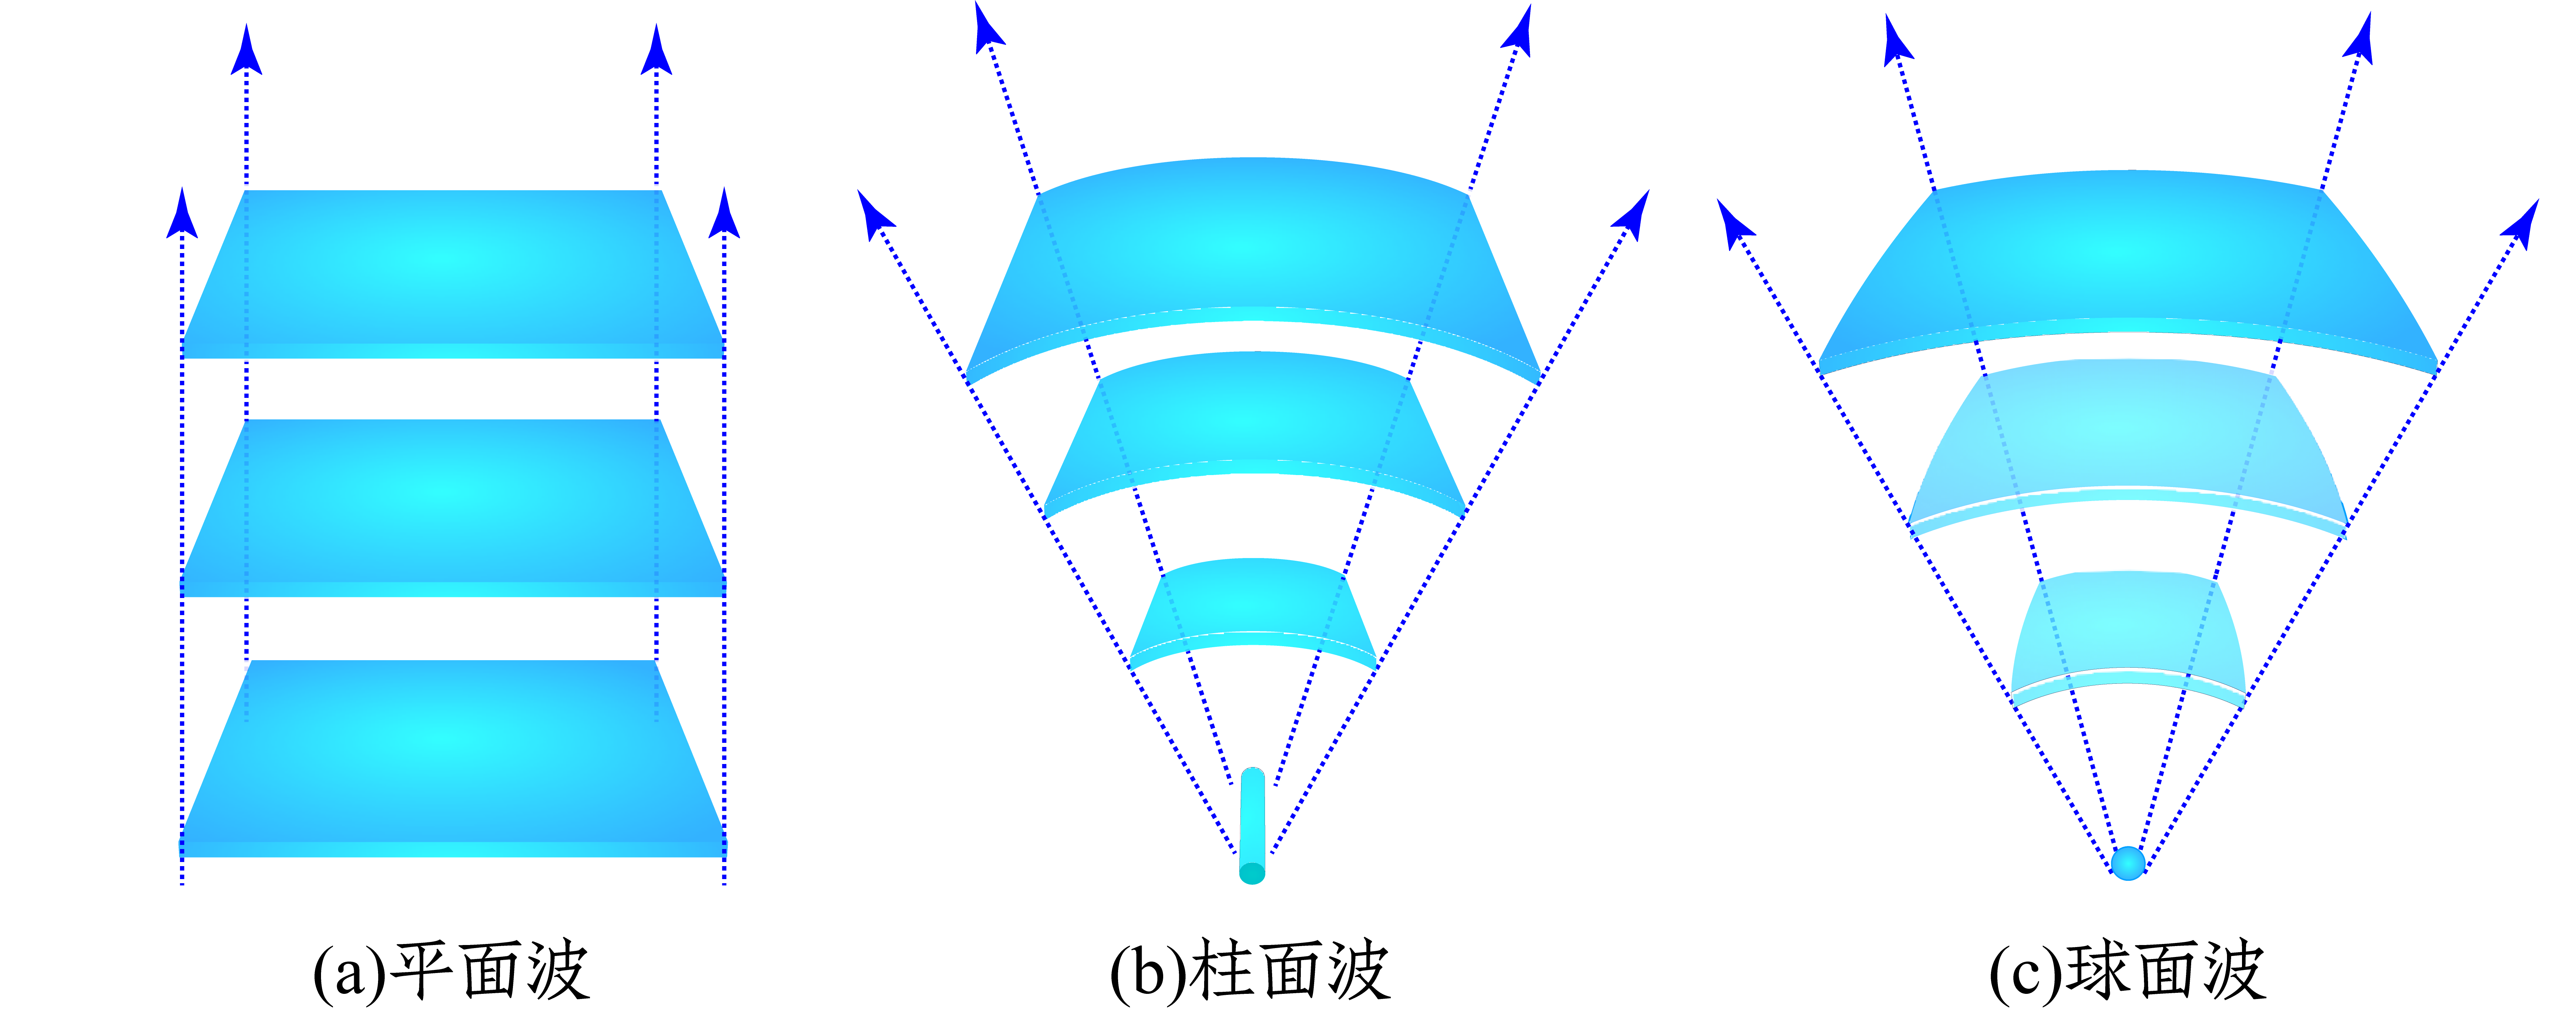
\includegraphics[width=0.8\textwidth]{image/14-1-1.png}
\caption{三种典型的波}
\end{figure}

\begin{enumerate}
	\item $A(\bs{r},\,t)=A\cos(\omega t-\bs{k}\cdot \bs{r}+\phi)$

	要求$\dfrac{\omega}{|\bs{k}|}=c$.\,此为传播方向为$\bs{k}$的平面行波.
	\item $A(\bs{r},\,t)=\dfrac{I}{\sqrt{\rho}}\cos(\omega t-k\rho+\phi)$

	要求$\dfrac{\omega}{|k|}=c$.\,$k>0$时为向外传播的柱面行波,\,$k$小于零则向内传播.
	\item $A(\bs{r},\,t)=\dfrac{I}{r}\cos(\omega t-kr+\phi)$

	要求$\dfrac{\omega}{|k|}=c$.\,$k>0$时为向外传播的球面行波,\,$k$小于零则向内传播.
\end{enumerate}

容易发现,\,以上波全都具有这样的形式:
\[A(\bs{r},\,t)=|A|(\bs{r})\cos(\omega t-\varphi(\bs{r}))\]

也就是说,\,每个点的相位都在以共同的$\omega$做等速率的增加,\,代表一种同步的振动.\,而振动幅度$|A|>0$是要由于波的传播特点和能量流动的连续性而缓慢变化的.\,具体传播方向则看相位的梯度:
\[\bs{k}=+\nabla \varphi\]

在近似的意义下,\,$\dfrac{\omega}{|\bs{k}|}=c$是没有问题的.\,而$c$便是波传播的速度.\,在真空与介质(写作$v$)中出现在光的波动方程中的$\dfrac{1}{c^2}$中的$c$其实是:
\[c=\frac{1}{\sqrt{\varepsilon_0\mu_0}}\quad ,\quad v=\frac{c}{n},\,n=\sqrt{\varepsilon_r\mu_r}\approx \sqrt{\varepsilon_r}\]

约等于符号是因为考虑到了透明光学介质一般磁性质不显著故$\mu_r\approx 1$.

我们不是很推荐用三角函数来计算波动光学.\,要写成复指数的形式,\,而实际三角函数理解为它的有效的实部,\,虚部是为了方便计算而添加的没有物理效应的.\,而且波动光学统一约定,\,利用三角函数的形式,\,为相位增添一个负号,\,使得光在同一刻沿传播方向相位是增加的,\,改为:
\[A(\bs{r},\,t)=|A|(\bs{r})\ue^{\ui(\varphi(\bs{r})-\omega t)}=|A|(\bs{r})\ue^{\ui\varphi(\bs{r})}\ue^{-\ui\omega t}=A(\bs{r})\ue^{-\ui\omega t}\]

在以后情形下我们都将把这种符号约定称为``光学符号约定'',\,而以往的指数上的宗量随时间增加随传播方向减小的符号约定称为``电磁学符号约定''.\,以上讨论就引出了复振幅$A(\bs{r})$的概念.\,而之前找到的各点振幅$|A|$和$\varphi$现在就被整合在了一起,\,作为了复振幅的模与幅角:
\[|A|(\bs{r})=|A(\bs{r})|\quad ,\quad \varphi(\bs{r})=\arg A(\bs{r})\]

回过头来再看,\,我们在解波动方程时,\,实际上从一开始就没有必要认为该标量$A(\bs{r},\,t)$是一个实数,\,在复数域内解,\,也能够直接得到完全与上述等效一样的结果.\,最后我们发现,\,该复数标量场$A(\bs{r},\,t)$如果能够符合波动方程,\,其实部与虚部也是能够分别满足波动方程的:
\[\left(\nabla^2 -\frac{1}{c^2}\frac{\partial^2}{\partial t^2}\right)A(\bs{r},\,t)=0\quad \Rightarrow \begin{cases}\left(\nabla^2 -\dfrac{1}{c^2}\dfrac{\partial^2}{\partial t^2}\right)\mathfrak{Re} A(\bs{r},\,t)=0 \\[8pt] \left(\nabla^2 -\dfrac{1}{c^2}\dfrac{\partial^2}{\partial t^2}\right)\mathfrak{Im}A(\bs{r},\,t)=0\end{cases}\]

如果再要求这样的$A(\bs{r},\,t)$具有形式$A(\bs{r},\,t)=A(\bs{r})\ue^{-\ui\omega t}$,\,数学上也就是对变量$t$分离变量,\,物理就意味着研究单色光的传播,\,那么代入便会发现实际上$A(\bs{r})$需要满足的对空间的方程为\emph{亥姆霍兹方程}(helmholtz equation):
\[(\nabla^2+k^2)A(\bs{r})=0\quad ,\quad k=\frac{\omega}{c}\]

这就是整个波动光学理论的核心方程.\,在继续阐述之前我们先说说$A$指什么.\,其实真空与线性介质(不导电)电磁场几乎每个量(标势,\,矢势,\,电场,\,磁场)都是符合波动方程的:
\[A:\;\{\varphi,\, A_x,\,A_y,\,A_z,\,E_x,\,E_y,\,E_z,\,B_x,\,B_y,\,B_z\}\]
\[\left(\nabla^2 -\frac{1}{c^2}\frac{\partial^2}{\partial t^2}\right)A(\bs{r},\,t)=0\quad,\quad (\nabla^2+k^2)A(\bs{r})=0\]

所以作为复数的标量波理论就构成了光干涉,\,衍射等波动光学课题的数学基础.\,而且我们率先注意到其中的两点:


一是,\,波动方程,\,亥姆霍兹方程是线性方程,\,也就是说,\,如果两个光场都符合方程,\,那么两个场直接逐点做标量加法得到的场也会自动符合方程.\,这也就是之后干涉,\,衍射操作的重要前提.\,如果由于两个原因同时产生了两束光波,\,那么只要写出各自的场,\,加在一起便是整个体系现在的光场.\,这就是双光束干涉时我们将会采取的做法.


二是,\,平面波与球面波的重要性.\,只要是行波,\,在任意一点就可以按照平面波来近似.\,如果取其$\bs{k}$方向为$z$方向,\,那么局部的光场为:
\[A(\bs{r})=A\ue^{\ui kz}\]

\begin{wrapfigure}[10]{o}[0pt]{10cm}
\centering
\vspace{-0.1cm}
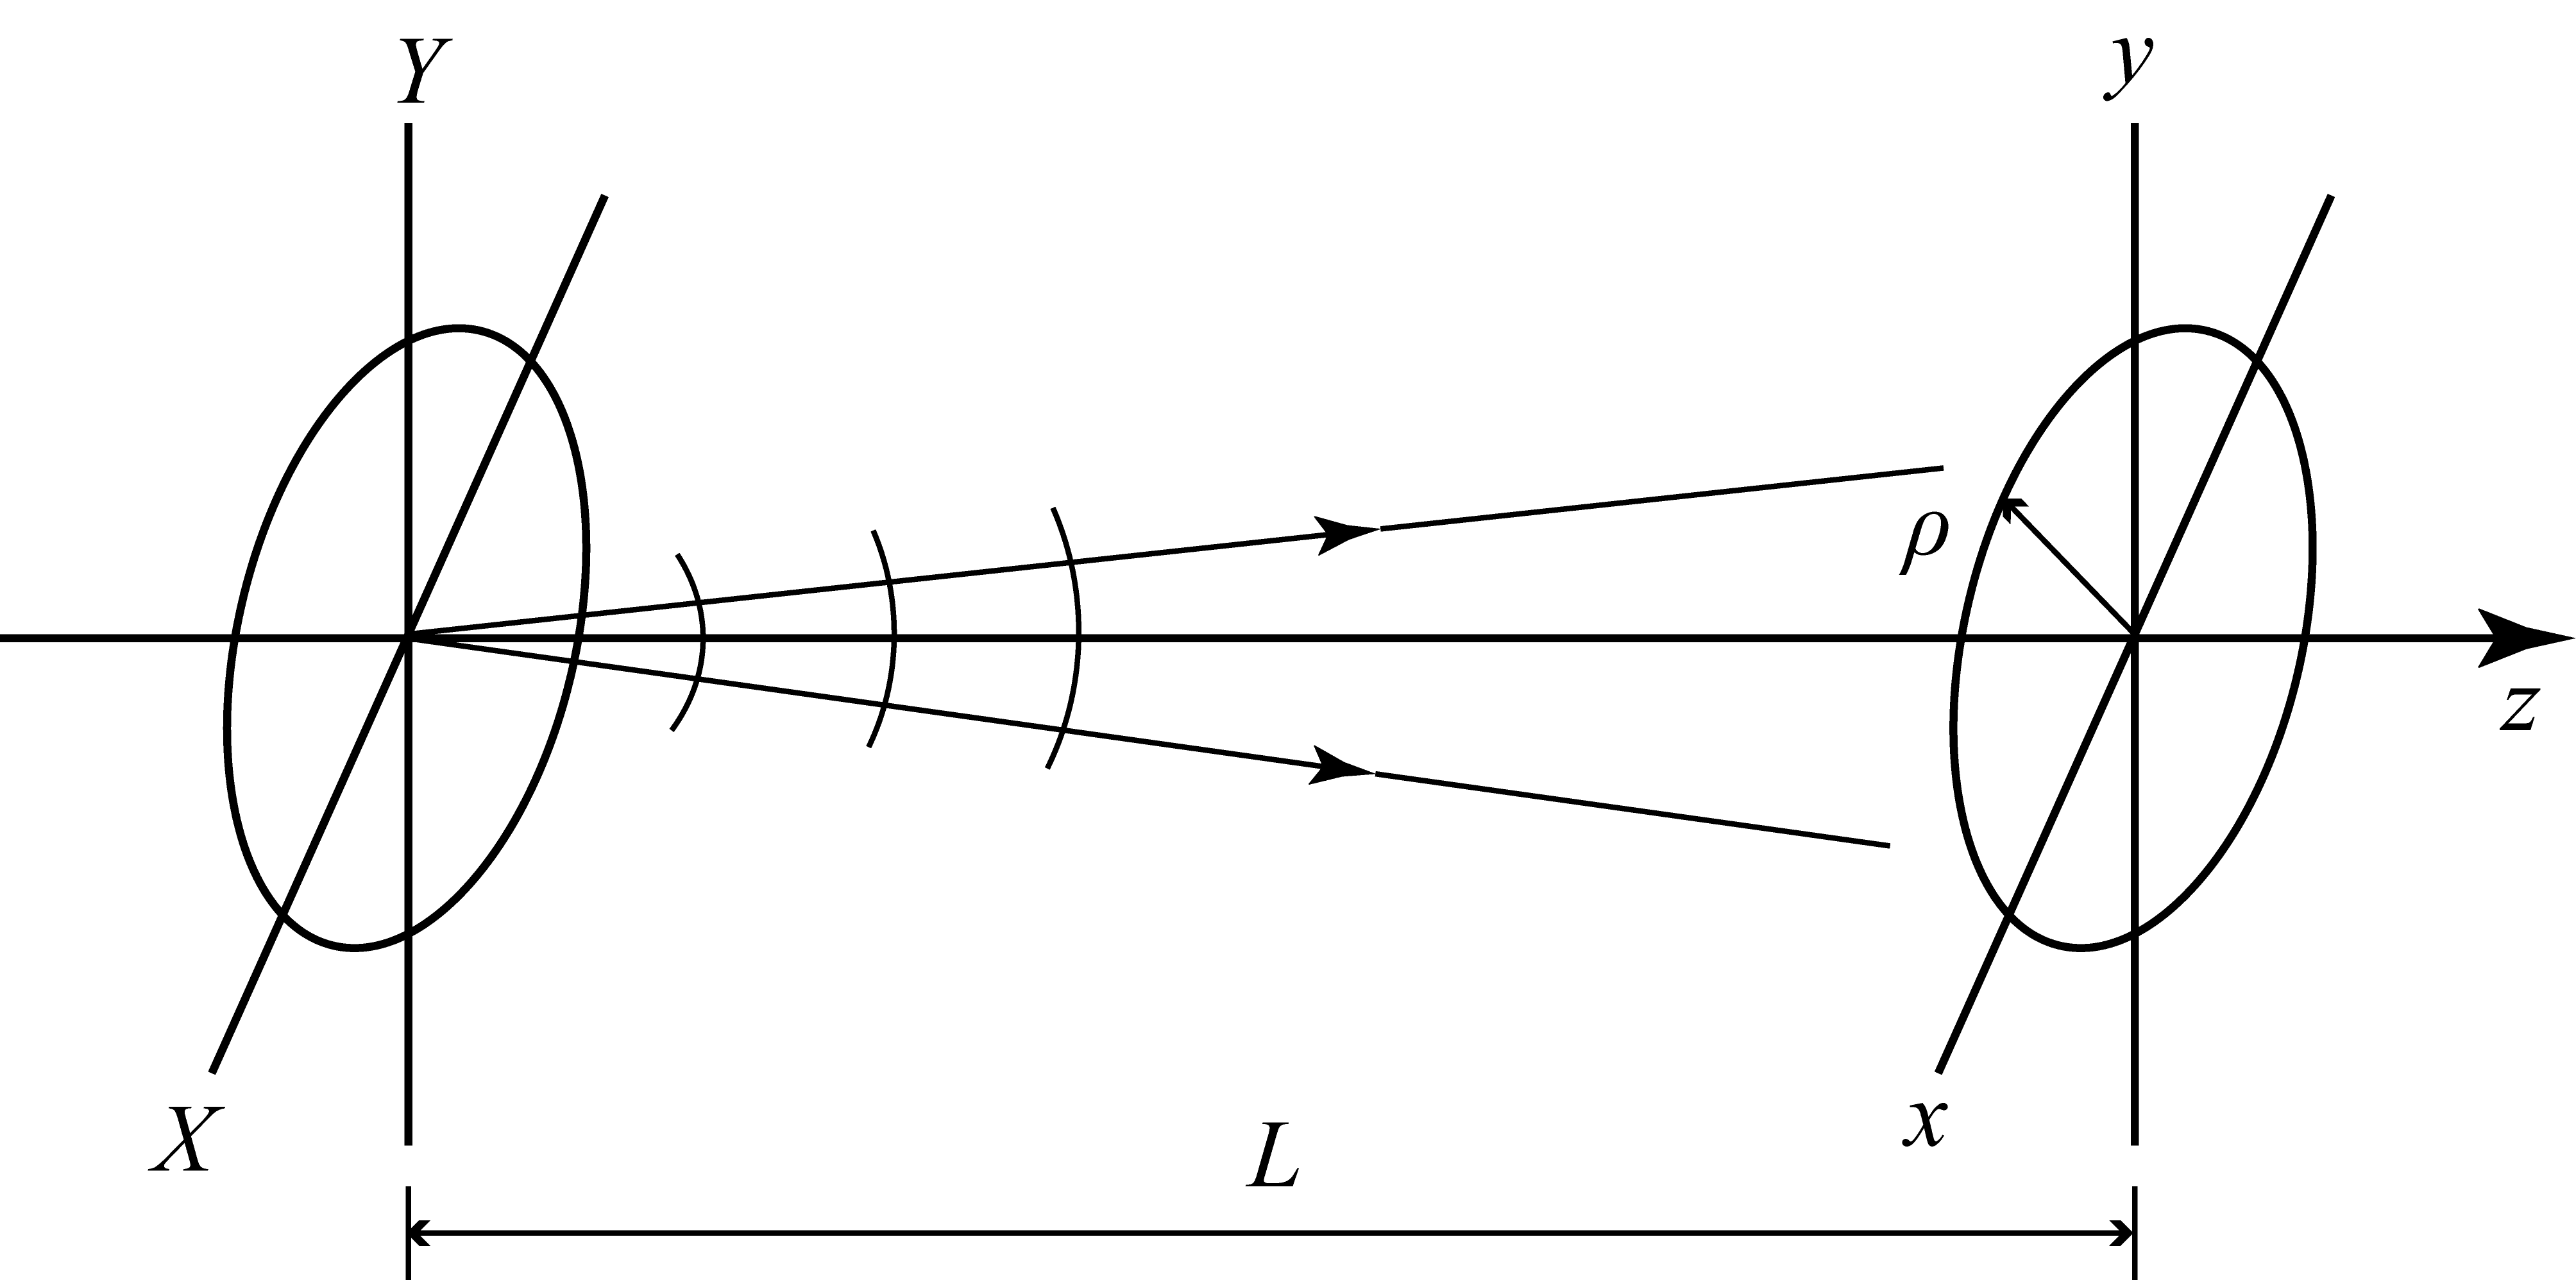
\includegraphics[width=10cm]{image/14-1-2.png}
\caption{球面波向平面波近似}
\end{wrapfigure}
但是旁边的点$(x_1,\,y_1)$的最佳平面波的近似却不一定平行于$z$轴,\,它应该为:
\[A(\bs{r})=A\ue^{\ui [k_z z+k_x (x-x_1)+k_y (y-y_1)]}\]

这下便有第一个近似条件了,\,我们叫做\emph{傍轴条件}(paraxial condition).\,它要求光线传播方向与$z$轴夹一个小角度.\,此时我们习惯把$x$和$y$方向方向余弦$\cos \alpha_x,\,\cos\alpha_y$使用的约$90$度的角度$\alpha_x,\,\alpha_y$的余角记做方向角,\,也就是说:
\[\sin \theta_x\approx \theta_x=\frac{k_x}{k}\quad,\quad \sin \theta_y\approx \theta_y=\frac{k_y}{k}\quad,\quad k_z\approx \sqrt{1-\theta^2_x-\theta^2_y}k\approx k\]

在傍轴近似下,\,以上以方向角$(\theta_x,\,\theta_y)$传播的平面波被方便地写为:
\[A(\bs{r})=A\ue^{\ui k z}\ue^{\ui\phi}\ue^{\ui k (\theta_x x+\theta_y y)}=A'\ue^{\ui k (\theta_x x+\theta_y y)}\]

经常的,\,我们只需要关心在像屏$z=0$上的场,\,参考上图.\,所以上式我们可以把不变的系数都统一写作$A'$.

但是平面波却不总是好的近似,\,我们已经发现了,\,像上图那样,\,如果在物屏$z=-L$上原点$X=0,\,Y=0$处有一点光源发出球面波,\,那么光屏上$(0,\,0)$处和$(x_1,\,y_1)$处的近似公式就采取了不同的形式.\,所以我们会寻求更好的球面波近似.\,但且慢,\,是不是任意情况下光场中的任意一点附近的场都能近似为一个球面波呢?\,答案显然是否定的.\,比如柱面波很显然就不能被近似为球面波,\,因为其\emph{波前}(wavefront),\,即等相位面沿垂直于传播方向的一个方向弯曲而另一个方向却是平直的.\,事实上球面波的光源是点,\,柱面波的光源是线.\,而介于柱面波与球面波中间的某种不对称波前就连光源都没法找到.\,但是球面波的地位仍然是重要的.\,这体现在两点上.\,一是在真实的光路系统中,\,点光源是切实存在且常用的.\,此时物方到像方的点到点的消除了像差的理想成像是我们努力追求的方向.\,故在这样的系统中光波的确一直都适合被近似为球面波,\,而平面波也被当做一种光源在无穷远的特殊状态而处理.\,二是,\,若把波前上各个点当成是新的次波源向前发射出球面波而在前方相干叠加形成新的光场,\,后面在衍射这一章我们数学上可以证明这就是计算光的传播的正确方式.\,其中用到的球面波作为一种本质上重要的物理对象,\,即\emph{传播子}(propagator),\,有着重要的物理地位.

故我们研究从物屏$z=-L$的$(X,\,Y)$处传播到像屏$z=0$处$(x,\,y)$点的球面波的场:
\begin{align*}
A(x,\,y)	&=\frac{I}{\sqrt{L^2+(x-X)^2+(y-Y)^2}}\ue^{\ui k\sqrt{L^2+(x-X)^2+(y-Y)^2}}\\
			&=\frac{I}{L}\ue^{\ui kL}\left[1+\frac{(x-X)^2}{L^2}+\frac{(y-Y)^2}{L^2}\right]^{-\frac{1}{2}}\ue^{\ui kL\left[\left[1+\frac{(x-X)^2}{L^2}+\frac{(y-Y)^2}{L^2}\right]^{\frac{1}{2}}-1\right]}
\end{align*}

由于傍轴条件,\,我们发现方向角$(u_x,\,u_y),\,u_x=\dfrac{x}{L},\,u_y=\dfrac{y}{L}$和方向角$(U_x,\,U_y),\,U_x=\dfrac{X}{L},\,U_y=\dfrac{Y}{L}$都是小量,\,而传播到光屏上该点的光的方向角($\bs{k}$方向)为$(u_x-U_x,\,u_y-U_y)$.\,仅考虑领头项,\,把不随$x,\,y$变化的系数记为常数,\,我们发现:
\[A(x,\,y)=A\ue^{\frac{\ui}{2}kL[(u_x-U_x)^2+(u_y-U_y)^2]}=A'\ue^{\ui k\frac{x^2+y^2}{2L}}\ue^{-\ui k\frac{Xx+Yy}{L}}\]

也就是说光屏上的波由两个相因子决定.\,第一个是平方相关于$x,\,y$的$\varphi_1=k\dfrac{x^2+y^2}{2L}=\pi \dfrac{x^2+y^2}{\lambda L}$,\,第二个恰好是平面波的相因子$\varphi_2=-k\dfrac{Xx+Yy}{L}=-k(U_x x+U_y y)=k(\theta_x x+\theta_y y)$.\,就是说当点光源相对$(x,\,y)=(0,\,0)$从$X<0,\,Y<0$的方向照过来能够在原点附近获得方向角为正的平面波场.

那么球面波能够被近似为球面波的条件也就不言自明了,\,它要求第一个相因子的相位很小不干扰第二个相因子,\,也就是$\varphi_1\ll \pi$,\,也就是\emph{远场条件}(farfield condition):
\[\rho^2\ll \lambda L\quad \Leftrightarrow \quad L\gg \frac{\rho^2}{\lambda}\]

其实换一个角度理解这个条件,\,如果远场条件被满足,\,但是在这样的$\rho$内第二个相因子变化也非常小时,\,整个$A$几乎就是常数,\,这时候也形成不了有价值的光场,\,所以我们如果要求$\varphi_2\gg \varphi_1$,\,还能发现第三个条件$X,\,Y\gg x,\,y$.\,对于这个条件我们做这样的理解,\,相位的绝对大小是没有观测效果的.\,我们需要的其实是光束干涉时相位的差值.\,故这其实是要求物屏的花样尺寸要远大于像屏上干涉花样的观测范围.

在远场条件不被满足的情况下,\,考虑第一个相因子对第二个相因子的影响,\,会造成干涉图样的扭曲与形变,\,几何光学上会造成最基础的像差:\,相散和散焦.

在介绍下两节具体的干涉之前,\,对干涉的原理做一个简要的介绍是有必要的.\,根据之前的介绍,\,空间中如果同时存在两个光场:
\[A_1(\bs{r})=|A_1|(\bs{r})\ue^{\ui\varphi_1(\bs{r})}\quad ;\quad A_2(\bs{r})=|A_2|(\bs{r})\ue^{\ui\varphi_2(\bs{r})}\]

我们可以找到其单独存在时的光强,\,一般来说,\,光强为位置的缓变函数:
\[I_1(\bs{r})=|A_1|^2=A_1^\ast A_1 \quad ;\quad I_2(\bs{r})=|A_2|^2=A_2^\ast A_2\]

然而光场的叠加是有两种典型的方式的.\,最常见的其实是\emph{非相干叠加}(incoherent superposition).\,此时出于下面要介绍的原因,\,光强是可以逐点直接相加的:
\[I(\bs{r})=I_1(\bs{r})+I_2(\bs{r})\]

将自然界或人造的两束来源不同的光照在一次是无法观察到干涉花样的.\,光的干涉条件比机械波干涉条件来的苛刻的多.\,在某些细心制备的实验室条件下才能观察到干涉花样,\,此时光场是\emph{相干叠加}(coherent superposition).\,在光学之中相干度是十分值得关注的.\,我们将在之后的一节中集中讨论.\,读者可能自然地认为相干叠加时为复振幅相加:
\[A(\bs{r})=A_1(\bs{r})+A_2(\bs{r})\]

但是其实无论非相干叠加还是相干叠加上式都适用,\,那么是什么造成了两者的区别呢?\,我们把上式模方求光强:
\begin{align*}
I(\bs{r}) &=A^\ast A \\
		  &=(A_1^\ast +A_2^\ast)(A_1+A_2) \\
		  &=A_1^\ast A_1+A_2^\ast A_2+ A_1^\ast A_2+A_2^\ast A_1 \\
		  &=I_1+I_2+ |A_1||A_2|\ue^{\ui (\varphi_2-\varphi_1)}+|A_1||A_2|\ue^{\ui (\varphi_1-\varphi_2)} \\
		  &=I_1+I_2+ 2\sqrt{I_1I_2}\cos (\varphi_2-\varphi_1)
\end{align*}

上式中出现的交叉项$2\sqrt{I_1I_2}\cos (\varphi_2-\varphi_1)$就叫\emph{干涉项}(interference term).\,它是关于位置的快变函数.\,乍一看这也未免太快了,\,因为只要当空间位置改变一个波长,\,相位$\varphi$就会有$\pi$的量级的改变,\,这样干涉项在这个过程中就会有正负号的改变.\,从而产生干涉花样.\,在实际的干涉实验中,\,合理的仪器设置可以使得这个空间特征长度被放大到人眼或助视仪器可以直接观测的程度.\,从而这就是干涉实验的基础.

那么为什么对于非相干叠加情形我们直接去掉了干涉项.\,那是因为在之前我们做把光场向标量复振幅简化的过程中去掉了公共的单色光时间演化项$\ue ^{\ui \omega t}$.\,这并不是永远合理的做法.\,真实光场由于后面要介绍的各种原因,\,可以认为相位随时间的演化并不是完全线性增加的而是有随时间偏离期望值的方差越来越大的涨落.\,从而两束并没有关联的自然光之间不同时刻同一点$\bs{r}$的相位差$\delta=\varphi_2(\bs{r})-\varphi_1(\bs{r})$是一个在随机涨落的数,\,只要涨落够大,\,$\cos (\varphi_2-\varphi_1)$项的随时间平均就会总是趋近于零.\,从而干涉现象也就消失了.

在以下的两小节中,\,我们先不用关心相干性的问题,\,认为不同光场的叠加总是有``完美的相干性'':\,完全稳定的相位差.\,我们会在不同干涉装置的介绍中去强调为什么总是能保证``完美的相干性''的成立.




\section{分波面干涉}

以下几种干涉装置一般统一归为\emph{分波面干涉}(interference by dividing wave-front).\,因为它们实现的核心思想都是让本来沿各个方向独立传播的波前的部分改变传播方式而在空间中产生交叠.

%\subsection{杨氏双缝干涉仪}

历史上第一个挑战牛顿光的粒子说权威,\,构想出更合理的光的波动说的假设并通过实验证明自己的想法的是谁?\,那必然要归功于\emph{托马斯·杨}(Thomas Young)\footnote{杨氏为英国博物学家,\,也经常作为物理学家而介绍.\,除了双缝实验,\,也因为杨氏模量,\,杨-亥姆霍兹三色视觉论,\,杨-拉普拉斯和杨-杜普蕾附加压强与接触角公式而闻名.\,他还是杰出的语言学家,\,比较了400钟语言的词汇与语法.\,并解密了一部分古埃及象形文字.\,在音乐,\,医学和神学等上也有贡献.}.\,

\section{分振幅干涉}

\section{偏振干涉}

\section{相干性}

\section{多光束干涉}


%!TEX root = ../physical-olympics-2.tex
\chapter{光的衍射}


\section{光栅与波带片}
\begin{itemize}
\item 光栅衍射:\,光栅常数,\,即空间周期为$d$,\,缝宽为$a$,\,总共刻$N$道.\,那么:
\[I=I_0\cdot f_1(\theta)\cdot \left(\frac{\sin N\beta}{\sin \beta}\right)^2\quad, \quad \beta=\frac{\pi d}{\lambda}\sin \theta\]

其中$f_1(\theta)$为之后可以算出来的与单缝衍射有关的慢变(需要$a<<d$)的单元因子:
\[f_1(\theta)=\left(\frac{\sin \alpha}{ \alpha}\right)^2\quad, \quad \alpha=\frac{\pi a}{\lambda}\sin \theta\]

体现光栅的结构的是后面的结构因子:
\[f_2(\theta)=\left(\frac{\sin N\beta}{\sin \beta}\right)^2\quad, \quad \beta=\frac{\pi d}{\lambda}\sin \theta\]

从中可以得到三个信息:\,主极大方向$d\sin\theta_j=j\lambda$,\,主极大强度$I=N^2 I_0$,\,主极大宽度$\delta\theta\sim j\lambda/Nd$

\item 圆孔菲涅尔衍射:\,波带法与半波带法.\,核心在于以下等式:
\[\frac{\ud S}{r}={\rm const.}\cdot \ud r\]

\begin{figure}[H]
\centering
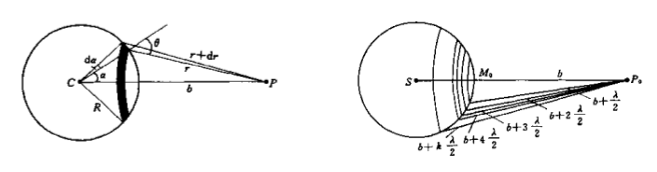
\includegraphics[width=0.8\textwidth]{image/14-2-2.png}
\caption{波带法与半波带法}
\end{figure}

这说明不同位置的波前上的带状面元,\,根据其对要计算的点所造成的光程差,\,相等的光程差造成完全相等的振幅,\,尽管面元的面积不相等.\,只需要把这些振幅相等,\,相位不等的光矢量进行合成.

合成方法一般有两种,\,对于半波带问题把面元分解为半波带显得方便.\,而复杂问题需要按照微元分解,\,下一节将介绍面元对要计算的点的光矢量贡献还有一个起到调制作用的角度因子,\,故合成图像一般为:
\begin{figure}[H]
\centering
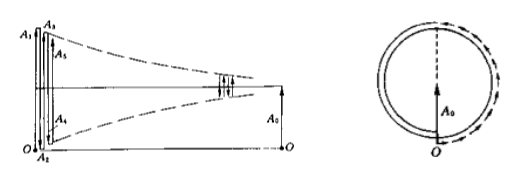
\includegraphics[width=0.8\textwidth]{image/14-2-3.png}
\caption{分组合成与积分合成}
\end{figure}

\item 波带片:\,预想将一点光源和一要计算光强的点中间合适距离处的波前按照半波带分解,\,再制造一光学器件,\,或者遮住奇数半波带而开放偶数半波带,\,或者遮住偶数半波带而开放奇数半波带.\,就构成了波带片.\,如果在一张圆形的片上入射平行光,\,而选取距离为$f$的点计算光程,\,那么各个半径为:
\[\rho_j=\sqrt{j\lambda f}\]

这样的波带片可以当做一个焦距为$f$的透镜使用.\,但是成像并不唯一,\,容易证明它具有一组虚焦点和实焦点.


\end{itemize}

%\section{布拉格衍射}

\section{衍射积分公式}

\begin{itemize}
\item 基尔霍夫衍射积分公式:
\[A(\bs{r})=\frac{1}{i\lambda}\int \bs{A}(\bs{r}')\cdot F\cdot \frac{e^{\ui k|\bs{r}-\bs{r}'|}\ud S}{|\bs{r}-\bs{r}'|}\]

$F$为角度因子,\,若入射波波矢$\bs{k}'$方向为$\bs{e}'$,\,子波波矢$\bs{k}$方向为$\bs{e}$,\,面元$\ud S$方向为$\bs{n}$,\,则有:
\[F=\frac{\bs{n}\cdot \bs{e}+\bs{n}\cdot \bs{e}'}{2}=\frac{\cos\theta+\cos \theta'}{2}\]

\item 夫琅和费衍射公式:\,如果在衍射屏后放置焦距为$f$的透镜并在后焦面上观察,\,并且忽略角度因子.\,把入射场在衍射屏作用后的波前写作$A(x_0,\,y_0)$.\,那么这个情况具有更简单的公式:
\[A(\theta_x,\,\theta_y)=\frac{1}{\ui\lambda f}\iint A(x_0,\,y_0)e^{-i(k_x x_0+k_y y_0)}\ud x_0\ud y_0\]

\item 矩孔衍射:
\[I=I_0\cdot \left(\frac{ab}{\lambda f}\right)^2\cdot \left(\frac{\sin\alpha}{\alpha}\right)^2\cdot \left(\frac{\sin\beta}{\beta}\right)^2\quad ,\quad \alpha =\frac{\pi a}{\lambda}\sin\theta_x\,,\,\beta =\frac{\pi b}{\lambda}\sin\theta_y\]

\item 圆孔衍射:\,直径$d$,\,艾里斑半角$\theta$:
\[\theta\approx \frac{1.22\lambda 	}{d}\]
\end{itemize}

%\section{波前分析法}

%!TEX root = ../physical-olympics-2.tex
\chapter{物理光学}


\section{经典色散理论}

蓝天,\,白云,\,红太阳.\,在简单的自然现象中蕴含着光在传播过程中的另外一种典型的现象:\,\emph{散射}(scattering).\,而散射却又是一个多么复杂的现象!\,要完全理解散射,\,我们得研究光的吸收与发射,\,因为光与物质中分子的相互作用其实本质上可以看成吸收与发射,\,这是\emph{分子光学}(molecular optics)的研究范畴.\,其次,\,光在介质中的衰减(吸收),\,不同颜色的光折射率的不同(色散)其实都导致了一类散射现象(瑞利散射).\,但是还有不同的散射现象则表现出不用的特性,\,需要从更宏观或更微观的角度去建立新的理论来解释他们.

不同于以往在透明介质中的平面波传播,\,新的现象需要新的平面波模型.

\subsection{复波矢与复折射率}

我们在波动方程的解中引入复数是为了更好地描述振动形式的解.\,但这却忽视了另一种解的存在性.\,就是如果波矢$\bs{k}$本身亦为复数,\,由于同时又是一个矢量,\,可以表示为$\bs{k}=\bs{\alpha}+\ui\bs{\beta}$.\,代入场的空间部分:
\[A(\bs{r})=A_0\ue^{\ui \bs{k}\cdot \bs{r}}=A_0\ue^{- \bs{\beta}\cdot \bs{r}}\ue^{\ui \bs{\alpha}\cdot \bs{r}}\]

这就代表了一个沿$\bs{\alpha}$方向传播,\,沿$\bs{\beta}$方向衰减的平面波.\,而$\bs{\alpha}$为波矢的实部,\,$\bs{\beta}$为波矢的虚部:
\[\bs{\alpha} =\mathfrak{Re} (\bs{k})\quad;\quad \bs{\beta}=\mathfrak{Im} (\bs{k})\]

这种波可不可以在真空中传播?\,出人意料的是这居然是可能的.\,因为如果代入真空中的亥姆霍兹方程:
\[\nabla ^2 A+\frac{\omega^2}{c^2}A=0\]

便会发现这只需要要求:
\[\bs{k}^2=(\bs{\alpha}+\ui \bs{\beta})\cdot(\bs{\alpha}+\ui \bs{\beta})=\frac{\omega^2}{c^2} \quad \Rightarrow \quad \alpha^2-\beta^2=\frac{\omega^2}{c^2},\,\bs{\alpha}\cdot\bs{\beta}=0\]

\begin{wrapfigure}[12]{o}[0pt]{7cm}
\centering
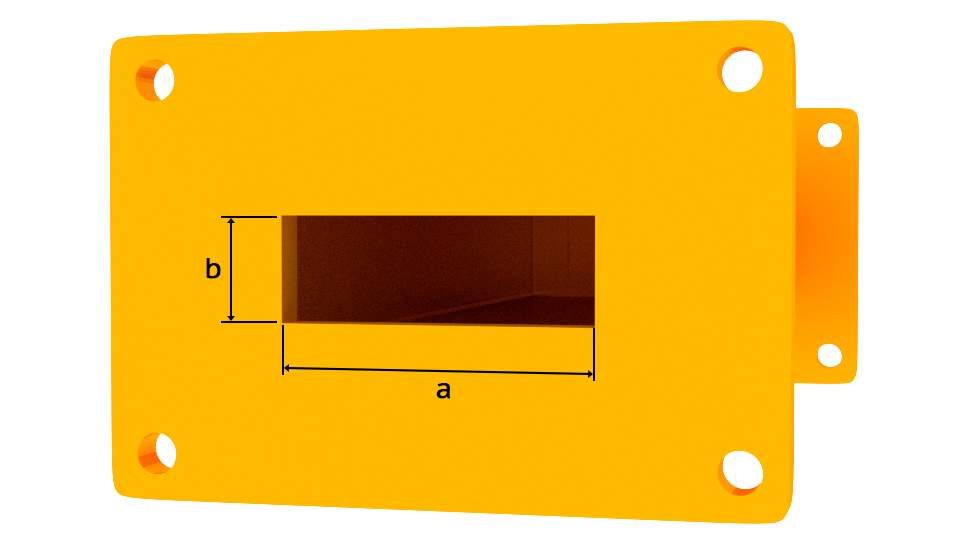
\includegraphics[width=7cm]{image/16-1-1.jpg}
\caption{矩形波导}
\end{wrapfigure}
这样的波我们并不陌生,\,早在几何光学我们介绍光的全反射时便研究过另一侧界面中的隐失波场便是以上形式.\,更典型地,\,在$a\times b$的矩形波导中传播的波满足:
\[(\frac{2\pi}{\lambda_x})^2+(\frac{2\pi}{\lambda_y})^2+(\frac{2\pi}{\lambda_z})^2=\frac{\omega^2}{c^2} \]
\[\lambda_x=\frac{2b}{m},\, \lambda_y=\frac{2a}{n},\,m,\,n=1,\,2\cdots\]

此时在$x,\,y$方向的振动是驻波,\,$z$方向传播的波则是行波.\,$x,\,y$方向要形成驻波是因为在边界的导体上要符合相同的边界条件,\,所以或都是波腹,\,或都是波节.\,亦可以用同一个平面波在侧面上的多次反射的叠加来理解这种兼具驻波和行波特质的场.\,我们发现模式为$(m,\,n)$的波,\,会有一个截止角频率$\omega_c$,\,如果角频率低于此值使得波无法向前传播:
\[\omega_c=c\sqrt{\left(\frac{m\pi}{a}\right)^2+\left(\frac{n\pi}{b}\right)^2}\]

那如果在波导的起点的天线给出信号角频率$\omega<\omega_c$会发生什么情况?\,此时就是$z$方向波矢$k_z$变为虚数,\,意味着波沿$z$方向不是传播而是衰减:
\[\bs{k}=\bs{\alpha}+\ui\bs{\beta}\]
\[\bs{\alpha}=\left( \frac{m\pi}{a},\, \frac{n\pi}{b},\, 0\right)\quad,\quad\bs{\beta}=\left(0 ,\,0 ,\, \sqrt{\left(\frac{m\pi}{a}\right)^2+\left(\frac{n\pi}{b}\right)^2-\frac{\omega^2}{c^2}}\right)\]

在真空中尚可以产生衰减的波\footnote{事实上,\,只需要亚波长的结构便可造成衰减.},\,更何况在各种介质中.\,事实上,\,描述光在介质中随着传播的距离而衰减的现象早有一经验公式,\,即\emph{比尔-朗博-布葛律}(Beer-Lambert-Bouguer law):
\[\frac{I(l)}{I(0)}=\ue^{-\left(\sum_{i} n_i\sigma_i\right) l}\]

其中$I(0)$为在传播$l$前的光强,\,$I(l)$为在传播$l$后的光强.\,$n_i$是构成介质的第$i$种分子的数密度,\,$\sigma_i$为描述其吸收本领的\emph{衰减截面}(attenuation cross section).\,例如对大气来说主要的衰减因素就来自气溶胶,\,干净的海水则能提供200m左右的透光带,\,如果有的话,\,浮游植物含有的光合色素是造成衰减的主要原因.\,而对于强衰减性质的介质,\,我们可以唯象地认为波在介质中的传播为:
\[|A(l)|=|A(0)|\ue^{-\beta l}\quad \Rightarrow\quad I(l)=I(0)\ue^{-2\beta l}\]

这样的选择是有道理的.\,下以导电导致的损耗为例:\,在不漏电介质中,\,麦克斯韦关系本应为:
\[\left\{ \begin{array}{l} 
\nabla\cdot \bs{E}=0 \\[3pt] 
\nabla\times \bs{E}+\dfrac{\partial \bs{H}}{\partial t}=\bs{0} \\[3pt]
\nabla\cdot \bs{H}=0 \\[3pt]
\nabla\times \bs{H}-\varepsilon\mu\dfrac{\partial \bs{E}}{\partial t}=\bs{0} \end{array}\right.\]

这样便有:
\[v=\frac{c}{n}=\frac{1}{\sqrt{\varepsilon \mu}}\quad ,\quad k=\frac{\omega}{v}=\omega\sqrt{\varepsilon \mu}\]

但是,\,如果介质漏电,\,且符合$\bs{J}=\sigma \bs{E}$,\,那么以上方程就改写为:
\[\left\{ \begin{array}{l} 
\nabla\cdot \bs{E}=0 \\[3pt] 
\nabla\times \bs{E}+\dfrac{\partial \bs{H}}{\partial t}=\bs{0} \\[3pt]
\nabla\cdot \bs{H}=0 \\[3pt]
\nabla\times \bs{H}-\varepsilon\mu\dfrac{\partial \bs{E}}{\partial t}=\mu_0 \sigma \bs{E} \end{array}\right.\]

对最后一个式子所引发的不同在光学情况下是很好处理的.\,因为单色光总是具有固定的频率$\omega$,\,那么其实以上式子无非是把$\dfrac{\partial}{\partial t}$变成$-\ui \omega$.\,在磁导率被认为几乎等于真空磁导率的情形下,\,这相当于说:
\[\left\{ \begin{array}{l} 
\nabla\cdot \bs{E}=0 \\ 
\nabla\times \bs{E}-\ui \omega \bs{H}=\bs{0} \\
\nabla\cdot \bs{H}=0 \\
\nabla\times \bs{H}+\ui \omega \varepsilon\mu\bs{E}=\bs{0} \end{array}\right. \qquad \xrightarrow{\varepsilon\rightarrow \varepsilon+\ui \frac{\sigma}{\omega}} \qquad
\left\{ \begin{array}{l} 
\nabla\cdot \bs{E}=0 \\
\nabla\times \bs{E}-\ui \omega \bs{H}=\bs{0}  \\
\nabla\cdot \bs{H}=0 \\
\nabla\times \bs{H}+\ui \omega \varepsilon\mu\bs{E}-\ui\sigma \mu \bs{E}=\bs{0} \end{array}\right.
\]

所以对于漏电介质\footnote{即使不漏电,\,也会由于有损耗而等效于有复电容率.},\,通常会有\emph{复电容率}(complex permittivity)的说法\footnote{对于普通的导体,\,也一样可以讨论复电容率,\,或者更常见地,\,\emph{复电导率}(complex conductivity).\,它不仅包含由于原子实部分极化导致的电容性,\,还要包含由于电子运动惯性导致的电感性.},\,它就是以上把电容率和电导率合并以后的新的复常数,\,用它第四个方程就与真空中的方程没有任何区别了,\,除了系数是一个复数:
\[\varepsilon^\prime =\varepsilon+\ui\frac{\sigma}{\omega}:\quad \nabla\times \bs{H}+\ui \omega \varepsilon^\prime\mu\bs{E}=\bs{0}\]

这样一个方程的解是可以完全照搬之前的解的,\,因为数学上可以证明复数解具有可\emph{解析延拓}(analytic continuation)的特性.\,从而容易发现,\,复波矢就变为:
\[\bs{k}^2=\omega^2\varepsilon^\prime \mu\]

这样就得到:
\[\alpha^2-\beta^2=\omega^2\varepsilon \mu\quad ,\quad 2\bs{\alpha}\cdot\bs{\beta}=2\alpha\beta\cos\theta=\omega\sigma\mu>0\]

此时传播波矢$\bs{\alpha}$与衰减波矢$\bs{\beta}$就不一定要垂直了,\,它们必须夹锐角,\,也就是说,\,如果电磁波在漏电介质或者导体中传播,\,沿传播方向必须要衰减.\,我们最后引入光学中使用最多的\emph{复折射率}(complex refraction index),\,按照原来的看法它意味着$k^2=n^2k_0^2=n^2\dfrac{\omega^2}{c^2}=\dfrac{\omega^2}{v^2}$.\,现在要更小心些,\,因为$\bs{k}=\bs{\alpha}+\ui \bs{\beta}$已经包含两个不贡献的波矢部分.\,故我们先对以下表达式开方:
\[\alpha^2-\beta^2+2\ui \alpha\beta\cos\theta=\omega^2\varepsilon^\prime \mu\]
\[\Rightarrow \quad \sqrt{\alpha^2-\beta^2+2\ui \alpha\beta\cos\theta}=n\frac{\omega}{c}=(n_1+\ui n_2)\frac{\omega}{c}\]

通过以上两式对比,\,我们能得到两个方面.\,第一是复折射率实部$n_1$与虚部$n_2$分别是这样依赖于相对介电常数$\varepsilon_r=\varepsilon/\varepsilon_0$和电导率$\sigma$的:
\[n_1=\sqrt{\varepsilon_r}\cdot \sqrt{\frac{1}{2}\left(1+\frac{\sigma^2}{\omega^2\varepsilon^2}+\sqrt{1+\frac{\sigma^2}{\omega^2\varepsilon^2}}\right)}\]
\[n_2=\frac{\sigma}{\sqrt{\varepsilon_r}\omega\varepsilon_0}\cdot\sqrt{\frac{1}{2}\left(1+\frac{\sigma^2}{\omega^2\varepsilon^2}+\sqrt{1+\frac{\sigma^2}{\omega^2\varepsilon^2}}\right)^{-1}}\]

第二组关系式如果已知了介质的两个折射率,\,那么在介质中传播的波的两个波矢$\alpha$和$\beta$需要满足的关系为:
\[\alpha^2-\beta^2=(n_1^2-n_2^2)\frac{\omega^2}{c^2}\]
\[\alpha\beta\cos\theta=n_1n_2\frac{\omega^2}{c^2}\]

只有当$\theta=0$才恰有:
\[\alpha=n_1\frac{\omega}{c}\quad,\quad\beta=n_2\frac{\omega}{c}\]


\subsection{经典电子论的解释}

下面我们来介绍历史上发挥了重要作用的经典电子论.\,它虽然不够精确但物理图像十分重要.

\begin{wrapfigure}[17]{o}[0pt]{6cm}
\centering
\vspace{-3pt}
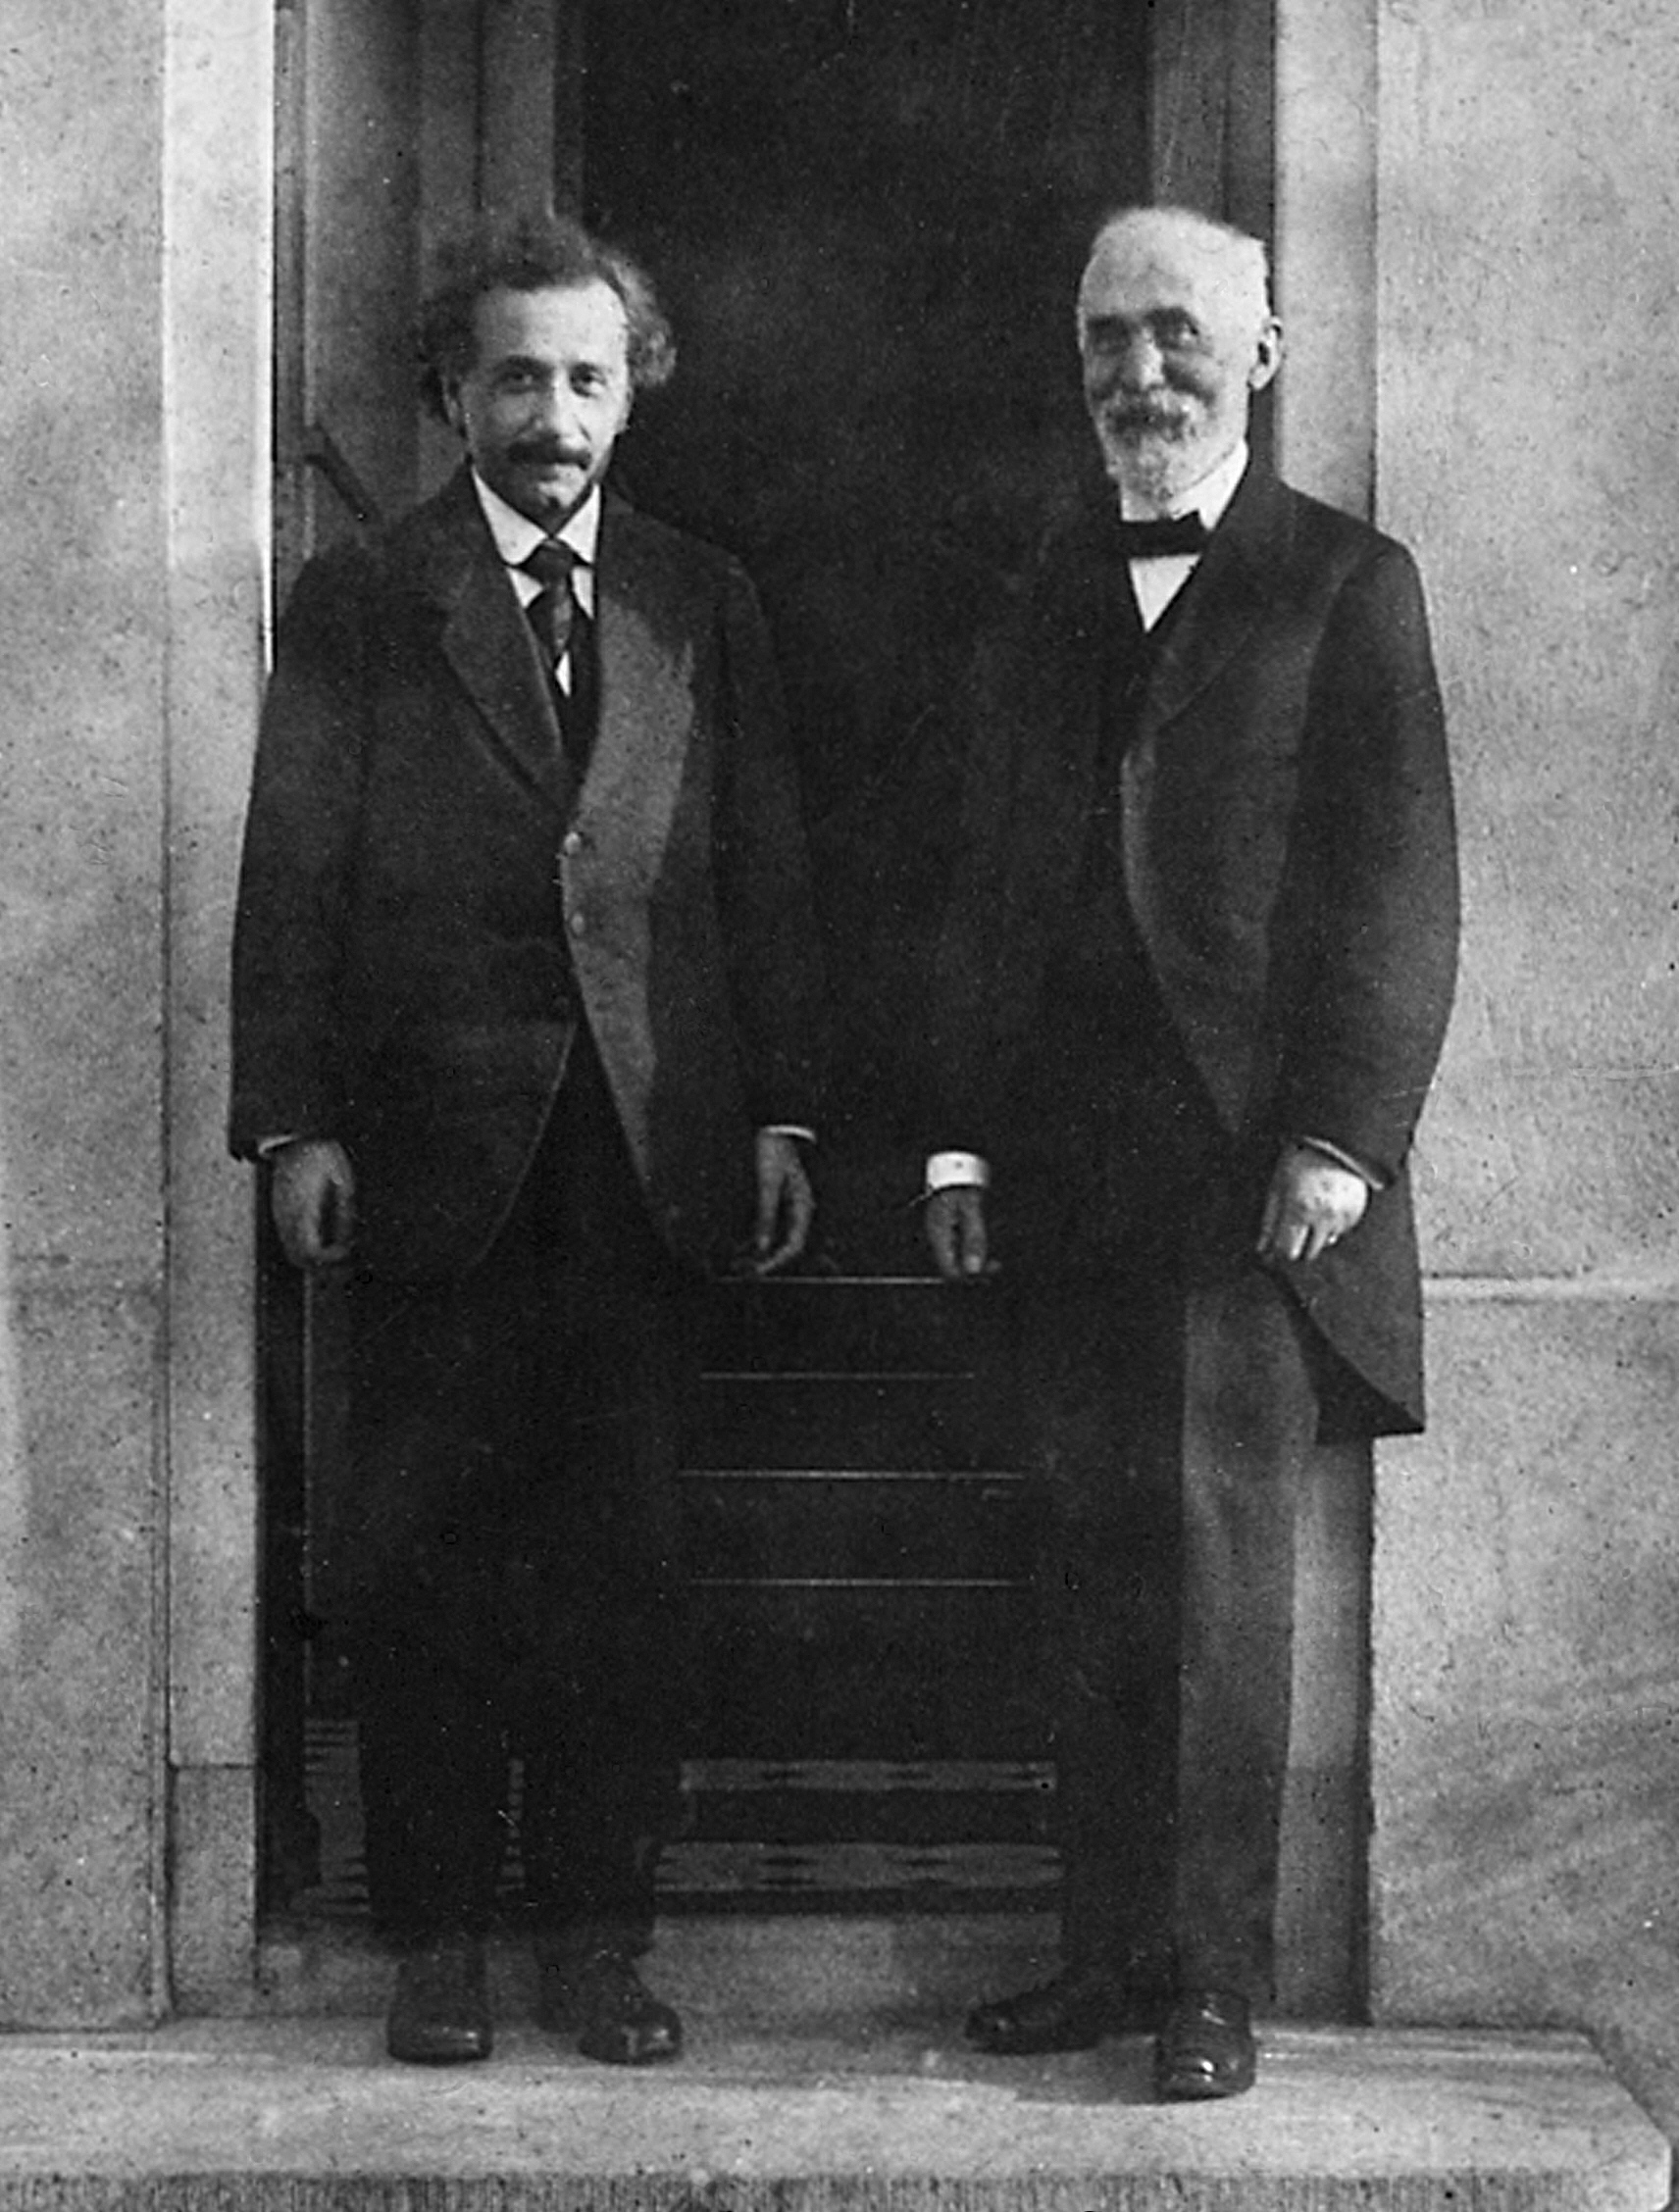
\includegraphics[width=6cm]{image/18-1-2.jpg}
\caption{\rm Einstein与Lorentz}
\end{wrapfigure}

历史上虽然电子作为粒子的发现是1897年\emph{汤姆孙}({\rm J. J. Thomson})的工作.\,但是早在半个世纪前人们就开始逐渐相信物质由两种带电粒子构成并在导电时可以移动的模型了.\,人们用这样的模型去想象输运现象,\,电磁感应,\,热电耦合等现象并取得了丰硕的成果,\,经典电磁学早在1860年代便在\emph{麦克斯韦}({\rm J. C. Maxwell})的工作下达到顶点进入尾声.\,剩下来的几十年时间历史让位给了\emph{洛伦兹}({\rm H. A. Lorentz}),\,洛伦兹对电磁学的贡献是深远的.\,他承前人之大成,\,讨论电磁场与电磁介质的相互作用,\,讨论电磁学原理与古老的伽利略式相对性原理的结合;\,又开近代物理之先河,\,电子论自然地导向了量子理论,\,而电磁学又自然地促成了狭义相对论的诞生.\,事实上,\,早年间狭义相对论在学界被介绍时便是以洛伦兹和爱因斯坦这一对忘年交命名的洛伦兹-爱因斯坦理论.

电子,\,这样一个基本粒子可以说是妇孺皆知的概念,\,它带一个单位的负电荷,\,其基本参数为:
\[e=1.602176634\times 10^{-19}{\rm C}\qquad m_e=9.10938356\times 10^{-34}{\rm kg}\]

然而出于各种原因,\,在经典电子论中的电子却又是一个陌生的概念.\,根据洛伦兹的经典电子论精神,\,重的原子实被认为静止,\,轻的束缚电子被认为在外场中可以运动,\,且主要受电场的影响\footnote{根据洛伦兹力公式$\bs{F}=q(\bs{E}+\bs{v}\times\bs{B})$,\,而电磁场中$E=cB$,\,故$v\ll c$时磁场力可以忽略.}.\,电子在外电场中相对原子实的位移造成了电偶极矩.\,出于好的近似,\,将电子视作被绑在连接中心的弹簧的另一端的质点.\,质量为$m$不再被认为与基本粒子的质量一致,\,事实上这个质量的本质实际上是虚无的,\,因为当考虑到原子与电磁场相互作用的严格理论时图像将完全是量子的而超出了此处可以讨论的范围,\,这样的一个为了解释现象去构造的模型就叫\emph{唯象模型}(phenomenological model).\,但是其电荷量还是$-e$,\,弹簧劲度系数为$k$.\,这样子我们就可以写出电子在外电场中的动力学方程:
\[m\bs{\ddot{r}}+k\bs{r}=-e\bs{E}\]

但是我们还忽略了一点,\,加速运动的电荷会产生辐射,\,也会因为辐射而带走能量和动量,\,这就被视作介质对电磁波吸收,\,散射的根本原因.\,也同样为了唯象地描述它,\,我们认为电子是受到了一个阻尼力$\bs{f}=-\gamma \bs{v}$.\,这样以上方程就被修改为:
\[m\bs{\ddot{r}}+\gamma \bs{\dot{r}}+k\bs{r}=-e\bs{E}\]

命$\omega_0=\sqrt{k/m}$代表\emph{共振频率}(resonance frequency)或待会就会说明的\emph{吸收频率}(absorption frequency).\,再命入射电磁波为频率$\omega$的光,\,按光学符号约定$\bs{E}=\bs{E}_0\ue^{-\ui\omega t}$,\,那么很容易解出受迫振动解$\bs{r}=\bs{r}_0\ue^{-\ui\omega t}$,\,振幅为:
\[\bs{r}_0=\frac{-e\bs{E}_0/m}{\omega_0^2-\omega^2-\ui\gamma\omega/m}\]

我们现在就能算出动态的分子极化率来,\,它被定义为分子中$Z$个价电子产生的偶极矩$\bs{p}=-Ze\bs{r}_0$与外电场$\bs{E}_0$的比值,\,可以发现它也是个复数,\,依赖于外光场的频率:
\[\alpha(\omega)=\frac{Ze^2/m}{\omega_0^2-\omega^2-\ui\gamma\omega/m}\]

我们知道,\,对于具体介质的极化总是与各个单元的极化有关.\,我们在此讨论稀薄的无固有偶极矩的气体在外电磁波中的极化\footnote{如果是液体或固体,\,一方面由于不同的偶极子间的相互影响不可忽略导致公式需要修正,\,也因为极化方式还有取向极化等所以需要修正,\,但全都只影响定量结果,\,定性的图像仍然是适用的.},\,此时不难想到介质的介电常数应该直接依赖于分子极化率,\,事实上,\,极化强度为:
\[\bs{P}=\chi\varepsilon_0\bs{E}=(\varepsilon_r-1)\varepsilon_0\bs{E}=n\bs{p}\]


从而得到复电容率的值:
\[\varepsilon'=\varepsilon_0+\frac{nZe^2/m}{\omega_0^2-\omega^2-\ui\gamma\omega/m}\]

\begin{wrapfigure}[15]{o}[0pt]{6cm}
\centering
\vspace{-15pt}
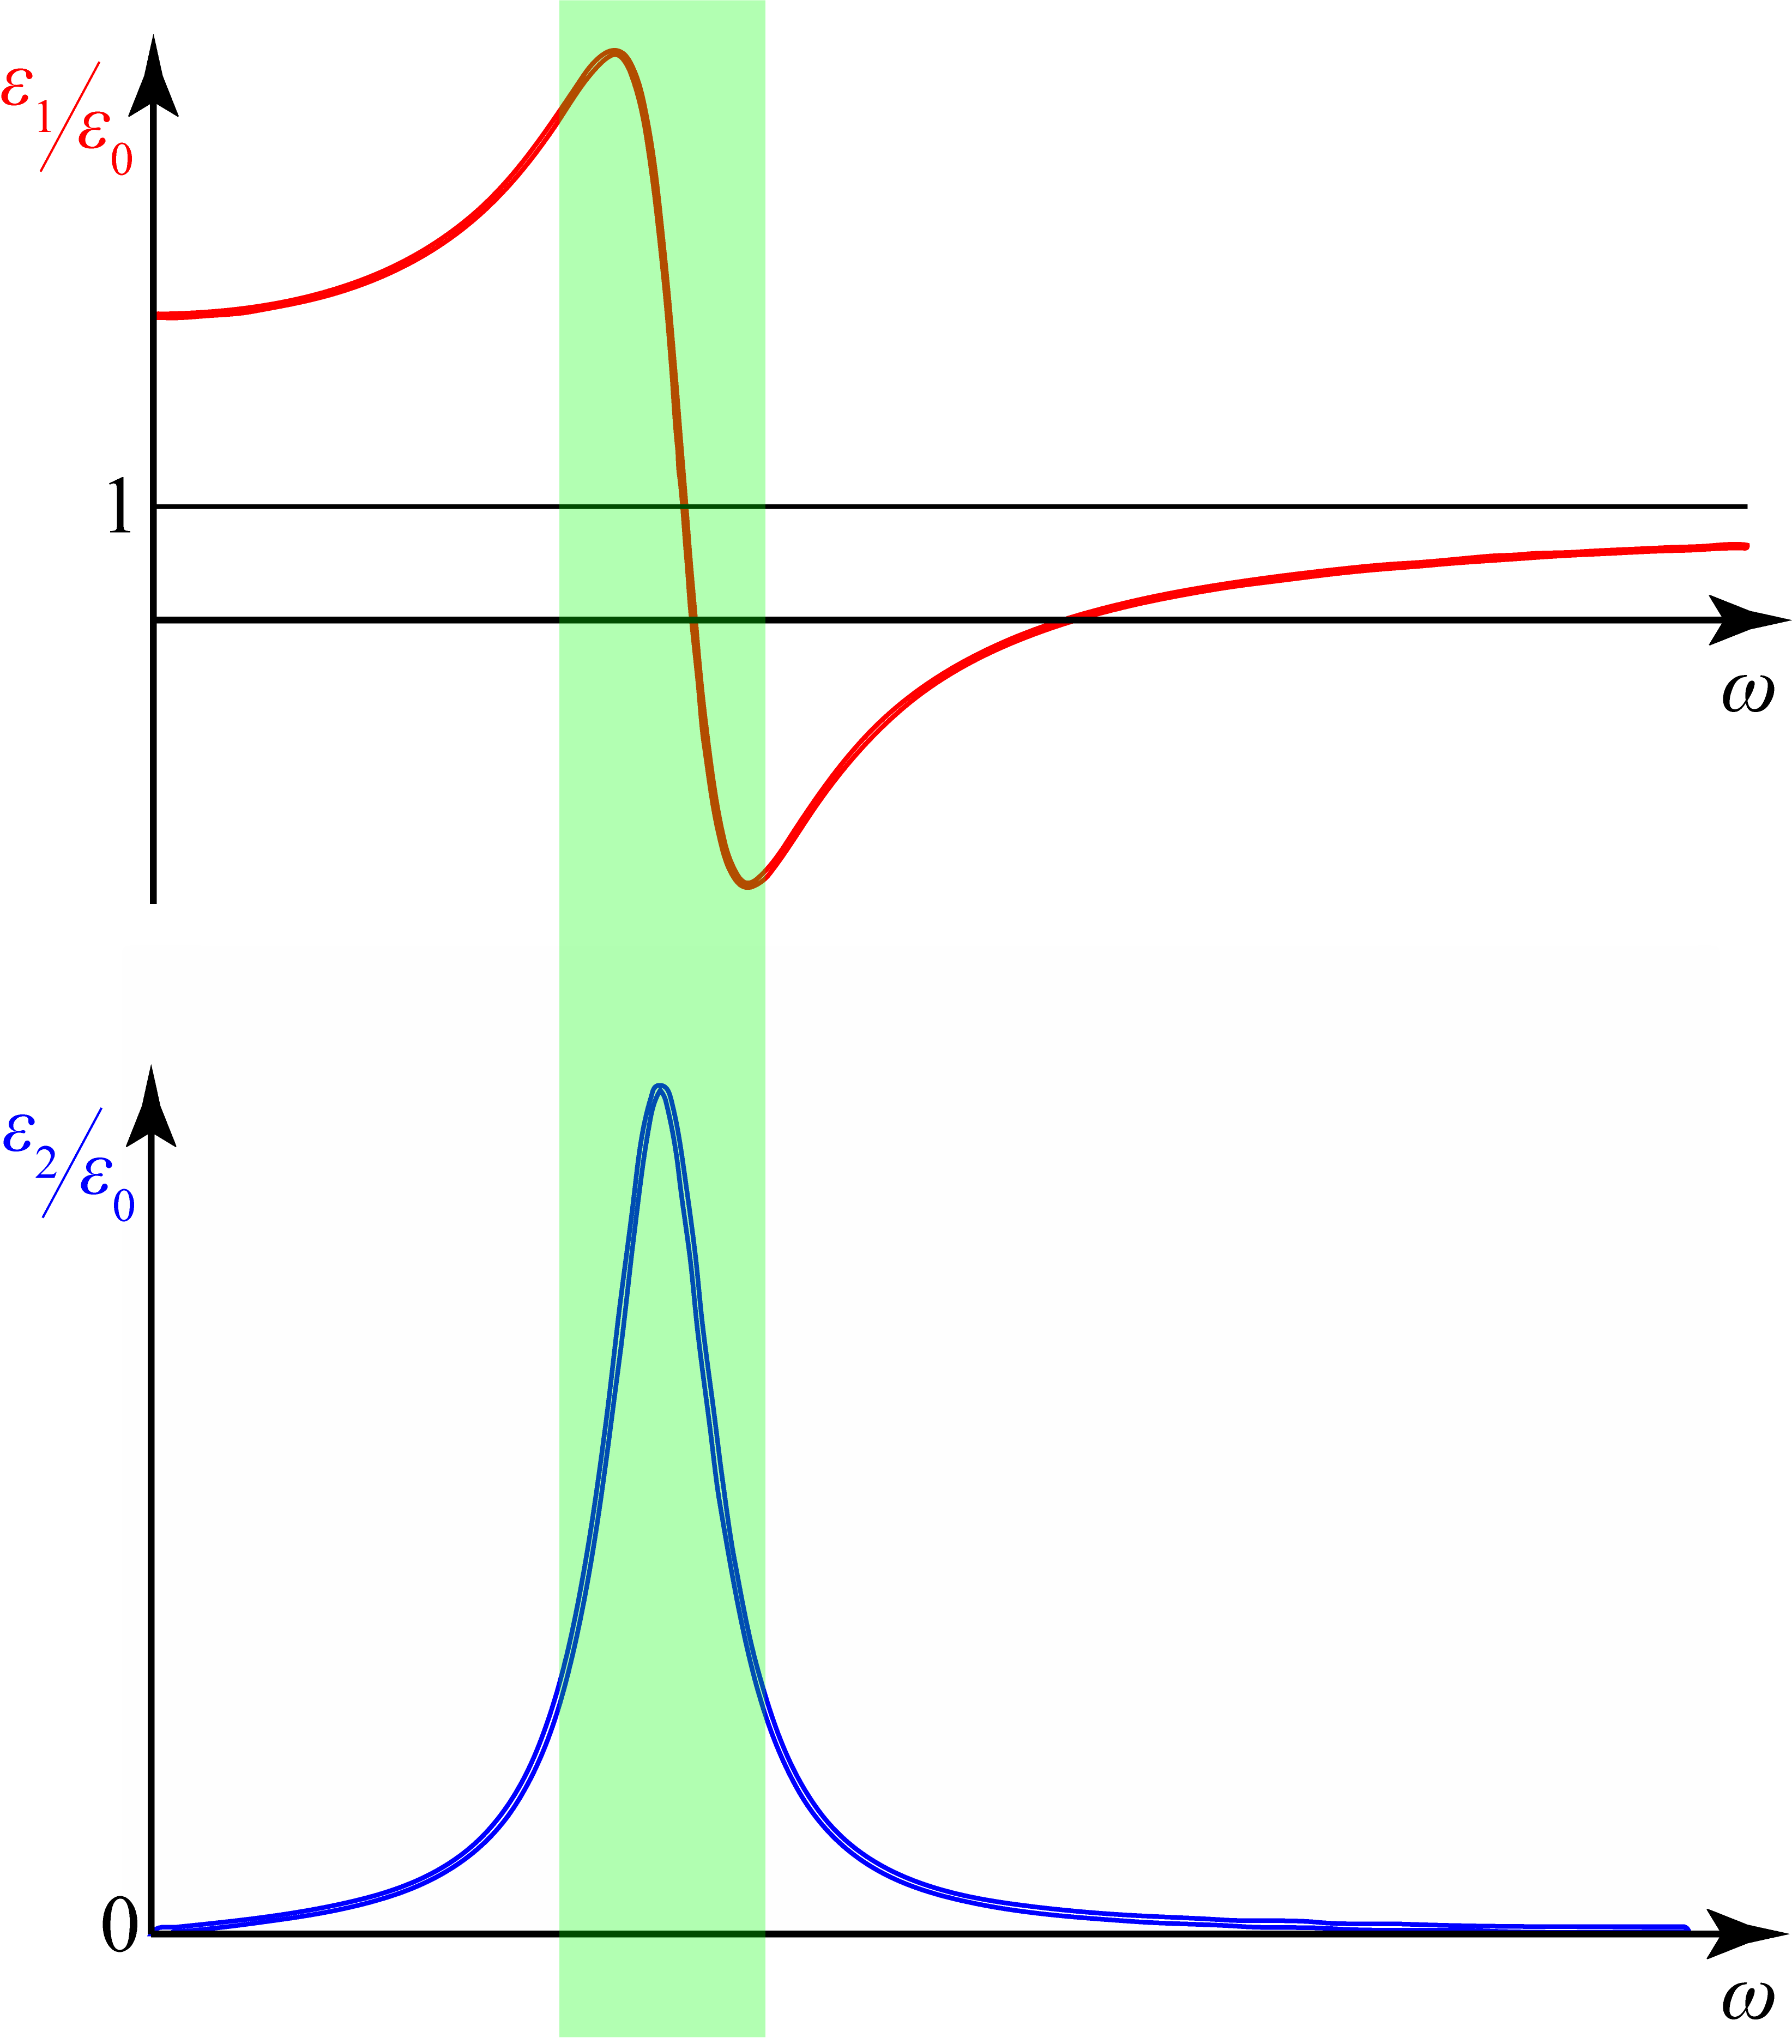
\includegraphics[width=6cm]{image/18-1-1.png}
\caption{复电容率与频率的关系}
\end{wrapfigure}
通常,\,把$nZe^2/\varepsilon_0 m$称作\emph{等离子体频率}(plasma frequency)的平方$\omega_p^2$.\,那么上式也作:
\[\varepsilon'=\varepsilon_0+\frac{\omega_p^2}{\omega_0^2-\omega^2-\ui\gamma\omega/m}\varepsilon_0\]

出现虚部其实就意味着损耗,\,在振动的过程中电场在持续不断地对振子输入能量而导致了电磁波的衰减.\,只不过这里的损耗并不是导电行为导致的.\,写出复电容率的实部和虚部$\varepsilon'=\varepsilon_1+\ui\varepsilon_2$:
\[\varepsilon_1=\varepsilon_0\cdot\left[1+\frac{\omega_p^2(\omega_0^2-\omega^2)}{(\omega_0^2-\omega^2)^2+(\gamma\omega/m)^2}\right]\]
\[\varepsilon_2=\varepsilon_0\cdot\frac{\gamma\omega_p^2\omega/m}{(\omega_0^2-\omega^2)^2+(\gamma\omega/m)^2}\]

两个函数看上去复杂,\,其实都属于近似的\emph{洛伦兹型函数}(lorentzian function).\,图像如右图所示.\,在绿色带状区域这个函数有着较大的转折.\,这发生在$\omega\approx \omega_0$处.\,若做近似,\,认为反应损耗的$\gamma$较小.\,则命$\omega^2-\omega_0^2=x$,\,$\gamma\omega_0/m=a$,\,那么上式在带状区域附近近似为标准的洛伦兹型:
\[\varepsilon_1/\varepsilon_0=1-\omega_p^2\cdot \frac{x}{x^2+a^2}\]
\[\varepsilon_2/\varepsilon_0=\omega_p^2\cdot\frac{a}{x^2+a^2}\]

电容率的实部在带状区域由区域外的缓慢增加转为剧烈减少,\,而恰好在这样一个区域,\,电容率的虚部突然变得很大.\,我们习惯上用虚部这种洛伦兹函数增加到最大值的一半的两个点之间的间距作为特征的\emph{半高峰宽}(full width at half maximum,\,FWHM).\,对于洛伦兹型,\,其值恰为$x=\pm a$之间的间距$2a$,\,但是注意到要转化为$\omega$对应的间距,\,它恰好为:
\[\Gamma=\frac{\gamma}{m}\]

我们可以从这个模型中清楚地看到两个物理现象:\,\emph{色散}(dispersion)与\emph{吸收}(absorption).\,前者就是说折射率依赖于波长,\,这和复电容率的实部依赖于频率只是说法不同本质一样.\,而复电容率的虚部,\,根据之前的讨论,\,也就代表吸收.\,我们发现在入射光的频率近似为谐振子的固有频率$\omega_0$时,\,对应经典力学中发生共振的区域附近,\,色散和吸收都变得很显著.\,我们知道,\,经典电子论给出的解释仅仅是一个唯象模型,\,所以相关的参数都要根据实验结果来确定.\,$\omega_0$可以根据发生强烈吸收与色散的波长来确定,\,而$\gamma/m$则根据吸收峰的半高峰宽$\Gamma$来确定,\,最后等离子体频率$\omega_p$则比较有趣,\,我们恰好可以根据零频率处的折射率$n_0$来确定它:
\[n_0^2=\varepsilon_1(0)/\varepsilon_0=1+\omega_p^2/\Gamma^2\]


那么实际情况是否这么简单呢?\,至少通过对右图的常温下水的色散的测量中我们发现,\,除了在可见光波段水几乎是透明的而具有大约$1.33$的折射率,\,在近红外(0.8-2.5${\rm \upmu m}$)与中红外(2.5-15${\rm \upmu m}$)波段的短波区定性上符合以上模型推导出来的结果.\,但是中红外到远红外(15-1000${\rm \upmu m}$)则明显偏离以上结果.
\begin{figure}[H]
\centering
\begin{minipage}{0.53\textwidth}
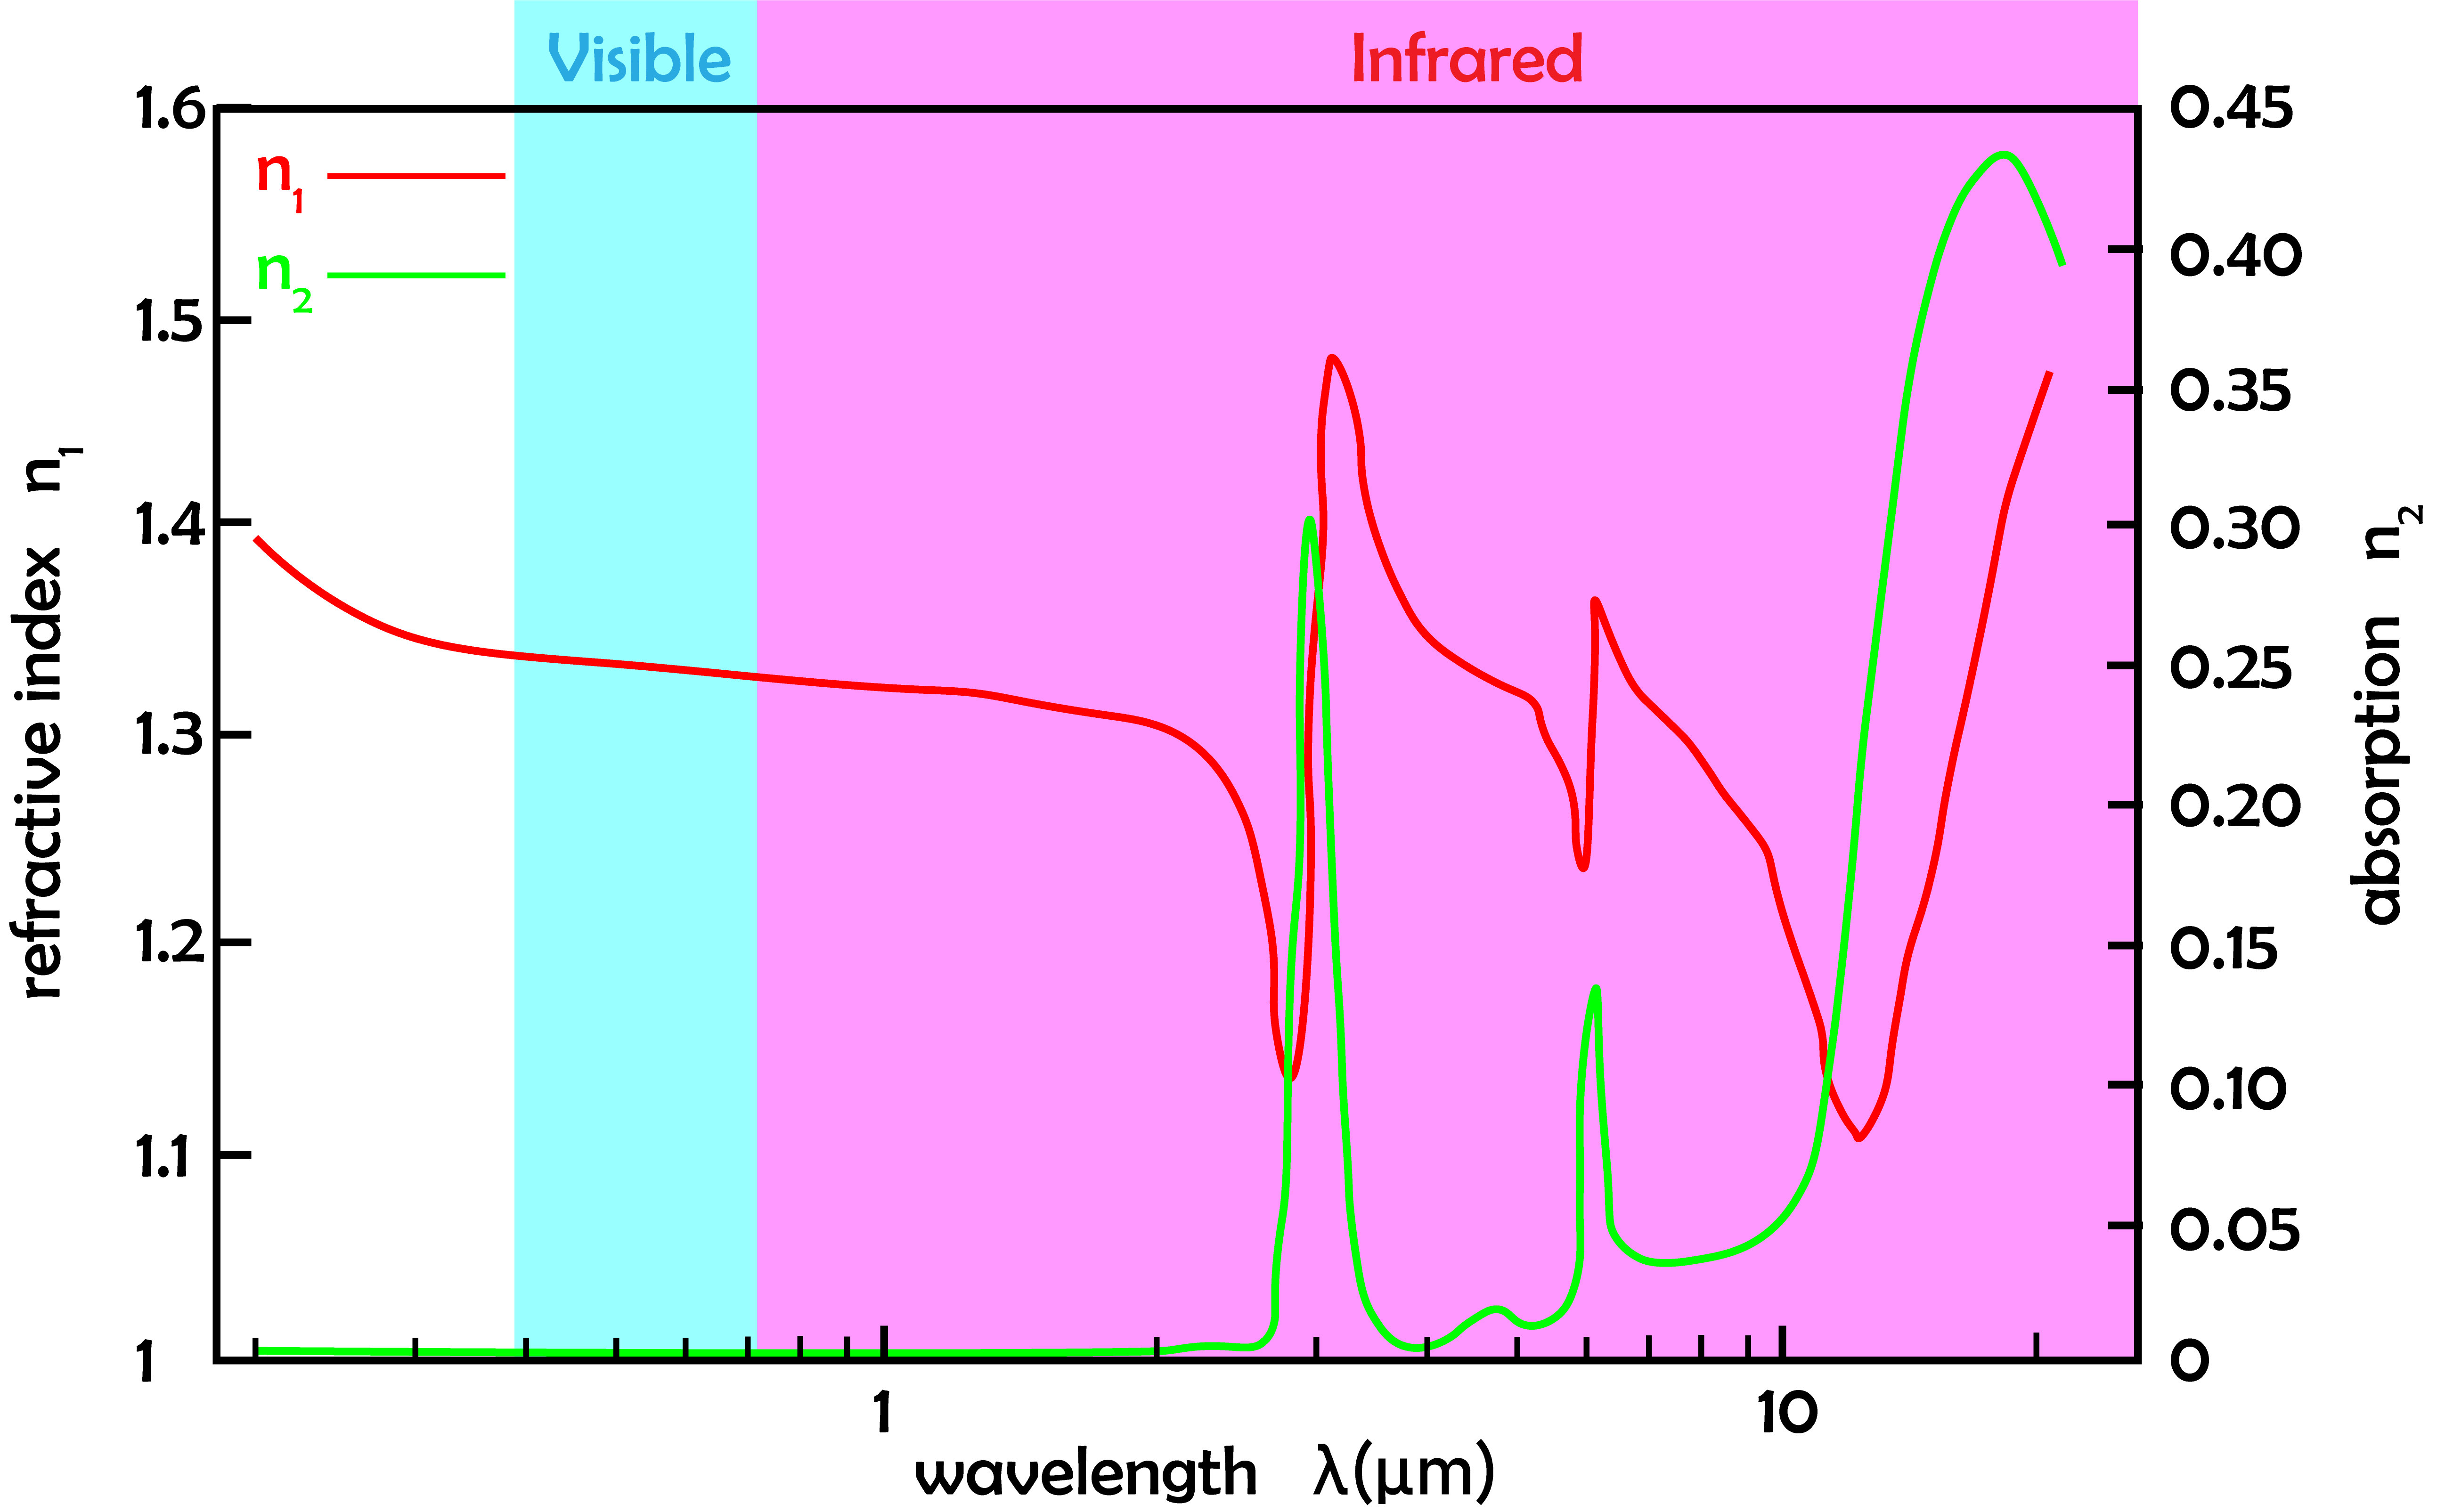
\includegraphics[width=\textwidth]{image/18-1-3.png}
\caption{水的可见-红外色散曲线}
\end{minipage}
\qquad
\begin{minipage}{0.38\textwidth}
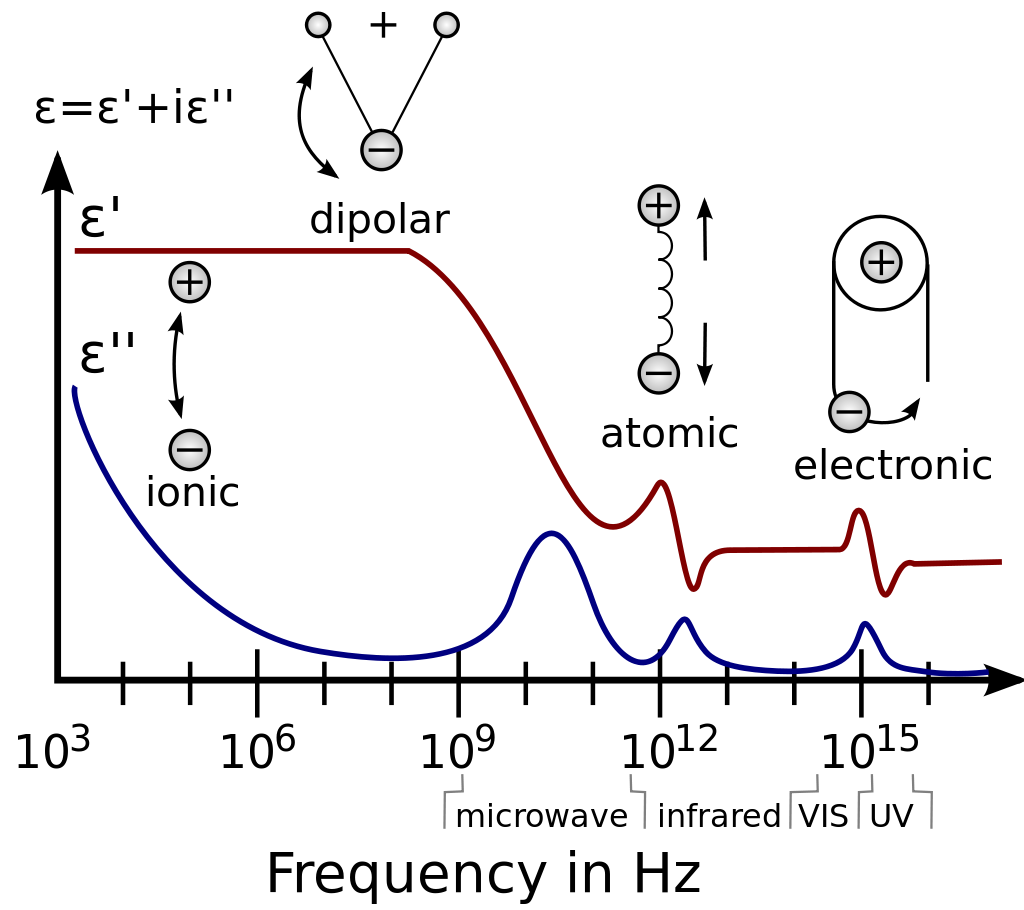
\includegraphics[width=\textwidth]{image/18-1-4.png}
\caption{光与原子作用类型}
\end{minipage}
\end{figure}

事实上,\,在不同的波段,\,适用于不同的光与物质相互作用的基本模型.\,微波波段光波长足够长使得晶体的正负离子做大范围的整体相对运动\footnote{十分类似于热运动的那种形式,\,区别在于这是外场诱导的有规律的振动,\,而且正负电荷位移一定反相,\,对应热振动的特定光学支.},\,就是晶格振动.\,红外则开始使得分子振动,\,包括转动和振动等不同形式.\,再往下的可见波段才是电子共振,\,也包括原子间的能带共振和原子内的能级共振.\,最后在紫外波段,\,电子甚至能直接被电离,\,这就造成了光与物质相互作用问题的复杂性.

但无论哪种相互作用的机制,\,我们上述推导得到的描述有着特定共振频率的色散与吸收的最终公式是十分普适的.\,它只有三个待定的参数:\,共振频率$\omega_0$,\,半高峰宽$\Gamma$和反应共振强度的等离子体频率$\omega_p$.\,我们接下来要做的,\,是把不同振子,\,不同吸收效应带来的结果进行求和:
\[\varepsilon_1/\varepsilon_0=1+\omega_p^2\cdot\sum_i\frac{c_i(\omega_i^2-\omega^2)}{(\omega_i^2-\omega^2)^2+\Gamma_i^2\omega^2}\]
\[\varepsilon_2/\varepsilon_0=\omega_p^2\cdot\sum_i\frac{c_i\Gamma_i\omega}{(\omega_i^2-\omega^2)^2+\Gamma_i^2\omega^2}\]

其中$\omega_p$仍然统计各个吸收峰的总强度,\,而$c_i$系数的和必须为1则统计各个吸收峰的相对强度.\,我们最后计算远离吸收带处的折射率值.\,忽略各个$\Gamma_i$后得到:
\[n^2=1+\omega_p^2\cdot\sum_i\frac{c_i}{\omega_i^2-\omega^2}\]

于是便得到著名的色散关系:
\[n^2=1+\sum_i a_i\cdot\frac{\lambda^2}{\lambda^2-\lambda_i^2}\quad,\quad a_i=\frac{c_i\omega_p^2\lambda_i^2}{4\pi^2}\]

上式依然可以做近似,\,把共振的各个波长$\lambda_i$从小到大按$i$来排列.\,不妨设$\lambda_i\ll\lambda_{i+1}$,\,而$\lambda$恰好夹在两者之间,\,那么:
\[n^2=\]


\section{色散,\,散射与吸收}

\section{群速与展宽}

\section{光量子}


%!TEX root = ../physical-olympics-2.tex
\chapter{量子论}

\begin{comment}

我们用选自\emph{费曼}(R. Feynman)先生的物理学讲义的开篇金句来作为本章与下一章近代物理内容的开头:
\begin{quote}
Each piece, or part, of the whole of nature is always merely an approximation to the complete truth. Therefore, things must be learned only to be unlearned again or, more likely, to be corrected. The test of all knowledge is \emph{experiment}. Experiment is the sole judge of scientific ``truth''.
\end{quote}

的确,\,量子理论以其不直观而被近代早期物理学家们所疑惑,\,这其中不乏一些赫赫有名的大师.\,直到现在也有很多基础的问题是没有被深刻地理解的:\,电子的本性与内部结构,\,基本粒子的类别与参数,\,对量子非定域性与测量的理解...\,所以在关于可能会造成问题的领域的学习时,\,需要先明白实验上的事实,\,从中理解理论建立的必要性.

\end{comment}


\section{黑体辐射}

\begin{comment}

对于\emph{热辐射}(thermal radiation)的讨论是何时进入物理研究的视野的呢?\,可以肯定的是人类认识到热辐射现象非常的早:\,光芒万丈的太阳,\,烧红的木炭与金属都是典型的热辐射的情形.\,但人们掌握足够的方法去测量它则也是要到19世纪后半期了.\,热辐射势必涉及到电磁场与电荷的相互作用.\,而且深入到原子尺度,\,实际上就是电磁波的发射与吸收.\,对于电磁波的发射,\,我们在电磁学中粗略讲过,\,只要有加速运动的电荷就会导致电磁辐射.\,之后小节我们将认识到微观电荷不能用``加速''来描述,\,其状态其实是量子态,\,处于激发态才会自发向基态去跃迁放出电磁辐射.\,而对于电磁波的吸收,\,则在光学中我们简要介绍过洛伦兹电子论中的处理方法.\,

\begin{wrapfigure}[9]{o}[0pt]{7cm}
\centering
\vspace{-15pt}
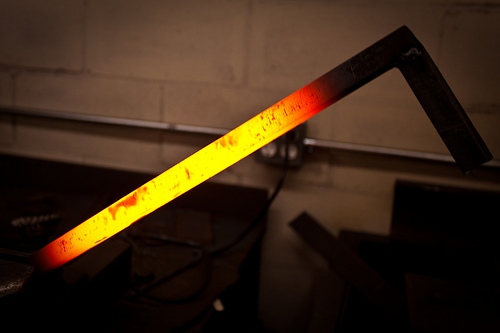
\includegraphics[width=7cm]{image/19-1-1.jpg}
\caption{热辐射}
\end{wrapfigure}
一个物体如果能够在任何温度下把照射到它上面的任何频率的光都全部吸收掉,\,那么这个物体就叫做\emph{黑体}(black body).\,虽然在现实生活中这样的物体并不存在,\,但石墨和碳黑往往被视作比较理想的黑体,\,尽管这样,\,黑体``看上去''也不总是``黑的''.\,著名生物学家查尔斯·达尔文的一个亲戚,\,陶瓷师,\,托马斯·玮致活在1792年注意到所有物体,\,不论化学构成,\,形状,\,尺寸,\,几乎都在相同的温度下烧红.\,黑体也不例外.\,作为这个实验现象研究的推广,\,1859年\emph{基尔霍夫}(G. Kirchhoff)利用热力学理论证明了著名的\emph{基尔霍夫定律}:\,即对于某角频率的光波,\,某温度下任意物体的辐射本领正比于吸收率:
\[e(\omega)=J(\omega,\,T)A(\omega)\]

其中,\,$e$为单位面积单位时间单位角频率间隔辐射的能量,\,而$A$为对该频率光的吸收率.\,$0<A<1$.\,除了吸收以外就是反射.\,物体较薄时还存在透射.\,不同物体在相同的$T,\,\omega$下可以有不同的$A,\,e$,\,但是其比值$J$却是一个\emph{普适}(universal)的函数.\,即与物体本身没有关系.\,而黑体的定义为$A(\omega)$恒等于$1$.\,也就是说明了黑体的辐射本领:
\[e(\omega)=J(\omega,\,T)\]

之后人们的任务就非常清晰了:\,测出不同$T$下的函数$J(\omega,\,T)$.\,而这个过程大致可以分为三个阶段:

1.\,挖掘出$J(\omega,\,T)$的整体特征.

2.\,实验测量$J(\omega,\,T)$的曲线与提出可能的理论模型.

3.\,最终确定$J(\omega,\,T)$的函数形式与理论解释.

\[J(\omega,\,T)=\frac{1}{4}u(\omega,\,T)c\]

\[u(\omega,\,T)=\frac{C_1\omega^3}{e^{C_2\omega/kT}-1}\]

\begin{wrapfigure}[9]{o}[0pt]{7cm}
\centering
\vspace{-15pt}
\includegraphics[width=7cm]{image/19-1-2.jpg}
\caption{真正的研究者}
\end{wrapfigure}
怎么去解释这个式子呢?\,从接触到黑体辐射谱的曲线开始,\,普朗克用了足足六年的时间才得到一个合理的解释.\,那是在1901年,\,功夫不负有心人,\,这位``真正的研究者''十分谨慎地发表了关于能量量子化的著名论文,\,科学研究史首次叩响了量子理论的大门.

普朗克的工作大致可以如此解释.\,我们
\end{comment}

\begin{itemize}
\item 黑体辐射的性质:
\begin{itemize}
\item 总辐射强度:
\[J=\sigma T^4=\frac{1}{4}uc\]
\[\sigma=5.67\times 10^-8{\rm W/(m^2\cdot K^4)}=\frac{2\pi^5 k^4}{15h^3c^2}\]

\item 辐射频域谱:\,普朗克公式:
\[J(\omega)=\frac{\hbar\omega^3}{4\pi^3c^2}\frac{1}{e^{\frac{\hbar\omega}{kT}}-1}\]

\item 辐射空间谱:\,郎伯定律:
\[\frac{\ud J}{\ud\Omega}=\frac{J}{\pi}\cos\theta\]
\end{itemize}

\item 非黑体满足基尔霍夫定律:\,某角频率$\omega$下发射率$e(\omega)$与吸收率$a(\omega)$必然相等.\,发射率是
\[\frac{\ud E}{\ud S\ud t}=\int E(\omega)\ud \omega\]
\[e(\omega)=E(\omega)/J(\omega)\]

故基尔霍夫定律发现:
\[e(\omega)=a(\omega)\]
\end{itemize}

\section{光粒子性}

\begin{itemize}
\item 光子概念:
\[E=\hbar\omega \quad ,\quad \bs{p}=\hbar \bs{k}\]

\item 用于解释普朗克公式:\,玻色-爱因斯坦统计.

\item 用于解释光电效应:
\[E_k=h\nu-W\geq eU\quad \rightarrow I\]
\end{itemize}

\section{玻尔原子}

\begin{itemize}
\item \emph{精细结构常数}(fine structure constant):
\[\alpha =\frac{e^2}{4\pi \varepsilon_0 \hbar c}\approx \frac{1}{137}\]

\item 半经典假设:\,忽略电子的波动性,\,认为仍然有轨道运动,\,且为圆周运动,\,符合牛顿力学:
\[m\frac{v_n^2}{r_n}=\frac{e^2
}{4\pi \varepsilon_0 r_n^2}\]

\item 量子化假设:\,角动量是量子化的,\,或者作用量量子化:
\[mv_n\cdot 2\pi r_n=nh\]

\item 定态跃迁假设:\,基态$n=1$是能量最低的稳定态,\,其他态与基态彼此之间都有可能发生转变,\,转变是瞬间发生的,\,伴随着一个光子的吸收或发射,\,且需要能量守恒:
\[E_n=\frac{1}{2}mv_n^2-\frac{e^2}{4\pi\varepsilon_0 r_n}\]
\[h\nu=E_n-E_m\]

\item 玻尔理论的解:
\[r_n=n^2 a_0\]
\[v_n=\frac{\alpha c}{n}\]
\[E_n=-\frac{E_0}{n^2}=-\frac{\alpha^2 mc^2}{2n^2}\]

其中$E_0$为第一电离能,\,氢原子为$13.6{\rm eV}$.\,而$a_0$为玻尔半径,\,它与另外两个特征长度:\,电子康普顿波长:
\[\lambda_e=\frac{h}{mc}\]

经典电子半径:
\[r_e=\frac{e^2}{4\pi\varepsilon_0 mc^2}\]

符合;
\[\alpha=\frac{\lambda_e/2\pi}{a_0}=\frac{a_0}{r_e}\]

\end{itemize}

%\section{电子波动性}

\section{物质波与波函数}

\begin{itemize}
\item 匀速运动的粒子对应一个平面波;
\[\psi=Ae^{\ui(\omega t-\bs{k}\cdot \bs{r})}\]

且符合德布罗意关系:
\[E=\hbar\omega\]
\[\bs{p}=\hbar\bs{k}\]

\item 对这个波的诠释:\,模方表示粒子在某空间点被探测到的概率分布函数:
\[f(\bs{r})=|\psi|^2\]
\[\int f(\bs{r})\ud V=1\]

\item 测不准原理:\,平面波情况下粒子位置是不确定的,\,但是动量却唯一.\,任意一个波函数可以分解为不同概率的平面波的叠加,\,那么某方向上位置和动量的两个不确定度(标准差)满足:
\[\Delta x\Delta p\geq \frac{\hbar}{2}\]

\end{itemize}

%!TEX root = ../physical-olympics-2.tex
\chapter{物理学尺度}


\section{宇观}

\section{宏观}

\section{介观}

\section{微观原子}

\section{微观亚原子}

	


\end{document}

%%%%%%%%%%%%%%%%%%%%%%%%%%%%%%%%%%%%%%%%%%%%%%%%%%%%%%%%%%%%%%%%%%%%%%%%%%%%%%